\documentclass[11pt,a4paper]{article}
\usepackage[utf8]{inputenc}\usepackage[T1]{fontenc}\usepackage{lmodern}
\usepackage[margin=1.9cm]{geometry}\usepackage[spanish]{babel}
\usepackage{graphicx}\usepackage{booktabs}\usepackage{longtable}\usepackage{array}
\usepackage{xcolor}\usepackage{fancyhdr}\usepackage{hyperref}\usepackage{titlesec}
\usepackage{listings}\usepackage{enumitem}
\definecolor{azul}{HTML}{0F5D4A}\definecolor{gris}{HTML}{555555}\definecolor{codebg}{HTML}{F6F6F6}
\hypersetup{colorlinks=true,linkcolor=azul,urlcolor=azul}
\pagestyle{fancy}\fancyhf{}\renewcommand{\headrulewidth}{0pt}
\fancyfoot[C]{\footnotesize\textcolor{gris}{Manual del Desarrollador · Igualab · \thepage}}
\titleformat{\section}{\Large\bfseries\color{azul}}{\thesection}{0.6em}{}
\titleformat{\subsection}{\large\bfseries\color{azul}}{\thesubsection}{0.5em}{}
\titleformat{\subsubsection}{\normalsize\bfseries}{\thesubsubsection}{0.4em}{}
\lstset{language=Python,basicstyle=\ttfamily\scriptsize,backgroundcolor=\color{codebg},
frame=single,rulecolor=\color{gray},breaklines=true,captionpos=b,aboveskip=3pt,belowskip=5pt,
keywordstyle=\color{azul}\bfseries,commentstyle=\color{gris}\itshape,stringstyle=\color{orange}}
\begin{document}
\begin{center}\vspace*{1cm}
{\Huge\bfseries\textcolor{azul}{Manual del Desarrollador}}\\[6pt]
{\LARGE Igualab · Arquitectura, Procesos y Código}\\[12pt]
{\large Backend FastAPI · 8 procesos (M1--M8) · 586 funciones documentadas}\\[6pt]
{\normalsize Documento técnico · generado 2026-10-15}\vspace{1cm}
\end{center}
\tableofcontents\newpage
\part{Visión general}\label{part:vision}
\section{Introducción}
Este manual explica \textbf{cómo está construido Igualab} a nivel de desarrollador: arquitectura, granularización por carpetas, la lógica de cada proceso, y una \textbf{referencia completa del código} (cada función, para qué sirve y su código). El código es la fuente de verdad.
\section{Arquitectura general}
Monolito modular con arquitectura por capas. Dos bases PostgreSQL 16 (transaccional + vectorial con \texttt{pgvector}).
\begin{figure}[h]\centering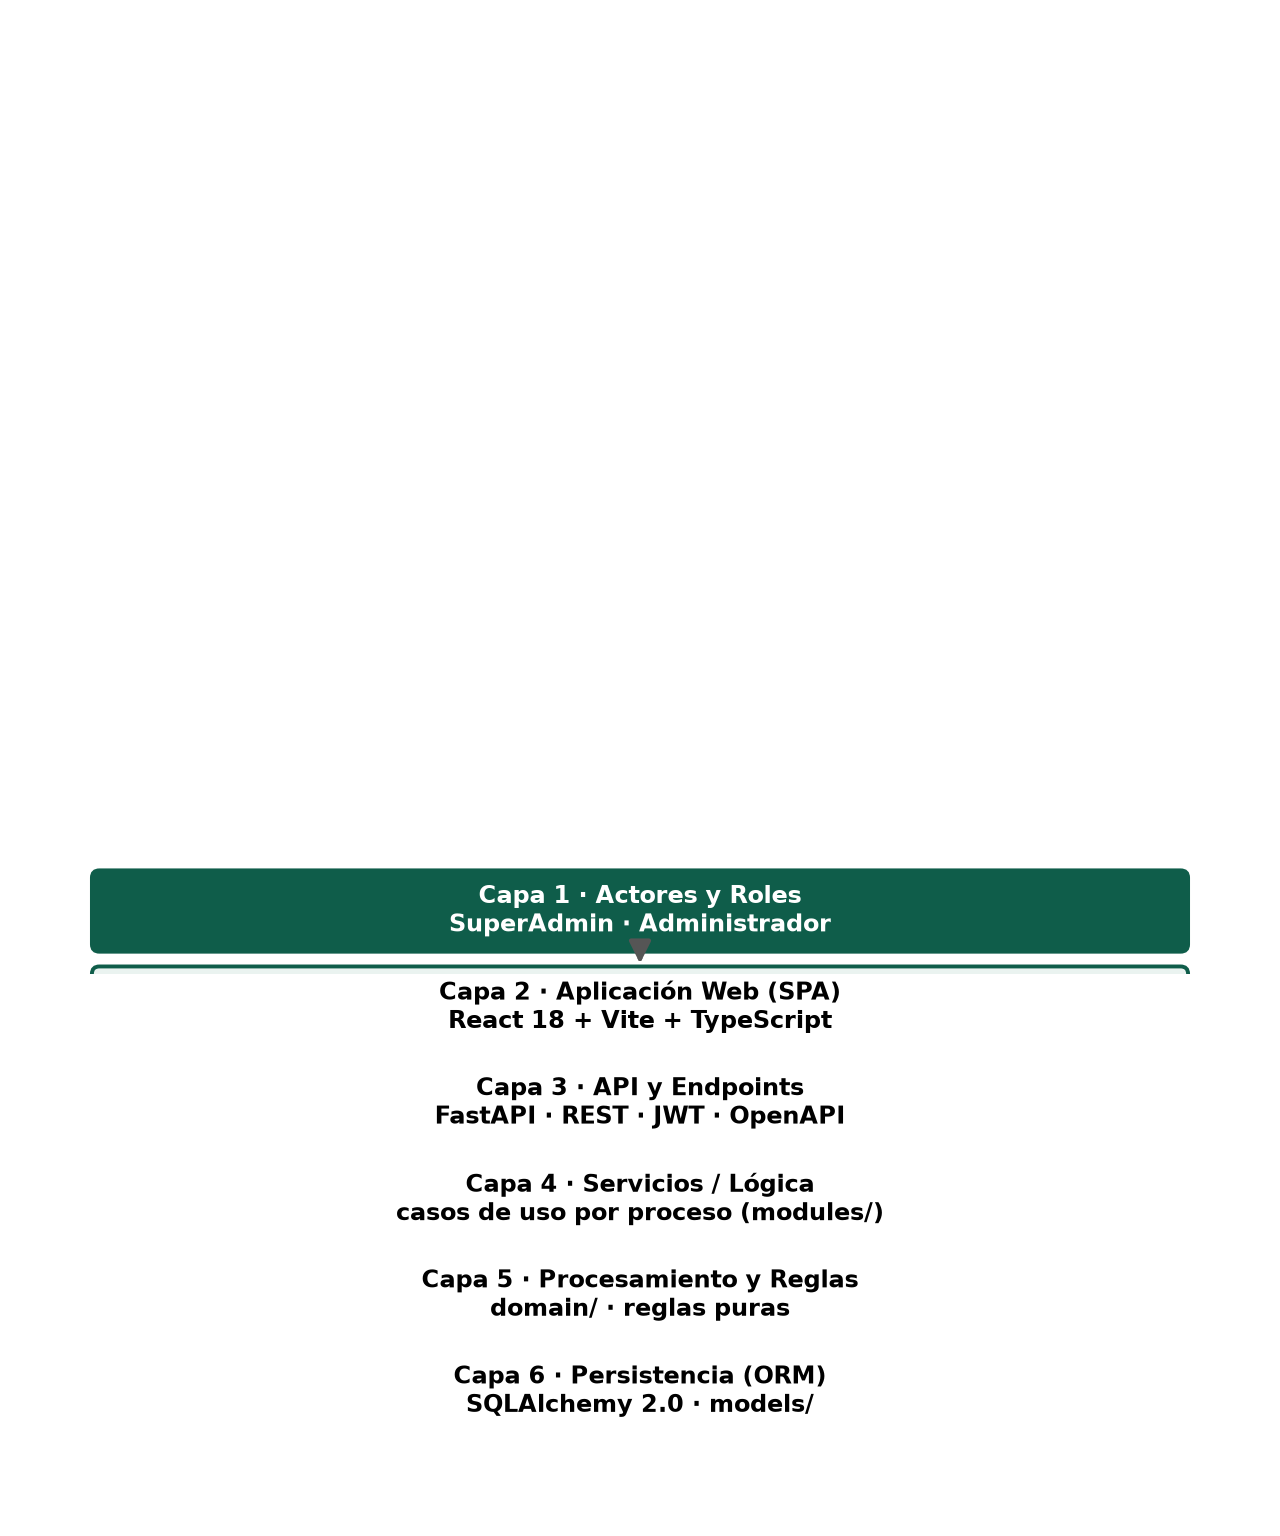
\includegraphics[width=0.8\textwidth]{img/capas.png}\caption{Arquitectura por capas.}\end{figure}
\section{Granularización}
3 niveles: \textbf{proceso} (módulo) $\rightarrow$ \textbf{responsabilidad} (\texttt{api}/\texttt{application}/\texttt{domain}/\texttt{infrastructure}) $\rightarrow$ \textbf{sub-proceso}. Regla: \emph{una carpeta = una razón para cambiar}.
\begin{figure}[h]\centering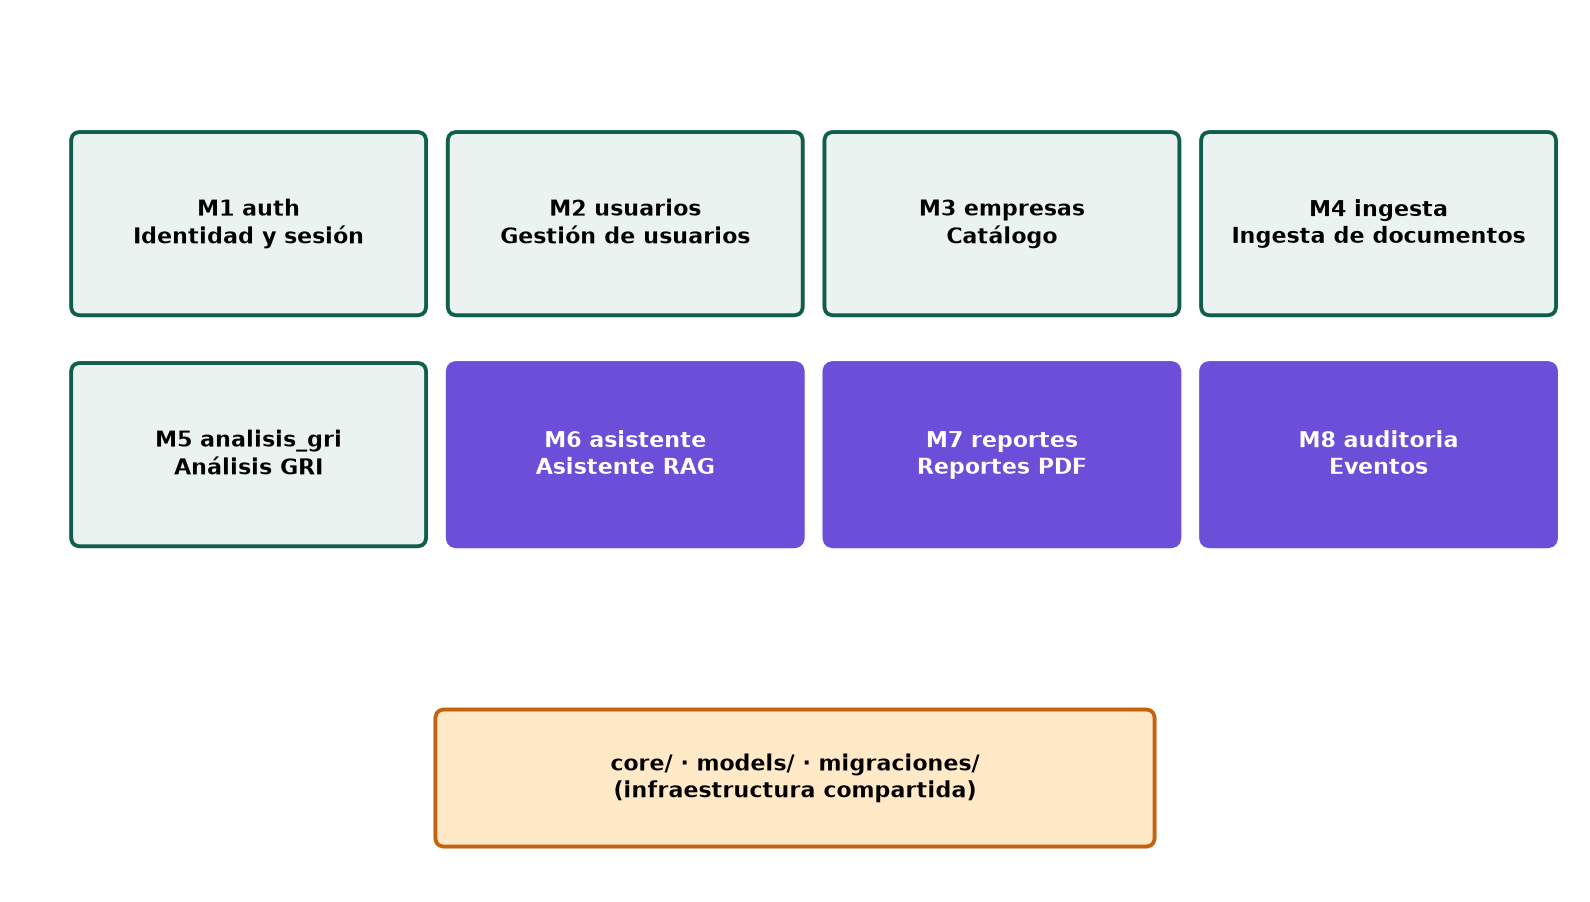
\includegraphics[width=0.92\textwidth]{img/procesos.png}\caption{Mapa de procesos (M1--M8).}\end{figure}
\section{Pipeline de Ingesta (M4)}
7 etapas: RESERVADO $\rightarrow$ ALMACENANDO\_ORIGINAL $\rightarrow$ INDEXANDO $\rightarrow$ ANALIZANDO $\rightarrow$ COMPLETANDO $\rightarrow$ PUBLICANDO $\rightarrow$ FINALIZADO. Ante fallo $\rightarrow$ compensación.
\begin{figure}[h]\centering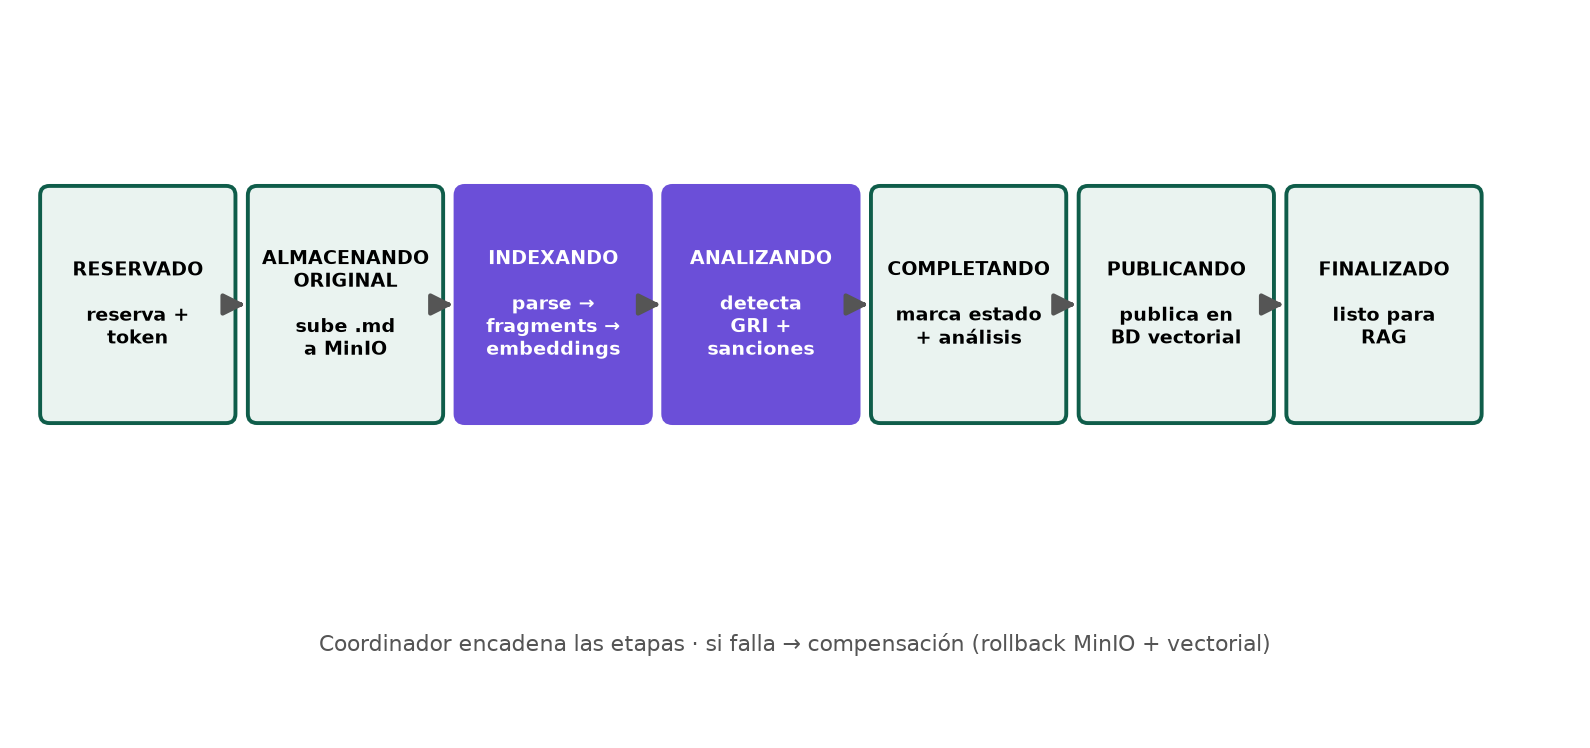
\includegraphics[width=0.95\textwidth]{img/pipeline_ingesta.png}\caption{Pipeline de ingesta.}\end{figure}
\section{Asistente IA (RAG) -- M6}
Pregunta $\rightarrow$ embedding de consulta $\rightarrow$ \texttt{buscar\_similares} (pgvector) $\rightarrow$ filtrar recuperables $\rightarrow$ prompt con contexto $\rightarrow$ LLM $\rightarrow$ citas verificadas.
\begin{figure}[h]\centering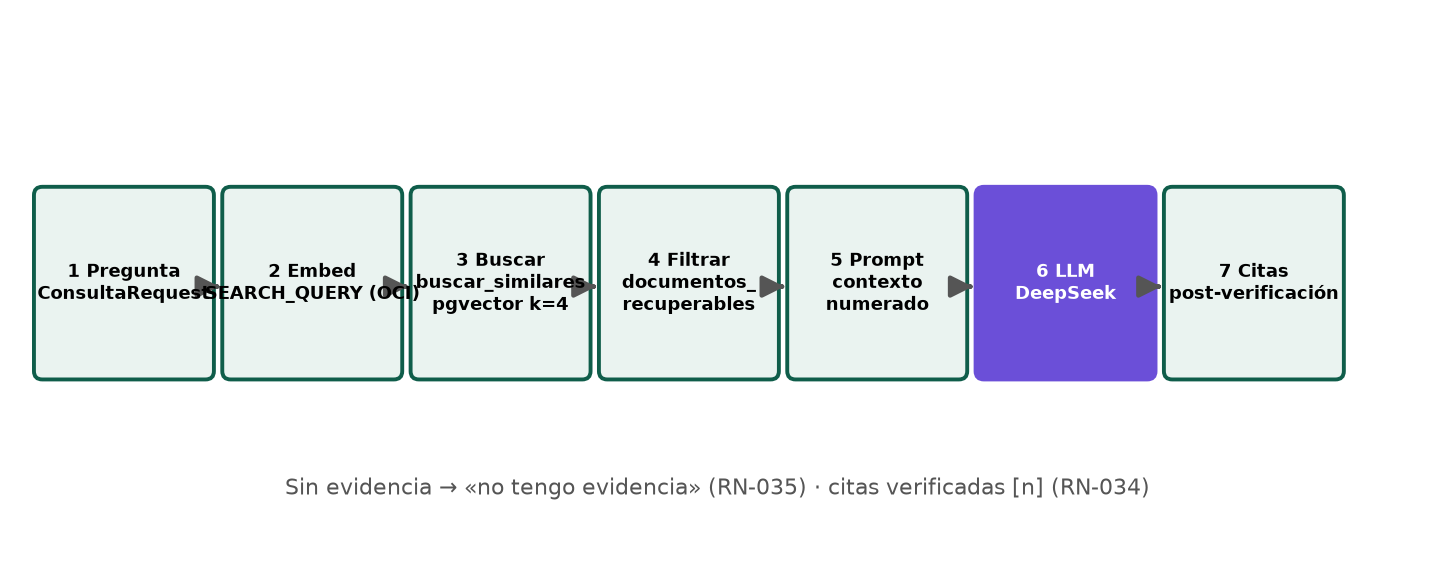
\includegraphics[width=0.9\textwidth]{img/rag.png}\caption{Flujo RAG.}\end{figure}
\section{Reportes de Prospección (M7)}
Plantilla LaTeX permanente + datos del análisis validado $\rightarrow$ tectonic $\rightarrow$ PDF. Render determinista (RN-040).
\begin{figure}[h]\centering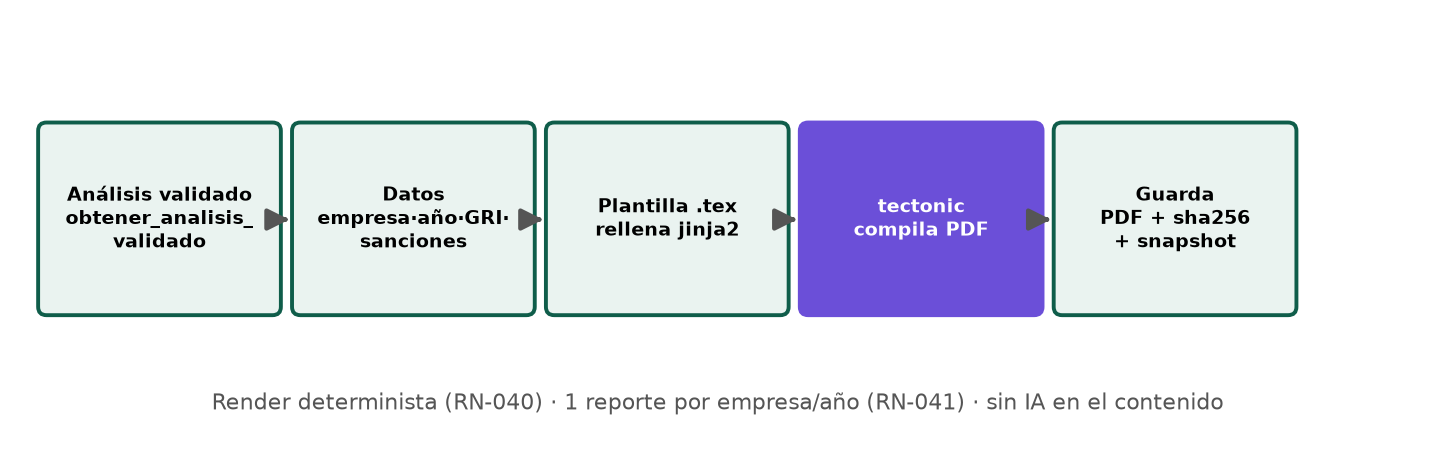
\includegraphics[width=0.9\textwidth]{img/reportes.png}\caption{Generación del reporte.}\end{figure}
\section{Variables de entorno}
Todo en el \texttt{.env}: \texttt{DATABASE\_URL}, \texttt{VECTOR\_DATABASE\_URL}, \texttt{JWT\_SECRET\_KEY}, \texttt{MINIO\_*}, \texttt{OCI\_*}, \texttt{DEEPSEEK\_*}, \texttt{APP\_ENV}.

\newpage\part{Referencia de código por módulo}\label{part:ref}
Cada función del backend con su firma, qué hace y su código fuente. Agrupado por módulo/submódulo.
\section{Parte II.1 · Infraestructura transversal -- \texttt{core/}}
\subsection{\texttt{core/config.py}}

\subsubsection*{\texttt{\_csv\_env}}
\textbf{Firma:} \texttt{\_csv\_env(name: str, default: str='') $\rightarrow$ list[str]}

\textbf{Qué hace:} (sin docstring)

\textbf{Código:}
\begin{lstlisting}
def _csv_env(name: str, default: str = "") -> list[str]:
    return [value.strip().rstrip("/") for value in os.getenv(name, default).split(",") if value.strip()]
\end{lstlisting}

\subsection{\texttt{core/database.py}}

\subsubsection*{\texttt{get\_db}}
\textbf{Firma:} \texttt{get\_db()}

\textbf{Qué hace:} (sin docstring)

\textbf{Código:}
\begin{lstlisting}
async def get_db():
    async with AsyncSessionLocal() as session:
        try:
            yield session
        except Exception:
            await session.rollback()
            raise
\end{lstlisting}

\subsection{\texttt{core/database\_vectorial.py}}
\textit{Conexión a la base de datos VECTORIAL (PostgreSQL + pgvector), independiente de la transaccional.}

\subsubsection*{\texttt{url\_vectorial}}
\textbf{Firma:} \texttt{url\_vectorial() $\rightarrow$ str}

\textbf{Qué hace:} URL configurada de la base vectorial; error controlado si falta o no es utilizable.

\textbf{Código:}
\begin{lstlisting}
def url_vectorial() -> str:
    """URL configurada de la base vectorial; error controlado si falta o no es utilizable."""
    url = settings.VECTOR_DATABASE_URL
    if not isinstance(url, str) or not url.strip():
        raise ExternalServiceError(
            "VECTOR_DATABASE_NOT_CONFIGURED",
            "La base de datos vectorial no está configurada: defina VECTOR_DATABASE_URL.",
        )
    url = url.strip()
    if not url.startswith(_PREFIJO):
        # No se repite el valor recibido: podría contener credenciales.
        raise ExternalServiceError(
            "VECTOR_DATABASE_URL_INVALID",
            "VECTOR_DATABASE_URL debe usar el controlador postgresql+asyncpg://.",
        )
    return url
\end{lstlisting}

\subsubsection*{\texttt{obtener\_motor\_vectorial}}
\textbf{Firma:} \texttt{obtener\_motor\_vectorial() $\rightarrow$ AsyncEngine}

\textbf{Qué hace:} Motor asíncrono de la base vectorial, creado la primera vez que se necesita.

\textbf{Código:}
\begin{lstlisting}
def obtener_motor_vectorial() -> AsyncEngine:
    """Motor asíncrono de la base vectorial, creado la primera vez que se necesita."""
    global _motor, _url_del_motor
    url = url_vectorial()
    if _motor is None or _url_del_motor != url:
        _motor = create_async_engine(url, echo=False)
        _url_del_motor = url
    return _motor
\end{lstlisting}

\subsubsection*{\texttt{fabrica\_sesiones\_vectoriales}}
\textbf{Firma:} \texttt{fabrica\_sesiones\_vectoriales() $\rightarrow$ async\_sessionmaker[AsyncSession]}

\textbf{Qué hace:} (sin docstring)

\textbf{Código:}
\begin{lstlisting}
def fabrica_sesiones_vectoriales() -> async_sessionmaker[AsyncSession]:
    return async_sessionmaker(obtener_motor_vectorial(), expire_on_commit=False)
\end{lstlisting}

\subsubsection*{\texttt{get\_vector\_db}}
\textbf{Firma:} \texttt{get\_vector\_db() $\rightarrow$ AsyncIterator[AsyncSession]}

\textbf{Qué hace:} Dependencia de FastAPI: una sesión vectorial por solicitud (nunca compartida entre tareas).

\textbf{Código:}
\begin{lstlisting}
async def get_vector_db() -> AsyncIterator[AsyncSession]:
    """Dependencia de FastAPI: una sesión vectorial por solicitud (nunca compartida entre tareas)."""
    async with fabrica_sesiones_vectoriales()() as sesion:
        try:
            yield sesion
        except Exception:
            await sesion.rollback()
            raise
\end{lstlisting}

\subsubsection*{\texttt{cerrar\_motor\_vectorial}}
\textbf{Firma:} \texttt{cerrar\_motor\_vectorial() $\rightarrow$ None}

\textbf{Qué hace:} (sin docstring)

\textbf{Código:}
\begin{lstlisting}
async def cerrar_motor_vectorial() -> None:
    global _motor, _url_del_motor
    if _motor is not None:
        await _motor.dispose()
    _motor, _url_del_motor = None, None
\end{lstlisting}

\subsection{\texttt{core/dependencies.py}}

\subsubsection*{\texttt{get\_current\_user}}
\textbf{Firma:} \texttt{get\_current\_user(credenciales: OptionalBearerCredentials, db: DatabaseSession) $\rightarrow$ Usuario}

\textbf{Qué hace:} Valida, en este orden:
  1. Que el token traiga una firma válida (RNF-003)
  2. Que la sesión (jti) exista, no esté revocada, y no haya expirado
     por inactividad
  3. Que la cuenta siga habilitada y con el rol que dice tener
     nunca se confía en el rol que trae el JWT si la
     cuenta cambió de rol después de emitido (RF-050)
Si todo pasa, actualiza ultima\_actividad (sesión deslizante) y
devuelve el Usuario

\textbf{Código:}
\begin{lstlisting}
async def get_current_user(
    credenciales: OptionalBearerCredentials,
    db: DatabaseSession,
) -> Usuario:
    """
    Valida, en este orden:
      1. Que el token traiga una firma válida (RNF-003)
      2. Que la sesión (jti) exista, no esté revocada, y no haya expirado
         por inactividad
      3. Que la cuenta siga habilitada y con el rol que dice tener
         nunca se confía en el rol que trae el JWT si la
         cuenta cambió de rol después de emitido (RF-050)
    Si todo pasa, actualiza ultima_actividad (sesión deslizante) y
    devuelve el Usuario
    """
    credenciales_invalidas = AuthenticationError(
        "INVALID_SESSION",
        "No autenticado o sesión inválida.",
        headers={"WWW-Authenticate": "Bearer"},
    )

    if credenciales is None:
        raise credenciales_invalidas

    token = credenciales.credentials
    payload = decodificar_token(token)

    if payload is None:
        raise credenciales_invalidas

    try:
        sesion_id = uuid.UUID(payload["jti"])
        usuario_id = uuid.UUID(payload["sub"])
    except (KeyError, ValueError):
        raise credenciales_invalidas

    sesion = await db.get(Sesion, sesion_id)
    if sesion is None or sesion.revocada or sesion.usuario_id != usuario_id:
        raise credenciales_invalidas

    ahora = datetime.now(timezone.utc)
    if ahora - sesion.ultima_actividad > settings.SESSION_INACTIVITY_TIMEOUT:
        sesion.revocada = True
        await db.commit()
        raise AuthenticationError(
            "SESSION_EXPIRED",
            "Sesión expirada por inactividad.",
            headers={"WWW-Authenticate": "Bearer"},
        )

    usuario = await db.get(Usuario, usuario_id)
    if usuario is None or not usuario.habilitado:
        raise credenciales_invalidas

    # cada petición autenticada renueva la ventana de inactividad
    sesion.ultima_actividad = ahora
    await db.commit()
    return usuario
\end{lstlisting}

\subsubsection*{\texttt{requerir\_rol}}
\textbf{Firma:} \texttt{requerir\_rol(*roles\_permitidos: RolUsuario)}

\textbf{Qué hace:} (sin docstring)

\textbf{Código:}
\begin{lstlisting}
def requerir_rol(*roles_permitidos: RolUsuario):
    def _verificar(
        usuario: CurrentUser,
    ) -> Usuario:
        if usuario.rol not in roles_permitidos:
            raise AuthorizationError(
                "FORBIDDEN",
                "No tiene permisos para esta acción.",
            )
        return usuario
    return _verificar
\end{lstlisting}

\subsection{\texttt{core/email\_service.py}}
\textit{Envío de correo (recuperación de contraseña). El `ConnectionConfig` de fastapi-mail se construye}

\subsubsection*{\texttt{\_configurado}}
\textbf{Firma:} \texttt{\_configurado() $\rightarrow$ bool}

\textbf{Qué hace:} True si hay correo remitente configurado (MAIL\_USERNAME y MAIL\_FROM).

\textbf{Código:}
\begin{lstlisting}
def _configurado() -> bool:
    """True si hay correo remitente configurado (MAIL_USERNAME y MAIL_FROM)."""
    return bool(settings.MAIL_USERNAME and settings.MAIL_FROM)
\end{lstlisting}

\subsubsection*{\texttt{\_construir\_config}}
\textbf{Firma:} \texttt{\_construir\_config() $\rightarrow$ ConnectionConfig}

\textbf{Qué hace:} (sin docstring)

\textbf{Código:}
\begin{lstlisting}
def _construir_config() -> ConnectionConfig:
    return ConnectionConfig(
        MAIL_USERNAME=settings.MAIL_USERNAME,
        MAIL_PASSWORD=settings.MAIL_PASSWORD,
        MAIL_FROM=settings.MAIL_FROM,
        MAIL_FROM_NAME=settings.MAIL_FROM_NAME,
        MAIL_SERVER=settings.MAIL_SERVER,
        MAIL_PORT=settings.MAIL_PORT,
        MAIL_STARTTLS=settings.MAIL_STARTTLS,
        MAIL_SSL_TLS=settings.MAIL_SSL_TLS,
        USE_CREDENTIALS=True,
    )
\end{lstlisting}

\subsubsection*{\texttt{enviar\_correo\_recuperacion}}
\textbf{Firma:} \texttt{enviar\_correo\_recuperacion(destinatario: str, token\_plano: str) $\rightarrow$ None}

\textbf{Qué hace:} (sin docstring)

\textbf{Código:}
\begin{lstlisting}
async def enviar_correo_recuperacion(destinatario: str, token_plano: str) -> None:
    if not _configurado():
        raise ServiceUnavailableError(
            "MAIL_NOT_CONFIGURED",
            "El envío de correos no está disponible: falta configurar MAIL_USERNAME / MAIL_FROM.",
        )
    try:
        mailer = FastMail(_construir_config())
    except Exception as exc:  # valores presentes pero inválidos (p. ej. MAIL_FROM sin '@')
        raise ServiceUnavailableError(
            "MAIL_NOT_CONFIGURED",
            "El envío de correos no está disponible: la configuración de correo es inválida.",
        ) from exc

    enlace = f"{settings.FRONTEND_RESET_URL}?token={token_plano}"
    mensaje = MessageSchema(
        subject="Igualab · Recuperación de contraseña",
        recipients=[destinatario],
        body=f"""
            <p>Recibimos una solicitud para restablecer tu contraseña.</p>
            <p><a href="{enlace}">Haz clic aquí para crear una nueva contraseña</a></p>
            <p>Este enlace vence en {settings.PASSWORD_RESET_TOKEN_EXPIRE_MINUTES} minutos. Si no solicitaste esto, ignora este correo.</p>
        """,
        subtype=MessageType.html,
    )
    await mailer.send_message(mensaje)
\end{lstlisting}

\subsection{\texttt{core/exception\_handlers.py}}

\subsubsection*{\texttt{\_request\_id}}
\textbf{Firma:} \texttt{\_request\_id(request: Request) $\rightarrow$ str}

\textbf{Qué hace:} (sin docstring)

\textbf{Código:}
\begin{lstlisting}
def _request_id(request: Request) -> str:
    return getattr(request.state, "request_id", "unavailable")
\end{lstlisting}

\subsubsection*{\texttt{\_error\_response}}
\textbf{Firma:} \texttt{\_error\_response(request: Request, *, status\_code: int, code: str, message: str, details: Any | None=None, headers: dict[str, str] | None=None) $\rightarrow$ JSONResponse}

\textbf{Qué hace:} (sin docstring)

\textbf{Código:}
\begin{lstlisting}
def _error_response(
    request: Request,
    *,
    status_code: int,
    code: str,
    message: str,
    details: Any | None = None,
    headers: dict[str, str] | None = None,
) -> JSONResponse:
    return JSONResponse(
        status_code=status_code,
        headers=headers,
        content=jsonable_encoder(
            {
                "error": {
                    "code": code,
                    "message": message,
                    "details": details,
                    "request_id": _request_id(request),
                }
            }
        ),
    )
\end{lstlisting}

\subsubsection*{\texttt{status\_for\_exception}}
\textbf{Firma:} \texttt{status\_for\_exception(exc: AppException) $\rightarrow$ int}

\textbf{Qué hace:} Estado HTTP según la jerarquía: la clase más específica de la MRO que tenga mapeo. Buscar solo el
tipo exacto enviaba a 400 a toda subclase (p. ej. PublicacionVectorialPendiente). Una subclase de
ExternalServiceTimeoutError es 504 y no 502 porque su clase aparece antes en la MRO.

\textbf{Código:}
\begin{lstlisting}
def status_for_exception(exc: AppException) -> int:
    """Estado HTTP según la jerarquía: la clase más específica de la MRO que tenga mapeo. Buscar solo el
    tipo exacto enviaba a 400 a toda subclase (p. ej. PublicacionVectorialPendiente). Una subclase de
    ExternalServiceTimeoutError es 504 y no 502 porque su clase aparece antes en la MRO."""
    for clase in type(exc).__mro__:
        estado = _STATUS_BY_EXCEPTION.get(clase)
        if estado is not None:
            return estado
    return status.HTTP_400_BAD_REQUEST
\end{lstlisting}

\subsubsection*{\texttt{app\_exception\_handler}}
\textbf{Firma:} \texttt{app\_exception\_handler(request: Request, exc: AppException) $\rightarrow$ JSONResponse}

\textbf{Qué hace:} (sin docstring)

\textbf{Código:}
\begin{lstlisting}
def app_exception_handler(
    request: Request,
    exc: AppException,
) -> JSONResponse:
    status_code = status_for_exception(exc)

    logger.warning(
        "Solicitud rechazada: code=%s request_id=%s",
        exc.code,
        _request_id(request),
    )

    return _error_response(
        request,
        status_code=status_code,
        code=exc.code,
        message=exc.message,
        details=exc.details,
        headers=exc.headers,
    )
\end{lstlisting}

\subsubsection*{\texttt{validation\_exception\_handler}}
\textbf{Firma:} \texttt{validation\_exception\_handler(request: Request, exc: RequestValidationError) $\rightarrow$ JSONResponse}

\textbf{Qué hace:} (sin docstring)

\textbf{Código:}
\begin{lstlisting}
def validation_exception_handler(
    request: Request, exc: RequestValidationError
) -> JSONResponse:
    # No se devuelve `input`: podría contener una contraseña u otro dato sensible.
    details = [
        {
            "location": list(error["loc"]),
            "message": error["msg"],
            "type": error["type"],
        }
        for error in exc.errors()
    ]
    return _error_response(
        request,
        status_code=status.HTTP_422_UNPROCESSABLE_ENTITY,
        code="REQUEST_VALIDATION_ERROR",
        message="La solicitud contiene datos inválidos.",
        details=details,
    )
\end{lstlisting}

\subsubsection*{\texttt{http\_exception\_handler}}
\textbf{Firma:} \texttt{http\_exception\_handler(request: Request, exc: StarletteHTTPException) $\rightarrow$ JSONResponse}

\textbf{Qué hace:} (sin docstring)

\textbf{Código:}
\begin{lstlisting}
def http_exception_handler(
    request: Request, exc: StarletteHTTPException
) -> JSONResponse:
    details = exc.detail if isinstance(exc.detail, (dict, list)) else None
    message = (
        exc.detail
        if isinstance(exc.detail, str)
        else "La solicitud no pudo completarse."
    )
    return _error_response(
        request,
        status_code=exc.status_code,
        code=_HTTP_ERROR_CODES.get(exc.status_code, "HTTP_ERROR"),
        message=message,
        details=details,
        headers=exc.headers,
    )
\end{lstlisting}

\subsubsection*{\texttt{\_internal\_error\_response}}
\textbf{Firma:} \texttt{\_internal\_error\_response(request: Request, exc: Exception, etiqueta: str) $\rightarrow$ JSONResponse}

\textbf{Qué hace:} Respuesta 500 uniforme (sin filtrar la causa). `etiqueta` solo cambia el mensaje de log.

\textbf{Código:}
\begin{lstlisting}
def _internal_error_response(request: Request, exc: Exception, etiqueta: str) -> JSONResponse:
    """Respuesta 500 uniforme (sin filtrar la causa). `etiqueta` solo cambia el mensaje de log."""
    logger.exception("%s: request_id=%s", etiqueta, _request_id(request), exc_info=exc)
    return _error_response(
        request,
        status_code=status.HTTP_500_INTERNAL_SERVER_ERROR,
        code="INTERNAL_ERROR",
        message="Ocurrió un error interno.",
    )
\end{lstlisting}

\subsubsection*{\texttt{database\_exception\_handler}}
\textbf{Firma:} \texttt{database\_exception\_handler(request: Request, exc: SQLAlchemyError) $\rightarrow$ JSONResponse}

\textbf{Qué hace:} (sin docstring)

\textbf{Código:}
\begin{lstlisting}
def database_exception_handler(
    request: Request, exc: SQLAlchemyError
) -> JSONResponse:
    return _internal_error_response(request, exc, "Error de base de datos")
\end{lstlisting}

\subsubsection*{\texttt{unexpected\_exception\_handler}}
\textbf{Firma:} \texttt{unexpected\_exception\_handler(request: Request, exc: Exception) $\rightarrow$ JSONResponse}

\textbf{Qué hace:} (sin docstring)

\textbf{Código:}
\begin{lstlisting}
def unexpected_exception_handler(request: Request, exc: Exception) -> JSONResponse:
    return _internal_error_response(request, exc, "Error inesperado")
\end{lstlisting}

\subsubsection*{\texttt{register\_exception\_handlers}}
\textbf{Firma:} \texttt{register\_exception\_handlers(app: FastAPI) $\rightarrow$ None}

\textbf{Qué hace:} (sin docstring)

\textbf{Código:}
\begin{lstlisting}
def register_exception_handlers(app: FastAPI) -> None:
    app.add_exception_handler(AppException, app_exception_handler)
    app.add_exception_handler(RequestValidationError, validation_exception_handler)
    app.add_exception_handler(StarletteHTTPException, http_exception_handler)
    app.add_exception_handler(SQLAlchemyError, database_exception_handler)
    app.add_exception_handler(Exception, unexpected_exception_handler)
\end{lstlisting}

\subsection{\texttt{core/exceptions.py}}

\subsubsection*{\texttt{es\_codigo\_valido}}
\textbf{Firma:} \texttt{es\_codigo\_valido(codigo: object) $\rightarrow$ bool}

\textbf{Qué hace:} True si `codigo` es un código de error estable y seguro (constante propia de la app).

\textbf{Código:}
\begin{lstlisting}
def es_codigo_valido(codigo: object) -> bool:
    """True si `codigo` es un código de error estable y seguro (constante propia de la app)."""
    return isinstance(codigo, str) and _CODIGO_REGEX.fullmatch(codigo) is not None
\end{lstlisting}

\subsubsection*{\texttt{codigo\_seguro}}
\textbf{Firma:} \texttt{codigo\_seguro(exc: BaseException, tipo: type[AppException]=None) $\rightarrow$ str}

\textbf{Qué hace:} Código estable y seguro del fallo: solo se reutiliza el `code` de una `AppException` del tipo
indicado (por defecto `AppException`); cualquier otra excepción (de terceros) es `UNEXPECTED\_ERROR`
y nunca se repite su mensaje.

\textbf{Código:}
\begin{lstlisting}
def codigo_seguro(exc: BaseException, tipo: type[AppException] = None) -> str:  # type: ignore[assignment]
    """Código estable y seguro del fallo: solo se reutiliza el `code` de una `AppException` del tipo
    indicado (por defecto `AppException`); cualquier otra excepción (de terceros) es `UNEXPECTED_ERROR`
    y nunca se repite su mensaje."""
    tipo = AppException if tipo is None else tipo
    codigo = getattr(exc, "code", None) if isinstance(exc, tipo) else None
    return codigo if es_codigo_valido(codigo) else "UNEXPECTED_ERROR"
\end{lstlisting}

\subsubsection*{\texttt{AppException.\_\_init\_\_}}
\textbf{Firma:} \texttt{AppException.\_\_init\_\_(self, code: str, message: str, details: Any | None=None, headers: dict[str, str] | None=None) $\rightarrow$ None}

\textbf{Qué hace:} (sin docstring)

\textbf{Código:}
\begin{lstlisting}
def __init__(
        self,
        code: str,
        message: str,
        details: Any | None = None,
        headers: dict[str, str] | None = None,
    ) -> None:
        super().__init__(message)
        self.code = code
        self.message = message
        self.details = details
        self.headers = headers
\end{lstlisting}

\subsection{\texttt{core/logging\_config.py}}

\subsubsection*{\texttt{configure\_logging}}
\textbf{Firma:} \texttt{configure\_logging() $\rightarrow$ None}

\textbf{Qué hace:} Configura logs locales sin interferir con los handlers de Uvicorn.

\textbf{Código:}
\begin{lstlisting}
def configure_logging() -> None:
    """Configura logs locales sin interferir con los handlers de Uvicorn."""
    root_logger = logging.getLogger()
    if not root_logger.handlers:
        logging.basicConfig(
            level=logging.INFO,
            format="%(asctime)s %(levelname)s %(name)s %(message)s",
        )
    logging.getLogger("igualab").setLevel(logging.INFO)
\end{lstlisting}

\subsubsection*{\texttt{paso\_de\_arranque}}
\textbf{Firma:} \texttt{paso\_de\_arranque(logger: logging.Logger, paso: str)}

\textbf{Qué hace:} Registra INFO al iniciar y al terminar un paso del arranque, con su duración. Si el paso falla o se interrumpe también lo
registra (solo la CLASE de la excepción: su mensaje puede contener hosts o credenciales) y vuelve a lanzarla. No cambia el
comportamiento del paso. Un `inicio` sin su `fin` en el log indica el paso en el que la aplicación sigue esperando.

\textbf{Código:}
\begin{lstlisting}
def paso_de_arranque(logger: logging.Logger, paso: str):
    """Registra INFO al iniciar y al terminar un paso del arranque, con su duración. Si el paso falla o se interrumpe también lo
    registra (solo la CLASE de la excepción: su mensaje puede contener hosts o credenciales) y vuelve a lanzarla. No cambia el
    comportamiento del paso. Un `inicio` sin su `fin` en el log indica el paso en el que la aplicación sigue esperando."""
    logger.info("Arranque | %s | inicio", paso)
    inicio = time.monotonic()
    try:
        yield
    except BaseException as exc:
        logger.error("Arranque | %s | falló o se interrumpió tras %.2f s (%s)", paso, time.monotonic() - inicio, type(exc).__name__)
        raise
    logger.info("Arranque | %s | fin en %.2f s", paso, time.monotonic() - inicio)
\end{lstlisting}

\subsection{\texttt{core/request\_id.py}}

\subsubsection*{\texttt{\_valid\_request\_id}}
\textbf{Firma:} \texttt{\_valid\_request\_id(value: str | None) $\rightarrow$ str}

\textbf{Qué hace:} (sin docstring)

\textbf{Código:}
\begin{lstlisting}
def _valid_request_id(value: str | None) -> str:
    if value:
        try:
            return str(uuid.UUID(value))
        except (ValueError, AttributeError):
            pass
    return str(uuid.uuid4())
\end{lstlisting}

\subsubsection*{\texttt{RequestIDMiddleware.\_\_init\_\_}}
\textbf{Firma:} \texttt{RequestIDMiddleware.\_\_init\_\_(self, app: ASGIApp) $\rightarrow$ None}

\textbf{Qué hace:} (sin docstring)

\textbf{Código:}
\begin{lstlisting}
def __init__(self, app: ASGIApp) -> None:
        self.app = app
\end{lstlisting}

\subsubsection*{\texttt{RequestIDMiddleware.\_\_call\_\_}}
\textbf{Firma:} \texttt{RequestIDMiddleware.\_\_call\_\_(self, scope: Scope, receive: Receive, send: Send) $\rightarrow$ None}

\textbf{Qué hace:} (sin docstring)

\textbf{Código:}
\begin{lstlisting}
async def __call__(self, scope: Scope, receive: Receive, send: Send) -> None:
        if scope["type"] != "http":
            await self.app(scope, receive, send)
            return

        headers = dict(scope.get("headers", []))
        raw_request_id = headers.get(b"x-request-id")
        supplied_request_id = (
            raw_request_id.decode("ascii", errors="ignore") if raw_request_id else None
        )
        request_id = _valid_request_id(supplied_request_id)
        scope.setdefault("state", {})["request_id"] = request_id

        async def send_with_request_id(message: Message) -> None:
            if message["type"] == "http.response.start":
                response_headers = list(message.get("headers", []))
                response_headers.append((b"x-request-id", request_id.encode("ascii")))
                message["headers"] = response_headers
            await send(message)

        await self.app(scope, receive, send_with_request_id)
\end{lstlisting}

\subsection{\texttt{core/security.py}}

\subsubsection*{\texttt{hash\_password}}
\textbf{Firma:} \texttt{hash\_password(password: str) $\rightarrow$ str}

\textbf{Qué hace:} (sin docstring)

\textbf{Código:}
\begin{lstlisting}
def hash_password(password: str) -> str:
    return _pwd_context.hash(password)
\end{lstlisting}

\subsubsection*{\texttt{verificar\_password}}
\textbf{Firma:} \texttt{verificar\_password(password\_plano: str, password\_hash: str) $\rightarrow$ bool}

\textbf{Qué hace:} (sin docstring)

\textbf{Código:}
\begin{lstlisting}
def verificar_password(password_plano: str, password_hash: str) -> bool:
    return _pwd_context.verify(password_plano, password_hash)
\end{lstlisting}

\subsubsection*{\texttt{validar\_politica\_password}}
\textbf{Firma:} \texttt{validar\_politica\_password(password: str, correo: str) $\rightarrow$ list[str]}

\textbf{Qué hace:} (sin docstring)

\textbf{Código:}
\begin{lstlisting}
def validar_politica_password(password: str, correo: str) -> list[str]:
    errores: list[str] = []
    if len(password) < 8:
        errores.append("La contraseña debe tener al menos 8 caracteres.")
    if not re.search(r"[A-Z]", password):
        errores.append("La contraseña debe incluir al menos una letra mayúscula.")
    if not re.search(r"[a-z]", password):
        errores.append("La contraseña debe incluir al menos una letra minúscula.")
    if not re.search(r"\d", password):
        errores.append("La contraseña debe incluir al menos un dígito.")
    if not re.search(r"[^\w\s]", password):
        errores.append("La contraseña debe incluir al menos un carácter especial.")
    if correo and password.lower() == correo.lower():
        errores.append("La contraseña no puede coincidir con el correo de la cuenta.")
    return errores
\end{lstlisting}

\subsubsection*{\texttt{crear\_access\_token}}
\textbf{Firma:} \texttt{crear\_access\_token(usuario\_id: uuid.UUID, rol: str, sesion\_id: uuid.UUID) $\rightarrow$ str}

\textbf{Qué hace:} (sin docstring)

\textbf{Código:}
\begin{lstlisting}
def crear_access_token(usuario_id: uuid.UUID, rol: str, sesion_id: uuid.UUID) -> str:

    ahora = datetime.now(timezone.utc)
    payload = {
        "sub": str(usuario_id),
        "rol": rol,
        "jti": str(sesion_id),
        "iat": ahora,
        "exp": ahora + timedelta(hours=8),
    }
    return jwt.encode(payload, settings.JWT_SECRET_KEY, algorithm=settings.JWT_ALGORITHM)
\end{lstlisting}

\subsubsection*{\texttt{decodificar\_token}}
\textbf{Firma:} \texttt{decodificar\_token(token: str) $\rightarrow$ dict | None}

\textbf{Qué hace:} (sin docstring)

\textbf{Código:}
\begin{lstlisting}
def decodificar_token(token: str) -> dict | None:
    try:
        return jwt.decode(token, settings.JWT_SECRET_KEY, algorithms=[settings.JWT_ALGORITHM])
    except JWTError:
        return None
\end{lstlisting}

\subsubsection*{\texttt{generar\_token\_recuperacion}}
\textbf{Firma:} \texttt{generar\_token\_recuperacion() $\rightarrow$ str}

\textbf{Qué hace:} (sin docstring)

\textbf{Código:}
\begin{lstlisting}
def generar_token_recuperacion() -> str:
    return secrets.token_urlsafe(32)
\end{lstlisting}

\subsubsection*{\texttt{hash\_token\_recuperacion}}
\textbf{Firma:} \texttt{hash\_token\_recuperacion(token: str) $\rightarrow$ str}

\textbf{Qué hace:} (sin docstring)

\textbf{Código:}
\begin{lstlisting}
def hash_token_recuperacion(token: str) -> str:
    return _pwd_context.hash(token)
\end{lstlisting}

\subsubsection*{\texttt{verificar\_token\_recuperacion}}
\textbf{Firma:} \texttt{verificar\_token\_recuperacion(token\_plano: str, token\_hash: str) $\rightarrow$ bool}

\textbf{Qué hace:} (sin docstring)

\textbf{Código:}
\begin{lstlisting}
def verificar_token_recuperacion(token_plano: str, token_hash: str) -> bool:
    return _pwd_context.verify(token_plano, token_hash)
\end{lstlisting}

\section{Parte II.2 · Modelos ORM -- \texttt{models/}}
\subsection{\texttt{models/analisis\_gri.py}}
\textit{Modelos del Módulo 5: análisis y validación de brechas GRI (CU005).}

\subsubsection*{\texttt{\_ahora\_utc}}
\textbf{Firma:} \texttt{\_ahora\_utc() $\rightarrow$ datetime}

\textbf{Qué hace:} (sin docstring)

\textbf{Código:}
\begin{lstlisting}
def _ahora_utc() -> datetime:
    return datetime.now(timezone.utc)
\end{lstlisting}

\subsection{\texttt{models/documento\_ingesta.py}}
\textit{Modelo transaccional de documentos de ingesta (Etapa 4A).}

\subsubsection*{\texttt{\_ahora\_utc}}
\textbf{Firma:} \texttt{\_ahora\_utc() $\rightarrow$ datetime}

\textbf{Qué hace:} (sin docstring)

\textbf{Código:}
\begin{lstlisting}
def _ahora_utc() -> datetime:
    return datetime.now(timezone.utc)
\end{lstlisting}

\subsubsection*{\texttt{\_vigencia\_inicial}}
\textbf{Firma:} \texttt{\_vigencia\_inicial() $\rightarrow$ datetime}

\textbf{Qué hace:} (sin docstring)

\textbf{Código:}
\begin{lstlisting}
def _vigencia_inicial() -> datetime:
    return _ahora_utc() + VIGENCIA_PREDETERMINADA
\end{lstlisting}

\subsubsection*{\texttt{\_enum}}
\textbf{Firma:} \texttt{\_enum(clase: type[enum.Enum], nombre: str) $\rightarrow$ Enum}

\textbf{Qué hace:} (sin docstring)

\textbf{Código:}
\begin{lstlisting}
def _enum(clase: type[enum.Enum], nombre: str) -> Enum:
    return Enum(clase, name=nombre, validate_strings=True)
\end{lstlisting}

\subsubsection*{\texttt{Documento.publicacion\_vectorial\_pendiente}}
\textbf{Firma:} \texttt{Documento.publicacion\_vectorial\_pendiente(self) $\rightarrow$ bool}

\textbf{Qué hace:} COMPLETADO en la base transaccional pero con los fragmentos aún sin publicar: situación
recuperable (se repite `publicar\_fragmentos`, idempotente, sin nuevos embeddings ni análisis).

\textbf{Código:}
\begin{lstlisting}
def publicacion_vectorial_pendiente(self) -> bool:
        """COMPLETADO en la base transaccional pero con los fragmentos aún sin publicar: situación
        recuperable (se repite `publicar_fragmentos`, idempotente, sin nuevos embeddings ni análisis)."""
        return (
            self.estado_procesamiento is EstadoProcesamiento.COMPLETADO and self.vector_publicado_en is None
        )
\end{lstlisting}

\subsubsection*{\texttt{Documento.disponible\_para\_rag}}
\textbf{Firma:} \texttt{Documento.disponible\_para\_rag(self) $\rightarrow$ bool}

\textbf{Qué hace:} Solo un documento completado con análisis ejecutado. Tener el original
almacenado no basta.

\textbf{Código:}
\begin{lstlisting}
def disponible_para_rag(self) -> bool:
        """Solo un documento completado con análisis ejecutado. Tener el original
        almacenado no basta."""
        return (
            self.estado_procesamiento is EstadoProcesamiento.COMPLETADO
            and self.resultado_analisis is not None
        )
\end{lstlisting}

\section{Parte II.3 · Motor de migraciones -- \texttt{migraciones/}}
\subsection{\texttt{migraciones/catalogo.py}}
\textit{Catálogo de migraciones de ingesta por base y punto de entrada para el arranque.}

\subsubsection*{\texttt{\_url\_vectorial}}
\textbf{Firma:} \texttt{\_url\_vectorial() $\rightarrow$ str}

\textbf{Qué hace:} URL de la base vectorial, SIN fallback a DATABASE\_URL (error controlado si falta).

\textbf{Código:}
\begin{lstlisting}
def _url_vectorial() -> str:
    """URL de la base vectorial, SIN fallback a DATABASE_URL (error controlado si falta)."""
    from app.core.database_vectorial import url_vectorial
    from app.core.exceptions import ExternalServiceError

    try:
        return url_vectorial()
    except ExternalServiceError as exc:
        raise ErrorMigracion(
            "MIGRATION_DB_NOT_CONFIGURED", "La base vectorial no está configurada (VECTOR_DATABASE_URL).", "vectorial",
            {"causa": exc.code},
        ) from None
\end{lstlisting}

\subsubsection*{\texttt{asegurar\_esquema\_transaccional}}
\textbf{Firma:} \texttt{asegurar\_esquema\_transaccional() $\rightarrow$ ResultadoMigracion}

\textbf{Qué hace:} Lleva SOLO la base transaccional al último esquema. Lo usa el Módulo 5 (análisis GRI) en el arranque para no depender de que
la ingesta (OCI, MinIO, base vectorial) esté configurada: sus tablas viven en la base transaccional. Es idempotente: si
`asegurar\_esquema\_ingesta` ya las aplicó (o las aplica después) no se ejecuta ningún SQL.

\textbf{Código:}
\begin{lstlisting}
async def asegurar_esquema_transaccional() -> ResultadoMigracion:
    """Lleva SOLO la base transaccional al último esquema. Lo usa el Módulo 5 (análisis GRI) en el arranque para no depender de que
    la ingesta (OCI, MinIO, base vectorial) esté configurada: sus tablas viven en la base transaccional. Es idempotente: si
    `asegurar_esquema_ingesta` ya las aplicó (o las aplica después) no se ejecuta ningún SQL."""
    with paso_de_arranque(logger, "Esquema transaccional del análisis GRI"):
        return await migrar(settings.DATABASE_URL, ESQUEMA_TRANSACCIONAL)
\end{lstlisting}

\subsubsection*{\texttt{asegurar\_esquema\_ingesta}}
\textbf{Firma:} \texttt{asegurar\_esquema\_ingesta() $\rightarrow$ list[ResultadoMigracion]}

\textbf{Qué hace:} Prepara las dos bases, primero la transaccional y luego la vectorial. Se detiene en el primer fallo con `ErrorMigracion`
(la aplicación mantiene los demás módulos y responde 503 en ingesta). Un arranque sin cambios no ejecuta ningún SQL.

\textbf{Código:}
\begin{lstlisting}
async def asegurar_esquema_ingesta() -> list[ResultadoMigracion]:
    """Prepara las dos bases, primero la transaccional y luego la vectorial. Se detiene en el primer fallo con `ErrorMigracion`
    (la aplicación mantiene los demás módulos y responde 503 en ingesta). Un arranque sin cambios no ejecuta ningún SQL."""
    resultados = []
    pasos = {"transaccional": "4/6 Migraciones transaccionales", "vectorial": "5/6 Migraciones vectoriales"}
    for esquema, url in ((ESQUEMA_TRANSACCIONAL, lambda: settings.DATABASE_URL), (ESQUEMA_VECTORIAL, _url_vectorial)):
        with paso_de_arranque(logger, pasos[esquema.nombre]):
            resultado = await migrar(url(), esquema)
        resultados.append(resultado)
        if resultado.sin_cambios:
            logger.info("Esquema %s al día (migraciones %s).", esquema.nombre, list(resultado.previas))
        else:
            logger.info("Esquema %s: aplicadas %s, adoptadas %s.", esquema.nombre, list(resultado.aplicadas), list(resultado.adoptadas))
    return resultados
\end{lstlisting}

\subsection{\texttt{migraciones/motor.py}}
\textit{Motor de migraciones versionadas para las bases transaccional y vectorial (solo esquemas de INGESTA).}

\subsubsection*{\texttt{ErrorMigracion.\_\_init\_\_}}
\textbf{Firma:} \texttt{ErrorMigracion.\_\_init\_\_(self, codigo: str, mensaje: str, base: str, detalles: dict | None=None) $\rightarrow$ None}

\textbf{Qué hace:} (sin docstring)

\textbf{Código:}
\begin{lstlisting}
def __init__(self, codigo: str, mensaje: str, base: str, detalles: dict | None = None) -> None:
        super().__init__(mensaje)
        self.codigo, self.mensaje, self.base, self.detalles = codigo, mensaje, base, detalles or {}
\end{lstlisting}

\subsubsection*{\texttt{Migracion.sql}}
\textbf{Firma:} \texttt{Migracion.sql(self) $\rightarrow$ str}

\textbf{Qué hace:} (sin docstring)

\textbf{Código:}
\begin{lstlisting}
def sql(self) -> str:
        return (DIRECTORIO / self.carpeta / self.archivo).read_bytes().decode("utf-8").replace("\r\n", "\n")
\end{lstlisting}

\subsubsection*{\texttt{Migracion.checksum}}
\textbf{Firma:} \texttt{Migracion.checksum(self) $\rightarrow$ str}

\textbf{Qué hace:} (sin docstring)

\textbf{Código:}
\begin{lstlisting}
def checksum(self) -> str:
        return hashlib.sha256(self.sql().encode("utf-8")).hexdigest()
\end{lstlisting}

\subsubsection*{\texttt{ResultadoMigracion.sin\_cambios}}
\textbf{Firma:} \texttt{ResultadoMigracion.sin\_cambios(self) $\rightarrow$ bool}

\textbf{Qué hace:} (sin docstring)

\textbf{Código:}
\begin{lstlisting}
def sin_cambios(self) -> bool:
        return not self.aplicadas and not self.adoptadas
\end{lstlisting}

\subsubsection*{\texttt{\_argumentos\_de\_conexion}}
\textbf{Firma:} \texttt{\_argumentos\_de\_conexion(url: object, base: str) $\rightarrow$ dict}

\textbf{Qué hace:} (sin docstring)

\textbf{Código:}
\begin{lstlisting}
def _argumentos_de_conexion(url: object, base: str) -> dict:
    if not isinstance(url, str) or not url.strip():
        raise ErrorMigracion("MIGRATION_DB_NOT_CONFIGURED", f"No hay URL configurada para la base {base}.", base)
    try:
        parsed = make_url(url.strip())
    except ArgumentError:
        raise ErrorMigracion("MIGRATION_DB_NOT_CONFIGURED", f"La URL de la base {base} no es válida.", base) from None
    if not parsed.drivername.startswith("postgresql"):
        raise ErrorMigracion("MIGRATION_DB_NOT_CONFIGURED", f"La URL de la base {base} debe ser de PostgreSQL.", base)
    argumentos = {
        "host": parsed.host or "localhost", "port": parsed.port or 5432, "user": parsed.username,
        "password": parsed.password, "database": parsed.database,
    }
    if "ssl" in parsed.query:
        argumentos["ssl"] = parsed.query["ssl"]
    return argumentos
\end{lstlisting}

\subsubsection*{\texttt{\_base\_no\_disponible}}
\textbf{Firma:} \texttt{\_base\_no\_disponible(base: str, exc: BaseException) $\rightarrow$ ErrorMigracion}

\textbf{Qué hace:} (sin docstring)

\textbf{Código:}
\begin{lstlisting}
def _base_no_disponible(base: str, exc: BaseException) -> ErrorMigracion:
    # Solo la clase del error: el mensaje puede contener el host o el usuario.
    return ErrorMigracion(
        "MIGRATION_DB_UNAVAILABLE", f"No se pudo conectar a la base {base}.", base, {"causa": type(exc).__name__}
    )
\end{lstlisting}

\subsubsection*{\texttt{\_conectar}}
\textbf{Firma:} \texttt{\_conectar(url: object, base: str) $\rightarrow$ asyncpg.Connection}

\textbf{Qué hace:} Abre la conexión. El plazo lo impone quien llama con `asyncio.timeout` (ver `migrar`).

\textbf{Código:}
\begin{lstlisting}
async def _conectar(url: object, base: str) -> asyncpg.Connection:
    """Abre la conexión. El plazo lo impone quien llama con `asyncio.timeout` (ver `migrar`)."""
    argumentos = _argumentos_de_conexion(url, base)
    try:
        return await asyncpg.connect(**argumentos, command_timeout=300)
    except (OSError, asyncio.TimeoutError, asyncpg.PostgresError) as exc:
        raise _base_no_disponible(base, exc) from None
\end{lstlisting}

\subsubsection*{\texttt{\_clave\_candado}}
\textbf{Firma:} \texttt{\_clave\_candado(base: str) $\rightarrow$ int}

\textbf{Qué hace:} (sin docstring)

\textbf{Código:}
\begin{lstlisting}
def _clave_candado(base: str) -> int:
    return zlib.crc32(f"igualab:migraciones:{base}".encode("utf-8"))
\end{lstlisting}

\subsubsection*{\texttt{\_tomar\_candado}}
\textbf{Firma:} \texttt{\_tomar\_candado(conn: asyncpg.Connection, base: str, espera: float) $\rightarrow$ int}

\textbf{Qué hace:} (sin docstring)

\textbf{Código:}
\begin{lstlisting}
async def _tomar_candado(conn: asyncpg.Connection, base: str, espera: float) -> int:
    clave = _clave_candado(base)
    inicio = time.monotonic()
    limite = inicio + espera
    proximo_aviso = inicio + 10
    while not await conn.fetchval("SELECT pg_try_advisory_lock($1)", clave):
        if time.monotonic() >= proximo_aviso:
            proximo_aviso += 10
            logger.info("Base %s: esperando el bloqueo de migraciones (%.0f s de %.0f s)...", base, time.monotonic() - inicio, espera)
        if time.monotonic() >= limite:
            raise ErrorMigracion(
                "MIGRATION_LOCK_TIMEOUT",
                f"Otra instancia sigue migrando la base {base}; se agotó la espera del bloqueo.",
                base,
                {"espera_segundos": espera},
            )
        await asyncio.sleep(0.2)
    logger.info("Base %s: bloqueo de migraciones obtenido tras %.2f s.", base, time.monotonic() - inicio)
    return clave
\end{lstlisting}

\subsubsection*{\texttt{\_restricciones\_comparables}}
\textbf{Firma:} \texttt{\_restricciones\_comparables(filas) $\rightarrow$ list[str]}

\textbf{Qué hace:} Nombres de las restricciones que forman parte de la firma.

PostgreSQL 18 registra cada columna NOT NULL como una fila de `pg\_constraint` con `contype = 'n'` y nombre
`<tabla>\_<columna>\_not\_null`; las versiones anteriores no tienen esas filas. Son la misma información que `attnotnull`, que la
firma YA compara por columna (la nulabilidad real se sigue comprobando), así que se excluyen para que la firma sea la misma en
todas las versiones. Se excluye SOLO ese tipo y solo si está validada: una NOT NULL pendiente de validar (`convalidated = false`)
y cualquier otra restricción (CHECK, UNIQUE, PRIMARY KEY, FOREIGN KEY, EXCLUDE) se conservan, por nombre, como antes.

\textbf{Código:}
\begin{lstlisting}
def _restricciones_comparables(filas) -> list[str]:
    """Nombres de las restricciones que forman parte de la firma.

    PostgreSQL 18 registra cada columna NOT NULL como una fila de `pg_constraint` con `contype = 'n'` y nombre
    `<tabla>_<columna>_not_null`; las versiones anteriores no tienen esas filas. Son la misma información que `attnotnull`, que la
    firma YA compara por columna (la nulabilidad real se sigue comprobando), así que se excluyen para que la firma sea la misma en
    todas las versiones. Se excluye SOLO ese tipo y solo si está validada: una NOT NULL pendiente de validar (`convalidated = false`)
    y cualquier otra restricción (CHECK, UNIQUE, PRIMARY KEY, FOREIGN KEY, EXCLUDE) se conservan, por nombre, como antes."""
    return [f["nombre"] for f in filas if not (f["tipo"] == "n" and f["validada"])]
\end{lstlisting}

\subsubsection*{\texttt{firma\_de\_objeto}}
\textbf{Firma:} \texttt{firma\_de\_objeto(conn: asyncpg.Connection, objeto: str) $\rightarrow$ dict | None}

\textbf{Qué hace:} Firma estructural de una tabla/vista del esquema `public`, o `None` si no existe.

\textbf{Código:}
\begin{lstlisting}
async def firma_de_objeto(conn: asyncpg.Connection, objeto: str) -> dict | None:
    """Firma estructural de una tabla/vista del esquema `public`, o `None` si no existe."""
    columnas = await conn.fetch(_SQL_COLUMNAS, objeto)
    if not columnas:
        return None
    return {
        "columnas": [[c["nombre"], c["tipo"], bool(c["no_nulo"])] for c in columnas],
        "restricciones": _restricciones_comparables(await conn.fetch(_SQL_RESTRICCIONES, objeto)),
        "indices": [[i["nombre"], bool(i["unico"]), bool(i["parcial"])] for i in await conn.fetch(_SQL_INDICES, objeto)],
    }
\end{lstlisting}

\subsubsection*{\texttt{diferencias}}
\textbf{Firma:} \texttt{diferencias(actual: dict, esperado: dict) $\rightarrow$ dict}

\textbf{Qué hace:} Resumen legible (solo nombres) de en qué difiere el esquema real del esperado.

\textbf{Código:}
\begin{lstlisting}
def diferencias(actual: dict, esperado: dict) -> dict:
    """Resumen legible (solo nombres) de en qué difiere el esquema real del esperado."""
    resumen: dict = {}
    real, previsto = {c[0]: c[1:] for c in actual["columnas"]}, {c[0]: c[1:] for c in esperado["columnas"]}
    if faltan := sorted(set(previsto) - set(real)):
        resumen["columnas_faltantes"] = faltan
    if sobran := sorted(set(real) - set(previsto)):
        resumen["columnas_sobrantes"] = sobran
    if distintas := sorted(n for n in set(real) & set(previsto) if real[n] != previsto[n]):
        resumen["columnas_distintas"] = distintas
    if faltan := sorted(set(esperado["restricciones"]) - set(actual["restricciones"])):
        resumen["restricciones_faltantes"] = faltan
    if sobran := sorted(set(actual["restricciones"]) - set(esperado["restricciones"])):
        resumen["restricciones_sobrantes"] = sobran
    ind_real, ind_prev = {i[0]: i[1:] for i in actual["indices"]}, {i[0]: i[1:] for i in esperado["indices"]}
    if faltan := sorted(set(ind_prev) - set(ind_real)):
        resumen["indices_faltantes"] = faltan
    if sobran := sorted(set(ind_real) - set(ind_prev)):
        resumen["indices_sobrantes"] = sobran
    if distintos := sorted(n for n in set(ind_real) & set(ind_prev) if ind_real[n] != ind_prev[n]):
        resumen["indices_distintos"] = distintos
    return resumen
\end{lstlisting}

\subsubsection*{\texttt{firmas\_versionadas}}
\textbf{Firma:} \texttt{firmas\_versionadas() $\rightarrow$ dict}

\textbf{Qué hace:} \{base: \{objeto: \{version(int): firma\}\}\} desde `firmas.json` (se regenera con la prueba de firmas).

\textbf{Código:}
\begin{lstlisting}
def firmas_versionadas() -> dict:
    """{base: {objeto: {version(int): firma}}} desde `firmas.json` (se regenera con la prueba de firmas)."""
    crudo = json.loads((DIRECTORIO / "firmas.json").read_text(encoding="utf-8"))
    return {b: {o: {int(v): f for v, f in vs.items()} for o, vs in objetos.items()} for b, objetos in crudo.items()}
\end{lstlisting}

\subsubsection*{\texttt{\_normalizada}}
\textbf{Firma:} \texttt{\_normalizada(firma: dict) $\rightarrow$ dict}

\textbf{Qué hace:} (sin docstring)

\textbf{Código:}
\begin{lstlisting}
def _normalizada(firma: dict) -> dict:
    return json.loads(json.dumps(firma))
\end{lstlisting}

\subsubsection*{\texttt{\_version\_del\_objeto}}
\textbf{Firma:} \texttt{\_version\_del\_objeto(actual: dict | None, versiones: dict[int, dict]) $\rightarrow$ int | None}

\textbf{Qué hace:} Versión más alta cuya firma coincide EXACTAMENTE con el esquema real; 0 si no existe; `None` si existe pero no coincide.

\textbf{Código:}
\begin{lstlisting}
def _version_del_objeto(actual: dict | None, versiones: dict[int, dict]) -> int | None:
    """Versión más alta cuya firma coincide EXACTAMENTE con el esquema real; 0 si no existe; `None` si existe pero no coincide."""
    if actual is None:
        return 0
    coincidentes = [v for v, firma in versiones.items() if _normalizada(firma) == _normalizada(actual)]
    return max(coincidentes) if coincidentes else None
\end{lstlisting}

\subsubsection*{\texttt{\_asegurar\_pgvector}}
\textbf{Firma:} \texttt{\_asegurar\_pgvector(conn: asyncpg.Connection, base: str) $\rightarrow$ None}

\textbf{Qué hace:} (sin docstring)

\textbf{Código:}
\begin{lstlisting}
async def _asegurar_pgvector(conn: asyncpg.Connection, base: str) -> None:
    async def presente() -> bool:
        return bool(await conn.fetchval("SELECT 1 FROM pg_extension WHERE extname = 'vector'"))

    if await presente():
        return
    sqlstate = None
    try:
        await conn.execute("CREATE EXTENSION IF NOT EXISTS vector")
    except asyncpg.PostgresError as exc:
        sqlstate = exc.sqlstate
        logger.warning("No se pudo crear la extensión pgvector (SQLSTATE %s).", sqlstate)
    if not await presente():
        raise ErrorMigracion(
            "PGVECTOR_REQUIRED",
            "Falta la extensión pgvector ('vector') en la base vectorial y la aplicación no pudo crearla (permiso insuficiente o "
            "paquete no instalado en el servidor). Requisito: instalar pgvector en el servidor PostgreSQL y ejecutar "
            "CREATE EXTENSION vector; en esa base con un rol autorizado.",
            base,
            {"sqlstate": sqlstate},
        )
\end{lstlisting}

\subsubsection*{\texttt{\_comprobar\_prerrequisitos}}
\textbf{Firma:} \texttt{\_comprobar\_prerrequisitos(conn: asyncpg.Connection, esquema: EsquemaBase) $\rightarrow$ None}

\textbf{Qué hace:} (sin docstring)

\textbf{Código:}
\begin{lstlisting}
async def _comprobar_prerrequisitos(conn: asyncpg.Connection, esquema: EsquemaBase) -> None:
    faltan = []
    for tipo, nombre in esquema.prerrequisitos:
        if tipo == "tabla":
            existe = await conn.fetchval("SELECT to_regclass($1) IS NOT NULL", f"public.{nombre}")
        else:
            existe = await conn.fetchval("SELECT EXISTS (SELECT 1 FROM pg_type WHERE typname = $1)", nombre)
        if not existe:
            faltan.append(f"{tipo}:{nombre}")
    if faltan:
        raise ErrorMigracion(
            "MIGRATION_PREREQUISITE_MISSING",
            f"Faltan objetos que deben existir antes de migrar la base {esquema.nombre}: {', '.join(faltan)}.",
            esquema.nombre,
            {"faltan": faltan},
        )
\end{lstlisting}

\subsubsection*{\texttt{\_leer\_registro}}
\textbf{Firma:} \texttt{\_leer\_registro(conn: asyncpg.Connection, esquema: EsquemaBase) $\rightarrow$ dict[int, dict]}

\textbf{Qué hace:} (sin docstring)

\textbf{Código:}
\begin{lstlisting}
async def _leer_registro(conn: asyncpg.Connection, esquema: EsquemaBase) -> dict[int, dict]:
    await conn.execute(_DDL_REGISTRO)
    filas = await conn.fetch(f"SELECT version, nombre, checksum, origen FROM {TABLA_REGISTRO} ORDER BY version")
    registro = {f["version"]: dict(f) for f in filas}
    conocidas = {m.version: m for m in esquema.migraciones}
    for version, fila in registro.items():
        m = conocidas.get(version)
        if m is not None and fila["checksum"].strip() != m.checksum():
            raise ErrorMigracion(
                "MIGRATION_CHECKSUM_MISMATCH",
                f"La migración {version:04d} ({m.nombre}) ya estaba aplicada pero su archivo cambió: no se edita una migración "
                "aplicada; cree una nueva.",
                esquema.nombre,
                {"version": version},
            )
    return registro
\end{lstlisting}

\subsubsection*{\texttt{\_firmas\_de}}
\textbf{Firma:} \texttt{\_firmas\_de(esquema: EsquemaBase) $\rightarrow$ dict}

\textbf{Qué hace:} (sin docstring)

\textbf{Código:}
\begin{lstlisting}
def _firmas_de(esquema: EsquemaBase) -> dict:
    return esquema.firmas or firmas_versionadas().get(esquema.nombre, {})
\end{lstlisting}

\subsubsection*{\texttt{\_firmas\_actuales}}
\textbf{Firma:} \texttt{\_firmas\_actuales(conn: asyncpg.Connection, objetos: tuple[str, ...]) $\rightarrow$ dict[str, dict | None]}

\textbf{Qué hace:} (sin docstring)

\textbf{Código:}
\begin{lstlisting}
async def _firmas_actuales(conn: asyncpg.Connection, objetos: tuple[str, ...]) -> dict[str, dict | None]:
    return {objeto: await firma_de_objeto(conn, objeto) for objeto in objetos}
\end{lstlisting}

\subsubsection*{\texttt{\_clasificar}}
\textbf{Firma:} \texttt{\_clasificar(m: Migracion, actuales: dict[str, dict | None], firmas: dict, base: str) $\rightarrow$ str}

\textbf{Qué hace:} "aplicar" | "adoptar"; o ErrorMigracion si el esquema real no corresponde a ninguna versión conocida.

\textbf{Código:}
\begin{lstlisting}
def _clasificar(m: Migracion, actuales: dict[str, dict | None], firmas: dict, base: str) -> str:
    """"aplicar" | "adoptar"; o ErrorMigracion si el esquema real no corresponde a ninguna versión conocida."""
    if not m.objetos:
        return "aplicar"  # sin objetos que verificar no hay adopción posible
    estados = []
    for objeto in m.objetos:
        versiones = firmas.get(objeto, {})
        version_real = _version_del_objeto(actuales[objeto], versiones)
        if version_real is None:
            ultima = versiones[max(versiones)] if versiones else None
            raise ErrorMigracion(
                "MIGRATION_SCHEMA_MISMATCH",
                f"El objeto '{objeto}' ya existe en la base {base} pero su esquema no coincide con ninguna versión conocida; no se "
                "modificó nada. Revise las diferencias o corríjalo antes de reiniciar.",
                base,
                {"version": m.version, "objeto": objeto, "diferencias": diferencias(actuales[objeto], ultima) if ultima else {}},
            )
        estados.append("adoptar" if version_real >= m.version else "aplicar")
    if len(set(estados)) > 1:
        raise ErrorMigracion(
            "MIGRATION_SCHEMA_MISMATCH",
            f"La migración {m.version:04d} ({m.nombre}) está a medias en la base {base}: unos objetos están en su estado y otros no; "
            "no se modificó nada.",
            base,
            {"version": m.version, "objetos": dict(zip(m.objetos, estados))},
        )
    return estados[0]
\end{lstlisting}

\subsubsection*{\texttt{\_registrar}}
\textbf{Firma:} \texttt{\_registrar(conn: asyncpg.Connection, m: Migracion, origen: str) $\rightarrow$ None}

\textbf{Qué hace:} (sin docstring)

\textbf{Código:}
\begin{lstlisting}
async def _registrar(conn: asyncpg.Connection, m: Migracion, origen: str) -> None:
    await conn.execute(
        f"INSERT INTO {TABLA_REGISTRO} (version, nombre, checksum, origen) VALUES ($1, $2, $3, $4)",
        m.version, m.nombre, m.checksum(), origen,
    )
\end{lstlisting}

\subsubsection*{\texttt{\_aplicar}}
\textbf{Firma:} \texttt{\_aplicar(conn: asyncpg.Connection, m: Migracion, base: str) $\rightarrow$ None}

\textbf{Qué hace:} (sin docstring)

\textbf{Código:}
\begin{lstlisting}
async def _aplicar(conn: asyncpg.Connection, m: Migracion, base: str) -> None:
    try:
        if m.transaccional:
            async with conn.transaction():
                await conn.execute(m.sql())
                await _registrar(conn, m, ORIGEN_APLICADA)
        else:
            await conn.execute(m.sql())
            await _registrar(conn, m, ORIGEN_APLICADA)
    except asyncpg.PostgresError as exc:
        # No se registra aquí: el mensaje de PostgreSQL puede incluir nombres de objetos, valores de columnas o hosts. El
        # `ErrorMigracion` lleva versión y SQLSTATE y quien lo captura lo registra (ver `iniciar_ingesta`).
        raise ErrorMigracion(
            "MIGRATION_FAILED",
            f"La migración {m.version:04d} ({m.nombre}) falló en la base {base}"
            + (" y se deshizo por completo." if m.transaccional else "; no es transaccional: revise el estado."),
            base,
            {"version": m.version, "sqlstate": exc.sqlstate},
        ) from None
\end{lstlisting}

\subsubsection*{\texttt{\_verificar\_objetos\_registrados}}
\textbf{Firma:} \texttt{\_verificar\_objetos\_registrados(conn: asyncpg.Connection, esquema: EsquemaBase, registro: dict[int, dict]) $\rightarrow$ None}

\textbf{Qué hace:} Un arranque sin cambios solo comprueba que lo registrado sigue existiendo (sin ejecutar SQL de migración).

\textbf{Código:}
\begin{lstlisting}
async def _verificar_objetos_registrados(conn: asyncpg.Connection, esquema: EsquemaBase, registro: dict[int, dict]) -> None:
    """Un arranque sin cambios solo comprueba que lo registrado sigue existiendo (sin ejecutar SQL de migración)."""
    for m in esquema.migraciones:
        if m.version in registro:
            for objeto in m.objetos:
                if await firma_de_objeto(conn, objeto) is None:
                    raise ErrorMigracion(
                        "MIGRATION_SCHEMA_MISMATCH",
                        f"La migración {m.version:04d} figura aplicada en la base {esquema.nombre} pero falta '{objeto}'.",
                        esquema.nombre,
                        {"version": m.version, "objeto": objeto},
                    )
\end{lstlisting}

\subsubsection*{\texttt{migrar}}
\textbf{Firma:} \texttt{migrar(url: object, esquema: EsquemaBase, *, espera\_candado: float=60.0, timeout\_conexion: float=10.0) $\rightarrow$ ResultadoMigracion}

\textbf{Qué hace:} Lleva UNA base al último esquema de ingesta (ver el docstring del módulo). Idempotente y segura con varias instancias.

\textbf{Código:}
\begin{lstlisting}
async def migrar(
    url: object, esquema: EsquemaBase, *, espera_candado: float = 60.0, timeout_conexion: float = 10.0
) -> ResultadoMigracion:
    """Lleva UNA base al último esquema de ingesta (ver el docstring del módulo). Idempotente y segura con varias instancias."""
    versiones = [m.version for m in esquema.migraciones]
    if versiones != sorted(set(versiones)):
        raise ValueError("Las migraciones deben tener versiones únicas y ordenadas.")
    base = esquema.nombre
    t0 = time.monotonic()
    try:
        async with asyncio.timeout(timeout_conexion):
            conn = await _conectar(url, base)
    except TimeoutError as exc:  # plazo propio agotado; los fallos de asyncpg ya los tradujo `_conectar`
        raise _base_no_disponible(base, exc) from None
    logger.info("Base %s: conexión establecida en %.2f s.", base, time.monotonic() - t0)
    candado = None
    try:
        candado = await _tomar_candado(conn, base, espera_candado)
        if esquema.requiere_pgvector:
            await _asegurar_pgvector(conn, base)
        await _comprobar_prerrequisitos(conn, esquema)
        logger.info("Base %s: requisitos comprobados; leyendo el registro de migraciones.", base)
        registro = await _leer_registro(conn, esquema)
        previas = tuple(sorted(v for v in registro if v in versiones))
        desconocidas = tuple(sorted(v for v in registro if v not in versiones))
        await _verificar_objetos_registrados(conn, esquema, registro)

        firmas = _firmas_de(esquema) if any(m.version not in registro for m in esquema.migraciones) else {}
        aplicadas, adoptadas = [], []
        for m in esquema.migraciones:
            if m.version in registro:
                continue
            actuales = await _firmas_actuales(conn, m.objetos)
            decision = _clasificar(m, actuales, firmas, base)
            if decision == "adoptar":
                await _registrar(conn, m, ORIGEN_ADOPTADA)
                adoptadas.append(m.version)
                logger.info("Migración %04d (%s) de la base %s adoptada: el esquema existente coincide.", m.version, m.nombre, base)
            else:
                await _aplicar(conn, m, base)
                aplicadas.append(m.version)
                logger.info("Migración %04d (%s) de la base %s aplicada.", m.version, m.nombre, base)
        return ResultadoMigracion(base, tuple(aplicadas), tuple(adoptadas), previas, desconocidas)
    except asyncpg.PostgresError as exc:
        # Sin registro aquí (ver `_aplicar`): el `ErrorMigracion` lleva el SQLSTATE y lo registra quien lo captura.
        raise ErrorMigracion(
            "MIGRATION_FAILED", f"Error de PostgreSQL al preparar la base {base}.", base, {"sqlstate": exc.sqlstate}
        ) from None
    finally:
        try:
            if candado is not None:
                await conn.execute("SELECT pg_advisory_unlock($1)", candado)
        except Exception:  # noqa: BLE001  (cerrar la conexión también libera el bloqueo)
            pass
        await conn.close()
\end{lstlisting}

\section{Parte II.4 · M1 · auth (identidad y sesión)}
\subsection{\texttt{modules/auth/router.py}}

\subsubsection*{\texttt{login}}
\textbf{Firma:} \texttt{login(payload: LoginRequest, db: DatabaseSession)}

\textbf{Qué hace:} (sin docstring)

\textbf{Código:}
\begin{lstlisting}
async def login(
    payload: LoginRequest,
    db: DatabaseSession,
):
    token, usuario = await auth_service.autenticar(
        db,
        payload.correo,
        payload.password,
    )

    return LoginResponse(
        access_token=token,
        rol=usuario.rol,
        nombre=usuario.nombre,
    )
\end{lstlisting}

\subsubsection*{\texttt{logout}}
\textbf{Firma:} \texttt{logout(credenciales: BearerCredentials, usuario: CurrentUser, db: DatabaseSession)}

\textbf{Qué hace:} (sin docstring)

\textbf{Código:}
\begin{lstlisting}
async def logout(
    credenciales: BearerCredentials,
    usuario: CurrentUser,
    db: DatabaseSession,
):
    payload = decodificar_token(credenciales.credentials)

    await auth_service.cerrar_sesion(
        db,
        sesion_id=payload["jti"],
    )
\end{lstlisting}

\subsubsection*{\texttt{solicitar\_recuperacion}}
\textbf{Firma:} \texttt{solicitar\_recuperacion(payload: SolicitarRecuperacionRequest, db: DatabaseSession)}

\textbf{Qué hace:} (sin docstring)

\textbf{Código:}
\begin{lstlisting}
async def solicitar_recuperacion(
    payload: SolicitarRecuperacionRequest,
    db: DatabaseSession,
):
    await auth_service.solicitar_recuperacion(
        db,
        payload.correo,
    )

    return {
        "mensaje": (
            "Si el correo está registrado, recibirá un enlace "
            "de recuperación en los próximos minutos."
        )
    }
\end{lstlisting}

\subsubsection*{\texttt{restablecer\_password}}
\textbf{Firma:} \texttt{restablecer\_password(payload: RestablecerPasswordRequest, db: DatabaseSession)}

\textbf{Qué hace:} (sin docstring)

\textbf{Código:}
\begin{lstlisting}
async def restablecer_password(
    payload: RestablecerPasswordRequest,
    db: DatabaseSession,
):
    await auth_service.restablecer_password(
        db,
        payload.token,
        payload.password_nueva,
    )

    return {
        "mensaje": (
            "Contraseña actualizada correctamente. "
            "Ya puede iniciar sesión."
        )
    }
\end{lstlisting}

\subsubsection*{\texttt{cambiar\_mi\_password}}
\textbf{Firma:} \texttt{cambiar\_mi\_password(payload: CambiarPasswordRequest, usuario: CurrentUser, db: DatabaseSession)}

\textbf{Qué hace:} (sin docstring)

\textbf{Código:}
\begin{lstlisting}
async def cambiar_mi_password(
    payload: CambiarPasswordRequest,
    usuario: CurrentUser,
    db: DatabaseSession,
):
    if not verificar_password(payload.password_actual, usuario.password_hash):
        raise AuthenticationError(
            "CURRENT_PASSWORD_INVALID",
            "La contraseña actual no es correcta.",
        )
    errores = validar_politica_password(payload.password_nueva, usuario.correo)
    if errores:
        raise BusinessValidationError(
            "PASSWORD_POLICY_VIOLATION",
            "La contraseña no cumple la política de seguridad.",
            details={"errors": errores},
        )
    usuario.password_hash = hash_password(payload.password_nueva)
    await db.commit()
    return {"mensaje": "Contraseña actualizada correctamente."}
\end{lstlisting}

\subsection{\texttt{modules/auth/service.py}}

\subsubsection*{\texttt{autenticar}}
\textbf{Firma:} \texttt{autenticar(db: AsyncSession, correo: str, password: str) $\rightarrow$ tuple[str, Usuario]}

\textbf{Qué hace:} RF-001: autenticación con correo y contraseña.
RN-004: solo cuentas registradas y habilitadas pueden autenticarse.
RNF-031: bloqueo temporal tras 5 intentos fallidos consecutivos.

Devuelve (access\_token, usuario) o lanza una excepción de aplicación si falla.

\textbf{Código:}
\begin{lstlisting}
async def autenticar(db: AsyncSession, correo: str, password: str) -> tuple[str, Usuario]:
    """
    RF-001: autenticación con correo y contraseña.
    RN-004: solo cuentas registradas y habilitadas pueden autenticarse.
    RNF-031: bloqueo temporal tras 5 intentos fallidos consecutivos.

    Devuelve (access_token, usuario) o lanza una excepción de aplicación si falla.
    """
    resultado = await db.execute(select(Usuario).where(Usuario.correo == correo.lower()))
    usuario = resultado.scalar_one_or_none()

    # el mensaje de error no distingue "no existe" de "clave mala"
    # por eso seguimos evaluando aunque `usuario` sea None, para no filtrar
    # información por tiempos de respuesta distintos entre ambos casos.
    if usuario is None:
        verificar_password(password, _HASH_CRONOMETRO)
        raise AuthenticationError("INVALID_CREDENTIALS", _MENSAJE_CREDENCIALES_INVALIDAS)

    ahora = datetime.now(timezone.utc)
    if usuario.bloqueado_hasta and usuario.bloqueado_hasta > ahora:
        minutos_restantes = int((usuario.bloqueado_hasta - ahora).total_seconds() // 60) + 1
        raise AccountLockedError(
            "ACCOUNT_LOCKED",
            f"Cuenta bloqueada temporalmente. Intenta de nuevo en {minutos_restantes} minutos",
            details={"minutes_remaining": minutos_restantes},
        )

    if not usuario.habilitado:
        raise AccountDisabledError(
            "ACCOUNT_DISABLED",
            "Usuario deshabilitado. Contacte al administrador.",
        )

    if not verificar_password(password, usuario.password_hash):
        await _registrar_intento_fallido(db, usuario)
        raise AuthenticationError("INVALID_CREDENTIALS", _MENSAJE_CREDENCIALES_INVALIDAS)

    usuario.intentos_fallidos = 0
    usuario.bloqueado_hasta = None

    sesion = Sesion(usuario_id=usuario.id)
    db.add(sesion)
    await db.flush()

    token = crear_access_token(usuario.id, usuario.rol.value, sesion.id)

    registrar_evento(
        db, TipoEventoAuditoria.INICIO_SESION,
        f"Login exitoso ({usuario.rol.value})", usuario_id=usuario.id
    )
    await db.commit()
    return token, usuario
\end{lstlisting}

\subsubsection*{\texttt{\_registrar\_intento\_fallido}}
\textbf{Firma:} \texttt{\_registrar\_intento\_fallido(db: AsyncSession, usuario: Usuario) $\rightarrow$ None}

\textbf{Qué hace:} (sin docstring)

\textbf{Código:}
\begin{lstlisting}
async def _registrar_intento_fallido(db: AsyncSession, usuario: Usuario) -> None:
    usuario.intentos_fallidos += 1
    if usuario.intentos_fallidos >= settings.MAX_LOGIN_ATTEMPTS:
        usuario.bloqueado_hasta = datetime.now(timezone.utc) + timedelta(
            minutes=settings.LOGIN_LOCKOUT_MINUTES
        )
        registrar_evento(
            db, TipoEventoAuditoria.INICIO_SESION,
            f"Cuenta bloqueada tras {usuario.intentos_fallidos} intentos fallidos",
            usuario_id=usuario.id,
        )
    await db.commit()
\end{lstlisting}

\subsubsection*{\texttt{cerrar\_sesion}}
\textbf{Firma:} \texttt{cerrar\_sesion(db: AsyncSession, sesion\_id: uuid.UUID) $\rightarrow$ None}

\textbf{Qué hace:} RF-006: cierre de sesión manual, invalidando la sesión activa.

\textbf{Código:}
\begin{lstlisting}
async def cerrar_sesion(db: AsyncSession, sesion_id: uuid.UUID) -> None:
    """RF-006: cierre de sesión manual, invalidando la sesión activa."""
    resultado = await db.execute(select(Sesion).where(Sesion.id == sesion_id))
    sesion = resultado.scalar_one_or_none()
    if sesion:
        sesion.revocada = True
        await db.commit()
\end{lstlisting}

\subsubsection*{\texttt{solicitar\_recuperacion}}
\textbf{Firma:} \texttt{solicitar\_recuperacion(db: AsyncSession, correo: str) $\rightarrow$ None}

\textbf{Qué hace:} (sin docstring)

\textbf{Código:}
\begin{lstlisting}
async def solicitar_recuperacion(db: AsyncSession, correo: str) -> None:
    resultado = await db.execute(select(Usuario).where(Usuario.correo == correo.lower()))
    usuario = resultado.scalar_one_or_none()
    if usuario is None:
        return

    await db.execute(
        update(TokenRecuperacion)
        .where(TokenRecuperacion.usuario_id == usuario.id, TokenRecuperacion.usado.is_(False))
        .values(usado=True)
    )

    token_plano = generar_token_recuperacion()
    registro = TokenRecuperacion(
        usuario_id=usuario.id,
        token_hash=hash_token_recuperacion(token_plano),
        expira_en=datetime.now(timezone.utc) + timedelta(
            minutes=settings.PASSWORD_RESET_TOKEN_EXPIRE_MINUTES
        ),
    )
    db.add(registro)
    await db.commit()

    await enviar_correo_recuperacion(usuario.correo, token_plano)
\end{lstlisting}

\subsubsection*{\texttt{restablecer\_password}}
\textbf{Firma:} \texttt{restablecer\_password(db: AsyncSession, token\_plano: str, password\_nueva: str) $\rightarrow$ None}

\textbf{Qué hace:} (sin docstring)

\textbf{Código:}
\begin{lstlisting}
async def restablecer_password(db: AsyncSession, token_plano: str, password_nueva: str) -> None:
    resultado = await db.execute(
    select(TokenRecuperacion)
    .where(
        TokenRecuperacion.usado.is_(False),
        TokenRecuperacion.expira_en > func.now(),
    )
    .order_by(TokenRecuperacion.creado_en.desc())
    )

    candidatos = resultado.scalars().all()


    registro = next(
        (t for t in candidatos if verificar_token_recuperacion(token_plano, t.token_hash)),
        None,
    )
    if registro is None:
        raise BusinessValidationError(
            "INVALID_OR_EXPIRED_RESET_TOKEN",
            "El enlace de recuperación es inválido o ha expirado.",
        )

    errores = validar_politica_password(password_nueva, correo="")
    if errores:
        raise BusinessValidationError(
            "PASSWORD_POLICY_VIOLATION",
            "La contraseña no cumple la política de seguridad.",
            details={"errors": errores},
        )

    usuario = await db.get(Usuario, registro.usuario_id)
    usuario.password_hash = hash_password(password_nueva)

    await db.execute(
        update(TokenRecuperacion)
        .where(
            TokenRecuperacion.usuario_id == usuario.id,
            TokenRecuperacion.usado.is_(False),
        )
        .values(usado=True)
    )

    # tras restablecer la contraseña, se cierran todas las sesiones activas
    resultado_sesiones = await db.execute(
        select(Sesion).where(Sesion.usuario_id == usuario.id, Sesion.revocada.is_(False))
    )
    for s in resultado_sesiones.scalars().all():
        s.revocada = True

    await db.commit()
\end{lstlisting}

\section{Parte II.5 · M2 · usuarios}
\subsection{\texttt{modules/usuarios/router.py}}

\subsubsection*{\texttt{crear\_usuario}}
\textbf{Firma:} \texttt{crear\_usuario(payload: CrearUsuarioRequest, \_actor: SuperAdminUser, db: DatabaseSession)}

\textbf{Qué hace:} (sin docstring)

\textbf{Código:}
\begin{lstlisting}
async def crear_usuario(payload: CrearUsuarioRequest, _actor: SuperAdminUser, db: DatabaseSession):
    # RF-010 / RF-011
    return await usuario_service.crear_usuario(db, payload.nombre, payload.correo, payload.password)
\end{lstlisting}

\subsubsection*{\texttt{listar\_usuarios}}
\textbf{Firma:} \texttt{listar\_usuarios(\_actor: SuperAdminUser, db: DatabaseSession)}

\textbf{Qué hace:} (sin docstring)

\textbf{Código:}
\begin{lstlisting}
async def listar_usuarios(_actor: SuperAdminUser, db: DatabaseSession):
    return await usuario_service.listar_usuarios(db)
\end{lstlisting}

\subsubsection*{\texttt{habilitar\_usuario}}
\textbf{Firma:} \texttt{habilitar\_usuario(usuario\_id: uuid.UUID, actor: SuperAdminUser, db: DatabaseSession)}

\textbf{Qué hace:} (sin docstring)

\textbf{Código:}
\begin{lstlisting}
async def habilitar_usuario(
    usuario_id: uuid.UUID,
    actor: SuperAdminUser,
    db: DatabaseSession,
):
    return await usuario_service.cambiar_estado_usuario(
        db,
        usuario_id,
        habilitar=True,
        actor=actor,
    )
\end{lstlisting}

\subsubsection*{\texttt{deshabilitar\_usuario}}
\textbf{Firma:} \texttt{deshabilitar\_usuario(usuario\_id: uuid.UUID, actor: SuperAdminUser, db: DatabaseSession)}

\textbf{Qué hace:} (sin docstring)

\textbf{Código:}
\begin{lstlisting}
async def deshabilitar_usuario(
    usuario_id: uuid.UUID,
    actor: SuperAdminUser,
    db: DatabaseSession,
):
    return await usuario_service.cambiar_estado_usuario(
        db,
        usuario_id,
        habilitar=False,
        actor=actor,
    )
\end{lstlisting}

\subsubsection*{\texttt{transferir\_superadmin}}
\textbf{Firma:} \texttt{transferir\_superadmin(payload: TransferirSuperAdminRequest, origen: SuperAdminUser, db: DatabaseSession)}

\textbf{Qué hace:} (sin docstring)

\textbf{Código:}
\begin{lstlisting}
async def transferir_superadmin(
    payload: TransferirSuperAdminRequest,
    origen: SuperAdminUser,
    db: DatabaseSession,
):
    await usuario_service.transferir_superadmin(db, origen, payload.cuenta_destino_id)
\end{lstlisting}

\subsection{\texttt{modules/usuarios/service.py}}

\subsubsection*{\texttt{crear\_usuario}}
\textbf{Firma:} \texttt{crear\_usuario(db: AsyncSession, nombre: str, correo: str, password: str) $\rightarrow$ Usuario}

\textbf{Qué hace:} (sin docstring)

\textbf{Código:}
\begin{lstlisting}
async def crear_usuario(db: AsyncSession, nombre: str, correo: str, password: str) -> Usuario:

    correo = correo.lower()

    # rechazar correo ya existente
    existente = await db.execute(select(Usuario).where(Usuario.correo == correo))
    if existente.scalar_one_or_none() is not None:
        raise ConflictError(
            "EMAIL_ALREADY_EXISTS",
            "Ya existe una cuenta registrada con ese correo.",
        )

    errores = validar_politica_password(password, correo)
    if errores:
        raise BusinessValidationError(
            "PASSWORD_POLICY_VIOLATION",
            "La contraseña no cumple la política de seguridad.",
            details={"errors": errores},
        )

    usuario = Usuario(
        nombre=nombre,
        correo=correo,
        password_hash=hash_password(password),
        rol=RolUsuario.ADMINISTRADOR,  # ver docstring
        habilitado=True,
    )
    db.add(usuario)
    await db.commit()
    await db.refresh(usuario)
    return usuario
\end{lstlisting}

\subsubsection*{\texttt{listar\_usuarios}}
\textbf{Firma:} \texttt{listar\_usuarios(db: AsyncSession) $\rightarrow$ list[Usuario]}

\textbf{Qué hace:} (sin docstring)

\textbf{Código:}
\begin{lstlisting}
async def listar_usuarios(db: AsyncSession) -> list[Usuario]:
    resultado = await db.execute(select(Usuario).order_by(Usuario.creado_en))
    return list(resultado.scalars().all())
\end{lstlisting}

\subsubsection*{\texttt{cambiar\_estado\_usuario}}
\textbf{Firma:} \texttt{cambiar\_estado\_usuario(db: AsyncSession, usuario\_id: uuid.UUID, habilitar: bool, actor: Usuario) $\rightarrow$ Usuario}

\textbf{Qué hace:} (sin docstring)

\textbf{Código:}
\begin{lstlisting}
async def cambiar_estado_usuario(db: AsyncSession, usuario_id: uuid.UUID, habilitar: bool, actor: Usuario) -> Usuario:
    usuario = await db.get(Usuario, usuario_id)
    if usuario is None:
        raise NotFoundError("USER_NOT_FOUND", "Cuenta no encontrada.")

    if usuario.rol == RolUsuario.SUPERADMIN and not habilitar:
        raise ConflictError(
            "SUPERADMIN_CANNOT_BE_DISABLED",
            "No se puede deshabilitar la cuenta SuperAdmin. Transfiera el rol antes.",
        )

    usuario.habilitado = habilitar

    if not habilitar:
        resultado = await db.execute(
            select(Sesion).where(Sesion.usuario_id == usuario.id, Sesion.revocada.is_(False))
        )
        for s in resultado.scalars().all():
            s.revocada = True

    registrar_evento(
        db, TipoEventoAuditoria.CAMBIO_ROL,
        f"{'Habilitó' if habilitar else 'Deshabilitó'} la cuenta de '{usuario.nombre}'",
        usuario_id=actor.id,
    )
    await db.commit()
    await db.refresh(usuario)
    return usuario
\end{lstlisting}

\subsubsection*{\texttt{transferir\_superadmin}}
\textbf{Firma:} \texttt{transferir\_superadmin(db: AsyncSession, origen: Usuario, destino\_id: uuid.UUID) $\rightarrow$ None}

\textbf{Qué hace:} (sin docstring)

\textbf{Código:}
\begin{lstlisting}
async def transferir_superadmin(db: AsyncSession, origen: Usuario, destino_id: uuid.UUID) -> None:

    if origen.rol != RolUsuario.SUPERADMIN:
        raise AuthorizationError(
            "SUPERADMIN_REQUIRED",
            "Solo el SuperAdmin puede transferir este rol.",
        )

    destino = await db.get(Usuario, destino_id)

    # RF-015: condiciones de rechazo de la transferencia.
    if destino is None:
        raise NotFoundError("DESTINATION_USER_NOT_FOUND", "La cuenta destino no existe.")
    if not destino.habilitado:
        raise ConflictError(
            "DESTINATION_USER_DISABLED",
            "La cuenta destino debe estar habilitada.",
        )
    if destino.rol == RolUsuario.SUPERADMIN:
        raise ConflictError(
            "DESTINATION_ALREADY_SUPERADMIN",
            "La cuenta destino ya tiene el rol SuperAdmin.",
        )

    origen.rol = RolUsuario.ADMINISTRADOR
    await db.flush()
    destino.rol = RolUsuario.SUPERADMIN

    registrar_evento(
        db, TipoEventoAuditoria.CAMBIO_ROL,
        f"Transfirió el rol SuperAdmin de '{origen.nombre}' a '{destino.nombre}'",
        usuario_id=origen.id,
    )
    await db.commit()
\end{lstlisting}

\section{Parte II.6 · M3 · empresas}
\subsection{\texttt{modules/empresas/router.py}}

\subsubsection*{\texttt{crear\_empresa}}
\textbf{Firma:} \texttt{crear\_empresa(payload: CrearEmpresaRequest, actor: SuperAdminUser, db: DatabaseSession)}

\textbf{Qué hace:} (sin docstring)

\textbf{Código:}
\begin{lstlisting}
async def crear_empresa(payload: CrearEmpresaRequest, actor: SuperAdminUser, db: DatabaseSession):
    return await empresa_service.crear_empresa(db, payload)
\end{lstlisting}

\subsubsection*{\texttt{listar\_empresas}}
\textbf{Firma:} \texttt{listar\_empresas(actor: CurrentUser, db: DatabaseSession, solo\_activas: bool=False, sector: SectorEmpresa | None=None)}

\textbf{Qué hace:} (sin docstring)

\textbf{Código:}
\begin{lstlisting}
async def listar_empresas(
    actor: CurrentUser,
    db: DatabaseSession,
    solo_activas: bool = False,
    sector: SectorEmpresa | None = None,
):
    if actor.rol != RolUsuario.SUPERADMIN and not solo_activas:
        raise AuthorizationError("FORBIDDEN", "Solo puede consultar empresas activas.")
    return await empresa_service.listar_empresas(db, solo_activas, sector)
\end{lstlisting}

\subsubsection*{\texttt{obtener\_empresa}}
\textbf{Firma:} \texttt{obtener\_empresa(empresa\_id: uuid.UUID, actor: SuperAdminUser, db: DatabaseSession)}

\textbf{Qué hace:} (sin docstring)

\textbf{Código:}
\begin{lstlisting}
async def obtener_empresa(empresa_id: uuid.UUID, actor: SuperAdminUser, db: DatabaseSession):
    return await empresa_service.obtener_empresa(db, empresa_id)
\end{lstlisting}

\subsubsection*{\texttt{editar\_empresa}}
\textbf{Firma:} \texttt{editar\_empresa(empresa\_id: uuid.UUID, payload: EditarEmpresaRequest, actor: SuperAdminUser, db: DatabaseSession)}

\textbf{Qué hace:} (sin docstring)

\textbf{Código:}
\begin{lstlisting}
async def editar_empresa(
    empresa_id: uuid.UUID, payload: EditarEmpresaRequest, actor: SuperAdminUser, db: DatabaseSession
):
    return await empresa_service.editar_empresa(db, empresa_id, payload)
\end{lstlisting}

\subsubsection*{\texttt{activar\_empresa}}
\textbf{Firma:} \texttt{activar\_empresa(empresa\_id: uuid.UUID, actor: SuperAdminUser, db: DatabaseSession)}

\textbf{Qué hace:} (sin docstring)

\textbf{Código:}
\begin{lstlisting}
async def activar_empresa(empresa_id: uuid.UUID, actor: SuperAdminUser, db: DatabaseSession):
    return await empresa_service.cambiar_estado_empresa(db, empresa_id, activa=True)
\end{lstlisting}

\subsubsection*{\texttt{desactivar\_empresa}}
\textbf{Firma:} \texttt{desactivar\_empresa(empresa\_id: uuid.UUID, actor: SuperAdminUser, db: DatabaseSession)}

\textbf{Qué hace:} (sin docstring)

\textbf{Código:}
\begin{lstlisting}
async def desactivar_empresa(empresa_id: uuid.UUID, actor: SuperAdminUser, db: DatabaseSession):
    return await empresa_service.cambiar_estado_empresa(db, empresa_id, activa=False)
\end{lstlisting}

\subsection{\texttt{modules/empresas/service.py}}

\subsubsection*{\texttt{\_duplicada}}
\textbf{Firma:} \texttt{\_duplicada() $\rightarrow$ ConflictError}

\textbf{Qué hace:} (sin docstring)

\textbf{Código:}
\begin{lstlisting}
def _duplicada() -> ConflictError:
    return ConflictError(
        "COMPANY_ALREADY_EXISTS",
        "Ya existe otra empresa registrada con ese nombre.",
    )
\end{lstlisting}

\subsubsection*{\texttt{\_validar\_nombre\_disponible}}
\textbf{Firma:} \texttt{\_validar\_nombre\_disponible(db: AsyncSession, nombre: str, empresa\_id: uuid.UUID | None=None) $\rightarrow$ None}

\textbf{Qué hace:} (sin docstring)

\textbf{Código:}
\begin{lstlisting}
async def _validar_nombre_disponible(
    db: AsyncSession, nombre: str, empresa_id: uuid.UUID | None = None
) -> None:
    consulta = select(Empresa.id).where(
        func.lower(func.trim(Empresa.nombre)) == func.lower(nombre.strip())
    )
    if empresa_id is not None:
        consulta = consulta.where(Empresa.id != empresa_id)
    if (await db.execute(consulta)).scalar_one_or_none() is not None:
        raise _duplicada()
\end{lstlisting}

\subsubsection*{\texttt{\_guardar}}
\textbf{Firma:} \texttt{\_guardar(db: AsyncSession, empresa: Empresa) $\rightarrow$ Empresa}

\textbf{Qué hace:} (sin docstring)

\textbf{Código:}
\begin{lstlisting}
async def _guardar(db: AsyncSession, empresa: Empresa) -> Empresa:
    try:
        await db.commit()
    except IntegrityError as exc:
        await db.rollback()
        # asyncpg conserva el nombre del índice en la causa del error adaptado.
        causa = getattr(exc.orig, "__cause__", None)
        restriccion = getattr(causa, "constraint_name", None)
        if restriccion == "uq_empresas_nombre_normalizado" or (
            "uq_empresas_nombre_normalizado" in str(exc.orig)
        ):
            raise _duplicada() from exc
        raise
    await db.refresh(empresa)
    return empresa
\end{lstlisting}

\subsubsection*{\texttt{crear\_empresa}}
\textbf{Firma:} \texttt{crear\_empresa(db: AsyncSession, payload: CrearEmpresaRequest) $\rightarrow$ Empresa}

\textbf{Qué hace:} (sin docstring)

\textbf{Código:}
\begin{lstlisting}
async def crear_empresa(db: AsyncSession, payload: CrearEmpresaRequest) -> Empresa:
    await _validar_nombre_disponible(db, payload.nombre)
    empresa = Empresa(nombre=payload.nombre, sector=payload.sector, activa=True)
    db.add(empresa)
    return await _guardar(db, empresa)
\end{lstlisting}

\subsubsection*{\texttt{listar\_empresas}}
\textbf{Firma:} \texttt{listar\_empresas(db: AsyncSession, solo\_activas: bool=False, sector: SectorEmpresa | None=None) $\rightarrow$ list[Empresa]}

\textbf{Qué hace:} (sin docstring)

\textbf{Código:}
\begin{lstlisting}
async def listar_empresas(
    db: AsyncSession, solo_activas: bool = False, sector: SectorEmpresa | None = None
) -> list[Empresa]:
    consulta = select(Empresa)
    if solo_activas:
        consulta = consulta.where(Empresa.activa.is_(True))
    if sector is not None:
        consulta = consulta.where(Empresa.sector == sector)
    consulta = consulta.order_by(func.lower(Empresa.nombre), Empresa.id)
    return list((await db.execute(consulta)).scalars().all())
\end{lstlisting}

\subsubsection*{\texttt{obtener\_empresa}}
\textbf{Firma:} \texttt{obtener\_empresa(db: AsyncSession, empresa\_id: uuid.UUID) $\rightarrow$ Empresa}

\textbf{Qué hace:} (sin docstring)

\textbf{Código:}
\begin{lstlisting}
async def obtener_empresa(db: AsyncSession, empresa_id: uuid.UUID) -> Empresa:
    empresa = await db.get(Empresa, empresa_id)
    if empresa is None:
        raise NotFoundError("COMPANY_NOT_FOUND", "La empresa no existe.")
    return empresa
\end{lstlisting}

\subsubsection*{\texttt{editar\_empresa}}
\textbf{Firma:} \texttt{editar\_empresa(db: AsyncSession, empresa\_id: uuid.UUID, payload: EditarEmpresaRequest) $\rightarrow$ Empresa}

\textbf{Qué hace:} (sin docstring)

\textbf{Código:}
\begin{lstlisting}
async def editar_empresa(
    db: AsyncSession, empresa_id: uuid.UUID, payload: EditarEmpresaRequest
) -> Empresa:
    empresa = await obtener_empresa(db, empresa_id)
    cambios = payload.model_dump(exclude_unset=True)
    if "nombre" in cambios:
        await _validar_nombre_disponible(db, cambios["nombre"], empresa_id)
    for campo, valor in cambios.items():
        setattr(empresa, campo, valor)
    return await _guardar(db, empresa)
\end{lstlisting}

\subsubsection*{\texttt{cambiar\_estado\_empresa}}
\textbf{Firma:} \texttt{cambiar\_estado\_empresa(db: AsyncSession, empresa\_id: uuid.UUID, activa: bool) $\rightarrow$ Empresa}

\textbf{Qué hace:} (sin docstring)

\textbf{Código:}
\begin{lstlisting}
async def cambiar_estado_empresa(
    db: AsyncSession, empresa_id: uuid.UUID, activa: bool
) -> Empresa:
    empresa = await obtener_empresa(db, empresa_id)
    empresa.activa = activa
    return await _guardar(db, empresa)
\end{lstlisting}

\section{Parte II.7 · M4 · ingesta -- application (orquestación)}
\subsection{\texttt{modules/ingesta/application/analisis\_ingesta.py}}
\textit{Resultado combinado del análisis de ingesta: GRI + sanciones (decisión 2026-10-07).}

\subsubsection*{\texttt{ResultadoAnalisisIngesta.hay\_referencias\_gri\_catalogadas}}
\textbf{Firma:} \texttt{ResultadoAnalisisIngesta.hay\_referencias\_gri\_catalogadas(self) $\rightarrow$ bool}

\textbf{Qué hace:} (sin docstring)

\textbf{Código:}
\begin{lstlisting}
def hay_referencias_gri_catalogadas(self) -> bool:
        return MOTIVO_REFERENCIAS_GRI in self.motivos
\end{lstlisting}

\subsubsection*{\texttt{ResultadoAnalisisIngesta.hay\_sanciones}}
\textbf{Firma:} \texttt{ResultadoAnalisisIngesta.hay\_sanciones(self) $\rightarrow$ bool}

\textbf{Qué hace:} (sin docstring)

\textbf{Código:}
\begin{lstlisting}
def hay_sanciones(self) -> bool:
        return MOTIVO_SANCIONES in self.motivos
\end{lstlisting}

\subsubsection*{\texttt{ResultadoAnalisisIngesta.a\_dict}}
\textbf{Firma:} \texttt{ResultadoAnalisisIngesta.a\_dict(self) $\rightarrow$ dict}

\textbf{Qué hace:} Forma serializable en JSON (solo dict, list, str, int, bool y None) para el
coordinador. Los datos ausentes son None.

\textbf{Código:}
\begin{lstlisting}
def a_dict(self) -> dict:
        """Forma serializable en JSON (solo dict, list, str, int, bool y None) para el
        coordinador. Los datos ausentes son None."""
        datos = {
            "resultado": self.resultado.value,
            "motivos": list(self.motivos),
            "version_catalogo": self.version_catalogo,
            "gri": [
                {
                    "codigo": grupo.codigo,
                    "edicion": grupo.edicion,
                    "nombre": grupo.nombre,
                    "identidad": grupo.identidad,
                    "catalogado": grupo.catalogado,
                    "candidatos": [
                        {"codigo": c.codigo, "edicion": c.edicion, "nombre": c.nombre} for c in grupo.candidatos
                    ],
                    "motivos_revision": list(grupo.motivos_revision),
                    "menciones": [asdict(m) for m in grupo.menciones],
                }
                for grupo in self.gri.grupos
            ],
            "sanciones": [asdict(s) for s in self.sanciones.sanciones],
            "descartes_sanciones": dict(self.sanciones.descartes),
            "advertencias": [asdict(a) for a in self.advertencias],
        }
        return json.loads(json.dumps(datos, ensure_ascii=False))
\end{lstlisting}

\subsubsection*{\texttt{\_fallo}}
\textbf{Firma:} \texttt{\_fallo(detector: str, exc: Exception) $\rightarrow$ AnalisisIngestaError}

\textbf{Qué hace:} (sin docstring)

\textbf{Código:}
\begin{lstlisting}
def _fallo(detector: str, exc: Exception) -> AnalisisIngestaError:
    return AnalisisIngestaError(
        CODIGO_ERROR_ANALISIS,
        "El análisis del documento no pudo completarse; no se clasifica como observado.",
        details={"detector": detector, "tipo_error": type(exc).__name__},
    )
\end{lstlisting}

\subsubsection*{\texttt{\_advertencias\_gri}}
\textbf{Firma:} \texttt{\_advertencias\_gri(grupos: Sequence[GrupoEstandarGri]) $\rightarrow$ list[AdvertenciaAnalisis]}

\textbf{Qué hace:} (sin docstring)

\textbf{Código:}
\begin{lstlisting}
def _advertencias_gri(grupos: Sequence[GrupoEstandarGri]) -> list[AdvertenciaAnalisis]:
    advertencias = []
    por_motivo = (
        ("estandar_no_catalogado", ADV_GRI_DESCONOCIDA,
         "Referencia a un código que el catálogo no conoce. Se conserva sin corregirla ni asumir que es un estándar GRI."),
        ("edicion_ambigua", ADV_GRI_EDICION_AMBIGUA,
         "Estándar conocido con varias ediciones y sin edición en el texto. Cuenta como referencia GRI y queda para revisión."),
        ("edicion_no_catalogada", ADV_GRI_EDICION_NO_CATALOGADA,
         "El texto indica una edición que el catálogo no tiene para ese estándar."),
    )
    for grupo in sorted(grupos, key=lambda g: (int(g.codigo), g.edicion or "")):
        for motivo, codigo, mensaje in por_motivo:
            menciones = [m for m in grupo.menciones if motivo in m.motivos_revision]
            if not menciones:
                continue
            advertencias.append(
                AdvertenciaAnalisis(
                    codigo=codigo,
                    categoria=CATEGORIA_GRI,
                    mensaje=mensaje,
                    detalles={
                        "codigo_estandar": grupo.codigo,
                        "candidatos": [f"{c.codigo}:{c.edicion}" for c in grupo.candidatos],
                        "total_menciones": len(menciones),
                        "referencias": [m.referencia_original for m in menciones[:MAX_DETALLES_ADVERTENCIA]],
                    },
                )
            )
        formato = [
            m for m in grupo.menciones
            if {"formato_no_reconocido", "formato_incongruente"} & set(m.motivos_revision)
        ]
        if formato:
            advertencias.append(
                AdvertenciaAnalisis(
                    codigo=ADV_GRI_FORMATO,
                    categoria=CATEGORIA_GRI,
                    mensaje="Referencias con formato no reconocido o incongruente con el tipo de estándar; se conservan tal cual.",
                    detalles={
                        "codigo_estandar": grupo.codigo,
                        "total_menciones": len(formato),
                        "referencias": [m.referencia_original for m in formato[:MAX_DETALLES_ADVERTENCIA]],
                    },
                )
            )
    return advertencias
\end{lstlisting}

\subsubsection*{\texttt{\_advertencias\_sanciones}}
\textbf{Firma:} \texttt{\_advertencias\_sanciones(sanciones: ResultadoSanciones) $\rightarrow$ list[AdvertenciaAnalisis]}

\textbf{Qué hace:} (sin docstring)

\textbf{Código:}
\begin{lstlisting}
def _advertencias_sanciones(sanciones: ResultadoSanciones) -> list[AdvertenciaAnalisis]:
    motivos: dict[str, list] = {}
    for sancion in sanciones.sanciones:
        for motivo in sancion.motivos_revision:
            motivos.setdefault(motivo, []).append(sancion)
    return [
        AdvertenciaAnalisis(
            codigo=ADV_SANCION_A_REVISAR,
            categoria=CATEGORIA_SANCIONES,
            mensaje="Sanción detectada con un dato que requiere revisión humana.",
            detalles={
                "motivo": motivo,
                "total": len(lista),
                "posiciones": [s.inicio for s in lista[:MAX_DETALLES_ADVERTENCIA]],
            },
        )
        for motivo, lista in sorted(motivos.items())
    ]
\end{lstlisting}

\subsubsection*{\texttt{analizar\_texto}}
\textbf{Firma:} \texttt{analizar\_texto(texto: str, *, catalogo: CatalogoGri | None=None, advertencias\_calidad: Sequence[AdvertenciaCalidad]=(), detector\_gri: Callable[[str, CatalogoGri], ResultadoDeteccionGri]=detectar\_referencias\_gri, detector\_sanciones: Callable[[str], ResultadoSanciones]=detectar\_sanciones) $\rightarrow$ ResultadoAnalisisIngesta}

\textbf{Qué hace:} Ejecuta ambos detectores sobre `texto` y clasifica. Los parámetros `detector\_*`
permiten sustituirlos en pruebas de fallo; en producción se usan los reales.

\textbf{Código:}
\begin{lstlisting}
def analizar_texto(
    texto: str,
    *,
    catalogo: CatalogoGri | None = None,
    advertencias_calidad: Sequence[AdvertenciaCalidad] = (),
    detector_gri: Callable[[str, CatalogoGri], ResultadoDeteccionGri] = detectar_referencias_gri,
    detector_sanciones: Callable[[str], ResultadoSanciones] = detectar_sanciones,
) -> ResultadoAnalisisIngesta:
    """Ejecuta ambos detectores sobre `texto` y clasifica. Los parámetros `detector_*`
    permiten sustituirlos en pruebas de fallo; en producción se usan los reales."""
    if not isinstance(texto, str):
        raise TypeError(f"El texto debe ser str, no {type(texto).__name__}.")
    catalogo = catalogo or catalogo_predeterminado()
    try:
        gri = detector_gri(texto, catalogo)
    except Exception as exc:
        raise _fallo("gri", exc) from None
    try:
        sanciones = detector_sanciones(texto)
    except Exception as exc:
        raise _fallo("sanciones", exc) from None

    motivos = []
    if any(grupo.catalogado for grupo in gri.grupos):
        motivos.append(MOTIVO_REFERENCIAS_GRI)
    if sanciones.total:
        motivos.append(MOTIVO_SANCIONES)
    resultado = ResultadoAnalisis.CON_HALLAZGOS if motivos else ResultadoAnalisis.OBSERVADO
    if not motivos:
        motivos.append(MOTIVO_SIN_HALLAZGOS)

    advertencias = [
        AdvertenciaAnalisis(a.codigo, CATEGORIA_CALIDAD, a.mensaje, a.detalles) for a in advertencias_calidad
    ]
    advertencias += _advertencias_gri(gri.grupos)
    advertencias += _advertencias_sanciones(sanciones)
    return ResultadoAnalisisIngesta(
        resultado=resultado,
        motivos=tuple(motivos),
        version_catalogo=gri.version_catalogo,
        gri=gri,
        sanciones=sanciones,
        advertencias=tuple(advertencias),
    )
\end{lstlisting}

\subsubsection*{\texttt{analizar\_documento}}
\textbf{Firma:} \texttt{analizar\_documento(documento: DocumentoValidado, **kwargs) $\rightarrow$ ResultadoAnalisisIngesta}

\textbf{Qué hace:} Analiza el texto de un documento ya validado; sus advertencias de calidad
(tablas inconsistentes) se incluyen sin afectar la clasificación.

\textbf{Código:}
\begin{lstlisting}
def analizar_documento(documento: DocumentoValidado, **kwargs) -> ResultadoAnalisisIngesta:
    """Analiza el texto de un documento ya validado; sus advertencias de calidad
    (tablas inconsistentes) se incluyen sin afectar la clasificación."""
    return analizar_texto(documento.texto, advertencias_calidad=documento.advertencias, **kwargs)
\end{lstlisting}

\subsection{\texttt{modules/ingesta/application/coordinador.py}}
\textit{Coordinador SÍNCRONO de ingesta de documentos (2026-10-07).}

\subsubsection*{\texttt{ConfigCoordinador.\_\_post\_init\_\_}}
\textbf{Firma:} \texttt{ConfigCoordinador.\_\_post\_init\_\_(self) $\rightarrow$ None}

\textbf{Qué hace:} (sin docstring)

\textbf{Código:}
\begin{lstlisting}
def __post_init__(self) -> None:
        if isinstance(self.tamano_lote, bool) or not isinstance(self.tamano_lote, int) or self.tamano_lote < 1:
            raise ValueError("tamano_lote debe ser un entero de al menos 1.")
        if not isinstance(self.vigencia, timedelta) or self.vigencia <= timedelta(0):
            raise ValueError("vigencia debe ser un timedelta positivo.")
        if self.intervalo_latido is not None and (
            not isinstance(self.intervalo_latido, timedelta)
            or self.intervalo_latido <= timedelta(0)
            or self.intervalo_latido >= self.vigencia
        ):
            raise ValueError("intervalo_latido debe ser positivo y menor que la vigencia.")
\end{lstlisting}

\subsubsection*{\texttt{ConfigCoordinador.intervalo}}
\textbf{Firma:} \texttt{ConfigCoordinador.intervalo(self) $\rightarrow$ timedelta}

\textbf{Qué hace:} (sin docstring)

\textbf{Código:}
\begin{lstlisting}
def intervalo(self) -> timedelta:
        return self.intervalo_latido or self.vigencia / 3
\end{lstlisting}

\subsubsection*{\texttt{PublicacionVectorialPendiente.\_\_init\_\_}}
\textbf{Firma:} \texttt{PublicacionVectorialPendiente.\_\_init\_\_(self, documento\_id: uuid.UUID, causa: str) $\rightarrow$ None}

\textbf{Qué hace:} (sin docstring)

\textbf{Código:}
\begin{lstlisting}
def __init__(self, documento_id: uuid.UUID, causa: str) -> None:
        super().__init__(
            "VECTOR_PUBLICATION_PENDING",
            "El documento se completó pero su publicación en la base vectorial quedó pendiente.",
            details={"documento_id": str(documento_id), "causa": causa},
        )
        self.documento_id = documento_id
\end{lstlisting}

\subsubsection*{\texttt{\_propiedad\_perdida}}
\textbf{Firma:} \texttt{\_propiedad\_perdida() $\rightarrow$ ConflictError}

\textbf{Qué hace:} (sin docstring)

\textbf{Código:}
\begin{lstlisting}
def _propiedad_perdida() -> ConflictError:
    return ConflictError(
        "INGESTION_OWNERSHIP_LOST",
        "La ingesta perdió la propiedad de la operación y se detuvo; la recuperación decidirá su desenlace.",
    )
\end{lstlisting}

\subsubsection*{\texttt{\_Latido.\_\_init\_\_}}
\textbf{Firma:} \texttt{\_Latido.\_\_init\_\_(self, sesiones: FabricaSesiones, documento\_id: uuid.UUID, token: uuid.UUID, vigencia: timedelta, intervalo: timedelta) $\rightarrow$ None}

\textbf{Qué hace:} (sin docstring)

\textbf{Código:}
\begin{lstlisting}
def __init__(
        self, sesiones: FabricaSesiones, documento_id: uuid.UUID, token: uuid.UUID, vigencia: timedelta, intervalo: timedelta
    ) -> None:
        self._sesiones, self._id, self._token = sesiones, documento_id, token
        self._vigencia, self._intervalo = vigencia, intervalo
        self.perdida = False
        self.renovaciones = 0
        self._tarea: asyncio.Task | None = None
\end{lstlisting}

\subsubsection*{\texttt{\_Latido.\_\_aenter\_\_}}
\textbf{Firma:} \texttt{\_Latido.\_\_aenter\_\_(self) $\rightarrow$ '\_Latido'}

\textbf{Qué hace:} (sin docstring)

\textbf{Código:}
\begin{lstlisting}
async def __aenter__(self) -> "_Latido":
        self._tarea = asyncio.create_task(self._bucle(), name="latido-ingesta")
        return self
\end{lstlisting}

\subsubsection*{\texttt{\_Latido.\_\_aexit\_\_}}
\textbf{Firma:} \texttt{\_Latido.\_\_aexit\_\_(self, *\_exc) $\rightarrow$ None}

\textbf{Qué hace:} (sin docstring)

\textbf{Código:}
\begin{lstlisting}
async def __aexit__(self, *_exc) -> None:
        if self._tarea is not None:
            self._tarea.cancel()
            with contextlib.suppress(asyncio.CancelledError):
                await self._tarea
\end{lstlisting}

\subsubsection*{\texttt{\_Latido.exigir}}
\textbf{Firma:} \texttt{\_Latido.exigir(self) $\rightarrow$ None}

\textbf{Qué hace:} (sin docstring)

\textbf{Código:}
\begin{lstlisting}
def exigir(self) -> None:
        if self.perdida:
            raise _PropiedadPerdida
\end{lstlisting}

\subsubsection*{\texttt{\_Latido.\_bucle}}
\textbf{Firma:} \texttt{\_Latido.\_bucle(self) $\rightarrow$ None}

\textbf{Qué hace:} (sin docstring)

\textbf{Código:}
\begin{lstlisting}
async def _bucle(self) -> None:
        ultima_renovacion = time.monotonic()
        while True:
            await asyncio.sleep(self._intervalo.total_seconds())
            try:
                async with self._sesiones() as sesion:
                    await servicio.renovar_vigencia(sesion, self._id, token=self._token, duracion=self._vigencia)
                ultima_renovacion = time.monotonic()
                self.renovaciones += 1
            except ConflictError:
                self.perdida = True  # la recuperaron o terminó: se debe detener
                return
            except Exception:
                # Fallo transitorio de la base: se reintenta en el próximo latido. Si pasa una vigencia entera
                # sin renovar, la propiedad ya no se puede demostrar.
                if time.monotonic() - ultima_renovacion >= self._vigencia.total_seconds():
                    self.perdida = True
                    return
\end{lstlisting}

\subsubsection*{\texttt{\_contar\_fragmentos}}
\textbf{Firma:} \texttt{\_contar\_fragmentos(texto: str, parametros: ParametrosFragmentacion) $\rightarrow$ int}

\textbf{Qué hace:} (sin docstring)

\textbf{Código:}
\begin{lstlisting}
def _contar_fragmentos(texto: str, parametros: ParametrosFragmentacion) -> int:
    return sum(1 for _ in iterar_fragmentos(texto, parametros))
\end{lstlisting}

\subsubsection*{\texttt{\_analizar}}
\textbf{Firma:} \texttt{\_analizar(documento: validacion.DocumentoValidado)}

\textbf{Qué hace:} (sin docstring)

\textbf{Código:}
\begin{lstlisting}
def _analizar(documento: validacion.DocumentoValidado):
    resultado = analizar_documento(documento)
    return resultado, resultado.a_dict()
\end{lstlisting}

\subsubsection*{\texttt{\_advertencias\_de\_calidad}}
\textbf{Firma:} \texttt{\_advertencias\_de\_calidad(documento: validacion.DocumentoValidado) $\rightarrow$ list[dict]}

\textbf{Qué hace:} (sin docstring)

\textbf{Código:}
\begin{lstlisting}
def _advertencias_de_calidad(documento: validacion.DocumentoValidado) -> list[dict]:
    return [
        asdict(AdvertenciaAnalisis(a.codigo, CATEGORIA_CALIDAD, a.mensaje, a.detalles))
        for a in documento.advertencias
    ]
\end{lstlisting}

\subsubsection*{\texttt{\_detalle\_rechazo}}
\textbf{Firma:} \texttt{\_detalle\_rechazo(exc: BaseException, metadatos: MetadatosIngestaRequest, sha256: str | None) $\rightarrow$ str}

\textbf{Qué hace:} (sin docstring)

\textbf{Código:}
\begin{lstlisting}
def _detalle_rechazo(exc: BaseException, metadatos: MetadatosIngestaRequest, sha256: str | None) -> str:
    partes = [f"Ingesta rechazada; codigo={codigo_seguro(exc)}", f"empresa_id={metadatos.empresa_id}", f"anio={metadatos.anio}"]
    partes.append(f"tipo={getattr(metadatos.tipo, 'value', metadatos.tipo)}")
    if sha256:
        partes.append(f"sha256={sha256}")
    return "; ".join(partes)
\end{lstlisting}

\subsubsection*{\texttt{\_guardar\_lote}}
\textbf{Firma:} \texttt{\_guardar\_lote(vectorial: AsyncSession, documento: servicio.Documento, lote) $\rightarrow$ None}

\textbf{Qué hace:} (sin docstring)

\textbf{Código:}
\begin{lstlisting}
async def _guardar_lote(
    vectorial: AsyncSession, documento: servicio.Documento, lote
) -> None:
    try:
        if vectorial.in_transaction():
            await vectorial.rollback()
        await vectores.guardar_lote(
            vectorial,
            ambiente=documento.ambiente,
            documento_id=documento.id,
            empresa_id=documento.empresa_id,
            anio=documento.anio,
            tipo=documento.tipo,
            sector=documento.sector,
            lote=lote,
        )
    except AppException:
        raise  # FRAGMENTS_DOCUMENT_CLOSED / FRAGMENTS_ALREADY_PERSISTED: códigos propios y seguros
    except Exception:
        raise ExternalServiceError(
            "VECTOR_STORE_ERROR", "No se pudo guardar un lote de fragmentos en la base vectorial."
        ) from None
\end{lstlisting}

\subsubsection*{\texttt{\_fallar\_y\_compensar}}
\textbf{Firma:} \texttt{\_fallar\_y\_compensar(db: AsyncSession, vectorial: AsyncSession, almacen: AlmacenOriginales, documento\_id: uuid.UUID, token: uuid.UUID, motivo: str) $\rightarrow$ None}

\textbf{Qué hace:} Marca el intento FALLIDO y lo compensa de forma conjunta. Mejor esfuerzo: si la BD falla, el documento
queda EN\_PROCESO (o FALLIDO/PENDIENTE) y lo recupera `ejecutar\_recuperacion` sin dar nada por limpio.
Tolera que el fallo ya esté marcado (p. ej. por `almacenar\_original`).

\textbf{Código:}
\begin{lstlisting}
async def _fallar_y_compensar(
    db: AsyncSession,
    vectorial: AsyncSession,
    almacen: AlmacenOriginales,
    documento_id: uuid.UUID,
    token: uuid.UUID,
    motivo: str,
) -> None:
    """Marca el intento FALLIDO y lo compensa de forma conjunta. Mejor esfuerzo: si la BD falla, el documento
    queda EN_PROCESO (o FALLIDO/PENDIENTE) y lo recupera `ejecutar_recuperacion` sin dar nada por limpio.
    Tolera que el fallo ya esté marcado (p. ej. por `almacenar_original`)."""
    try:
        await db.rollback()
        try:
            await servicio.fallar_documento(db, documento_id, motivo, token=token)
        except ConflictError:
            pass  # ya estaba marcado FALLIDO (o no es nuestro): la compensación es idempotente
        await servicio.compensar_documento(db, almacen, documento_id, vectorial=vectorial)
    except ConflictError:
        pass
    except Exception:
        with contextlib.suppress(Exception):
            await db.rollback()
\end{lstlisting}

\subsubsection*{\texttt{ingerir\_documento}}
\textbf{Firma:} \texttt{ingerir\_documento(dependencias: DependenciasIngesta, config: ConfigCoordinador, *, usuario\_id: uuid.UUID, nombre\_archivo: str | None, leer: validacion.LectorBytes, metadatos: MetadatosIngestaRequest, operacion\_id: uuid.UUID | None=None) $\rightarrow$ ResultadoIngesta}

\textbf{Qué hace:} Ingesta síncrona de UN documento. Devuelve `ResultadoIngesta` solo con el documento COMPLETADO y sus
fragmentos PUBLICADOS. Errores: los de validación/reserva (400/409/413), `ExternalServiceError` de MinIO,
embeddings o la base vectorial (502/504), `AnalisisIngestaError`, `INGESTION\_OWNERSHIP\_LOST` (409) y
`PublicacionVectorialPendiente` (documento COMPLETADO sin publicar: recuperable).

`usuario\_id` debe venir de la sesión/JWT validado, nunca del payload. `leer` es el lector asíncrono del
archivo (p. ej. `UploadFile.read`). El tamaño real se cuenta durante la lectura (50 000 000 bytes).

`operacion\_id` (opcional): operación de ingesta `EN\_CARGA` que se enlaza al documento en la misma transacción
de la reserva (ver `reservar\_documento`). Quien la pasa es responsable de marcarla rechazada si esta función
lanza antes de reservar (`operacion\_service.marcar\_rechazada`).

\textbf{Código:}
\begin{lstlisting}
async def ingerir_documento(
    dependencias: DependenciasIngesta,
    config: ConfigCoordinador,
    *,
    usuario_id: uuid.UUID,
    nombre_archivo: str | None,
    leer: validacion.LectorBytes,
    metadatos: MetadatosIngestaRequest,
    operacion_id: uuid.UUID | None = None,
) -> ResultadoIngesta:
    """Ingesta síncrona de UN documento. Devuelve `ResultadoIngesta` solo con el documento COMPLETADO y sus
    fragmentos PUBLICADOS. Errores: los de validación/reserva (400/409/413), `ExternalServiceError` de MinIO,
    embeddings o la base vectorial (502/504), `AnalisisIngestaError`, `INGESTION_OWNERSHIP_LOST` (409) y
    `PublicacionVectorialPendiente` (documento COMPLETADO sin publicar: recuperable).

    `usuario_id` debe venir de la sesión/JWT validado, nunca del payload. `leer` es el lector asíncrono del
    archivo (p. ej. `UploadFile.read`). El tamaño real se cuenta durante la lectura (50 000 000 bytes).

    `operacion_id` (opcional): operación de ingesta `EN_CARGA` que se enlaza al documento en la misma transacción
    de la reserva (ver `reservar_documento`). Quien la pasa es responsable de marcarla rechazada si esta función
    lanza antes de reservar (`operacion_service.marcar_rechazada`).
    """
    ambiente = validar_ambiente(dependencias.almacen.ambiente)
    identidad = dependencias.embeddings.identidad
    async with dependencias.sesiones() as db:
        # Validación previa y rechazos --------------------------------------------------------
        documento_validado = None
        try:
            if identidad.dimension != vectores.DIMENSION_VECTORIAL:
                raise ExternalServiceError(
                    "EMBEDDING_DIMENSION_MISMATCH",
                    "La dimensión del proveedor de embeddings no coincide con la de la base vectorial.",
                )
            documento_validado = await validacion.validar_archivo(nombre_archivo, leer)
            await validacion.obtener_empresa_activa(db, metadatos.empresa_id, metadatos.sector)
            await db.rollback()
            documento = await servicio.reservar_documento(
                db,
                metadatos=metadatos,
                nombre_archivo=documento_validado.nombre_archivo,
                sha256=documento_validado.sha256,
                tamano_bytes=documento_validado.tamano_bytes,
                usuario_id=usuario_id,
                ambiente=ambiente,
                operacion_id=operacion_id,
            )
        except Exception as exc:
            with contextlib.suppress(Exception):
                await db.rollback()
            sha = documento_validado.sha256 if documento_validado is not None else None
            if isinstance(exc, _RECHAZOS_DEL_CLIENTE):
                await servicio.auditar_aparte(
                    db, TipoEventoAuditoria.RECHAZO_DOCUMENTO, _detalle_rechazo(exc, metadatos, sha), usuario_id
                )
            else:
                await servicio.auditar_aparte(
                    db,
                    TipoEventoAuditoria.INGESTA_DATOS,
                    f"Ingesta no iniciada; codigo={codigo_seguro(exc)}; empresa_id={metadatos.empresa_id}",
                    usuario_id,
                )
            raise

        documento_id, token = documento.id, documento.ejecucion_token
        async with dependencias.sesiones_vectoriales() as vectorial:
            try:
                async with _Latido(
                    dependencias.sesiones, documento_id, token, config.vigencia, config.intervalo
                ) as latido:
                    resultado, fragmentos = await _ejecutar_etapas(
                        dependencias, config, db, vectorial, latido, documento, documento_validado
                    )
            except asyncio.CancelledError:
                raise  # sin tocar la BD: el documento queda EN_PROCESO y la recuperación lo toma al vencer
            except _PropiedadPerdida:
                raise _propiedad_perdida() from None
            except ConflictError as exc:
                if exc.code in ("DOCUMENT_STATE_CONFLICT", "FRAGMENTS_DOCUMENT_CLOSED"):
                    # La recuperación tomó la operación (token rotado) o ya cerró el documento: no es nuestro.
                    raise _propiedad_perdida() from None
                await _fallar_y_compensar(db, vectorial, dependencias.almacen, documento_id, token, codigo_seguro(exc))
                raise
            except Exception as exc:
                await _fallar_y_compensar(db, vectorial, dependencias.almacen, documento_id, token, codigo_seguro(exc))
                raise

            # Publicación en la base vectorial (el documento ya está COMPLETADO) --------------------
            try:
                await servicio.publicar_en_base_vectorial(db, vectorial, documento_id)
            except ExternalServiceError as exc:
                raise PublicacionVectorialPendiente(documento_id, codigo_seguro(exc)) from None

        progreso = await servicio.obtener_progreso(db, documento_id)
        return ResultadoIngesta(
            documento_id=documento_id,
            resultado_analisis=resultado.resultado,
            motivos=resultado.motivos,
            fragmentos=fragmentos,
            advertencias=progreso.advertencias,
            progreso=progreso,
        )
\end{lstlisting}

\subsubsection*{\texttt{\_ejecutar\_etapas}}
\textbf{Firma:} \texttt{\_ejecutar\_etapas(dependencias: DependenciasIngesta, config: ConfigCoordinador, db: AsyncSession, vectorial: AsyncSession, latido: \_Latido, documento, documento\_validado: validacion.DocumentoValidado)}

\textbf{Qué hace:} Etapas 3-7 con la operación en poder del ejecutor. Cada paso comprueba la propiedad antes de actuar.

\textbf{Código:}
\begin{lstlisting}
async def _ejecutar_etapas(
    dependencias: DependenciasIngesta,
    config: ConfigCoordinador,
    db: AsyncSession,
    vectorial: AsyncSession,
    latido: _Latido,
    documento,
    documento_validado: validacion.DocumentoValidado,
):
    """Etapas 3-7 con la operación en poder del ejecutor. Cada paso comprueba la propiedad antes de actuar."""
    documento_id, token = documento.id, documento.ejecucion_token

    # La vigencia pasa a ser la configurada; desde aquí la mantiene el latido.
    await servicio.renovar_vigencia(db, documento_id, token=token, duracion=config.vigencia)

    # 3. Original en MinIO ---------------------------------------------------------------------
    latido.exigir()
    await servicio.registrar_progreso(
        db,
        documento_id,
        token=token,
        etapa=EtapaIngesta.ALMACENANDO_ORIGINAL,
        advertencias=_advertencias_de_calidad(documento_validado),
    )
    await servicio.almacenar_original(
        db, dependencias.almacen, documento_id, documento_validado.contenido,
        token=token, duracion_vigencia=config.vigencia,
    )

    # 4. Fragmentos y embeddings por lotes (no publicados) ------------------------------------------
    latido.exigir()
    texto = documento_validado.texto
    total = await asyncio.to_thread(_contar_fragmentos, texto, config.fragmentacion)
    await servicio.registrar_progreso(
        db, documento_id, token=token, etapa=EtapaIngesta.INDEXANDO, fragmentos_procesados=0, fragmentos_total=total
    )
    await servicio.registrar_intento_vectorial(db, documento_id, token=token)
    procesados = 0
    lotes = embeber_fragmentos(
        iterar_fragmentos(texto, config.fragmentacion),
        dependencias.embeddings,
        tamano_lote=config.tamano_lote,
        timeout_segundos=config.timeout_embeddings_segundos,
    )
    async with contextlib.aclosing(lotes):
        async for lote in lotes:
            latido.exigir()
            await _guardar_lote(vectorial, documento, lote)
            procesados += len(lote.elementos)
            await servicio.registrar_progreso(db, documento_id, token=token, fragmentos_procesados=procesados)
    latido.exigir()
    conteo = await _contar(vectorial, documento)
    if procesados != total or conteo.total != total or conteo.publicados != 0:
        raise ExternalServiceError(
            "VECTOR_INDEX_NOT_CONFIRMED", "No se pudo confirmar que todos los fragmentos estén guardados sin publicar."
        )

    # 5. Análisis tras la indexación (un error del detector NUNCA es OBSERVADO) ------------------------------
    await servicio.registrar_progreso(db, documento_id, token=token, etapa=EtapaIngesta.ANALIZANDO)
    resultado, analisis = await asyncio.to_thread(_analizar, documento_validado)

    # 6. Persistir el análisis completo ---------------------------------------------------------------------
    latido.exigir()
    await servicio.persistir_analisis(db, documento_id, token=token, analisis=analisis)

    # 7. Finalizar en la base transaccional: revalida empresa activa y propiedad ---------------------------------
    latido.exigir()
    await servicio.registrar_progreso(db, documento_id, token=token, etapa=EtapaIngesta.COMPLETANDO)
    await servicio.publicar_documento(
        db,
        documento_id,
        token=token,
        indexacion_confirmada=True,
        resultado_analisis=resultado.resultado,
        exigir_analisis_persistido=True,
    )
    return resultado, total
\end{lstlisting}

\subsubsection*{\texttt{\_contar}}
\textbf{Firma:} \texttt{\_contar(vectorial: AsyncSession, documento) $\rightarrow$ vectores.ConteoFragmentos}

\textbf{Qué hace:} (sin docstring)

\textbf{Código:}
\begin{lstlisting}
async def _contar(vectorial: AsyncSession, documento) -> vectores.ConteoFragmentos:
    try:
        if vectorial.in_transaction():
            await vectorial.rollback()
        return await vectores.contar_fragmentos(vectorial, ambiente=documento.ambiente, documento_id=documento.id)
    except Exception:
        raise ExternalServiceError(
            "VECTOR_STORE_ERROR", "No se pudo consultar la base vectorial."
        ) from None
\end{lstlisting}

\subsubsection*{\texttt{reintentar\_publicacion}}
\textbf{Firma:} \texttt{reintentar\_publicacion(dependencias: DependenciasIngesta, documento\_id: uuid.UUID) $\rightarrow$ bool}

\textbf{Qué hace:} Repite la publicación vectorial de un documento COMPLETADO cuya publicación quedó pendiente. Idempotente;
no regenera embeddings ni reanaliza. `True` si esta llamada la registró; `False` si ya estaba publicada.
Si vuelve a fallar lanza `PublicacionVectorialPendiente`.

\textbf{Código:}
\begin{lstlisting}
async def reintentar_publicacion(dependencias: DependenciasIngesta, documento_id: uuid.UUID) -> bool:
    """Repite la publicación vectorial de un documento COMPLETADO cuya publicación quedó pendiente. Idempotente;
    no regenera embeddings ni reanaliza. `True` si esta llamada la registró; `False` si ya estaba publicada.
    Si vuelve a fallar lanza `PublicacionVectorialPendiente`."""
    ambiente = validar_ambiente(dependencias.almacen.ambiente)
    async with dependencias.sesiones() as db, dependencias.sesiones_vectoriales() as vectorial:
        # Un documento de otro ambiente no existe para esta aplicación: 404 sin leerlo ni modificarlo.
        await servicio.exigir_documento_del_ambiente(db, documento_id, ambiente)
        try:
            return await servicio.publicar_en_base_vectorial(db, vectorial, documento_id)
        except ExternalServiceError as exc:
            raise PublicacionVectorialPendiente(documento_id, codigo_seguro(exc)) from None
\end{lstlisting}

\subsubsection*{\texttt{ejecutar\_recuperacion}}
\textbf{Firma:} \texttt{ejecutar\_recuperacion(dependencias: DependenciasIngesta, *, limite: int=50, ahora: datetime | None=None) $\rightarrow$ servicio.ResumenRecuperacion}

\textbf{Qué hace:} Un barrido de recuperación del ambiente del almacén: abandona las operaciones con vigencia vencida,
reintenta las compensaciones CONJUNTAS pendientes (base vectorial + MinIO) y repite las publicaciones
vectoriales pendientes. Secuencial, con transacciones cortas. Quien la programe (cron/arranque) decide la
periodicidad: este módulo no crea tareas en segundo plano.

\textbf{Código:}
\begin{lstlisting}
async def ejecutar_recuperacion(
    dependencias: DependenciasIngesta, *, limite: int = 50, ahora: datetime | None = None
) -> servicio.ResumenRecuperacion:
    """Un barrido de recuperación del ambiente del almacén: abandona las operaciones con vigencia vencida,
    reintenta las compensaciones CONJUNTAS pendientes (base vectorial + MinIO) y repite las publicaciones
    vectoriales pendientes. Secuencial, con transacciones cortas. Quien la programe (cron/arranque) decide la
    periodicidad: este módulo no crea tareas en segundo plano."""
    async with dependencias.sesiones() as db, dependencias.sesiones_vectoriales() as vectorial:
        return await servicio.recuperar_documentos_pendientes(
            db, dependencias.almacen, limite=limite, ahora=ahora, vectorial=vectorial
        )
\end{lstlisting}

\subsection{\texttt{modules/ingesta/application/documento\_service.py}}
\textit{Reserva de documentos y operaciones de almacenamiento/compensación (Etapa 4A).}

\subsubsection*{\texttt{\_ahora}}
\textbf{Firma:} \texttt{\_ahora() $\rightarrow$ datetime}

\textbf{Qué hace:} (sin docstring)

\textbf{Código:}
\begin{lstlisting}
def _ahora() -> datetime:
    return datetime.now(timezone.utc)
\end{lstlisting}

\subsubsection*{\texttt{\_iso\_utc}}
\textbf{Firma:} \texttt{\_iso\_utc(valor: datetime) $\rightarrow$ str}

\textbf{Qué hace:} (sin docstring)

\textbf{Código:}
\begin{lstlisting}
def _iso_utc(valor: datetime) -> str:
    return (valor if valor.tzinfo else valor.replace(tzinfo=timezone.utc)).astimezone(timezone.utc).isoformat()
\end{lstlisting}

\subsubsection*{\texttt{\_exigir\_token}}
\textbf{Firma:} \texttt{\_exigir\_token(token: object) $\rightarrow$ uuid.UUID}

\textbf{Qué hace:} (sin docstring)

\textbf{Código:}
\begin{lstlisting}
def _exigir_token(token: object) -> uuid.UUID:
    if not isinstance(token, uuid.UUID):
        raise TypeError("token debe ser el UUID de ejecución entregado al reservar.")
    return token
\end{lstlisting}

\subsubsection*{\texttt{\_exigir\_instante}}
\textbf{Firma:} \texttt{\_exigir\_instante(valor: object) $\rightarrow$ datetime}

\textbf{Qué hace:} (sin docstring)

\textbf{Código:}
\begin{lstlisting}
def _exigir_instante(valor: object) -> datetime:
    if not isinstance(valor, datetime) or valor.tzinfo is None:
        raise ValueError("Se requiere un datetime con zona horaria.")
    return valor
\end{lstlisting}

\subsubsection*{\texttt{\_exigir\_duracion}}
\textbf{Firma:} \texttt{\_exigir\_duracion(duracion: object) $\rightarrow$ timedelta}

\textbf{Qué hace:} (sin docstring)

\textbf{Código:}
\begin{lstlisting}
def _exigir_duracion(duracion: object) -> timedelta:
    if not isinstance(duracion, timedelta) or duracion <= timedelta(0):
        raise ValueError("La vigencia debe ser un timedelta positivo.")
    return duracion
\end{lstlisting}

\subsubsection*{\texttt{\_conflicto\_de\_estado}}
\textbf{Firma:} \texttt{\_conflicto\_de\_estado() $\rightarrow$ ConflictError}

\textbf{Qué hace:} (sin docstring)

\textbf{Código:}
\begin{lstlisting}
def _conflicto_de_estado() -> ConflictError:
    return ConflictError(
        "DOCUMENT_STATE_CONFLICT",
        "El documento no está en un estado que permita esta operación.",
    )
\end{lstlisting}

\subsubsection*{\texttt{\_cargar}}
\textbf{Firma:} \texttt{\_cargar(db: AsyncSession, documento\_id: uuid.UUID, *, bloquear: bool=False, ambiente: str | None=None) $\rightarrow$ Documento}

\textbf{Qué hace:} Con `ambiente`, el filtro va en la propia consulta: un documento de otro ambiente no se lee y se
responde como inexistente.

\textbf{Código:}
\begin{lstlisting}
async def _cargar(
    db: AsyncSession, documento_id: uuid.UUID, *, bloquear: bool = False, ambiente: str | None = None
) -> Documento:
    """Con `ambiente`, el filtro va en la propia consulta: un documento de otro ambiente no se lee y se
    responde como inexistente."""
    consulta = select(Documento).where(Documento.id == documento_id).execution_options(populate_existing=True)
    if ambiente is not None:
        consulta = consulta.where(Documento.ambiente == ambiente)
    if bloquear:
        consulta = consulta.with_for_update()
    documento = (await db.execute(consulta)).scalar_one_or_none()
    if documento is None:
        raise NotFoundError("DOCUMENT_NOT_FOUND", "El documento no existe.")
    return documento
\end{lstlisting}

\subsubsection*{\texttt{\_transicion}}
\textbf{Firma:} \texttt{\_transicion(db: AsyncSession, documento\_id: uuid.UUID, condiciones: list, valores: dict) $\rightarrow$ bool}

\textbf{Qué hace:} UPDATE condicional (compare-and-set). True si cambió exactamente una fila.

\textbf{Código:}
\begin{lstlisting}
async def _transicion(db: AsyncSession, documento_id: uuid.UUID, condiciones: list, valores: dict) -> bool:
    """UPDATE condicional (compare-and-set). True si cambió exactamente una fila."""
    resultado = await db.execute(
        update(Documento)
        .where(Documento.id == documento_id, *condiciones)
        .values(**valores)
        .execution_options(synchronize_session=False)
    )
    return resultado.rowcount == 1
\end{lstlisting}

\subsubsection*{\texttt{\_terminar\_lectura}}
\textbf{Firma:} \texttt{\_terminar\_lectura(db: AsyncSession) $\rightarrow$ None}

\textbf{Qué hace:} Cierra la transacción abierta por una lectura antes de una llamada externa.

\textbf{Código:}
\begin{lstlisting}
async def _terminar_lectura(db: AsyncSession) -> None:
    """Cierra la transacción abierta por una lectura antes de una llamada externa."""
    await db.commit()
\end{lstlisting}

\subsubsection*{\texttt{\_error\_de\_conflicto}}
\textbf{Firma:} \texttt{\_error\_de\_conflicto(documento: Documento, correo: str, criterios: list[str]) $\rightarrow$ ConflictError}

\textbf{Qué hace:} (sin docstring)

\textbf{Código:}
\begin{lstlisting}
def _error_de_conflicto(documento: Documento, correo: str, criterios: list[str]) -> ConflictError:
    if documento.estado_procesamiento is EstadoProcesamiento.COMPLETADO:
        # Fecha y cuenta de la carga original (RF-014). Sin contenido ni secretos.
        return ConflictError(
            "DOCUMENT_ALREADY_INGESTED",
            "Ya existe un documento ingestado con ese contenido o para esa empresa, año y tipo.",
            details={
                "criterio": criterios,
                "documento_id": str(documento.id),
                "cargado_en": _iso_utc(documento.creado_en),
                "cuenta": correo,
            },
        )
    if documento.estado_procesamiento is EstadoProcesamiento.EN_PROCESO:
        return ConflictError(
            "DOCUMENT_UPLOAD_IN_PROGRESS",
            "Hay una carga en curso con ese contenido o para esa empresa, año y tipo. "
            "Espere a que termine.",
            details={"criterio": criterios},
        )
    return ConflictError(
        "DOCUMENT_CLEANUP_PENDING",
        "Un intento anterior falló y su limpieza sigue pendiente; podrá reintentar al completarse.",
        details={"criterio": criterios},
    )
\end{lstlisting}

\subsubsection*{\texttt{\_buscar\_conflicto}}
\textbf{Firma:} \texttt{\_buscar\_conflicto(db: AsyncSession, ambiente: str, sha256: str, empresa\_id: uuid.UUID, anio: int, tipo) $\rightarrow$ ConflictError | None}

\textbf{Qué hace:} (sin docstring)

\textbf{Código:}
\begin{lstlisting}
async def _buscar_conflicto(
    db: AsyncSession, ambiente: str, sha256: str, empresa_id: uuid.UUID, anio: int, tipo
) -> ConflictError | None:
    consulta = (
        select(Documento, Usuario.correo)
        .join(Usuario, Usuario.id == Documento.usuario_id)
        .where(
            Documento.ambiente == ambiente,
            Documento.reserva_activa.is_(True),
            or_(
                Documento.sha256 == sha256,
                and_(Documento.empresa_id == empresa_id, Documento.anio == anio, Documento.tipo == tipo),
            ),
        )
    )
    filas = (await db.execute(consulta)).all()
    if not filas:
        return None
    documento, correo = min(filas, key=lambda f: (_PRIORIDAD[f[0].estado_procesamiento], f[0].creado_en))
    criterios = []
    if documento.sha256 == sha256:
        criterios.append("sha256")
    if (documento.empresa_id, documento.anio, documento.tipo) == (empresa_id, anio, tipo):
        criterios.append("empresa_anio_tipo")
    return _error_de_conflicto(documento, correo, criterios)
\end{lstlisting}

\subsubsection*{\texttt{\_es\_violacion\_de\_reserva}}
\textbf{Firma:} \texttt{\_es\_violacion\_de\_reserva(exc: IntegrityError) $\rightarrow$ bool}

\textbf{Qué hace:} (sin docstring)

\textbf{Código:}
\begin{lstlisting}
def _es_violacion_de_reserva(exc: IntegrityError) -> bool:
    causa = getattr(exc.orig, "__cause__", None)
    texto = f"{exc.orig} {getattr(causa, 'constraint_name', '')}"
    return any(n in texto for n in _RESTRICCIONES_DE_RESERVA) or any(
        c in texto for c in _COLUMNAS_DE_RESERVA_SQLITE
    )
\end{lstlisting}

\subsubsection*{\texttt{\_validar\_entrada}}
\textbf{Firma:} \texttt{\_validar\_entrada(nombre\_archivo: str, sha256: str, tamano\_bytes: int, ambiente: str) $\rightarrow$ None}

\textbf{Qué hace:} (sin docstring)

\textbf{Código:}
\begin{lstlisting}
def _validar_entrada(nombre_archivo: str, sha256: str, tamano_bytes: int, ambiente: str) -> None:
    validacion.validar_nombre_archivo(nombre_archivo)
    validar_ambiente(ambiente)
    if not isinstance(sha256, str) or _SHA256_REGEX.fullmatch(sha256) is None:
        raise BusinessValidationError(
            "INVALID_DOCUMENT_HASH", "El SHA-256 debe ser un resumen hexadecimal en minúsculas de 64 caracteres."
        )
    if (
        isinstance(tamano_bytes, bool)
        or not isinstance(tamano_bytes, int)
        or not 0 < tamano_bytes <= TAMANO_MAXIMO_BYTES
    ):
        raise BusinessValidationError(
            "INVALID_DOCUMENT_SIZE", "El tamaño del documento no es válido."
        )
\end{lstlisting}

\subsubsection*{\texttt{reservar\_documento}}
\textbf{Firma:} \texttt{reservar\_documento(db: AsyncSession, *, metadatos: MetadatosIngestaRequest, nombre\_archivo: str, sha256: str, tamano\_bytes: int, usuario\_id: uuid.UUID, ambiente: str, operacion\_id: uuid.UUID | None=None) $\rightarrow$ Documento}

\textbf{Qué hace:} Reserva SHA-256 y empresa/año/tipo para una carga y la deja `EN\_PROCESO`.

Con `operacion\_id`, la operación de ingesta (que debe estar `EN\_CARGA`, ser del mismo ambiente y del mismo
actor) se enlaza al documento en la MISMA transacción que lo reserva: no existe un documento reservado sin
operación enlazada ni una operación enlazada sin documento.

El sector se toma de la empresa (el declarado solo se contrasta). `usuario\_id`
debe provenir de la sesión validada, nunca del payload; aquí se comprueba además
que sea un SuperAdmin habilitado. Una transacción corta, sin llamadas externas.

\textbf{Código:}
\begin{lstlisting}
async def reservar_documento(
    db: AsyncSession,
    *,
    metadatos: MetadatosIngestaRequest,
    nombre_archivo: str,
    sha256: str,
    tamano_bytes: int,
    usuario_id: uuid.UUID,
    ambiente: str,
    operacion_id: uuid.UUID | None = None,
) -> Documento:
    """Reserva SHA-256 y empresa/año/tipo para una carga y la deja `EN_PROCESO`.

    Con `operacion_id`, la operación de ingesta (que debe estar `EN_CARGA`, ser del mismo ambiente y del mismo
    actor) se enlaza al documento en la MISMA transacción que lo reserva: no existe un documento reservado sin
    operación enlazada ni una operación enlazada sin documento.

    El sector se toma de la empresa (el declarado solo se contrasta). `usuario_id`
    debe provenir de la sesión validada, nunca del payload; aquí se comprueba además
    que sea un SuperAdmin habilitado. Una transacción corta, sin llamadas externas.
    """
    _validar_entrada(nombre_archivo, sha256, tamano_bytes, ambiente)
    usuario = await db.get(Usuario, usuario_id)
    if usuario is None or not usuario.habilitado or usuario.rol is not RolUsuario.SUPERADMIN:
        raise AuthorizationError(
            "INGESTION_FORBIDDEN", "Solo un SuperAdmin habilitado puede ingerir documentos."
        )
    empresa = await validacion.obtener_empresa_activa(db, metadatos.empresa_id, metadatos.sector)

    empresa_id, anio, tipo = empresa.id, metadatos.anio, metadatos.tipo
    conflicto = await _buscar_conflicto(db, ambiente, sha256, empresa_id, anio, tipo)
    if conflicto is not None:
        raise conflicto

    documento_id = uuid.uuid4()
    documento = Documento(
        id=documento_id,
        ambiente=ambiente,
        empresa_id=empresa_id,
        anio=anio,
        tipo=tipo,
        sector=empresa.sector,
        nombre_archivo=nombre_archivo,
        sha256=sha256,
        tamano_bytes=tamano_bytes,
        usuario_id=usuario.id,
        clave_original=generar_clave_original(ambiente, documento_id),
        ejecucion_token=uuid.uuid4(),
        ejecucion_vigente_hasta=_ahora() + VIGENCIA_PREDETERMINADA,
    )
    db.add(documento)
    try:
        if operacion_id is not None:
            await db.flush()  # el documento debe existir antes de enlazarlo (FK)
            await _enlazar_operacion(db, operacion_id, documento_id, ambiente, usuario.id)
        await db.commit()
    except IntegrityError as exc:
        await db.rollback()
        if not _es_violacion_de_reserva(exc):
            raise
        # Carrera: otra carga reservó entre la consulta y el INSERT. Gana la BD.
        conflicto = await _buscar_conflicto(db, ambiente, sha256, empresa_id, anio, tipo)
        await db.rollback()
        raise (
            conflicto
            or ConflictError(
                "DOCUMENT_RESERVATION_CONFLICT",
                "Otra carga reservó el mismo documento al mismo tiempo. Reintente.",
            )
        ) from None
    await db.refresh(documento)
    await _terminar_lectura(db)  # `refresh` abre una transacción de lectura: no se deja abierta
    return documento
\end{lstlisting}

\subsubsection*{\texttt{\_enlazar\_operacion}}
\textbf{Firma:} \texttt{\_enlazar\_operacion(db: AsyncSession, operacion\_id: uuid.UUID, documento\_id: uuid.UUID, ambiente: str, usuario\_id: uuid.UUID) $\rightarrow$ None}

\textbf{Qué hace:} UPDATE condicional EN\_CARGA -> CON\_DOCUMENTO dentro de la transacción de la reserva. Si la operación no
está en carga (otra solicitud la tomó, ya terminó, es de otro ambiente o de otro actor) no se reserva nada.

\textbf{Código:}
\begin{lstlisting}
async def _enlazar_operacion(
    db: AsyncSession, operacion_id: uuid.UUID, documento_id: uuid.UUID, ambiente: str, usuario_id: uuid.UUID
) -> None:
    """UPDATE condicional EN_CARGA -> CON_DOCUMENTO dentro de la transacción de la reserva. Si la operación no
    está en carga (otra solicitud la tomó, ya terminó, es de otro ambiente o de otro actor) no se reserva nada."""
    resultado = await db.execute(
        update(OperacionIngesta)
        .where(
            OperacionIngesta.id == operacion_id,
            OperacionIngesta.ambiente == ambiente,
            OperacionIngesta.usuario_id == usuario_id,
            OperacionIngesta.estado == EstadoOperacion.EN_CARGA.value,
        )
        .values(estado=EstadoOperacion.CON_DOCUMENTO.value, documento_id=documento_id, actualizada_en=_ahora())
        .execution_options(synchronize_session=False)
    )
    if resultado.rowcount != 1:
        await db.rollback()
        raise ConflictError(
            "OPERATION_STATE_CONFLICT",
            "La operación de ingesta no está en un estado que permita reservar el documento.",
        )
\end{lstlisting}

\subsubsection*{\texttt{fallar\_documento}}
\textbf{Firma:} \texttt{fallar\_documento(db: AsyncSession, documento\_id: uuid.UUID, motivo: str, *, requiere\_compensacion: bool | None=None, token: uuid.UUID | None=None, vencido\_antes\_de: datetime | None=None) $\rightarrow$ Documento}

\textbf{Qué hace:} Marca `FALLIDO` un documento `EN\_PROCESO` y ROTA su token de ejecución.

`motivo` es un código (p. ej. `STORAGE\_ERROR`), nunca texto libre. Con compensación
pendiente la reserva se CONSERVA; solo se libera de inmediato si no hay nada
externo que limpiar. `None` lo deduce: hay algo que limpiar si ya se registró un
intento de subida. Con `False` explícito, un intento registrado es un conflicto.

Quien llama debe demostrar su derecho: el ejecutor, con su `token`; la recuperación, con
`vencido\_antes\_de` (solo actúa si la vigencia ya venció en ese instante). Exactamente uno.

\textbf{Código:}
\begin{lstlisting}
async def fallar_documento(
    db: AsyncSession,
    documento_id: uuid.UUID,
    motivo: str,
    *,
    requiere_compensacion: bool | None = None,
    token: uuid.UUID | None = None,
    vencido_antes_de: datetime | None = None,
) -> Documento:
    """Marca `FALLIDO` un documento `EN_PROCESO` y ROTA su token de ejecución.

    `motivo` es un código (p. ej. `STORAGE_ERROR`), nunca texto libre. Con compensación
    pendiente la reserva se CONSERVA; solo se libera de inmediato si no hay nada
    externo que limpiar. `None` lo deduce: hay algo que limpiar si ya se registró un
    intento de subida. Con `False` explícito, un intento registrado es un conflicto.

    Quien llama debe demostrar su derecho: el ejecutor, con su `token`; la recuperación, con
    `vencido_antes_de` (solo actúa si la vigencia ya venció en ese instante). Exactamente uno.
    """
    if not es_codigo_valido(motivo):
        raise ValueError("El motivo del fallo debe ser un código en mayúsculas, no texto libre.")
    if (token is None) == (vencido_antes_de is None):
        raise ValueError("Indique exactamente uno: el token del ejecutor o `vencido_antes_de`.")
    ahora = _ahora()
    comunes = {
        "estado_procesamiento": EstadoProcesamiento.FALLIDO,
        "motivo_fallo": motivo,
        "fallido_en": ahora,
        "ejecucion_token": uuid.uuid4(),  # el ejecutor anterior ya no puede publicar
        # Un intento fallido no conserva resultados parciales del análisis (contienen citas del documento).
        "analisis": None,
        "progreso_actualizado_en": ahora,
    }
    propiedad = [Documento.estado_procesamiento == EstadoProcesamiento.EN_PROCESO]
    if token is not None:
        propiedad.append(Documento.ejecucion_token == _exigir_token(token))
    else:
        propiedad.append(Documento.ejecucion_vigente_hasta < _exigir_instante(vencido_antes_de))
    liberado = False
    if requiere_compensacion is not True:
        liberado = await _transicion(
            db,
            documento_id,
            [
                *propiedad,
                Documento.almacenamiento_intentado_en.is_(None),
                Documento.vector_escritura_intentada_en.is_(None),
            ],
            {**comunes, "estado_compensacion": EstadoCompensacion.NINGUNA, "reserva_activa": False},
        )
    if not liberado:
        if requiere_compensacion is False:
            await db.rollback()
            raise _conflicto_de_estado()
        if not await _transicion(
            db, documento_id, propiedad, {**comunes, "estado_compensacion": EstadoCompensacion.PENDIENTE}
        ):
            await db.rollback()
            raise _conflicto_de_estado()
    await db.commit()
    documento = await _cargar(db, documento_id)
    usuario_id = documento.usuario_id
    await _terminar_lectura(db)
    # Auditoría del fallo en una transacción PROPIA y de mejor esfuerzo: el estado FALLIDO (y su
    # compensación) es lo prioritario y ya es duradero; si la auditoría no se puede escribir, el fallo
    # no se revierte. Actor: el dueño de la ingesta; origen: quien detectó el fallo.
    await auditar_aparte(
        db,
        TipoEventoAuditoria.INGESTA_DATOS,
        f"Ingesta fallida; documento_id={documento_id}; motivo={motivo}; "
        f"origen={'recuperacion' if vencido_antes_de is not None else 'ejecutor'}",
        usuario_id,
    )
    return documento
\end{lstlisting}

\subsubsection*{\texttt{auditar\_aparte}}
\textbf{Firma:} \texttt{auditar\_aparte(db: AsyncSession, tipo: TipoEventoAuditoria, detalle: str, usuario\_id: uuid.UUID | None) $\rightarrow$ bool}

\textbf{Qué hace:} Registra un evento de auditoría en su propia transacción. Nunca lanza: devuelve si se guardó.
El detalle solo lleva identificadores y códigos (jamás contenido del documento ni credenciales).

\textbf{Código:}
\begin{lstlisting}
async def auditar_aparte(
    db: AsyncSession, tipo: TipoEventoAuditoria, detalle: str, usuario_id: uuid.UUID | None
) -> bool:
    """Registra un evento de auditoría en su propia transacción. Nunca lanza: devuelve si se guardó.
    El detalle solo lleva identificadores y códigos (jamás contenido del documento ni credenciales)."""
    try:
        registrar_evento(db, tipo, detalle[:500], usuario_id)
        await db.commit()
        return True
    except Exception as exc:
        try:
            await db.rollback()
        except Exception:
            pass
        logger.warning("No se pudo registrar el evento de auditoría de la ingesta (%s).", type(exc).__name__)
        return False
\end{lstlisting}

\subsubsection*{\texttt{\_anotar\_existencia}}
\textbf{Firma:} \texttt{\_anotar\_existencia(db: AsyncSession, documento\_id: uuid.UUID, version: str | None) $\rightarrow$ None}

\textbf{Qué hace:} Deja constancia DURABLE de que el original existió, ANTES de eliminarlo. Así, si la
compensación se interrumpe tras borrar, un reintento sabe que la ausencia es limpieza y
no un objeto que quizá nunca se creó.

\textbf{Código:}
\begin{lstlisting}
async def _anotar_existencia(db: AsyncSession, documento_id: uuid.UUID, version: str | None) -> None:
    """Deja constancia DURABLE de que el original existió, ANTES de eliminarlo. Así, si la
    compensación se interrumpe tras borrar, un reintento sabe que la ausencia es limpieza y
    no un objeto que quizá nunca se creó."""
    await _transicion(
        db,
        documento_id,
        [
            Documento.estado_procesamiento == EstadoProcesamiento.FALLIDO,
            Documento.estado_compensacion == EstadoCompensacion.PENDIENTE,
            Documento.original_almacenado_en.is_(None),
        ],
        {"original_almacenado_en": _ahora(), "version_id_original": version},
    )
    await db.commit()
\end{lstlisting}

\subsubsection*{\texttt{\_sin\_confirmar}}
\textbf{Firma:} \texttt{\_sin\_confirmar(codigo: str, mensaje: str) $\rightarrow$ ExternalServiceError}

\textbf{Qué hace:} (sin docstring)

\textbf{Código:}
\begin{lstlisting}
def _sin_confirmar(codigo: str, mensaje: str) -> ExternalServiceError:
    return ExternalServiceError(codigo, mensaje)
\end{lstlisting}

\subsubsection*{\texttt{\_eliminar\_y\_verificar}}
\textbf{Firma:} \texttt{\_eliminar\_y\_verificar(almacen: AlmacenOriginales, referencia: ReferenciaOriginal) $\rightarrow$ None}

\textbf{Qué hace:} (sin docstring)

\textbf{Código:}
\begin{lstlisting}
async def _eliminar_y_verificar(almacen: AlmacenOriginales, referencia: ReferenciaOriginal) -> None:
    await almacen.eliminar(referencia)
    if await almacen.existe(referencia):
        raise _sin_confirmar("STORAGE_CLEANUP_NOT_CONFIRMED", "No se pudo confirmar la eliminación del original.")
\end{lstlisting}

\subsubsection*{\texttt{\_reconciliar\_y\_eliminar}}
\textbf{Firma:} \texttt{\_reconciliar\_y\_eliminar(db: AsyncSession, almacen: AlmacenOriginales, documento\_id: uuid.UUID, clave: str, tamano: int, version\_bd: str | None, existencia\_conocida: bool) $\rightarrow$ None}

\textbf{Qué hace:} Retorna SOLO si el original quedó eliminado y verificado, o se probó que nunca se creó.
En cualquier otro caso lanza `ExternalServiceError` con un código estable.

1. Subida aún en curso en este proceso: no hay nada que concluir, el objeto puede aparecer.
2. Versión conocida (la subida terminó y la devolvió, o la BD la guardó): se elimina ESA
   versión y se comprueba ESA versión. Una subida terminada sin versión en la respuesta no
   creó versiones: se elimina la clave y se comprueba.
3. Rechazo definitivo (nunca creada): basta comprobar que no hay objeto.
4. Desenlace incierto o desconocido: se listan TODAS las versiones de la clave exacta.
   - un objeto de otro tamaño, o más de uno: no es lo esperado, no se borra nada;
   - objeto hallado: se anota su existencia, se elimina por `VersionId` y se relista, que
     debe quedar vacío (hay un único intento por clave y ya terminó: no puede reaparecer);
   - nada hallado: solo es limpieza si ya constaba que existió; si no, la ausencia no
     prueba que no se vaya a crear (petición lenta, otro proceso) y sigue PENDIENTE;
   - sin permiso para listar: PENDIENTE, sin presumir nada.

\textbf{Código:}
\begin{lstlisting}
async def _reconciliar_y_eliminar(
    db: AsyncSession,
    almacen: AlmacenOriginales,
    documento_id: uuid.UUID,
    clave: str,
    tamano: int,
    version_bd: str | None,
    existencia_conocida: bool,
) -> None:
    """Retorna SOLO si el original quedó eliminado y verificado, o se probó que nunca se creó.
    En cualquier otro caso lanza `ExternalServiceError` con un código estable.

    1. Subida aún en curso en este proceso: no hay nada que concluir, el objeto puede aparecer.
    2. Versión conocida (la subida terminó y la devolvió, o la BD la guardó): se elimina ESA
       versión y se comprueba ESA versión. Una subida terminada sin versión en la respuesta no
       creó versiones: se elimina la clave y se comprueba.
    3. Rechazo definitivo (nunca creada): basta comprobar que no hay objeto.
    4. Desenlace incierto o desconocido: se listan TODAS las versiones de la clave exacta.
       - un objeto de otro tamaño, o más de uno: no es lo esperado, no se borra nada;
       - objeto hallado: se anota su existencia, se elimina por `VersionId` y se relista, que
         debe quedar vacío (hay un único intento por clave y ya terminó: no puede reaparecer);
       - nada hallado: solo es limpieza si ya constaba que existió; si no, la ausencia no
         prueba que no se vaya a crear (petición lenta, otro proceso) y sigue PENDIENTE;
       - sin permiso para listar: PENDIENTE, sin presumir nada.
    """
    subida = almacen.estado_subida(clave)
    if subida.estado is EstadoSubida.EN_CURSO:
        raise _sin_confirmar("STORAGE_UPLOAD_IN_FLIGHT", "La subida sigue en curso: el objeto aún puede crearse.")

    version = subida.version_id if subida.estado is EstadoSubida.CREADA else version_bd
    if subida.estado is EstadoSubida.CREADA or version is not None:
        await _anotar_existencia(db, documento_id, version)
        await _eliminar_y_verificar(almacen, ReferenciaOriginal(clave, version))
        return

    if subida.estado is EstadoSubida.NO_CREADA:
        if await almacen.existe(ReferenciaOriginal(clave)):
            raise _sin_confirmar("STORAGE_UNEXPECTED_OBJECT", "Existe un objeto que esta subida no pudo crear.")
        return

    try:
        versiones = await almacen.listar_versiones(clave)
    except Exception:
        raise _sin_confirmar(
            "STORAGE_RECONCILIATION_UNAVAILABLE",
            "No se pudieron listar las versiones del objeto (permisos o error del servidor).",
        ) from None
    objetos = [v for v in versiones if not v.es_marca_de_borrado]
    if len(objetos) > 1 or any(v.tamano != tamano for v in objetos):
        raise _sin_confirmar("STORAGE_UNEXPECTED_OBJECT", "El objeto hallado no es el que se esperaba.")
    if not objetos and not existencia_conocida:
        raise _sin_confirmar("STORAGE_OUTCOME_UNCERTAIN", "No se puede probar que la subida no creó el objeto.")
    if objetos:
        await _anotar_existencia(db, documento_id, objetos[0].version_id)
    for hallada in versiones:
        await almacen.eliminar(ReferenciaOriginal(clave, hallada.version_id))
    if await almacen.listar_versiones(clave):
        raise _sin_confirmar("STORAGE_CLEANUP_NOT_CONFIRMED", "No se pudo confirmar la eliminación del original.")
\end{lstlisting}

\subsubsection*{\texttt{\_limpiar\_vectorial}}
\textbf{Firma:} \texttt{\_limpiar\_vectorial(vectorial: AsyncSession | None, ambiente: str, documento\_id: uuid.UUID) $\rightarrow$ None}

\textbf{Qué hace:} Retorna SOLO si los fragmentos del documento quedaron eliminados y CERRADO el documento en la
base vectorial (sin posibilidad de escrituras tardías) y se comprobó que no queda ninguno.
Cualquier otro desenlace lanza `ExternalServiceError` con un código estable.

\textbf{Código:}
\begin{lstlisting}
async def _limpiar_vectorial(vectorial: AsyncSession | None, ambiente: str, documento_id: uuid.UUID) -> None:
    """Retorna SOLO si los fragmentos del documento quedaron eliminados y CERRADO el documento en la
    base vectorial (sin posibilidad de escrituras tardías) y se comprobó que no queda ninguno.
    Cualquier otro desenlace lanza `ExternalServiceError` con un código estable."""
    if vectorial is None:
        raise ExternalServiceError(
            "VECTOR_CLEANUP_UNAVAILABLE",
            "El documento escribió en la base vectorial y no se dispone de ella para limpiarla.",
        )
    try:
        if vectorial.in_transaction():
            await vectorial.rollback()
        await vectores.cerrar_y_eliminar_fragmentos(vectorial, ambiente=ambiente, documento_id=documento_id)
        conteo = await vectores.contar_fragmentos(vectorial, ambiente=ambiente, documento_id=documento_id)
    except Exception:
        raise ExternalServiceError(
            "VECTOR_CLEANUP_FAILED", "No se pudo limpiar la base vectorial."
        ) from None
    if conteo.total != 0:
        raise ExternalServiceError(
            "VECTOR_CLEANUP_NOT_CONFIRMED", "Tras la limpieza aún quedan fragmentos del documento."
        )
\end{lstlisting}

\subsubsection*{\texttt{compensar\_documento}}
\textbf{Firma:} \texttt{compensar\_documento(db: AsyncSession, almacen: AlmacenOriginales, documento\_id: uuid.UUID, *, vectorial: AsyncSession | None=None) $\rightarrow$ EstadoCompensacion}

\textbf{Qué hace:} Limpia lo externo de un intento fallido (base vectorial Y original en MinIO) y libera su reserva.

CONTRATO CONJUNTO. Si el documento llegó a registrar una escritura vectorial
(`vector\_escritura\_intentada\_en`), la limpieza exige la sesión `vectorial` (SIN transacción abierta):
`cerrar\_y\_eliminar\_fragmentos` + `contar\_fragmentos == 0`; sin ella (o si falla o queda algo) la
compensación sigue PENDIENTE y la reserva ACTIVA (`VECTOR\_CLEANUP\_*`). La reserva solo se libera
cuando TODA la limpieza (vectorial y MinIO) está confirmada. El cierre del documento en la base
vectorial impide que una escritura tardía de un ejecutor anterior reintroduzca fragmentos después.
Un documento que nunca escribió vectores no necesita `vectorial`.

Idempotente y repetible. Solo actúa sobre documentos `FALLIDO` con compensación
`PENDIENTE`: jamás sobre `EN\_PROCESO` ni `COMPLETADO`. La limpieza solo se declara si
`\_reconciliar\_y\_eliminar` la prueba (subida en curso, versión conocida o no, resultado
incierto). Si no, deja la compensación `PENDIENTE` (con contador y código del último
error), CONSERVA la reserva y no informa limpieza. No relanza errores del almacén:
devuelve el estado resultante.

\textbf{Código:}
\begin{lstlisting}
async def compensar_documento(
    db: AsyncSession,
    almacen: AlmacenOriginales,
    documento_id: uuid.UUID,
    *,
    vectorial: AsyncSession | None = None,
) -> EstadoCompensacion:
    """Limpia lo externo de un intento fallido (base vectorial Y original en MinIO) y libera su reserva.

    CONTRATO CONJUNTO. Si el documento llegó a registrar una escritura vectorial
    (`vector_escritura_intentada_en`), la limpieza exige la sesión `vectorial` (SIN transacción abierta):
    `cerrar_y_eliminar_fragmentos` + `contar_fragmentos == 0`; sin ella (o si falla o queda algo) la
    compensación sigue PENDIENTE y la reserva ACTIVA (`VECTOR_CLEANUP_*`). La reserva solo se libera
    cuando TODA la limpieza (vectorial y MinIO) está confirmada. El cierre del documento en la base
    vectorial impide que una escritura tardía de un ejecutor anterior reintroduzca fragmentos después.
    Un documento que nunca escribió vectores no necesita `vectorial`.

    Idempotente y repetible. Solo actúa sobre documentos `FALLIDO` con compensación
    `PENDIENTE`: jamás sobre `EN_PROCESO` ni `COMPLETADO`. La limpieza solo se declara si
    `_reconciliar_y_eliminar` la prueba (subida en curso, versión conocida o no, resultado
    incierto). Si no, deja la compensación `PENDIENTE` (con contador y código del último
    error), CONSERVA la reserva y no informa limpieza. No relanza errores del almacén:
    devuelve el estado resultante.
    """
    documento = await _cargar(db, documento_id)
    if documento.estado_compensacion is EstadoCompensacion.COMPLETADA:
        await _terminar_lectura(db)
        return EstadoCompensacion.COMPLETADA
    if (
        documento.estado_procesamiento is not EstadoProcesamiento.FALLIDO
        or documento.estado_compensacion is not EstadoCompensacion.PENDIENTE
    ):
        await db.rollback()
        raise _conflicto_de_estado()
    if documento.ambiente != almacen.ambiente:
        await db.rollback()
        raise BusinessValidationError(
            "STORAGE_ENVIRONMENT_MISMATCH", "El almacén no corresponde al ambiente del documento."
        )
    clave, tamano = documento.clave_original, documento.tamano_bytes
    version_bd, existencia_conocida = documento.version_id_original, documento.original_almacenado_en is not None
    ambiente_documento = documento.ambiente
    limpieza_vectorial = documento.vector_escritura_intentada_en is not None
    await _terminar_lectura(db)  # sin transacción abierta durante la llamada externa

    pendiente = [
        Documento.estado_procesamiento == EstadoProcesamiento.FALLIDO,
        Documento.estado_compensacion == EstadoCompensacion.PENDIENTE,
    ]
    try:
        if limpieza_vectorial:
            await _limpiar_vectorial(vectorial, ambiente_documento, documento_id)
        await _reconciliar_y_eliminar(db, almacen, documento_id, clave, tamano, version_bd, existencia_conocida)
    except Exception as exc:
        await db.rollback()
        await _transicion(
            db,
            documento_id,
            pendiente,
            {
                "compensacion_intentos": Documento.compensacion_intentos + 1,
                "ultimo_error_compensacion": codigo_seguro(exc, ExternalServiceError),
            },
        )
        await db.commit()
        return EstadoCompensacion.PENDIENTE

    # Limpieza confirmada: la reserva se libera en la MISMA sentencia.
    await _transicion(
        db,
        documento_id,
        pendiente,
        {
            "estado_compensacion": EstadoCompensacion.COMPLETADA,
            "reserva_activa": False,
            "compensada_en": _ahora(),
            "ultimo_error_compensacion": None,
        },
    )
    await db.commit()
    return EstadoCompensacion.COMPLETADA
\end{lstlisting}

\subsubsection*{\texttt{\_fallar\_y\_compensar}}
\textbf{Firma:} \texttt{\_fallar\_y\_compensar(db: AsyncSession, almacen: AlmacenOriginales, documento\_id: uuid.UUID, motivo: str, token: uuid.UUID) $\rightarrow$ None}

\textbf{Qué hace:} Mejor esfuerzo tras un fallo de subida. Si la propia BD falla, el documento queda
`EN\_PROCESO` con el intento registrado y lo recupera `recuperar\_documentos\_pendientes`
cuando su vigencia venza. Si la subida sigue en curso, la compensación queda PENDIENTE.

\textbf{Código:}
\begin{lstlisting}
async def _fallar_y_compensar(
    db: AsyncSession, almacen: AlmacenOriginales, documento_id: uuid.UUID, motivo: str, token: uuid.UUID
) -> None:
    """Mejor esfuerzo tras un fallo de subida. Si la propia BD falla, el documento queda
    `EN_PROCESO` con el intento registrado y lo recupera `recuperar_documentos_pendientes`
    cuando su vigencia venza. Si la subida sigue en curso, la compensación queda PENDIENTE."""
    try:
        await fallar_documento(db, documento_id, motivo, requiere_compensacion=True, token=token)
        await compensar_documento(db, almacen, documento_id)
    except Exception:
        try:
            await db.rollback()
        except Exception:
            pass
\end{lstlisting}

\subsubsection*{\texttt{almacenar\_original}}
\textbf{Firma:} \texttt{almacenar\_original(db: AsyncSession, almacen: AlmacenOriginales, documento\_id: uuid.UUID, contenido: bytes, *, token: uuid.UUID, duracion\_vigencia: timedelta=VIGENCIA\_PREDETERMINADA) $\rightarrow$ Documento}

\textbf{Qué hace:} Sube los bytes originales (BOM incluido) de un documento `EN\_PROCESO` que el
llamador posee (`token`).

El intento se registra ANTES de subir con un UPDATE condicional que SOLO una llamada
puede ganar: dos intentos simultáneos (incluso desde procesos distintos) para el mismo
documento no llegan ambos al almacén. Esa es la protección contra la sobrescritura; el
UUID de la clave solo evita colisiones entre documentos y no se usa escritura condicional
de S3. Al registrar el intento se extiende la vigencia `duracion\_vigencia`, que debe
cubrir el plazo de la subida (D24). Un fallo o timeout marca el documento `FALLIDO`,
intenta compensar y relanza el error del almacén: si la subida sigue en curso, la
compensación queda PENDIENTE hasta conocer su desenlace. Una CANCELACIÓN se propaga sin
tocar la BD: el documento queda `EN\_PROCESO` y la recuperación lo toma al vencer su
vigencia.

\textbf{Código:}
\begin{lstlisting}
async def almacenar_original(
    db: AsyncSession,
    almacen: AlmacenOriginales,
    documento_id: uuid.UUID,
    contenido: bytes,
    *,
    token: uuid.UUID,
    duracion_vigencia: timedelta = VIGENCIA_PREDETERMINADA,
) -> Documento:
    """Sube los bytes originales (BOM incluido) de un documento `EN_PROCESO` que el
    llamador posee (`token`).

    El intento se registra ANTES de subir con un UPDATE condicional que SOLO una llamada
    puede ganar: dos intentos simultáneos (incluso desde procesos distintos) para el mismo
    documento no llegan ambos al almacén. Esa es la protección contra la sobrescritura; el
    UUID de la clave solo evita colisiones entre documentos y no se usa escritura condicional
    de S3. Al registrar el intento se extiende la vigencia `duracion_vigencia`, que debe
    cubrir el plazo de la subida (D24). Un fallo o timeout marca el documento `FALLIDO`,
    intenta compensar y relanza el error del almacén: si la subida sigue en curso, la
    compensación queda PENDIENTE hasta conocer su desenlace. Una CANCELACIÓN se propaga sin
    tocar la BD: el documento queda `EN_PROCESO` y la recuperación lo toma al vencer su
    vigencia.
    """
    token = _exigir_token(token)
    duracion_vigencia = _exigir_duracion(duracion_vigencia)
    documento = await _cargar(db, documento_id)
    clave, sha256, tamano = documento.clave_original, documento.sha256, documento.tamano_bytes
    es_ejecutor = (
        documento.estado_procesamiento is EstadoProcesamiento.EN_PROCESO and documento.ejecucion_token == token
    )
    ambiente = documento.ambiente
    await _terminar_lectura(db)
    if not es_ejecutor:
        raise _conflicto_de_estado()
    if ambiente != almacen.ambiente:
        raise BusinessValidationError(
            "STORAGE_ENVIRONMENT_MISMATCH", "El almacén no corresponde al ambiente del documento."
        )
    if (
        not isinstance(contenido, (bytes, bytearray))
        or len(contenido) != tamano
        or hashlib.sha256(contenido).hexdigest() != sha256
    ):
        raise BusinessValidationError(
            "ORIGINAL_CONTENT_MISMATCH", "El contenido no corresponde al documento reservado."
        )

    ahora = _ahora()
    if not await _transicion(
        db,
        documento_id,
        [
            Documento.estado_procesamiento == EstadoProcesamiento.EN_PROCESO,
            Documento.ejecucion_token == token,
            Documento.ejecucion_vigente_hasta > ahora,  # una operación vencida no empieza a subir
            Documento.almacenamiento_intentado_en.is_(None),
        ],
        {"almacenamiento_intentado_en": ahora, "ejecucion_vigente_hasta": ahora + duracion_vigencia},
    ):
        await db.rollback()
        raise _conflicto_de_estado()
    await db.commit()

    try:
        referencia = await almacen.guardar(clave, bytes(contenido), sha256)
    except Exception as exc:
        await _fallar_y_compensar(db, almacen, documento_id, codigo_seguro(exc, ExternalServiceError), token)
        raise

    if not await _transicion(
        db,
        documento_id,
        [
            Documento.estado_procesamiento == EstadoProcesamiento.EN_PROCESO,
            Documento.ejecucion_token == token,  # si la recuperaron, ya no es suyo
        ],
        {"original_almacenado_en": _ahora(), "version_id_original": referencia.version_id},
    ):
        await db.rollback()
        raise _conflicto_de_estado()  # el objeto queda para la compensación/recuperación
    await db.commit()
    documento = await _cargar(db, documento_id)
    await _terminar_lectura(db)
    return documento
\end{lstlisting}

\subsubsection*{\texttt{renovar\_vigencia}}
\textbf{Firma:} \texttt{renovar\_vigencia(db: AsyncSession, documento\_id: uuid.UUID, *, token: uuid.UUID, duracion: timedelta=VIGENCIA\_PREDETERMINADA) $\rightarrow$ datetime}

\textbf{Qué hace:} El ejecutor demuestra que sigue vivo: extiende su vigencia. Falla (conflicto) si ya no
posee la operación porque la recuperaron o terminó; entonces debe abandonar el trabajo.

\textbf{Código:}
\begin{lstlisting}
async def renovar_vigencia(
    db: AsyncSession,
    documento_id: uuid.UUID,
    *,
    token: uuid.UUID,
    duracion: timedelta = VIGENCIA_PREDETERMINADA,
) -> datetime:
    """El ejecutor demuestra que sigue vivo: extiende su vigencia. Falla (conflicto) si ya no
    posee la operación porque la recuperaron o terminó; entonces debe abandonar el trabajo."""
    token = _exigir_token(token)
    nueva = _ahora() + _exigir_duracion(duracion)
    if not await _transicion(
        db,
        documento_id,
        [Documento.estado_procesamiento == EstadoProcesamiento.EN_PROCESO, Documento.ejecucion_token == token],
        {"ejecucion_vigente_hasta": nueva},
    ):
        await db.rollback()
        raise _conflicto_de_estado()
    await db.commit()
    return nueva
\end{lstlisting}

\subsubsection*{\texttt{verificar\_original}}
\textbf{Firma:} \texttt{verificar\_original(db: AsyncSession, almacen: AlmacenOriginales, documento\_id: uuid.UUID) $\rightarrow$ None}

\textbf{Qué hace:} Lee el original y comprueba tamaño y SHA-256 contra lo reservado.

\textbf{Código:}
\begin{lstlisting}
async def verificar_original(db: AsyncSession, almacen: AlmacenOriginales, documento_id: uuid.UUID) -> None:
    """Lee el original y comprueba tamaño y SHA-256 contra lo reservado."""
    documento = await _cargar(db, documento_id)
    if documento.original_almacenado_en is None:
        await db.rollback()
        raise _conflicto_de_estado()
    referencia = ReferenciaOriginal(documento.clave_original, documento.version_id_original)
    tamano, sha256 = documento.tamano_bytes, documento.sha256
    await _terminar_lectura(db)
    datos = await almacen.leer(referencia)
    if len(datos) != tamano or hashlib.sha256(datos).hexdigest() != sha256:
        raise ExternalServiceError(
            "STORAGE_INTEGRITY_ERROR",
            "El original almacenado no coincide con el documento reservado.",
            details={"operacion": "verificar"},
        )
\end{lstlisting}

\subsubsection*{\texttt{\_marcar\_abandonados}}
\textbf{Firma:} \texttt{\_marcar\_abandonados(db: AsyncSession, almacen: AlmacenOriginales, limite: int, ahora: datetime) $\rightarrow$ int}

\textbf{Qué hace:} Falla las operaciones EN\_PROCESO cuya vigencia venció. Devuelve cuántas marcó.

\textbf{Código:}
\begin{lstlisting}
async def _marcar_abandonados(db: AsyncSession, almacen: AlmacenOriginales, limite: int, ahora: datetime) -> int:
    """Falla las operaciones EN_PROCESO cuya vigencia venció. Devuelve cuántas marcó."""
    ids_abandonados = (
        await db.execute(
            select(Documento.id)
            .where(
                Documento.ambiente == almacen.ambiente,
                Documento.estado_procesamiento == EstadoProcesamiento.EN_PROCESO,
                Documento.ejecucion_vigente_hasta < ahora,
            )
            .order_by(Documento.ejecucion_vigente_hasta)
            .limit(limite)
        )
    ).scalars().all()
    await _terminar_lectura(db)
    abandonados = 0
    for documento_id in ids_abandonados:
        try:
            await fallar_documento(db, documento_id, "RESERVA_ABANDONADA", vencido_antes_de=ahora)
        except ConflictError:
            continue  # otro proceso lo resolvió, o su ejecutor renovó entre la lectura y la marca
        abandonados += 1
    return abandonados
\end{lstlisting}

\subsubsection*{\texttt{\_compensar\_pendientes}}
\textbf{Firma:} \texttt{\_compensar\_pendientes(db: AsyncSession, almacen: AlmacenOriginales, limite: int, vectorial: AsyncSession | None) $\rightarrow$ tuple[int, int]}

\textbf{Qué hace:} Reintenta las compensaciones PENDIENTE. Devuelve (completadas, que siguen pendientes).

\textbf{Código:}
\begin{lstlisting}
async def _compensar_pendientes(
    db: AsyncSession, almacen: AlmacenOriginales, limite: int, vectorial: AsyncSession | None
) -> tuple[int, int]:
    """Reintenta las compensaciones PENDIENTE. Devuelve (completadas, que siguen pendientes)."""
    ids_pendientes = (
        await db.execute(
            select(Documento.id)
            .where(
                Documento.ambiente == almacen.ambiente,
                Documento.estado_procesamiento == EstadoProcesamiento.FALLIDO,
                Documento.estado_compensacion == EstadoCompensacion.PENDIENTE,
            )
            .order_by(Documento.fallido_en)
            .limit(limite)
        )
    ).scalars().all()
    await _terminar_lectura(db)
    compensados = pendientes = 0
    for documento_id in ids_pendientes:
        try:
            resultado = await compensar_documento(db, almacen, documento_id, vectorial=vectorial)
        except ConflictError:
            continue
        if resultado is EstadoCompensacion.COMPLETADA:
            compensados += 1
        else:
            pendientes += 1
    return compensados, pendientes
\end{lstlisting}

\subsubsection*{\texttt{\_publicar\_pendientes}}
\textbf{Firma:} \texttt{\_publicar\_pendientes(db: AsyncSession, almacen: AlmacenOriginales, limite: int, vectorial: AsyncSession) $\rightarrow$ tuple[int, int]}

\textbf{Qué hace:} Repite la publicación vectorial de los COMPLETADOS cuya publicación quedó pendiente.
Devuelve (publicados, que siguen pendientes).

\textbf{Código:}
\begin{lstlisting}
async def _publicar_pendientes(
    db: AsyncSession, almacen: AlmacenOriginales, limite: int, vectorial: AsyncSession
) -> tuple[int, int]:
    """Repite la publicación vectorial de los COMPLETADOS cuya publicación quedó pendiente.
    Devuelve (publicados, que siguen pendientes)."""
    ids_publicacion = (
        await db.execute(
            select(Documento.id)
            .where(
                Documento.ambiente == almacen.ambiente,
                Documento.estado_procesamiento == EstadoProcesamiento.COMPLETADO,
                Documento.vector_publicado_en.is_(None),
                Documento.vector_escritura_intentada_en.is_not(None),
            )
            .order_by(Documento.completado_en)
            .limit(limite)
        )
    ).scalars().all()
    await _terminar_lectura(db)
    publicados = publicaciones_pendientes = 0
    for documento_id in ids_publicacion:
        try:
            await publicar_en_base_vectorial(db, vectorial, documento_id)
        except ConflictError:
            continue
        except ExternalServiceError:
            publicaciones_pendientes += 1
            continue
        publicados += 1
    return publicados, publicaciones_pendientes
\end{lstlisting}

\subsubsection*{\texttt{recuperar\_documentos\_pendientes}}
\textbf{Firma:} \texttt{recuperar\_documentos\_pendientes(db: AsyncSession, almacen: AlmacenOriginales, *, limite: int, ahora: datetime | None=None, vectorial: AsyncSession | None=None) $\rightarrow$ ResumenRecuperacion}

\textbf{Qué hace:} Marca como fallidas las operaciones `EN\_PROCESO` cuya VIGENCIA venció y reintenta las
compensaciones `PENDIENTE`, solo del ambiente del almacén.

`vectorial` (sesión de la base vectorial, sin transacción abierta) es OBLIGATORIA para limpiar los
documentos que escribieron vectores: con ella la compensación es conjunta (ver `compensar\_documento`);
sin ella, esos documentos siguen PENDIENTES con la reserva activa. Con ella también se REPITE la
publicación vectorial de los documentos COMPLETADOS cuya publicación quedó pendiente, sin volver a
generar embeddings ni a analizar.

La antigüedad de la reserva NO es criterio: un ejecutor vivo renueva su vigencia
(`renovar\_vigencia`) y una operación lenta no se recupera. Al recuperar se rota el
token: el ejecutor anterior ya no puede registrar el original ni publicar. Limitación:
la vigencia se compara con la hora de quien recupera; entre instancias con relojes
desfasados hace falta margen. Un ejecutor vivo que no renovó a tiempo pierde la operación
(falla); nunca se publica dos veces. Procesa de forma secuencial, con transacciones cortas.

\textbf{Código:}
\begin{lstlisting}
async def recuperar_documentos_pendientes(
    db: AsyncSession,
    almacen: AlmacenOriginales,
    *,
    limite: int,
    ahora: datetime | None = None,
    vectorial: AsyncSession | None = None,
) -> ResumenRecuperacion:
    """Marca como fallidas las operaciones `EN_PROCESO` cuya VIGENCIA venció y reintenta las
    compensaciones `PENDIENTE`, solo del ambiente del almacén.

    `vectorial` (sesión de la base vectorial, sin transacción abierta) es OBLIGATORIA para limpiar los
    documentos que escribieron vectores: con ella la compensación es conjunta (ver `compensar_documento`);
    sin ella, esos documentos siguen PENDIENTES con la reserva activa. Con ella también se REPITE la
    publicación vectorial de los documentos COMPLETADOS cuya publicación quedó pendiente, sin volver a
    generar embeddings ni a analizar.

    La antigüedad de la reserva NO es criterio: un ejecutor vivo renueva su vigencia
    (`renovar_vigencia`) y una operación lenta no se recupera. Al recuperar se rota el
    token: el ejecutor anterior ya no puede registrar el original ni publicar. Limitación:
    la vigencia se compara con la hora de quien recupera; entre instancias con relojes
    desfasados hace falta margen. Un ejecutor vivo que no renovó a tiempo pierde la operación
    (falla); nunca se publica dos veces. Procesa de forma secuencial, con transacciones cortas.
    """
    ahora = _ahora() if ahora is None else _exigir_instante(ahora)
    if isinstance(limite, bool) or not isinstance(limite, int) or limite < 1:
        raise ValueError("limite debe ser un entero de al menos 1.")

    abandonados = await _marcar_abandonados(db, almacen, limite, ahora)
    compensados, pendientes = await _compensar_pendientes(db, almacen, limite, vectorial)
    publicados = publicaciones_pendientes = 0
    if vectorial is not None:
        publicados, publicaciones_pendientes = await _publicar_pendientes(db, almacen, limite, vectorial)
    return ResumenRecuperacion(abandonados, compensados, pendientes, publicados, publicaciones_pendientes)
\end{lstlisting}

\subsubsection*{\texttt{publicar\_documento}}
\textbf{Firma:} \texttt{publicar\_documento(db: AsyncSession, documento\_id: uuid.UUID, *, token: uuid.UUID, indexacion\_confirmada: bool, resultado\_analisis: ResultadoAnalisis | None, exigir\_analisis\_persistido: bool=False) $\rightarrow$ Documento}

\textbf{Qué hace:} COMPUERTA de finalización transaccional: pasa el documento a `COMPLETADO`.

La invoca el coordinador DESPUÉS de insertar los fragmentos (no publicados) y de persistir el
análisis, y ANTES de publicar los fragmentos vectoriales. Con `exigir\_analisis\_persistido` exige
además que `documentos.analisis` exista y coincida con `resultado\_analisis`; el registro de
auditoría del éxito se escribe en la MISMA transacción que `COMPLETADO` (si falla, no se completa).

Exige original almacenado, indexación vectorial confirmada y un análisis ejecutado
(`resultado\_analisis`; OBSERVADO solo si el detector corrió bien sin hallazgos), y
REVALIDA la empresa (activa y con el mismo sector) antes de pasar a `COMPLETADO`.
Quien llama es responsable de que las confirmaciones sean verdaderas: este módulo no
puede verificar vectores ni análisis que todavía no existen. Si algo falta o la
empresa dejó de ser válida, no se modifica nada. Solo publica quien posee la operación
(`token`): si la recuperaron, el token rotó y la publicación se rechaza.

\textbf{Código:}
\begin{lstlisting}
async def publicar_documento(
    db: AsyncSession,
    documento_id: uuid.UUID,
    *,
    token: uuid.UUID,
    indexacion_confirmada: bool,
    resultado_analisis: ResultadoAnalisis | None,
    exigir_analisis_persistido: bool = False,
) -> Documento:
    """COMPUERTA de finalización transaccional: pasa el documento a `COMPLETADO`.

    La invoca el coordinador DESPUÉS de insertar los fragmentos (no publicados) y de persistir el
    análisis, y ANTES de publicar los fragmentos vectoriales. Con `exigir_analisis_persistido` exige
    además que `documentos.analisis` exista y coincida con `resultado_analisis`; el registro de
    auditoría del éxito se escribe en la MISMA transacción que `COMPLETADO` (si falla, no se completa).

    Exige original almacenado, indexación vectorial confirmada y un análisis ejecutado
    (`resultado_analisis`; OBSERVADO solo si el detector corrió bien sin hallazgos), y
    REVALIDA la empresa (activa y con el mismo sector) antes de pasar a `COMPLETADO`.
    Quien llama es responsable de que las confirmaciones sean verdaderas: este módulo no
    puede verificar vectores ni análisis que todavía no existen. Si algo falta o la
    empresa dejó de ser válida, no se modifica nada. Solo publica quien posee la operación
    (`token`): si la recuperaron, el token rotó y la publicación se rechaza.
    """
    token = _exigir_token(token)
    documento = await _cargar(db, documento_id, bloquear=True)
    faltantes = []
    if documento.estado_procesamiento is not EstadoProcesamiento.EN_PROCESO:
        faltantes.append("documento_en_proceso")
    if documento.ejecucion_token != token:
        faltantes.append("propiedad_de_la_operacion")
    if documento.original_almacenado_en is None:
        faltantes.append("original_almacenado")
    if indexacion_confirmada is not True:
        faltantes.append("indexacion_confirmada")
    if not isinstance(resultado_analisis, ResultadoAnalisis):
        faltantes.append("resultado_analisis")
    elif exigir_analisis_persistido:
        if documento.analisis is None:
            faltantes.append("analisis_persistido")
        elif documento.analisis.get("resultado") != resultado_analisis.value:
            faltantes.append("analisis_consistente")
    if faltantes:
        await db.rollback()
        raise ConflictError(
            "DOCUMENT_NOT_PUBLISHABLE",
            "El documento aún no puede publicarse: faltan etapas por completar.",
            details={"faltantes": faltantes},
        )
    try:
        await validacion.obtener_empresa_activa(db, documento.empresa_id, documento.sector)
    except Exception:
        await db.rollback()
        raise
    if not await _transicion(
        db,
        documento_id,
        [
            Documento.estado_procesamiento == EstadoProcesamiento.EN_PROCESO,
            Documento.ejecucion_token == token,
            Documento.original_almacenado_en.is_not(None),
        ],
        {
            "estado_procesamiento": EstadoProcesamiento.COMPLETADO,
            "resultado_analisis": resultado_analisis,
            "completado_en": _ahora(),
            "etapa_actual": EtapaIngesta.PUBLICANDO.value,
            "progreso_actualizado_en": _ahora(),
        },
    ):
        await db.rollback()
        raise _conflicto_de_estado()
    registrar_evento(
        db,
        TipoEventoAuditoria.INGESTA_DATOS,
        f"Ingesta completada (base transaccional); documento_id={documento_id}; "
        f"resultado={resultado_analisis.value}; publicacion_vectorial=pendiente",
        documento.usuario_id,
    )
    await db.commit()
    documento = await _cargar(db, documento_id)
    await _terminar_lectura(db)
    return documento
\end{lstlisting}

\subsubsection*{\texttt{\_condiciones\_ejecutor}}
\textbf{Firma:} \texttt{\_condiciones\_ejecutor(token: uuid.UUID) $\rightarrow$ list}

\textbf{Qué hace:} (sin docstring)

\textbf{Código:}
\begin{lstlisting}
def _condiciones_ejecutor(token: uuid.UUID) -> list:
    return [
        Documento.estado_procesamiento == EstadoProcesamiento.EN_PROCESO,
        Documento.ejecucion_token == _exigir_token(token),
    ]
\end{lstlisting}

\subsubsection*{\texttt{\_entero\_no\_negativo}}
\textbf{Firma:} \texttt{\_entero\_no\_negativo(nombre: str, valor: object) $\rightarrow$ int}

\textbf{Qué hace:} (sin docstring)

\textbf{Código:}
\begin{lstlisting}
def _entero_no_negativo(nombre: str, valor: object) -> int:
    if isinstance(valor, bool) or not isinstance(valor, int) or valor < 0:
        raise ValueError(f"{nombre} debe ser un entero no negativo.")
    return valor
\end{lstlisting}

\subsubsection*{\texttt{\_json\_seguro}}
\textbf{Firma:} \texttt{\_json\_seguro(nombre: str, valor: object) $\rightarrow$ object}

\textbf{Qué hace:} Devuelve `valor` si es serializable en JSON estricto (sin NaN/Infinity); si no, ValueError.

\textbf{Código:}
\begin{lstlisting}
def _json_seguro(nombre: str, valor: object) -> object:
    """Devuelve `valor` si es serializable en JSON estricto (sin NaN/Infinity); si no, ValueError."""
    try:
        json.dumps(valor, ensure_ascii=False, allow_nan=False)
    except (TypeError, ValueError):
        raise ValueError(f"{nombre} debe ser JSON estricto (sin NaN, Infinity ni objetos no serializables).") from None
    return valor
\end{lstlisting}

\subsubsection*{\texttt{\_problemas\_de\_estructura}}
\textbf{Firma:} \texttt{\_problemas\_de\_estructura(analisis: dict) $\rightarrow$ list[str]}

\textbf{Qué hace:} (sin docstring)

\textbf{Código:}
\begin{lstlisting}
def _problemas_de_estructura(analisis: dict) -> list[str]:
    problemas = []
    if analisis.get("resultado") not in {r.value for r in ResultadoAnalisis}:
        problemas.append("resultado")
    version = analisis.get("version_catalogo")
    if not isinstance(version, str) or not version.strip():
        problemas.append("version_catalogo")
    for campo in ("motivos", "gri", "sanciones", "advertencias"):
        if not isinstance(analisis.get(campo), list):
            problemas.append(campo)
    return problemas
\end{lstlisting}

\subsubsection*{\texttt{\_problemas\_de\_tamano}}
\textbf{Firma:} \texttt{\_problemas\_de\_tamano(analisis: dict) $\rightarrow$ list[str]}

\textbf{Qué hace:} (sin docstring)

\textbf{Código:}
\begin{lstlisting}
def _problemas_de_tamano(analisis: dict) -> list[str]:
    try:
        tamano = len(json.dumps(analisis, ensure_ascii=False, allow_nan=False).encode("utf-8"))
    except (TypeError, ValueError):
        return ["no_serializable"]
    return ["demasiado_grande"] if tamano > MAXIMO_BYTES_ANALISIS else []
\end{lstlisting}

\subsubsection*{\texttt{validar\_analisis}}
\textbf{Firma:} \texttt{validar\_analisis(analisis: object) $\rightarrow$ dict}

\textbf{Qué hace:} Valida la estructura del análisis serializado (`ResultadoAnalisisIngesta.a\_dict()`) antes de
persistirlo y lo devuelve. Lanza `BusinessValidationError` (`INVALID\_ANALYSIS`) sin repetir su contenido.
La coincidencia con `resultado\_analisis` se exige al completar y la impone un CHECK en PostgreSQL.

\textbf{Código:}
\begin{lstlisting}
def validar_analisis(analisis: object) -> dict:
    """Valida la estructura del análisis serializado (`ResultadoAnalisisIngesta.a_dict()`) antes de
    persistirlo y lo devuelve. Lanza `BusinessValidationError` (`INVALID_ANALYSIS`) sin repetir su contenido.
    La coincidencia con `resultado_analisis` se exige al completar y la impone un CHECK en PostgreSQL."""
    if not isinstance(analisis, dict):
        problemas = ["no_es_objeto"]
    else:
        problemas = _problemas_de_estructura(analisis)
        if not problemas:  # el tamaño solo se mide si la estructura es válida
            problemas = _problemas_de_tamano(analisis)
    if problemas:
        raise BusinessValidationError(
            "INVALID_ANALYSIS",
            "El análisis no tiene la estructura esperada y no se persiste.",
            details={"campos": problemas},
        )
    return analisis
\end{lstlisting}

\subsubsection*{\texttt{registrar\_progreso}}
\textbf{Firma:} \texttt{registrar\_progreso(db: AsyncSession, documento\_id: uuid.UUID, *, token: uuid.UUID, etapa: EtapaIngesta | None=None, fragmentos\_procesados: int | None=None, fragmentos\_total: int | None=None, advertencias: Sequence[dict] | None=None) $\rightarrow$ None}

\textbf{Qué hace:} Persiste el progreso REAL de la operación (etapa, contadores, advertencias). Solo lo escribe el
ejecutor que posee la operación (`token`): si la perdió, conflicto y debe detenerse. Los contadores son
absolutos y `fragmentos\_procesados` no puede superar `fragmentos\_total` (CHECK). No hay porcentajes.

\textbf{Código:}
\begin{lstlisting}
async def registrar_progreso(
    db: AsyncSession,
    documento_id: uuid.UUID,
    *,
    token: uuid.UUID,
    etapa: EtapaIngesta | None = None,
    fragmentos_procesados: int | None = None,
    fragmentos_total: int | None = None,
    advertencias: Sequence[dict] | None = None,
) -> None:
    """Persiste el progreso REAL de la operación (etapa, contadores, advertencias). Solo lo escribe el
    ejecutor que posee la operación (`token`): si la perdió, conflicto y debe detenerse. Los contadores son
    absolutos y `fragmentos_procesados` no puede superar `fragmentos_total` (CHECK). No hay porcentajes."""
    valores: dict = {"progreso_actualizado_en": _ahora()}
    if etapa is not None:
        if not isinstance(etapa, EtapaIngesta):
            raise ValueError("etapa debe ser una EtapaIngesta.")
        valores["etapa_actual"] = etapa.value
    if fragmentos_procesados is not None:
        valores["fragmentos_procesados"] = _entero_no_negativo("fragmentos_procesados", fragmentos_procesados)
    if fragmentos_total is not None:
        valores["fragmentos_total"] = _entero_no_negativo("fragmentos_total", fragmentos_total)
    if advertencias is not None:
        lista = list(advertencias)[:MAXIMO_ADVERTENCIAS_PROGRESO]
        valores["advertencias"] = _json_seguro("advertencias", lista)
    try:
        registrado = await _transicion(db, documento_id, _condiciones_ejecutor(token), valores)
        if not registrado:
            await db.rollback()
            raise _conflicto_de_estado()
        await db.commit()
    except IntegrityError:
        await db.rollback()
        raise ValueError("El progreso es inconsistente (procesados > total).") from None
\end{lstlisting}

\subsubsection*{\texttt{registrar\_intento\_vectorial}}
\textbf{Firma:} \texttt{registrar\_intento\_vectorial(db: AsyncSession, documento\_id: uuid.UUID, *, token: uuid.UUID) $\rightarrow$ None}

\textbf{Qué hace:} Deja constancia DURADERA, ANTES de insertar el primer lote, de que este documento va a escribir en
la base vectorial. Desde ese momento su compensación exige limpiar también esa base. UPDATE condicional:
solo el ejecutor (`token`), con el original ya almacenado, la vigencia no vencida y una única vez.

\textbf{Código:}
\begin{lstlisting}
async def registrar_intento_vectorial(
    db: AsyncSession, documento_id: uuid.UUID, *, token: uuid.UUID
) -> None:
    """Deja constancia DURADERA, ANTES de insertar el primer lote, de que este documento va a escribir en
    la base vectorial. Desde ese momento su compensación exige limpiar también esa base. UPDATE condicional:
    solo el ejecutor (`token`), con el original ya almacenado, la vigencia no vencida y una única vez."""
    if not await _transicion(
        db,
        documento_id,
        [
            *_condiciones_ejecutor(token),
            Documento.ejecucion_vigente_hasta > _ahora(),
            Documento.original_almacenado_en.is_not(None),
            Documento.vector_escritura_intentada_en.is_(None),
        ],
        {"vector_escritura_intentada_en": _ahora(), "progreso_actualizado_en": _ahora()},
    ):
        await db.rollback()
        raise _conflicto_de_estado()
    await db.commit()
\end{lstlisting}

\subsubsection*{\texttt{persistir\_analisis}}
\textbf{Firma:} \texttt{persistir\_analisis(db: AsyncSession, documento\_id: uuid.UUID, *, token: uuid.UUID, analisis: dict) $\rightarrow$ None}

\textbf{Qué hace:} Guarda el análisis completo (`documentos.analisis`) y sus advertencias (progreso) de un documento
`EN\_PROCESO` ya indexado. `resultado\_analisis` NO se toca aquí: lo fija la finalización
(`publicar\_documento`), que exige que ambas representaciones coincidan.

\textbf{Código:}
\begin{lstlisting}
async def persistir_analisis(
    db: AsyncSession, documento_id: uuid.UUID, *, token: uuid.UUID, analisis: dict
) -> None:
    """Guarda el análisis completo (`documentos.analisis`) y sus advertencias (progreso) de un documento
    `EN_PROCESO` ya indexado. `resultado_analisis` NO se toca aquí: lo fija la finalización
    (`publicar_documento`), que exige que ambas representaciones coincidan."""
    analisis = validar_analisis(analisis)
    advertencias = list(analisis["advertencias"])[:MAXIMO_ADVERTENCIAS_PROGRESO]
    if not await _transicion(
        db,
        documento_id,
        [
            *_condiciones_ejecutor(token),
            Documento.original_almacenado_en.is_not(None),
            Documento.vector_escritura_intentada_en.is_not(None),
        ],
        {"analisis": analisis, "advertencias": advertencias, "progreso_actualizado_en": _ahora()},
    ):
        await db.rollback()
        raise _conflicto_de_estado()
    await db.commit()
\end{lstlisting}

\subsubsection*{\texttt{\_registrar\_fallo\_publicacion}}
\textbf{Firma:} \texttt{\_registrar\_fallo\_publicacion(db: AsyncSession, documento\_id: uuid.UUID, codigo: str) $\rightarrow$ None}

\textbf{Qué hace:} Rastro duradero de un intento fallido de publicar (el documento sigue COMPLETADO y recuperable).
Mejor esfuerzo: si la propia base transaccional falla, el documento sigue siendo recuperable.

\textbf{Código:}
\begin{lstlisting}
async def _registrar_fallo_publicacion(db: AsyncSession, documento_id: uuid.UUID, codigo: str) -> None:
    """Rastro duradero de un intento fallido de publicar (el documento sigue COMPLETADO y recuperable).
    Mejor esfuerzo: si la propia base transaccional falla, el documento sigue siendo recuperable."""
    try:
        await db.rollback()
        await _transicion(
            db,
            documento_id,
            [
                Documento.estado_procesamiento == EstadoProcesamiento.COMPLETADO,
                Documento.vector_publicado_en.is_(None),
            ],
            {
                "vector_publicacion_intentos": Documento.vector_publicacion_intentos + 1,
                "vector_ultimo_error": codigo,
                "progreso_actualizado_en": _ahora(),
            },
        )
        await db.commit()
    except Exception:
        try:
            await db.rollback()
        except Exception:
            pass
\end{lstlisting}

\subsubsection*{\texttt{publicar\_en\_base\_vectorial}}
\textbf{Firma:} \texttt{publicar\_en\_base\_vectorial(db: AsyncSession, vectorial: AsyncSession, documento\_id: uuid.UUID) $\rightarrow$ bool}

\textbf{Qué hace:} Publica los fragmentos de un documento `COMPLETADO` y registra la publicación confirmada.

IDEMPOTENTE y REPETIBLE: no vuelve a generar embeddings ni a analizar. Devuelve `True` si esta llamada
dejó registrada la publicación y `False` si ya estaba registrada. Éxito = los fragmentos persistidos
(`fragmentos\_total`) están TODOS publicados según la base vectorial; si el conteo no coincide, no se
registra y se lanza `ExternalServiceError` (`VECTOR\_PUBLICATION\_NOT\_CONFIRMED`); si la base vectorial
falla, `VECTOR\_PUBLICATION\_FAILED`. En ambos casos el documento SIGUE `COMPLETADO` con la publicación
pendiente (intentos y último código quedan en la fila) y se puede repetir. Nunca anuncia éxito antes.
No hay atomicidad entre las bases: un fallo después de publicar y antes de registrar se resuelve
repitiendo esta función (publicar es idempotente). Una cancelación se propaga sin registrar nada.

\textbf{Código:}
\begin{lstlisting}
async def publicar_en_base_vectorial(
    db: AsyncSession, vectorial: AsyncSession, documento_id: uuid.UUID
) -> bool:
    """Publica los fragmentos de un documento `COMPLETADO` y registra la publicación confirmada.

    IDEMPOTENTE y REPETIBLE: no vuelve a generar embeddings ni a analizar. Devuelve `True` si esta llamada
    dejó registrada la publicación y `False` si ya estaba registrada. Éxito = los fragmentos persistidos
    (`fragmentos_total`) están TODOS publicados según la base vectorial; si el conteo no coincide, no se
    registra y se lanza `ExternalServiceError` (`VECTOR_PUBLICATION_NOT_CONFIRMED`); si la base vectorial
    falla, `VECTOR_PUBLICATION_FAILED`. En ambos casos el documento SIGUE `COMPLETADO` con la publicación
    pendiente (intentos y último código quedan en la fila) y se puede repetir. Nunca anuncia éxito antes.
    No hay atomicidad entre las bases: un fallo después de publicar y antes de registrar se resuelve
    repitiendo esta función (publicar es idempotente). Una cancelación se propaga sin registrar nada.
    """
    documento = await _cargar(db, documento_id)
    if documento.estado_procesamiento is not EstadoProcesamiento.COMPLETADO or documento.vector_escritura_intentada_en is None:
        await db.rollback()
        raise _conflicto_de_estado()
    if documento.vector_publicado_en is not None:
        await _terminar_lectura(db)
        return False
    ambiente, total, usuario_id = documento.ambiente, documento.fragmentos_total, documento.usuario_id
    await _terminar_lectura(db)

    try:
        if vectorial.in_transaction():
            await vectorial.rollback()
        await vectores.publicar_fragmentos(vectorial, ambiente=ambiente, documento_id=documento_id)
        conteo = await vectores.contar_fragmentos(vectorial, ambiente=ambiente, documento_id=documento_id)
    except Exception:
        await _registrar_fallo_publicacion(db, documento_id, "VECTOR_PUBLICATION_FAILED")
        raise ExternalServiceError(
            "VECTOR_PUBLICATION_FAILED", "No se pudo publicar en la base vectorial; la publicación sigue pendiente."
        ) from None
    if not total or conteo.total != total or conteo.publicados != total:
        await _registrar_fallo_publicacion(db, documento_id, "VECTOR_PUBLICATION_NOT_CONFIRMED")
        raise ExternalServiceError(
            "VECTOR_PUBLICATION_NOT_CONFIRMED",
            "No se pudo confirmar que todos los fragmentos estén publicados; la publicación sigue pendiente.",
        )

    ahora = _ahora()
    registrado = await _transicion(
        db,
        documento_id,
        [
            Documento.estado_procesamiento == EstadoProcesamiento.COMPLETADO,
            Documento.vector_publicado_en.is_(None),
        ],
        {
            "vector_publicado_en": ahora,
            "vector_ultimo_error": None,
            "etapa_actual": EtapaIngesta.FINALIZADO.value,
            "fragmentos_procesados": total,
            "progreso_actualizado_en": ahora,
        },
    )
    await db.commit()
    if registrado:
        await auditar_aparte(
            db,
            TipoEventoAuditoria.INGESTA_DATOS,
            f"Publicación vectorial confirmada; documento_id={documento_id}; fragmentos={total}",
            usuario_id,
        )
    return registrado
\end{lstlisting}

\subsubsection*{\texttt{estado\_de\_documento}}
\textbf{Firma:} \texttt{estado\_de\_documento(documento: Documento) $\rightarrow$ tuple[EstadoProgreso, str | None, str | None]}

\textbf{Qué hace:} (estado de la OPERACIÓN, código de error seguro, resultado del análisis) de un documento. Un
COMPLETADO transaccional con publicación vectorial pendiente NO es un éxito: su resultado no se anuncia.

\textbf{Código:}
\begin{lstlisting}
def estado_de_documento(documento: Documento) -> tuple[EstadoProgreso, str | None, str | None]:
    """(estado de la OPERACIÓN, código de error seguro, resultado del análisis) de un documento. Un
    COMPLETADO transaccional con publicación vectorial pendiente NO es un éxito: su resultado no se anuncia."""
    if documento.estado_procesamiento is EstadoProcesamiento.FALLIDO:
        estado = (
            EstadoProgreso.FALLIDO_LIMPIEZA_PENDIENTE
            if documento.estado_compensacion is EstadoCompensacion.PENDIENTE
            else EstadoProgreso.FALLIDO
        )
        return estado, documento.motivo_fallo, None
    if documento.estado_procesamiento is EstadoProcesamiento.COMPLETADO:
        if documento.vector_publicado_en is None:
            return EstadoProgreso.PUBLICACION_PENDIENTE, documento.vector_ultimo_error, None
        return EstadoProgreso.COMPLETADO, None, (
            documento.resultado_analisis.value if documento.resultado_analisis else None
        )
    return EstadoProgreso.EN_PROCESO, None, None
\end{lstlisting}

\subsubsection*{\texttt{progreso\_de\_documento}}
\textbf{Firma:} \texttt{progreso\_de\_documento(documento: Documento) $\rightarrow$ ProgresoIngesta}

\textbf{Qué hace:} (sin docstring)

\textbf{Código:}
\begin{lstlisting}
def progreso_de_documento(documento: Documento) -> ProgresoIngesta:
    estado, codigo, resultado = estado_de_documento(documento)
    return ProgresoIngesta(
        documento_id=documento.id,
        estado=estado,
        etapa=documento.etapa_actual,
        fragmentos_procesados=documento.fragmentos_procesados,
        fragmentos_total=documento.fragmentos_total,
        advertencias=tuple(documento.advertencias or ()),
        codigo_error=codigo,
        resultado_analisis=resultado,
        finalizado=estado is EstadoProgreso.COMPLETADO,
        actualizado_en=documento.progreso_actualizado_en,
    )
\end{lstlisting}

\subsubsection*{\texttt{obtener\_progreso}}
\textbf{Firma:} \texttt{obtener\_progreso(db: AsyncSession, documento\_id: uuid.UUID, *, ambiente: str | None=None) $\rightarrow$ ProgresoIngesta}

\textbf{Qué hace:} Lee el progreso persistido de una operación. No autoriza: el endpoint debe hacerlo (solo SuperAdmin).
Con `ambiente`, un documento de otro ambiente es inexistente (no se lee).

\textbf{Código:}
\begin{lstlisting}
async def obtener_progreso(
    db: AsyncSession, documento_id: uuid.UUID, *, ambiente: str | None = None
) -> ProgresoIngesta:
    """Lee el progreso persistido de una operación. No autoriza: el endpoint debe hacerlo (solo SuperAdmin).
    Con `ambiente`, un documento de otro ambiente es inexistente (no se lee)."""
    documento = await _cargar(db, documento_id, ambiente=ambiente)
    await _terminar_lectura(db)
    return progreso_de_documento(documento)
\end{lstlisting}

\subsubsection*{\texttt{cargar\_documento}}
\textbf{Firma:} \texttt{cargar\_documento(db: AsyncSession, documento\_id: uuid.UUID, *, ambiente: str) $\rightarrow$ Documento}

\textbf{Qué hace:} El documento DEL ambiente (404 si no existe en él). Cierra la lectura con commit: no expira el objeto.

\textbf{Código:}
\begin{lstlisting}
async def cargar_documento(db: AsyncSession, documento_id: uuid.UUID, *, ambiente: str) -> Documento:
    """El documento DEL ambiente (404 si no existe en él). Cierra la lectura con commit: no expira el objeto."""
    documento = await _cargar(db, documento_id, ambiente=ambiente)
    await _terminar_lectura(db)
    return documento
\end{lstlisting}

\subsubsection*{\texttt{exigir\_documento\_del\_ambiente}}
\textbf{Firma:} \texttt{exigir\_documento\_del\_ambiente(db: AsyncSession, documento\_id: uuid.UUID, ambiente: str) $\rightarrow$ None}

\textbf{Qué hace:} NotFoundError si el documento no existe EN ese ambiente. Solo consulta el identificador filtrando por
ambiente: no lee ni modifica documentos de otros ambientes.

\textbf{Código:}
\begin{lstlisting}
async def exigir_documento_del_ambiente(db: AsyncSession, documento_id: uuid.UUID, ambiente: str) -> None:
    """NotFoundError si el documento no existe EN ese ambiente. Solo consulta el identificador filtrando por
    ambiente: no lee ni modifica documentos de otros ambientes."""
    encontrado = (
        await db.execute(select(Documento.id).where(Documento.id == documento_id, Documento.ambiente == ambiente))
    ).scalar_one_or_none()
    await _terminar_lectura(db)
    if encontrado is None:
        raise NotFoundError("DOCUMENT_NOT_FOUND", "El documento no existe.")
\end{lstlisting}

\subsubsection*{\texttt{documentos\_recuperables}}
\textbf{Firma:} \texttt{documentos\_recuperables(db: AsyncSession, *, ambiente: str, documento\_ids: Sequence[uuid.UUID]) $\rightarrow$ set[uuid.UUID]}

\textbf{Qué hace:} De los `documento\_ids` dados, los que SÍ pueden aparecer en una recuperación: documento
`COMPLETADO` con análisis ejecutado (`resultado\_analisis` no nulo; incluye OBSERVADO) de una empresa
ACTIVA, en ese ambiente.

Es la mitad transaccional del contrato de visibilidad: un fragmento está `publicado` en la base
vectorial, pero esa marca NO sustituye esta comprobación (las bases no comparten transacción). Quien
recupere debe descartar los fragmentos cuyo `documento\_id` no esté en el resultado.

\textbf{Código:}
\begin{lstlisting}
async def documentos_recuperables(
    db: AsyncSession, *, ambiente: str, documento_ids: Sequence[uuid.UUID]
) -> set[uuid.UUID]:
    """De los `documento_ids` dados, los que SÍ pueden aparecer en una recuperación: documento
    `COMPLETADO` con análisis ejecutado (`resultado_analisis` no nulo; incluye OBSERVADO) de una empresa
    ACTIVA, en ese ambiente.

    Es la mitad transaccional del contrato de visibilidad: un fragmento está `publicado` en la base
    vectorial, pero esa marca NO sustituye esta comprobación (las bases no comparten transacción). Quien
    recupere debe descartar los fragmentos cuyo `documento_id` no esté en el resultado.
    """
    validar_ambiente(ambiente)
    ids = list(documento_ids)
    if not all(isinstance(i, uuid.UUID) for i in ids):
        raise ValueError("documento_ids debe contener solo UUID.")
    recuperables: set[uuid.UUID] = set()
    for inicio in range(0, len(ids), 500):
        consulta = (
            select(Documento.id)
            .join(Empresa, Empresa.id == Documento.empresa_id)
            .where(
                Documento.ambiente == ambiente,
                Documento.id.in_(ids[inicio:inicio + 500]),
                Documento.estado_procesamiento == EstadoProcesamiento.COMPLETADO,
                Documento.resultado_analisis.is_not(None),
                Empresa.activa.is_(True),
            )
        )
        recuperables.update((await db.execute(consulta)).scalars().all())
    await _terminar_lectura(db)
    return recuperables
\end{lstlisting}

\subsection{\texttt{modules/ingesta/application/gestor.py}}
\textit{Gestor de la ingesta por HTTP: recursos compartidos, ejecución desacoplada de la petición y recuperación periódica.}

\subsubsection*{\texttt{FuenteEnMemoria.\_\_init\_\_}}
\textbf{Firma:} \texttt{FuenteEnMemoria.\_\_init\_\_(self, datos: bytearray) $\rightarrow$ None}

\textbf{Qué hace:} (sin docstring)

\textbf{Código:}
\begin{lstlisting}
def __init__(self, datos: bytearray) -> None:
        self._datos: bytearray | None = datos
        self._posicion = 0
\end{lstlisting}

\subsubsection*{\texttt{FuenteEnMemoria.tamano}}
\textbf{Firma:} \texttt{FuenteEnMemoria.tamano(self) $\rightarrow$ int}

\textbf{Qué hace:} (sin docstring)

\textbf{Código:}
\begin{lstlisting}
def tamano(self) -> int:
        return len(self._datos) if self._datos is not None else 0
\end{lstlisting}

\subsubsection*{\texttt{FuenteEnMemoria.liberar}}
\textbf{Firma:} \texttt{FuenteEnMemoria.liberar(self) $\rightarrow$ None}

\textbf{Qué hace:} (sin docstring)

\textbf{Código:}
\begin{lstlisting}
def liberar(self) -> None:
        self._datos = None
\end{lstlisting}

\subsubsection*{\texttt{FuenteEnMemoria.leer}}
\textbf{Firma:} \texttt{FuenteEnMemoria.leer(self, cantidad: int) $\rightarrow$ bytes}

\textbf{Qué hace:} (sin docstring)

\textbf{Código:}
\begin{lstlisting}
async def leer(self, cantidad: int) -> bytes:
        if self._datos is None:
            return b""
        trozo = bytes(self._datos[self._posicion:self._posicion + cantidad])
        self._posicion += len(trozo)
        if not trozo:
            self._datos = None
        return trozo
\end{lstlisting}

\subsubsection*{\texttt{copiar\_archivo\_acotado}}
\textbf{Firma:} \texttt{copiar\_archivo\_acotado(leer: Callable[[int], Awaitable[bytes]]) $\rightarrow$ FuenteEnMemoria}

\textbf{Qué hace:} Copia el archivo recibido deteniéndose al superar `TAMANO\_MAXIMO\_BYTES`. La decisión de 413 es del
validador, que cuenta los bytes REALES (no Content-Length ni `size` declarados): esta copia solo evita leer un
archivo ilimitado. El límite es del ARCHIVO, no del cuerpo multipart completo.

\textbf{Código:}
\begin{lstlisting}
async def copiar_archivo_acotado(leer: Callable[[int], Awaitable[bytes]]) -> FuenteEnMemoria:
    """Copia el archivo recibido deteniéndose al superar `TAMANO_MAXIMO_BYTES`. La decisión de 413 es del
    validador, que cuenta los bytes REALES (no Content-Length ni `size` declarados): esta copia solo evita leer un
    archivo ilimitado. El límite es del ARCHIVO, no del cuerpo multipart completo."""
    datos = bytearray()
    while True:
        bloque = await leer(TAMANO_BLOQUE_COPIA)
        if not bloque:
            break
        datos += bloque
        if len(datos) > TAMANO_MAXIMO_BYTES:
            break
    return FuenteEnMemoria(datos)
\end{lstlisting}

\subsubsection*{\texttt{OpcionesGestor.\_\_post\_init\_\_}}
\textbf{Firma:} \texttt{OpcionesGestor.\_\_post\_init\_\_(self) $\rightarrow$ None}

\textbf{Qué hace:} (sin docstring)

\textbf{Código:}
\begin{lstlisting}
def __post_init__(self) -> None:
        for nombre in ("intervalo_recuperacion", "espera_cierre", "retraso_primer_barrido"):
            valor = getattr(self, nombre)
            # `math.isnan` y no `not valor >= 0` negado: NaN debe seguir rechazándose.
            if isinstance(valor, bool) or not isinstance(valor, (int, float)) or math.isnan(valor) or valor < 0:
                raise ValueError(f"{nombre} debe ser un número de segundos no negativo.")
        if self.intervalo_recuperacion <= 0:
            raise ValueError("intervalo_recuperacion debe ser mayor que 0.")
\end{lstlisting}

\subsubsection*{\texttt{\_clave\_candado}}
\textbf{Firma:} \texttt{\_clave\_candado(ambiente: str) $\rightarrow$ int}

\textbf{Qué hace:} (sin docstring)

\textbf{Código:}
\begin{lstlisting}
def _clave_candado(ambiente: str) -> int:
    return zlib.crc32(f"igualab:ingesta:recuperacion:{ambiente}".encode("utf-8"))
\end{lstlisting}

\subsubsection*{\texttt{GestorIngesta.\_\_init\_\_}}
\textbf{Firma:} \texttt{GestorIngesta.\_\_init\_\_(self, dependencias: DependenciasIngesta, config: ConfigCoordinador | None=None, opciones: OpcionesGestor | None=None, *, liberar\_recursos: Callable[[], Awaitable[None]] | None=None) $\rightarrow$ None}

\textbf{Qué hace:} (sin docstring)

\textbf{Código:}
\begin{lstlisting}
def __init__(
        self,
        dependencias: DependenciasIngesta,
        config: ConfigCoordinador | None = None,
        opciones: OpcionesGestor | None = None,
        *,
        liberar_recursos: Callable[[], Awaitable[None]] | None = None,
    ) -> None:
        self.dependencias = dependencias
        self.config = config or ConfigCoordinador()
        self.opciones = opciones or OpcionesGestor()
        self.ambiente = validar_ambiente(dependencias.almacen.ambiente)
        self._liberar = liberar_recursos
        self._tareas: set[asyncio.Task] = set()
        self._bucle: asyncio.Task | None = None
        self._cerrado = False
        self.barridos = 0
        self.barridos_omitidos = 0
\end{lstlisting}

\subsubsection*{\texttt{GestorIngesta.iniciar}}
\textbf{Firma:} \texttt{GestorIngesta.iniciar(self) $\rightarrow$ None}

\textbf{Qué hace:} Programa la recuperación periódica (idempotente). Síncrono: solo crea la tarea en el bucle en ejecución.

\textbf{Código:}
\begin{lstlisting}
def iniciar(self) -> None:
        """Programa la recuperación periódica (idempotente). Síncrono: solo crea la tarea en el bucle en ejecución."""
        if self.opciones.recuperacion_habilitada and self._bucle is None:
            self._bucle = asyncio.create_task(self._bucle_recuperacion(), name="recuperacion-ingesta")
            logger.info(
                "Recuperación periódica programada (primer barrido en %.0f s, luego cada %.0f s); el arranque no la espera.",
                min(self.opciones.retraso_primer_barrido, self.opciones.intervalo_recuperacion),
                self.opciones.intervalo_recuperacion,
            )
        else:
            logger.info("Recuperación periódica no programada (deshabilitada o ya iniciada).")
\end{lstlisting}

\subsubsection*{\texttt{GestorIngesta.cerrar}}
\textbf{Firma:} \texttt{GestorIngesta.cerrar(self) $\rightarrow$ None}

\textbf{Qué hace:} Cierre ordenado y repetible: detiene la recuperación, espera las ingestas en curso (hasta
`espera\_cierre`), cancela las que no terminan (quedan EN\_PROCESO para la recuperación) y libera recursos.

\textbf{Código:}
\begin{lstlisting}
async def cerrar(self) -> None:
        """Cierre ordenado y repetible: detiene la recuperación, espera las ingestas en curso (hasta
        `espera_cierre`), cancela las que no terminan (quedan EN_PROCESO para la recuperación) y libera recursos."""
        if self._cerrado:
            return
        self._cerrado = True
        if self._bucle is not None:
            self._bucle.cancel()
            with contextlib.suppress(asyncio.CancelledError, Exception):
                await self._bucle
        pendientes = [t for t in self._tareas if not t.done()]
        if pendientes:
            _, sin_terminar = await asyncio.wait(pendientes, timeout=self.opciones.espera_cierre)
            for tarea in sin_terminar:
                tarea.cancel()
            if sin_terminar:
                await asyncio.gather(*sin_terminar, return_exceptions=True)
        if self._liberar is not None:
            with contextlib.suppress(Exception):
                await self._liberar()
\end{lstlisting}

\subsubsection*{\texttt{GestorIngesta.tareas\_en\_curso}}
\textbf{Firma:} \texttt{GestorIngesta.tareas\_en\_curso(self) $\rightarrow$ int}

\textbf{Qué hace:} (sin docstring)

\textbf{Código:}
\begin{lstlisting}
def tareas_en_curso(self) -> int:
        return sum(1 for t in self._tareas if not t.done())
\end{lstlisting}

\subsubsection*{\texttt{GestorIngesta.\_exigir\_activo}}
\textbf{Firma:} \texttt{GestorIngesta.\_exigir\_activo(self) $\rightarrow$ None}

\textbf{Qué hace:} (sin docstring)

\textbf{Código:}
\begin{lstlisting}
def _exigir_activo(self) -> None:
        if self._cerrado:
            raise ServiceUnavailableError(
                "INGESTION_SHUTTING_DOWN", "El servicio se está deteniendo; vuelva a intentarlo en unos segundos."
            )
\end{lstlisting}

\subsubsection*{\texttt{GestorIngesta.\_lanzar}}
\textbf{Firma:} \texttt{GestorIngesta.\_lanzar(self, corrutina, nombre: str) $\rightarrow$ asyncio.Task}

\textbf{Qué hace:} (sin docstring)

\textbf{Código:}
\begin{lstlisting}
def _lanzar(self, corrutina, nombre: str) -> asyncio.Task:
        tarea = asyncio.create_task(corrutina, name=nombre)
        self._tareas.add(tarea)
        tarea.add_done_callback(self._tarea_terminada)
        return tarea
\end{lstlisting}

\subsubsection*{\texttt{GestorIngesta.\_tarea\_terminada}}
\textbf{Firma:} \texttt{GestorIngesta.\_tarea\_terminada(self, tarea: asyncio.Task) $\rightarrow$ None}

\textbf{Qué hace:} (sin docstring)

\textbf{Código:}
\begin{lstlisting}
def _tarea_terminada(self, tarea: asyncio.Task) -> None:
        self._tareas.discard(tarea)
        if tarea.cancelled():
            return
        error = tarea.exception()  # se recupera siempre: nadie queda sin leer la excepción (cliente ausente)
        if error is not None:
            codigo = error.code if isinstance(error, AppException) else type(error).__name__
            logger.warning("Ingesta terminó con error: tarea=%s codigo=%s", tarea.get_name(), codigo)
\end{lstlisting}

\subsubsection*{\texttt{GestorIngesta.crear\_operacion}}
\textbf{Firma:} \texttt{GestorIngesta.crear\_operacion(self, db, *, usuario\_id: uuid.UUID) $\rightarrow$ OperacionCreadaResponse}

\textbf{Qué hace:} (sin docstring)

\textbf{Código:}
\begin{lstlisting}
async def crear_operacion(self, db, *, usuario_id: uuid.UUID) -> OperacionCreadaResponse:
        self._exigir_activo()
        return await operacion_service.crear_operacion(db, usuario_id=usuario_id, ambiente=self.ambiente)
\end{lstlisting}

\subsubsection*{\texttt{GestorIngesta.ingerir}}
\textbf{Firma:} \texttt{GestorIngesta.ingerir(self, *, operacion\_id: uuid.UUID, usuario\_id: uuid.UUID, nombre\_archivo: str | None, leer: Callable[[int], Awaitable[bytes]], metadatos: MetadatosIngestaRequest) $\rightarrow$ ResultadoIngestaResponse}

\textbf{Qué hace:} Toma la operación (exclusiva), copia el archivo y ejecuta la ingesta DESACOPLADA de la petición.
Espera el desenlace con `shield`: si la petición se cancela la ingesta sigue (ver módulo).

\textbf{Código:}
\begin{lstlisting}
async def ingerir(
        self,
        *,
        operacion_id: uuid.UUID,
        usuario_id: uuid.UUID,
        nombre_archivo: str | None,
        leer: Callable[[int], Awaitable[bytes]],
        metadatos: MetadatosIngestaRequest,
    ) -> ResultadoIngestaResponse:
        """Toma la operación (exclusiva), copia el archivo y ejecuta la ingesta DESACOPLADA de la petición.
        Espera el desenlace con `shield`: si la petición se cancela la ingesta sigue (ver módulo)."""
        self._exigir_activo()
        async with self.dependencias.sesiones() as db:
            await operacion_service.tomar_carga(
                db, operacion_id, usuario_id=usuario_id, ambiente=self.ambiente, vigencia=self.config.vigencia
            )
        try:
            fuente = await copiar_archivo_acotado(leer)
        except asyncio.CancelledError:
            raise  # la carga quedó EN_CARGA sin documento: se muestra INTERRUMPIDA al vencer su plazo
        except Exception as exc:
            await self._marcar_rechazada(operacion_id, exc)
            raise
        tarea = self._lanzar(
            self._ejecutar(operacion_id, usuario_id, nombre_archivo, fuente, metadatos), f"ingesta-{operacion_id}"
        )
        return await asyncio.shield(tarea)
\end{lstlisting}

\subsubsection*{\texttt{GestorIngesta.\_ejecutar}}
\textbf{Firma:} \texttt{GestorIngesta.\_ejecutar(self, operacion\_id: uuid.UUID, usuario\_id: uuid.UUID, nombre\_archivo: str | None, fuente: FuenteEnMemoria, metadatos: MetadatosIngestaRequest) $\rightarrow$ ResultadoIngestaResponse}

\textbf{Qué hace:} (sin docstring)

\textbf{Código:}
\begin{lstlisting}
async def _ejecutar(
        self,
        operacion_id: uuid.UUID,
        usuario_id: uuid.UUID,
        nombre_archivo: str | None,
        fuente: FuenteEnMemoria,
        metadatos: MetadatosIngestaRequest,
    ) -> ResultadoIngestaResponse:
        try:
            resultado = await coordinador.ingerir_documento(
                self.dependencias,
                self.config,
                usuario_id=usuario_id,
                nombre_archivo=nombre_archivo,
                leer=fuente.leer,
                metadatos=metadatos,
                operacion_id=operacion_id,
            )
        except PublicacionVectorialPendiente as exc:
            self._anotar_operacion(exc, operacion_id)
            raise
        except asyncio.CancelledError:
            raise  # el coordinador no tocó el estado: EN_PROCESO hasta que la recuperación decida
        except Exception as exc:
            await self._marcar_rechazada(operacion_id, exc)
            raise
        finally:
            fuente.liberar()  # suelta el archivo aunque no se haya leído hasta el final
        async with self.dependencias.sesiones() as db:
            vista = await operacion_service.obtener_vista(db, operacion_id, self.ambiente)
        if not vista.exitosa:
            # El coordinador solo devuelve con todo confirmado; si la base dice otra cosa, no se anuncia éxito.
            raise ExternalServiceError(
                "INGESTION_OUTCOME_NOT_CONFIRMED",
                "No se pudo confirmar el desenlace de la ingesta; consulte la operación.",
                details={"operacion_id": str(operacion_id), "estado": vista.estado.value},
            )
        return ResultadoIngestaResponse(
            **vista.model_dump(), motivos=list(resultado.motivos), fragmentos=resultado.fragmentos
        )
\end{lstlisting}

\subsubsection*{\texttt{GestorIngesta.\_anotar\_operacion}}
\textbf{Firma:} \texttt{GestorIngesta.\_anotar\_operacion(exc: PublicacionVectorialPendiente, operacion\_id: uuid.UUID) $\rightarrow$ None}

\textbf{Qué hace:} (sin docstring)

\textbf{Código:}
\begin{lstlisting}
def _anotar_operacion(exc: PublicacionVectorialPendiente, operacion_id: uuid.UUID) -> None:
        exc.details = {
            **(exc.details or {}),
            "operacion_id": str(operacion_id),
            "progreso_url": f"/documentos/operaciones/{operacion_id}",
            "reintentar_url": f"/documentos/operaciones/{operacion_id}/reintentar-publicacion",
        }
\end{lstlisting}

\subsubsection*{\texttt{GestorIngesta.\_marcar\_rechazada}}
\textbf{Firma:} \texttt{GestorIngesta.\_marcar\_rechazada(self, operacion\_id: uuid.UUID, exc: BaseException) $\rightarrow$ None}

\textbf{Qué hace:} La carga terminó con error: si NO llegó a reservar documento, la operación queda RECHAZADA con el código
del error. Si el documento ya existe, no se toca (manda el documento). Mejor esfuerzo.

\textbf{Código:}
\begin{lstlisting}
async def _marcar_rechazada(self, operacion_id: uuid.UUID, exc: BaseException) -> None:
        """La carga terminó con error: si NO llegó a reservar documento, la operación queda RECHAZADA con el código
        del error. Si el documento ya existe, no se toca (manda el documento). Mejor esfuerzo."""
        if isinstance(exc, AppException):
            codigo, mensaje, estado_http = exc.code, exc.message, status_for_exception(exc)
        else:
            codigo, mensaje, estado_http = "INTERNAL_ERROR", "Ocurrió un error interno.", 500
        try:
            async with self.dependencias.sesiones() as db:
                await operacion_service.marcar_rechazada(
                    db, operacion_id, self.ambiente, codigo=codigo, mensaje=mensaje, estado_http=estado_http
                )
        except Exception as error:
            logger.warning("No se pudo marcar la operación como rechazada (%s).", type(error).__name__)
\end{lstlisting}

\subsubsection*{\texttt{GestorIngesta.reintentar\_publicacion}}
\textbf{Firma:} \texttt{GestorIngesta.reintentar\_publicacion(self, operacion\_id: uuid.UUID) $\rightarrow$ OperacionResponse}

\textbf{Qué hace:} Repite SOLO la publicación vectorial de una operación en PUBLICACION\_PENDIENTE: no regenera embeddings
ni reanaliza. Cualquier otro estado es 409. Si vuelve a fallar: 502 con la operación y su reintento.

\textbf{Código:}
\begin{lstlisting}
async def reintentar_publicacion(self, operacion_id: uuid.UUID) -> OperacionResponse:
        """Repite SOLO la publicación vectorial de una operación en PUBLICACION_PENDIENTE: no regenera embeddings
        ni reanaliza. Cualquier otro estado es 409. Si vuelve a fallar: 502 con la operación y su reintento."""
        self._exigir_activo()
        async with self.dependencias.sesiones() as db:
            vista = await operacion_service.obtener_vista(db, operacion_id, self.ambiente)
        if vista.documento_id is None:
            raise ConflictError(
                "OPERATION_WITHOUT_DOCUMENT",
                "La operación no tiene un documento: no hay publicación que reintentar.",
                details={"estado": vista.estado.value},
            )
        if vista.estado is not EstadoOperacionPublico.PUBLICACION_PENDIENTE:
            raise ConflictError(
                "VECTOR_PUBLICATION_NOT_PENDING",
                "La operación no tiene una publicación vectorial pendiente.",
                details={"estado": vista.estado.value},
            )
        try:
            await coordinador.reintentar_publicacion(self.dependencias, vista.documento_id)
        except PublicacionVectorialPendiente as exc:
            self._anotar_operacion(exc, operacion_id)
            raise
        async with self.dependencias.sesiones() as db:
            return await operacion_service.obtener_vista(db, operacion_id, self.ambiente)
\end{lstlisting}

\subsubsection*{\texttt{GestorIngesta.\_candado\_de\_barrido}}
\textbf{Firma:} \texttt{GestorIngesta.\_candado\_de\_barrido(self) $\rightarrow$ AsyncIterator[bool]}

\textbf{Qué hace:} Exclusión entre instancias: `pg\_try\_advisory\_lock` sobre una conexión dedicada que se mantiene durante
el barrido. Si no se puede soltar con seguridad se descarta la conexión (cierra el candado). Fuera de
PostgreSQL (pruebas con SQLite) no hay candado.

\textbf{Código:}
\begin{lstlisting}
async def _candado_de_barrido(self) -> AsyncIterator[bool]:
        """Exclusión entre instancias: `pg_try_advisory_lock` sobre una conexión dedicada que se mantiene durante
        el barrido. Si no se puede soltar con seguridad se descarta la conexión (cierra el candado). Fuera de
        PostgreSQL (pruebas con SQLite) no hay candado."""
        async with self.dependencias.sesiones() as sesion:
            conexion = await sesion.connection()
            if conexion.dialect.name != "postgresql":
                yield True
                return
            clave = _clave_candado(self.ambiente)
            obtenido = bool((await conexion.execute(text("SELECT pg_try_advisory_lock(:k)"), {"k": clave})).scalar_one())
            soltado = not obtenido
            try:
                yield obtenido
            finally:
                if obtenido:
                    with contextlib.suppress(Exception):
                        soltado = bool(
                            (await conexion.execute(text("SELECT pg_advisory_unlock(:k)"), {"k": clave})).scalar_one()
                        )
                    if not soltado:
                        with contextlib.suppress(Exception):
                            await conexion.invalidate()  # cerrar la conexión libera el candado
                with contextlib.suppress(Exception):
                    await sesion.rollback()
\end{lstlisting}

\subsubsection*{\texttt{GestorIngesta.barrido}}
\textbf{Firma:} \texttt{GestorIngesta.barrido(self, **argumentos: Any) $\rightarrow$ servicio.ResumenRecuperacion | None}

\textbf{Qué hace:} Un barrido de recuperación. `None` si otra instancia lo está haciendo.

\textbf{Código:}
\begin{lstlisting}
async def barrido(self, **argumentos: Any) -> servicio.ResumenRecuperacion | None:
        """Un barrido de recuperación. `None` si otra instancia lo está haciendo."""
        async with self._candado_de_barrido() as obtenido:
            if not obtenido:
                self.barridos_omitidos += 1
                return None
            self.barridos += 1
            return await coordinador.ejecutar_recuperacion(self.dependencias, **argumentos)
\end{lstlisting}

\subsubsection*{\texttt{GestorIngesta.\_bucle\_recuperacion}}
\textbf{Firma:} \texttt{GestorIngesta.\_bucle\_recuperacion(self) $\rightarrow$ None}

\textbf{Qué hace:} (sin docstring)

\textbf{Código:}
\begin{lstlisting}
async def _bucle_recuperacion(self) -> None:
        espera = min(self.opciones.retraso_primer_barrido, self.opciones.intervalo_recuperacion)
        primero = True
        while True:
            await asyncio.sleep(espera)
            espera = self.opciones.intervalo_recuperacion
            try:
                if primero:  # solo el primer barrido se registra siempre (en segundo plano: no bloquea el arranque)
                    with paso_de_arranque(logger, "Primer barrido de recuperación (en segundo plano)"):
                        resumen = await self.barrido()
                    logger.info("Primer barrido de recuperación: %s", "omitido (otra instancia barre)" if resumen is None else resumen)
                    primero = False
                    continue
                await self.barrido()
            except asyncio.CancelledError:
                raise
            except Exception as exc:
                logger.warning("El barrido de recuperación de la ingesta falló (%s).", type(exc).__name__)
\end{lstlisting}

\subsubsection*{\texttt{\_motivo\_seguro}}
\textbf{Firma:} \texttt{\_motivo\_seguro(exc: BaseException) $\rightarrow$ str}

\textbf{Qué hace:} Mensaje del propio validador de configuración (nombra variables, nunca valores) o, si no lo es, solo el
nombre de la clase de la excepción.

\textbf{Código:}
\begin{lstlisting}
def _motivo_seguro(exc: BaseException) -> str:
    """Mensaje del propio validador de configuración (nombra variables, nunca valores) o, si no lo es, solo el
    nombre de la clase de la excepción."""
    if isinstance(exc, ExternalServiceError):
        return exc.code
    texto = str(exc)
    if isinstance(exc, ValueError) and _MOTIVO_SEGURO.fullmatch(texto):
        return texto
    return type(exc).__name__
\end{lstlisting}

\subsubsection*{\texttt{\_intentar}}
\textbf{Firma:} \texttt{\_intentar(problemas: list[dict], componente: str, construir: Callable[[], Any], *, motivo\_de\_clase: bool=False)}

\textbf{Qué hace:} Ejecuta `construir()`; si falla anota el componente y el motivo (seguro) y devuelve `None`.

\textbf{Código:}
\begin{lstlisting}
def _intentar(problemas: list[dict], componente: str, construir: Callable[[], Any], *, motivo_de_clase: bool = False):
    """Ejecuta `construir()`; si falla anota el componente y el motivo (seguro) y devuelve `None`."""
    try:
        return construir()
    except Exception as exc:
        problemas.append({"componente": componente, "motivo": type(exc).__name__ if motivo_de_clase else _motivo_seguro(exc)})
        return None
\end{lstlisting}

\subsubsection*{\texttt{\_cerrar\_recursos}}
\textbf{Firma:} \texttt{\_cerrar\_recursos(*recursos: object) $\rightarrow$ None}

\textbf{Qué hace:} (sin docstring)

\textbf{Código:}
\begin{lstlisting}
def _cerrar_recursos(*recursos: object) -> None:
    for recurso in recursos:
        cerrar = getattr(recurso, "cerrar", None)
        if callable(cerrar):
            with contextlib.suppress(Exception):
                cerrar()
\end{lstlisting}

\subsubsection*{\texttt{configuracion\_del\_gestor}}
\textbf{Firma:} \texttt{configuracion\_del\_gestor(parametros: ParametrosIngesta) $\rightarrow$ tuple[ConfigCoordinador, OpcionesGestor]}

\textbf{Qué hace:} Traduce los parámetros fijos de código a la configuración del coordinador y a las opciones del gestor.

\textbf{Código:}
\begin{lstlisting}
def configuracion_del_gestor(parametros: ParametrosIngesta) -> tuple[ConfigCoordinador, OpcionesGestor]:
    """Traduce los parámetros fijos de código a la configuración del coordinador y a las opciones del gestor."""
    config = ConfigCoordinador(
        tamano_lote=parametros.tamano_lote,
        timeout_embeddings_segundos=parametros.timeout_embeddings_segundos,
        vigencia=parametros.vigencia,
    )
    opciones = OpcionesGestor(
        recuperacion_habilitada=parametros.recuperacion_habilitada,
        intervalo_recuperacion=parametros.intervalo_recuperacion_segundos,
        espera_cierre=parametros.espera_cierre_segundos,
    )
    return config, opciones
\end{lstlisting}

\subsubsection*{\texttt{\_construir\_almacen}}
\textbf{Firma:} \texttt{\_construir\_almacen(configuracion: object, parametros: ParametrosIngesta, problemas: list[dict])}

\textbf{Qué hace:} (sin docstring)

\textbf{Código:}
\begin{lstlisting}
def _construir_almacen(configuracion: object, parametros: ParametrosIngesta, problemas: list[dict]):
    from app.modules.ingesta.infrastructure.almacenamiento_s3 import AlmacenOriginalesS3

    config = _intentar(problemas, "almacenamiento", lambda: config_desde_settings(configuracion, parametros))
    if config is None:
        return None
    # Fallo al crear el cliente de MinIO: solo se informa la clase del error (nunca su mensaje).
    return _intentar(problemas, "almacenamiento", lambda: AlmacenOriginalesS3(config), motivo_de_clase=True)
\end{lstlisting}

\subsubsection*{\texttt{construir\_gestor}}
\textbf{Firma:} \texttt{construir\_gestor(configuracion: object | None=None, parametros: ParametrosIngesta | None=None) $\rightarrow$ GestorIngesta}

\textbf{Qué hace:} Construye los recursos compartidos. `configuracion` son los ajustes del entorno (por defecto
`app.core.config.settings`); `parametros` los valores fijos de código (por defecto `PARAMETROS\_INGESTA`): en pruebas se
sustituyen directamente, sin editar ningún `.env`. Si falta o es inválida alguna configuración lanza
`ServiceUnavailableError('INGESTION\_NOT\_CONFIGURED')` con los componentes afectados y libera lo ya creado.

\textbf{Código:}
\begin{lstlisting}
def construir_gestor(configuracion: object | None = None, parametros: ParametrosIngesta | None = None) -> GestorIngesta:
    """Construye los recursos compartidos. `configuracion` son los ajustes del entorno (por defecto
    `app.core.config.settings`); `parametros` los valores fijos de código (por defecto `PARAMETROS_INGESTA`): en pruebas se
    sustituyen directamente, sin editar ningún `.env`. Si falta o es inválida alguna configuración lanza
    `ServiceUnavailableError('INGESTION_NOT_CONFIGURED')` con los componentes afectados y libera lo ya creado."""
    from app.core.database import AsyncSessionLocal
    from app.core.database_vectorial import cerrar_motor_vectorial, fabrica_sesiones_vectoriales
    from app.modules.ingesta.infrastructure.proveedor_oci import ProveedorEmbeddingsOCI

    configuracion = configuracion if configuracion is not None else settings
    parametros = parametros if parametros is not None else PARAMETROS_INGESTA
    problemas: list[dict] = []
    almacen = _construir_almacen(configuracion, parametros, problemas)
    embeddings = _intentar(problemas, "embeddings", lambda: ProveedorEmbeddingsOCI(parametros))
    sesiones_vectoriales = _intentar(problemas, "base_vectorial", fabrica_sesiones_vectoriales)

    if problemas:
        _cerrar_recursos(embeddings, almacen)
        raise ServiceUnavailableError(
            "INGESTION_NOT_CONFIGURED",
            "La ingesta de documentos no está disponible: falta o es inválida la configuración de "
            + ", ".join(dict.fromkeys(p["componente"] for p in problemas))
            + ".",
            details={"componentes": problemas},
        )

    async def liberar() -> None:
        _cerrar_recursos(embeddings, almacen)
        with contextlib.suppress(Exception):
            await cerrar_motor_vectorial()

    dependencias = DependenciasIngesta(
        sesiones=AsyncSessionLocal, sesiones_vectoriales=sesiones_vectoriales, almacen=almacen, embeddings=embeddings
    )
    return GestorIngesta(dependencias, *configuracion_del_gestor(parametros), liberar_recursos=liberar)
\end{lstlisting}

\subsubsection*{\texttt{iniciar\_ingesta}}
\textbf{Firma:} \texttt{iniciar\_ingesta(app, parametros: ParametrosIngesta | None=None, preparar\_esquema=None) $\rightarrow$ None}

\textbf{Qué hace:} Para el `lifespan`: deja `app.state.ingesta` (gestor) o `app.state.ingesta\_error` (por qué no está disponible).
NUNCA impide el arranque ni afecta a los demás módulos.

Orden: (1) construir los recursos (valida la configuración, sin red); (2) PREPARAR EL ESQUEMA de las dos bases con migraciones
versionadas (`app.migraciones`; `preparar\_esquema` permite sustituirlo en pruebas); (3) solo entonces habilitar la ingesta. Si
algo falla, la ingesta responde 503 y los recursos ya creados se liberan.

\textbf{Código:}
\begin{lstlisting}
async def iniciar_ingesta(app, parametros: ParametrosIngesta | None = None, preparar_esquema=None) -> None:
    """Para el `lifespan`: deja `app.state.ingesta` (gestor) o `app.state.ingesta_error` (por qué no está disponible).
    NUNCA impide el arranque ni afecta a los demás módulos.

    Orden: (1) construir los recursos (valida la configuración, sin red); (2) PREPARAR EL ESQUEMA de las dos bases con migraciones
    versionadas (`app.migraciones`; `preparar_esquema` permite sustituirlo en pruebas); (3) solo entonces habilitar la ingesta. Si
    algo falla, la ingesta responde 503 y los recursos ya creados se liberan."""
    from app.migraciones.catalogo import asegurar_esquema_ingesta
    from app.migraciones.motor import ErrorMigracion

    preparar = preparar_esquema if preparar_esquema is not None else asegurar_esquema_ingesta
    app.state.ingesta = None
    app.state.ingesta_error = None
    gestor = None
    try:
        with paso_de_arranque(logger, "3/6 Construcción de recursos de ingesta"):
            gestor = construir_gestor(parametros=parametros)
        await preparar()  # pasos 4/6 (transaccional) y 5/6 (vectorial): se registran en app.migraciones.catalogo
        with paso_de_arranque(logger, "6/6 Inicio del gestor y recuperación"):
            gestor.iniciar()
    except ServiceUnavailableError as exc:
        app.state.ingesta_error = (exc.code, exc.message, exc.details)
        logger.warning("Ingesta no disponible: %s", [c["componente"] for c in (exc.details or {}).get("componentes", [])])
    except ErrorMigracion as exc:
        app.state.ingesta_error = (
            "INGESTION_SCHEMA_NOT_READY",
            f"La ingesta no está disponible: no se pudo preparar el esquema de la base {exc.base}. {exc.mensaje}",
            {"base": exc.base, "motivo": exc.codigo, **exc.detalles},
        )
        # `ErrorMigracion` se lanza siempre sin causa encadenada (`from None`), con mensaje y `detalles` saneados (versión,
        # SQLSTATE, causa por clase): la traza no contiene la excepción original del driver. Ese es el único registro del
        # fallo; lo fijan `test_el_log_de_esquema_no_revela_la_causa_original` y los de `test_motor_migraciones_sin_base`.
        logger.exception(
            "Ingesta no disponible: preparación del esquema de la base %s falló (%s). %s Detalles: %s",
            exc.base, exc.codigo, exc.mensaje, exc.detalles,
        )
    except Exception as exc:
        app.state.ingesta_error = (
            "INGESTION_NOT_CONFIGURED",
            "La ingesta de documentos no está disponible por un error de inicialización.",
            {"motivo": type(exc).__name__},
        )
        logger.warning("Ingesta no disponible: error de inicialización (%s).", type(exc).__name__)
    else:
        app.state.ingesta = gestor
        return
    if gestor is not None:
        await gestor.cerrar()
\end{lstlisting}

\subsubsection*{\texttt{detener\_ingesta}}
\textbf{Firma:} \texttt{detener\_ingesta(app) $\rightarrow$ None}

\textbf{Qué hace:} (sin docstring)

\textbf{Código:}
\begin{lstlisting}
async def detener_ingesta(app) -> None:
    gestor = getattr(app.state, "ingesta", None)
    if gestor is not None:
        await gestor.cerrar()
        app.state.ingesta = None
\end{lstlisting}

\subsection{\texttt{modules/ingesta/application/operacion\_service.py}}
\textit{Operaciones de ingesta y consultas HTTP (vista de progreso, listado e historial, detalle).}

\subsubsection*{\texttt{\_ahora}}
\textbf{Firma:} \texttt{\_ahora() $\rightarrow$ datetime}

\textbf{Qué hace:} (sin docstring)

\textbf{Código:}
\begin{lstlisting}
def _ahora() -> datetime:
    return datetime.now(timezone.utc)
\end{lstlisting}

\subsubsection*{\texttt{\_con\_zona}}
\textbf{Firma:} \texttt{\_con\_zona(valor: datetime) $\rightarrow$ datetime}

\textbf{Qué hace:} (sin docstring)

\textbf{Código:}
\begin{lstlisting}
def _con_zona(valor: datetime) -> datetime:
    return valor if valor.tzinfo else valor.replace(tzinfo=timezone.utc)
\end{lstlisting}

\subsubsection*{\texttt{crear\_operacion}}
\textbf{Firma:} \texttt{crear\_operacion(db: AsyncSession, *, usuario\_id: uuid.UUID, ambiente: str) $\rightarrow$ OperacionCreadaResponse}

\textbf{Qué hace:} (sin docstring)

\textbf{Código:}
\begin{lstlisting}
async def crear_operacion(db: AsyncSession, *, usuario_id: uuid.UUID, ambiente: str) -> OperacionCreadaResponse:
    validar_ambiente(ambiente)
    operacion = OperacionIngesta(id=uuid.uuid4(), ambiente=ambiente, usuario_id=usuario_id)
    db.add(operacion)
    registrar_evento(
        db, TipoEventoAuditoria.INGESTA_DATOS, f"Operación de ingesta creada; operacion_id={operacion.id}", usuario_id
    )
    await db.commit()
    return OperacionCreadaResponse(
        operacion_id=operacion.id,
        estado=EstadoOperacionPublico.CREADA,
        creada_en=operacion.creada_en,
        ingesta_url=f"/documentos/operaciones/{operacion.id}/ingesta",
        progreso_url=f"/documentos/operaciones/{operacion.id}",
    )
\end{lstlisting}

\subsubsection*{\texttt{cargar\_operacion}}
\textbf{Firma:} \texttt{cargar\_operacion(db: AsyncSession, operacion\_id: uuid.UUID, ambiente: str) $\rightarrow$ OperacionIngesta}

\textbf{Qué hace:} La operación DEL ambiente; otra cosa es inexistente (el filtro va en el SQL).

\textbf{Código:}
\begin{lstlisting}
async def cargar_operacion(db: AsyncSession, operacion_id: uuid.UUID, ambiente: str) -> OperacionIngesta:
    """La operación DEL ambiente; otra cosa es inexistente (el filtro va en el SQL)."""
    operacion = (
        await db.execute(
            select(OperacionIngesta)
            .where(OperacionIngesta.id == operacion_id, OperacionIngesta.ambiente == ambiente)
            .execution_options(populate_existing=True)
        )
    ).scalar_one_or_none()
    if operacion is None:
        raise NotFoundError("OPERATION_NOT_FOUND", "La operación de ingesta no existe.")
    return operacion
\end{lstlisting}

\subsubsection*{\texttt{tomar\_carga}}
\textbf{Firma:} \texttt{tomar\_carga(db: AsyncSession, operacion\_id: uuid.UUID, *, usuario\_id: uuid.UUID, ambiente: str, vigencia: timedelta) $\rightarrow$ None}

\textbf{Qué hace:} Reclama la operación para UNA carga (`CREADA -> EN\_CARGA`, compare-and-set). Solo el actor que la creó puede
cargar sobre ella; para cualquier otro es inexistente. Una segunda carga (concurrente o posterior) recibe 409.

\textbf{Código:}
\begin{lstlisting}
async def tomar_carga(
    db: AsyncSession, operacion_id: uuid.UUID, *, usuario_id: uuid.UUID, ambiente: str, vigencia: timedelta
) -> None:
    """Reclama la operación para UNA carga (`CREADA -> EN_CARGA`, compare-and-set). Solo el actor que la creó puede
    cargar sobre ella; para cualquier otro es inexistente. Una segunda carga (concurrente o posterior) recibe 409."""
    ahora = _ahora()
    resultado = await db.execute(
        update(OperacionIngesta)
        .where(
            OperacionIngesta.id == operacion_id,
            OperacionIngesta.ambiente == ambiente,
            OperacionIngesta.usuario_id == usuario_id,
            OperacionIngesta.estado == EstadoOperacion.CREADA.value,
        )
        .values(
            estado=EstadoOperacion.EN_CARGA.value,
            carga_iniciada_en=ahora,
            carga_vigente_hasta=ahora + vigencia,
            actualizada_en=ahora,
        )
        .execution_options(synchronize_session=False)
    )
    if resultado.rowcount == 1:
        await db.commit()
        return
    await db.rollback()
    operacion = await cargar_operacion(db, operacion_id, ambiente)
    estado, creador = operacion.estado, operacion.usuario_id
    await db.commit()  # fin de la lectura (rollback expiraría el objeto)
    if creador != usuario_id:
        raise NotFoundError("OPERATION_NOT_FOUND", "La operación de ingesta no existe.")
    raise ConflictError(
        "OPERATION_ALREADY_STARTED",
        "La operación ya recibió una carga (en curso o terminada). Cree otra operación para otro archivo.",
        details={"estado": estado},
    )
\end{lstlisting}

\subsubsection*{\texttt{marcar\_rechazada}}
\textbf{Firma:} \texttt{marcar\_rechazada(db: AsyncSession, operacion\_id: uuid.UUID, ambiente: str, *, codigo: str, mensaje: str, estado\_http: int) $\rightarrow$ bool}

\textbf{Qué hace:} `EN\_CARGA -> RECHAZADA` si la carga terminó SIN reservar documento. No toca una operación ya enlazada:
ahí manda el documento. Devuelve si cambió la fila.

\textbf{Código:}
\begin{lstlisting}
async def marcar_rechazada(
    db: AsyncSession, operacion_id: uuid.UUID, ambiente: str, *, codigo: str, mensaje: str, estado_http: int
) -> bool:
    """`EN_CARGA -> RECHAZADA` si la carga terminó SIN reservar documento. No toca una operación ya enlazada:
    ahí manda el documento. Devuelve si cambió la fila."""
    if not es_codigo_valido(codigo):
        codigo = "UNEXPECTED_ERROR"
    resultado = await db.execute(
        update(OperacionIngesta)
        .where(
            OperacionIngesta.id == operacion_id,
            OperacionIngesta.ambiente == ambiente,
            OperacionIngesta.estado == EstadoOperacion.EN_CARGA.value,
        )
        .values(
            estado=EstadoOperacion.RECHAZADA.value,
            codigo_error=codigo,
            mensaje_error=str(mensaje)[:MAXIMO_MENSAJE],
            estado_http=estado_http,
            actualizada_en=_ahora(),
        )
        .execution_options(synchronize_session=False)
    )
    await db.commit()
    return resultado.rowcount == 1
\end{lstlisting}

\subsubsection*{\texttt{\_estado\_sin\_documento}}
\textbf{Firma:} \texttt{\_estado\_sin\_documento(operacion: OperacionIngesta, ahora: datetime) $\rightarrow$ EstadoOperacionPublico}

\textbf{Qué hace:} (sin docstring)

\textbf{Código:}
\begin{lstlisting}
def _estado_sin_documento(operacion: OperacionIngesta, ahora: datetime) -> EstadoOperacionPublico:
    estado = EstadoOperacion(operacion.estado)
    if estado is EstadoOperacion.CREADA:
        return EstadoOperacionPublico.CREADA
    if estado is EstadoOperacion.RECHAZADA:
        return EstadoOperacionPublico.RECHAZADA
    # EN_CARGA sin documento: vigente = se está validando; vencida = se muestra como interrumpida. NO se cierra:
    # una carga viva todavía puede reservar el documento (entonces pasa a CON_DOCUMENTO).
    if operacion.carga_vigente_hasta is not None and _con_zona(operacion.carga_vigente_hasta) < ahora:
        return EstadoOperacionPublico.INTERRUMPIDA
    return EstadoOperacionPublico.VALIDANDO
\end{lstlisting}

\subsubsection*{\texttt{\_error\_del\_documento}}
\textbf{Firma:} \texttt{\_error\_del\_documento(estado: EstadoOperacionPublico, codigo: str | None) $\rightarrow$ ErrorOperacion | None}

\textbf{Qué hace:} (sin docstring)

\textbf{Código:}
\begin{lstlisting}
def _error_del_documento(estado: EstadoOperacionPublico, codigo: str | None) -> ErrorOperacion | None:
    if estado is EstadoOperacionPublico.PUBLICACION_PENDIENTE:
        return ErrorOperacion(code=codigo or "VECTOR_PUBLICATION_PENDING", message=_MENSAJE_PUBLICACION)
    if estado in (EstadoOperacionPublico.FALLIDO, EstadoOperacionPublico.FALLIDO_LIMPIEZA_PENDIENTE):
        return ErrorOperacion(code=codigo or "UNEXPECTED_ERROR", message=_MENSAJE_FALLO)
    return None
\end{lstlisting}

\subsubsection*{\texttt{construir\_vista}}
\textbf{Firma:} \texttt{construir\_vista(operacion: OperacionIngesta, documento: Documento | None, *, ahora: datetime | None=None) $\rightarrow$ OperacionResponse}

\textbf{Qué hace:} (sin docstring)

\textbf{Código:}
\begin{lstlisting}
def construir_vista(operacion: OperacionIngesta, documento: Documento | None, *, ahora: datetime | None = None) -> OperacionResponse:
    ahora = ahora or _ahora()
    base = {"operacion_id": operacion.id, "creada_en": operacion.creada_en}
    if documento is None:
        estado = _estado_sin_documento(operacion, ahora)
        error = None
        if estado is EstadoOperacionPublico.RECHAZADA:
            error = ErrorOperacion(code=operacion.codigo_error, message=operacion.mensaje_error or "La carga fue rechazada.")
        elif estado is EstadoOperacionPublico.INTERRUMPIDA:
            error = ErrorOperacion(code="UPLOAD_INTERRUPTED", message=_MENSAJE_INTERRUMPIDA)
        return OperacionResponse(
            **base,
            estado=estado,
            terminal=estado in ESTADOS_TERMINALES,
            exitosa=False,
            error=error,
            actualizada_en=operacion.actualizada_en,
        )
    progreso = servicio.progreso_de_documento(documento)
    estado = _DESDE_PROGRESO[progreso.estado]
    error = _error_del_documento(estado, progreso.codigo_error)
    return OperacionResponse(
        **base,
        estado=estado,
        terminal=estado in ESTADOS_TERMINALES,
        exitosa=estado is EstadoOperacionPublico.COMPLETADO,
        etapa=progreso.etapa,
        documento_id=documento.id,
        fragmentos_procesados=progreso.fragmentos_procesados,
        fragmentos_total=progreso.fragmentos_total,
        advertencias=list(progreso.advertencias),
        resultado_analisis=progreso.resultado_analisis,
        publicacion_reintentable=estado is EstadoOperacionPublico.PUBLICACION_PENDIENTE,
        error=error,
        actualizada_en=max(progreso.actualizado_en, operacion.actualizada_en),
    )
\end{lstlisting}

\subsubsection*{\texttt{obtener\_vista}}
\textbf{Firma:} \texttt{obtener\_vista(db: AsyncSession, operacion\_id: uuid.UUID, ambiente: str) $\rightarrow$ OperacionResponse}

\textbf{Qué hace:} Progreso, advertencias y desenlace REALES. 404 si la operación no existe en este ambiente.

\textbf{Código:}
\begin{lstlisting}
async def obtener_vista(db: AsyncSession, operacion_id: uuid.UUID, ambiente: str) -> OperacionResponse:
    """Progreso, advertencias y desenlace REALES. 404 si la operación no existe en este ambiente."""
    operacion = await cargar_operacion(db, operacion_id, ambiente)
    documento = None
    if operacion.documento_id is not None:
        documento = await servicio.cargar_documento(db, operacion.documento_id, ambiente=ambiente)
    await db.commit()  # fin de la lectura: no deja una transacción abierta (commit: no expira los objetos)
    return construir_vista(operacion, documento)
\end{lstlisting}

\subsubsection*{\texttt{\_condicion\_de\_estado}}
\textbf{Firma:} \texttt{\_condicion\_de\_estado(estado: EstadoProgreso)}

\textbf{Qué hace:} (sin docstring)

\textbf{Código:}
\begin{lstlisting}
def _condicion_de_estado(estado: EstadoProgreso):
    if estado is EstadoProgreso.EN_PROCESO:
        return Documento.estado_procesamiento == EstadoProcesamiento.EN_PROCESO
    if estado is EstadoProgreso.PUBLICACION_PENDIENTE:
        return (Documento.estado_procesamiento == EstadoProcesamiento.COMPLETADO) & Documento.vector_publicado_en.is_(None)
    if estado is EstadoProgreso.COMPLETADO:
        return (Documento.estado_procesamiento == EstadoProcesamiento.COMPLETADO) & Documento.vector_publicado_en.is_not(None)
    pendiente = Documento.estado_compensacion == EstadoCompensacion.PENDIENTE
    fallido = Documento.estado_procesamiento == EstadoProcesamiento.FALLIDO
    return fallido & (pendiente if estado is EstadoProgreso.FALLIDO_LIMPIEZA_PENDIENTE else ~pendiente)
\end{lstlisting}

\subsubsection*{\texttt{\_resumen}}
\textbf{Firma:} \texttt{\_resumen(documento: Documento, empresa\_nombre: str, operacion\_id: uuid.UUID | None) $\rightarrow$ dict}

\textbf{Qué hace:} (sin docstring)

\textbf{Código:}
\begin{lstlisting}
def _resumen(documento: Documento, empresa_nombre: str, operacion_id: uuid.UUID | None) -> dict:
    estado, _, resultado = servicio.estado_de_documento(documento)
    return {
        "id": documento.id,
        "operacion_id": operacion_id,
        "empresa_id": documento.empresa_id,
        "empresa_nombre": empresa_nombre,
        "sector": documento.sector,
        "anio": documento.anio,
        "tipo": documento.tipo,
        "nombre_archivo": documento.nombre_archivo,
        "sha256": documento.sha256,
        "tamano_bytes": documento.tamano_bytes,
        "estado": estado,
        "resultado_analisis": resultado,
        "disponible_para_rag": estado is EstadoProgreso.COMPLETADO and documento.resultado_analisis is not None,
        "fragmentos_total": documento.fragmentos_total,
        "cantidad_advertencias": len(documento.advertencias or ()),
        "cargado_por": documento.usuario_id,
        "creado_en": documento.creado_en,
        "completado_en": documento.completado_en,
    }
\end{lstlisting}

\subsubsection*{\texttt{listar\_documentos}}
\textbf{Firma:} \texttt{listar\_documentos(db: AsyncSession, *, ambiente: str, empresa\_id: uuid.UUID | None=None, anio: int | None=None, tipo: TipoDocumento | None=None, estado: EstadoProgreso | None=None, pagina: int=1, tamano: int=20) $\rightarrow$ PaginaDocumentos}

\textbf{Qué hace:} Historial paginado (más recientes primero) del ambiente, filtrable por empresa, año, tipo y estado. No carga
el análisis completo (puede ser grande): solo el resumen.

\textbf{Código:}
\begin{lstlisting}
async def listar_documentos(
    db: AsyncSession,
    *,
    ambiente: str,
    empresa_id: uuid.UUID | None = None,
    anio: int | None = None,
    tipo: TipoDocumento | None = None,
    estado: EstadoProgreso | None = None,
    pagina: int = 1,
    tamano: int = 20,
) -> PaginaDocumentos:
    """Historial paginado (más recientes primero) del ambiente, filtrable por empresa, año, tipo y estado. No carga
    el análisis completo (puede ser grande): solo el resumen."""
    if pagina < 1 or not 1 <= tamano <= TAMANO_MAXIMO_PAGINA:
        raise ValueError("pagina >= 1 y 1 <= tamano <= 100.")
    filtros = [Documento.ambiente == ambiente]
    if empresa_id is not None:
        filtros.append(Documento.empresa_id == empresa_id)
    if anio is not None:
        filtros.append(Documento.anio == anio)
    if tipo is not None:
        filtros.append(Documento.tipo == tipo)
    if estado is not None:
        filtros.append(_condicion_de_estado(estado))
    total = (await db.execute(select(func.count()).select_from(Documento).where(*filtros))).scalar_one()
    filas = (
        await db.execute(
            select(Documento, Empresa.nombre, OperacionIngesta.id)
            .join(Empresa, Empresa.id == Documento.empresa_id)
            .outerjoin(OperacionIngesta, OperacionIngesta.documento_id == Documento.id)
            .where(*filtros)
            .options(defer(Documento.analisis))
            .order_by(Documento.creado_en.desc(), Documento.id.desc())
            .limit(tamano)
            .offset((pagina - 1) * tamano)
        )
    ).all()
    items = [DocumentoResumen(**_resumen(documento, nombre, operacion_id)) for documento, nombre, operacion_id in filas]
    await db.commit()
    return PaginaDocumentos(
        items=items, total=total, pagina=pagina, tamano=tamano, paginas=math.ceil(total / tamano) if total else 0
    )
\end{lstlisting}

\subsubsection*{\texttt{obtener\_detalle}}
\textbf{Firma:} \texttt{obtener\_detalle(db: AsyncSession, documento\_id: uuid.UUID, ambiente: str) $\rightarrow$ DocumentoDetalle}

\textbf{Qué hace:} Detalle con análisis y advertencias. 404 si el documento no existe en este ambiente.

\textbf{Código:}
\begin{lstlisting}
async def obtener_detalle(db: AsyncSession, documento_id: uuid.UUID, ambiente: str) -> DocumentoDetalle:
    """Detalle con análisis y advertencias. 404 si el documento no existe en este ambiente."""
    fila = (
        await db.execute(
            select(Documento, Empresa.nombre, OperacionIngesta.id)
            .join(Empresa, Empresa.id == Documento.empresa_id)
            .outerjoin(OperacionIngesta, OperacionIngesta.documento_id == Documento.id)
            .where(Documento.id == documento_id, Documento.ambiente == ambiente)
            .execution_options(populate_existing=True)
        )
    ).first()
    await db.commit()
    if fila is None:
        raise NotFoundError("DOCUMENT_NOT_FOUND", "El documento no existe.")
    documento, nombre, operacion_id = fila
    progreso = servicio.progreso_de_documento(documento)
    return DocumentoDetalle(
        **_resumen(documento, nombre, operacion_id),
        etapa=progreso.etapa,
        fragmentos_procesados=progreso.fragmentos_procesados,
        advertencias=list(progreso.advertencias),
        publicacion_reintentable=progreso.estado is EstadoProgreso.PUBLICACION_PENDIENTE,
        error=_error_del_documento(_DESDE_PROGRESO[progreso.estado], progreso.codigo_error),
        analisis=documento.analisis,
        actualizado_en=progreso.actualizado_en,
    )
\end{lstlisting}

\section{Parte II.8 · M4 · ingesta -- domain (reglas puras)}
\subsection{\texttt{modules/ingesta/domain/almacenamiento.py}}
\textit{Contrato de almacenamiento de originales, claves de objeto y configuración (Etapa 4A).}

\subsubsection*{\texttt{validar\_ambiente}}
\textbf{Firma:} \texttt{validar\_ambiente(ambiente: object) $\rightarrow$ str}

\textbf{Qué hace:} (sin docstring)

\textbf{Código:}
\begin{lstlisting}
def validar_ambiente(ambiente: object) -> str:
    if not isinstance(ambiente, str) or AMBIENTE_REGEX.fullmatch(ambiente) is None:
        raise ValueError(
            "El prefijo de ambiente debe usar minúsculas, dígitos, «-» o «_» (máximo 32 caracteres)."
        )
    return ambiente
\end{lstlisting}

\subsubsection*{\texttt{generar\_clave\_original}}
\textbf{Firma:} \texttt{generar\_clave\_original(ambiente: str, documento\_id: uuid.UUID) $\rightarrow$ str}

\textbf{Qué hace:} (sin docstring)

\textbf{Código:}
\begin{lstlisting}
def generar_clave_original(ambiente: str, documento_id: uuid.UUID) -> str:
    if not isinstance(documento_id, uuid.UUID):
        raise TypeError("documento_id debe ser un UUID generado por el servidor.")
    return f"{validar_ambiente(ambiente)}/documentos/{documento_id}/{NOMBRE_OBJETO_ORIGINAL}"
\end{lstlisting}

\subsubsection*{\texttt{clave\_pertenece\_al\_ambiente}}
\textbf{Firma:} \texttt{clave\_pertenece\_al\_ambiente(ambiente: str, clave: object) $\rightarrow$ bool}

\textbf{Qué hace:} True solo para claves con la forma exacta que genera `generar\_clave\_original`.

\textbf{Código:}
\begin{lstlisting}
def clave_pertenece_al_ambiente(ambiente: str, clave: object) -> bool:
    """True solo para claves con la forma exacta que genera `generar_clave_original`."""
    if not isinstance(clave, str) or len(clave) > LONGITUD_MAXIMA_CLAVE:
        return False
    patron = re.escape(validar_ambiente(ambiente)) + "/documentos/" + _UUID_HEX + r"/original\.md"
    return re.fullmatch(patron, clave) is not None
\end{lstlisting}

\subsubsection*{\texttt{AlmacenOriginales.ambiente}}
\textbf{Firma:} \texttt{AlmacenOriginales.ambiente(self) $\rightarrow$ str}

\textbf{Qué hace:} (sin docstring)

\textbf{Código:}
\begin{lstlisting}
def ambiente(self) -> str: ...
\end{lstlisting}

\subsubsection*{\texttt{AlmacenOriginales.guardar}}
\textbf{Firma:} \texttt{AlmacenOriginales.guardar(self, clave: str, contenido: bytes, sha256: str) $\rightarrow$ ReferenciaOriginal}

\textbf{Qué hace:} Guarda los bytes EXACTOS (BOM incluido) bajo `clave`. No sobrescribe por diseño.

\textbf{Código:}
\begin{lstlisting}
async def guardar(self, clave: str, contenido: bytes, sha256: str) -> ReferenciaOriginal:
        """Guarda los bytes EXACTOS (BOM incluido) bajo `clave`. No sobrescribe por diseño."""
        ...
\end{lstlisting}

\subsubsection*{\texttt{AlmacenOriginales.leer}}
\textbf{Firma:} \texttt{AlmacenOriginales.leer(self, referencia: ReferenciaOriginal) $\rightarrow$ bytes}

\textbf{Qué hace:} (sin docstring)

\textbf{Código:}
\begin{lstlisting}
async def leer(self, referencia: ReferenciaOriginal) -> bytes: ...
\end{lstlisting}

\subsubsection*{\texttt{AlmacenOriginales.existe}}
\textbf{Firma:} \texttt{AlmacenOriginales.existe(self, referencia: ReferenciaOriginal) $\rightarrow$ bool}

\textbf{Qué hace:} (sin docstring)

\textbf{Código:}
\begin{lstlisting}
async def existe(self, referencia: ReferenciaOriginal) -> bool: ...
\end{lstlisting}

\subsubsection*{\texttt{AlmacenOriginales.eliminar}}
\textbf{Firma:} \texttt{AlmacenOriginales.eliminar(self, referencia: ReferenciaOriginal) $\rightarrow$ None}

\textbf{Qué hace:} Idempotente: eliminar algo ya eliminado no es un error. Con `version\_id`
elimina SOLO esa versión; sin él, con versionado, crea una marca de borrado.

\textbf{Código:}
\begin{lstlisting}
async def eliminar(self, referencia: ReferenciaOriginal) -> None:
        """Idempotente: eliminar algo ya eliminado no es un error. Con `version_id`
        elimina SOLO esa versión; sin él, con versionado, crea una marca de borrado."""
        ...
\end{lstlisting}

\subsubsection*{\texttt{AlmacenOriginales.estado\_subida}}
\textbf{Firma:} \texttt{AlmacenOriginales.estado\_subida(self, clave: str) $\rightarrow$ SubidaConocida}

\textbf{Qué hace:} Desenlace de `guardar` conocido por este proceso. No usa la red ni bloquea: por eso es síncrono.

\textbf{Código:}
\begin{lstlisting}
def estado_subida(self, clave: str) -> SubidaConocida:
        """Desenlace de `guardar` conocido por este proceso. No usa la red ni bloquea: por eso es síncrono."""
        ...
\end{lstlisting}

\subsubsection*{\texttt{AlmacenOriginales.listar\_versiones}}
\textbf{Firma:} \texttt{AlmacenOriginales.listar\_versiones(self, clave: str) $\rightarrow$ list[VersionObjeto]}

\textbf{Qué hace:} TODAS las versiones y marcas de borrado de la clave exacta (no de otras con el
mismo prefijo). Puede fallar por permisos: quien llama debe dejar la compensación
pendiente, nunca suponer que no hay nada.

\textbf{Código:}
\begin{lstlisting}
async def listar_versiones(self, clave: str) -> list[VersionObjeto]:
        """TODAS las versiones y marcas de borrado de la clave exacta (no de otras con el
        mismo prefijo). Puede fallar por permisos: quien llama debe dejar la compensación
        pendiente, nunca suponer que no hay nada."""
        ...
\end{lstlisting}

\subsubsection*{\texttt{\_exigir\_plazo}}
\textbf{Firma:} \texttt{\_exigir\_plazo(nombre: str, valor: object) $\rightarrow$ float}

\textbf{Qué hace:} (sin docstring)

\textbf{Código:}
\begin{lstlisting}
def _exigir_plazo(nombre: str, valor: object) -> float:
    if isinstance(valor, bool) or not isinstance(valor, (int, float)):
        raise ValueError(f"{nombre} debe ser un número de segundos.")
    if not math.isfinite(valor) or valor <= 0:
        raise ValueError(f"{nombre} debe ser un número finito mayor que 0.")
    return float(valor)
\end{lstlisting}

\subsubsection*{\texttt{ConfigAlmacenamiento.\_\_post\_init\_\_}}
\textbf{Firma:} \texttt{ConfigAlmacenamiento.\_\_post\_init\_\_(self) $\rightarrow$ None}

\textbf{Qué hace:} (sin docstring)

\textbf{Código:}
\begin{lstlisting}
def __post_init__(self) -> None:
        partes = urlsplit(self.endpoint_url) if isinstance(self.endpoint_url, str) else None
        if (
            partes is None
            or partes.scheme != "https"
            or not partes.hostname
            or partes.username is not None
            or partes.password is not None
            or partes.query
            or partes.fragment
        ):
            # No se repite el valor recibido: podría contener credenciales.
            raise ValueError(
                "El endpoint debe ser una URL https sin credenciales, consulta ni fragmento."
            )
        if not isinstance(self.bucket, str) or _BUCKET_REGEX.fullmatch(self.bucket) is None:
            raise ValueError("El nombre del bucket no es válido.")
        validar_ambiente(self.ambiente)
        for nombre in ("access_key", "secret_key"):
            valor = getattr(self, nombre)
            if not isinstance(valor, str) or not valor.strip():
                raise ValueError(f"{nombre} no puede estar vacío.")
        if self.region is not None and (
            not isinstance(self.region, str) or _REGION_REGEX.fullmatch(self.region) is None
        ):
            raise ValueError("La región no es válida.")
        for nombre in ("connect_timeout", "read_timeout", "operation_timeout"):
            _exigir_plazo(nombre, getattr(self, nombre))
\end{lstlisting}

\subsubsection*{\texttt{\_texto}}
\textbf{Firma:} \texttt{\_texto(valor: object) $\rightarrow$ str | None}

\textbf{Qué hace:} (sin docstring)

\textbf{Código:}
\begin{lstlisting}
def _texto(valor: object) -> str | None:
    return valor.strip() if isinstance(valor, str) and valor.strip() else None
\end{lstlisting}

\subsubsection*{\texttt{config\_desde\_settings}}
\textbf{Firma:} \texttt{config\_desde\_settings(configuracion: object | None=None, parametros: object | None=None) $\rightarrow$ ConfigAlmacenamiento}

\textbf{Qué hace:} Construye la configuración desde `app.core.config.settings` (o un objeto equivalente).

El AMBIENTE (prefijo de los originales) se deriva de `APP\_ENV` y debe ser development, qa o uat: no se
configura aparte. Los plazos salen de `ParametrosIngesta` (código; sustituibles en pruebas con `parametros`).
Falla nombrando las variables que faltan o son inválidas, nunca sus valores. No hay valores por defecto para
endpoint, bucket ni credenciales.

\textbf{Código:}
\begin{lstlisting}
def config_desde_settings(configuracion: object | None = None, parametros: object | None = None) -> ConfigAlmacenamiento:
    """Construye la configuración desde `app.core.config.settings` (o un objeto equivalente).

    El AMBIENTE (prefijo de los originales) se deriva de `APP_ENV` y debe ser development, qa o uat: no se
    configura aparte. Los plazos salen de `ParametrosIngesta` (código; sustituibles en pruebas con `parametros`).
    Falla nombrando las variables que faltan o son inválidas, nunca sus valores. No hay valores por defecto para
    endpoint, bucket ni credenciales.
    """
    from app.modules.ingesta.domain.parametros import PARAMETROS_INGESTA, ambiente_desde_app_env

    if configuracion is None:
        from app.core.config import settings  # import diferido: no se carga .env al importar este módulo

        configuracion = settings
    parametros = parametros if parametros is not None else PARAMETROS_INGESTA
    faltantes = [n for n in _VARIABLES_OBLIGATORIAS if _texto(getattr(configuracion, n, None)) is None]
    if faltantes:
        raise ValueError("Falta la configuración de almacenamiento: " + ", ".join(faltantes) + ".")
    ambiente = ambiente_desde_app_env(getattr(configuracion, "APP_ENV", None))
    return ConfigAlmacenamiento(
        endpoint_url=_texto(configuracion.MINIO_ENDPOINT_URL),
        bucket=_texto(configuracion.MINIO_BUCKET),
        ambiente=ambiente,
        access_key=_texto(configuracion.MINIO_ACCESS_KEY),
        secret_key=_texto(configuracion.MINIO_SECRET_KEY),
        region=_texto(getattr(configuracion, "MINIO_REGION", None)),
        connect_timeout=parametros.minio_connect_timeout_segundos,
        read_timeout=parametros.minio_read_timeout_segundos,
        operation_timeout=parametros.minio_operation_timeout_segundos,
    )
\end{lstlisting}

\subsection{\texttt{modules/ingesta/domain/catalogo\_gri.py}}
\textit{Catálogo local y versionado de estándares GRI (decisión 2026-10-07).}

\subsubsection*{\texttt{EntradaGri.etiqueta}}
\textbf{Firma:} \texttt{EntradaGri.etiqueta(self) $\rightarrow$ str}

\textbf{Qué hace:} (sin docstring)

\textbf{Código:}
\begin{lstlisting}
def etiqueta(self) -> str:
        return f"GRI {self.codigo}: {self.nombre} {self.edicion}"
\end{lstlisting}

\subsubsection*{\texttt{EntradaGri.vigente\_en}}
\textbf{Firma:} \texttt{EntradaGri.vigente\_en(self, fecha: str) $\rightarrow$ bool | None}

\textbf{Qué hace:} ¿Está en vigor (al menos en parte) en `fecha` (AAAA-MM-DD)? None si el
catálogo no tiene fecha efectiva verificada para decidirlo. Un estándar
retirado nunca está en vigor.

\textbf{Código:}
\begin{lstlisting}
def vigente_en(self, fecha: str) -> bool | None:
        """¿Está en vigor (al menos en parte) en `fecha` (AAAA-MM-DD)? None si el
        catálogo no tiene fecha efectiva verificada para decidirlo. Un estándar
        retirado nunca está en vigor."""
        if not _FECHA.fullmatch(fecha):
            raise ValueError("La fecha debe tener formato AAAA-MM-DD.")
        if self.vigencia == "retirado":
            return False
        if self.efectiva_desde is None:
            return None
        return self.efectiva_desde <= fecha and (self.efectiva_hasta is None or fecha <= self.efectiva_hasta)
\end{lstlisting}

\subsubsection*{\texttt{CatalogoGri.\_\_post\_init\_\_}}
\textbf{Firma:} \texttt{CatalogoGri.\_\_post\_init\_\_(self) $\rightarrow$ None}

\textbf{Qué hace:} (sin docstring)

\textbf{Código:}
\begin{lstlisting}
def __post_init__(self) -> None:
        indice: dict[str, list[EntradaGri]] = {}
        for entrada in self.entradas:
            indice.setdefault(entrada.codigo, []).append(entrada)
        # frozen: se fija el índice una sola vez, derivado de `entradas`.
        object.__setattr__(self, "_por_codigo", {k: tuple(v) for k, v in indice.items()})
\end{lstlisting}

\subsubsection*{\texttt{CatalogoGri.por\_codigo}}
\textbf{Firma:} \texttt{CatalogoGri.por\_codigo(self, codigo: str) $\rightarrow$ tuple[EntradaGri, ...]}

\textbf{Qué hace:} (sin docstring)

\textbf{Código:}
\begin{lstlisting}
def por_codigo(self, codigo: str) -> tuple[EntradaGri, ...]:
        return self._por_codigo.get(codigo, ())
\end{lstlisting}

\subsubsection*{\texttt{CatalogoGri.buscar}}
\textbf{Firma:} \texttt{CatalogoGri.buscar(self, codigo: str, edicion: str) $\rightarrow$ EntradaGri | None}

\textbf{Qué hace:} (sin docstring)

\textbf{Código:}
\begin{lstlisting}
def buscar(self, codigo: str, edicion: str) -> EntradaGri | None:
        for entrada in self.por_codigo(codigo):
            if entrada.edicion == edicion:
                return entrada
        return None
\end{lstlisting}

\subsubsection*{\texttt{CatalogoGri.codigos}}
\textbf{Firma:} \texttt{CatalogoGri.codigos(self) $\rightarrow$ frozenset[str]}

\textbf{Qué hace:} (sin docstring)

\textbf{Código:}
\begin{lstlisting}
def codigos(self) -> frozenset[str]:
        return frozenset(self._por_codigo)
\end{lstlisting}

\subsubsection*{\texttt{\_texto}}
\textbf{Firma:} \texttt{\_texto(datos: dict, campo: str, contexto: str, *, opcional: bool=False) $\rightarrow$ str | None}

\textbf{Qué hace:} (sin docstring)

\textbf{Código:}
\begin{lstlisting}
def _texto(datos: dict, campo: str, contexto: str, *, opcional: bool = False) -> str | None:
    valor = datos.get(campo)
    if valor is None and opcional:
        return None
    if not isinstance(valor, str) or not valor.strip():
        raise CatalogoGriInvalido(f"{contexto}: «{campo}» debe ser un texto no vacío.")
    return valor
\end{lstlisting}

\subsubsection*{\texttt{\_fecha\_opcional}}
\textbf{Firma:} \texttt{\_fecha\_opcional(datos: dict, campo: str, contexto: str) $\rightarrow$ str | None}

\textbf{Qué hace:} (sin docstring)

\textbf{Código:}
\begin{lstlisting}
def _fecha_opcional(datos: dict, campo: str, contexto: str) -> str | None:
    valor = _texto(datos, campo, contexto, opcional=True)
    if valor is not None and not _FECHA.fullmatch(valor):
        raise CatalogoGriInvalido(f"{contexto}: «{campo}» debe tener formato AAAA-MM-DD.")
    return valor
\end{lstlisting}

\subsubsection*{\texttt{\_logico}}
\textbf{Firma:} \texttt{\_logico(datos: dict, campo: str, contexto: str) $\rightarrow$ bool}

\textbf{Qué hace:} (sin docstring)

\textbf{Código:}
\begin{lstlisting}
def _logico(datos: dict, campo: str, contexto: str) -> bool:
    valor = datos.get(campo)
    if not isinstance(valor, bool):
        raise CatalogoGriInvalido(f"{contexto}: «{campo}» debe ser lógico.")
    return valor
\end{lstlisting}

\subsubsection*{\texttt{\_coherencia\_de\_vigencia}}
\textbf{Firma:} \texttt{\_coherencia\_de\_vigencia(entrada: EntradaGri, corte: str) $\rightarrow$ None}

\textbf{Qué hace:} La vigencia declarada debe coincidir con las fechas efectivas y la fecha de corte.

\textbf{Código:}
\begin{lstlisting}
def _coherencia_de_vigencia(entrada: EntradaGri, corte: str) -> None:
    """La vigencia declarada debe coincidir con las fechas efectivas y la fecha de corte."""
    desde, hasta = entrada.efectiva_desde, entrada.efectiva_hasta
    if desde and hasta and desde > hasta:
        raise CatalogoGriInvalido(f"{entrada.etiqueta}: efectiva_desde posterior a efectiva_hasta.")
    incoherente = {
        "publicado_no_vigente": desde is None or desde <= corte,
        "vigente": (desde is not None and desde > corte) or (hasta is not None and hasta < corte),
        "parcialmente_vigente": desde is None or desde > corte or (hasta is not None and hasta < corte),
        "historico": hasta is None or hasta >= corte,
        "retirado": False,
    }[entrada.vigencia]
    if incoherente:
        raise CatalogoGriInvalido(
            f"{entrada.etiqueta}: la vigencia «{entrada.vigencia}» no coincide con sus fechas a {corte}."
        )
\end{lstlisting}

\subsubsection*{\texttt{\_codigo\_y\_edicion}}
\textbf{Firma:} \texttt{\_codigo\_y\_edicion(datos: dict, contexto: str) $\rightarrow$ tuple[str, str]}

\textbf{Qué hace:} (sin docstring)

\textbf{Código:}
\begin{lstlisting}
def _codigo_y_edicion(datos: dict, contexto: str) -> tuple[str, str]:
    codigo = _texto(datos, "codigo", contexto)
    if not _CODIGO.fullmatch(codigo):
        raise CatalogoGriInvalido(f"{contexto}: código «{codigo}» no válido (1 a 3 dígitos, sin ceros a la izquierda).")
    edicion = _texto(datos, "edicion", contexto)
    if not _EDICION.fullmatch(edicion):
        raise CatalogoGriInvalido(f"{contexto}: edición «{edicion}» no es un año.")
    return codigo, edicion
\end{lstlisting}

\subsubsection*{\texttt{\_clasificacion}}
\textbf{Firma:} \texttt{\_clasificacion(datos: dict, contexto: str) $\rightarrow$ tuple[str, str, str]}

\textbf{Qué hace:} (tipo, categoría, vigencia), cada uno dentro de sus valores permitidos.

\textbf{Código:}
\begin{lstlisting}
def _clasificacion(datos: dict, contexto: str) -> tuple[str, str, str]:
    """(tipo, categoría, vigencia), cada uno dentro de sus valores permitidos."""
    tipo = _texto(datos, "tipo", contexto)
    categoria = _texto(datos, "categoria", contexto)
    vigencia = _texto(datos, "vigencia", contexto)
    for valor, permitidos, nombre in ((tipo, TIPOS, "tipo"), (categoria, CATEGORIAS, "categoria"), (vigencia, VIGENCIAS, "vigencia")):
        if valor not in permitidos:
            raise CatalogoGriInvalido(f"{contexto}: {nombre} «{valor}» no permitido.")
    return tipo, categoria, vigencia
\end{lstlisting}

\subsubsection*{\texttt{\_verificacion}}
\textbf{Firma:} \texttt{\_verificacion(datos: dict, contexto: str, url: str | None) $\rightarrow$ dict}

\textbf{Qué hace:} (sin docstring)

\textbf{Código:}
\begin{lstlisting}
def _verificacion(datos: dict, contexto: str, url: str | None) -> dict:
    verificacion = datos.get("verificacion")
    if not isinstance(verificacion, dict):
        raise CatalogoGriInvalido(f"{contexto}: falta «verificacion».")
    if not isinstance(verificacion.get("url_comprobada"), bool):
        raise CatalogoGriInvalido(f"{contexto}: «url_comprobada» debe ser lógico.")
    if verificacion["url_comprobada"] and url is None:
        raise CatalogoGriInvalido(f"{contexto}: no puede tener la URL comprobada sin URL.")
    return verificacion
\end{lstlisting}

\subsubsection*{\texttt{\_reemplazos}}
\textbf{Firma:} \texttt{\_reemplazos(datos: dict, contexto: str) $\rightarrow$ list[tuple[str, str]]}

\textbf{Qué hace:} (sin docstring)

\textbf{Código:}
\begin{lstlisting}
def _reemplazos(datos: dict, contexto: str) -> list[tuple[str, str]]:
    reemplazos = []
    for destino in datos.get("reemplazado_por") or []:
        if not isinstance(destino, dict) or not _CODIGO.fullmatch(str(destino.get("codigo"))) \
                or not _EDICION.fullmatch(str(destino.get("edicion"))):
            raise CatalogoGriInvalido(f"{contexto}: «reemplazado_por» mal formado.")
        reemplazos.append((destino["codigo"], destino["edicion"]))
    return reemplazos
\end{lstlisting}

\subsubsection*{\texttt{\_entrada}}
\textbf{Firma:} \texttt{\_entrada(datos: Any, posicion: int) $\rightarrow$ EntradaGri}

\textbf{Qué hace:} (sin docstring)

\textbf{Código:}
\begin{lstlisting}
def _entrada(datos: Any, posicion: int) -> EntradaGri:
    contexto = f"entradas[{posicion}]"
    if not isinstance(datos, dict):
        raise CatalogoGriInvalido(f"{contexto}: debe ser un objeto.")
    codigo, edicion = _codigo_y_edicion(datos, contexto)
    contexto = f"GRI {codigo} {edicion}"
    tipo, categoria, vigencia = _clasificacion(datos, contexto)
    url = _texto(datos, "url_oficial", contexto, opcional=True)
    if url is not None and not url.startswith((PREFIJO_URL_OFICIAL, PREFIJO_URL_OFICIAL_SIN_WWW)):
        raise CatalogoGriInvalido(f"{contexto}: la URL oficial debe estar en globalreporting.org.")
    verificacion = _verificacion(datos, contexto, url)
    reemplazos = _reemplazos(datos, contexto)
    version_documento = _texto(datos, "version_documento", contexto, opcional=True)
    return EntradaGri(
        codigo=codigo,
        nombre=_texto(datos, "nombre", contexto),
        edicion=edicion,
        version_documento=version_documento,
        tipo=tipo,
        categoria=categoria,
        categoria_origen=_texto(datos, "categoria_origen", contexto),
        vigencia=vigencia,
        efectiva_desde=_fecha_opcional(datos, "efectiva_desde", contexto),
        efectiva_hasta=_fecha_opcional(datos, "efectiva_hasta", contexto),
        reemplazado_por=tuple(reemplazos),
        reemplazo_parcial=_logico(datos, "reemplazo_parcial", contexto),
        reemplazo_efectivo_desde=_fecha_opcional(datos, "reemplazo_efectivo_desde", contexto),
        url_oficial=url,
        url_comprobada=verificacion["url_comprobada"],
        fecha_listada_en_fuente=_fecha_opcional(datos, "fecha_listada_en_fuente", contexto),
        metodo_verificacion=_texto(verificacion, "metodo", contexto),
        fuente=_texto(verificacion, "fuente", contexto),
        verificado_en=_texto(verificacion, "verificado_en", contexto),
        nota=_texto(datos, "nota", contexto, opcional=True),
    )
\end{lstlisting}

\subsubsection*{\texttt{\_validar\_claves\_y\_reemplazos}}
\textbf{Firma:} \texttt{\_validar\_claves\_y\_reemplazos(entradas: tuple[EntradaGri, ...]) $\rightarrow$ None}

\textbf{Qué hace:} (sin docstring)

\textbf{Código:}
\begin{lstlisting}
def _validar_claves_y_reemplazos(entradas: tuple[EntradaGri, ...]) -> None:
    claves = [(e.codigo, e.edicion) for e in entradas]
    repetidas = sorted({c for c in claves if claves.count(c) > 1})
    if repetidas:
        raise CatalogoGriInvalido(f"Entradas duplicadas (código, edición): {repetidas}")
    existentes = set(claves)
    for entrada in entradas:
        for destino in entrada.reemplazado_por:
            if destino not in existentes:
                raise CatalogoGriInvalido(f"{entrada.etiqueta}: reemplazo {destino} inexistente en el catálogo.")
\end{lstlisting}

\subsubsection*{\texttt{\_validar\_cobertura\_por\_vigencia}}
\textbf{Firma:} \texttt{\_validar\_cobertura\_por\_vigencia(cobertura: dict, entradas: tuple[EntradaGri, ...]) $\rightarrow$ None}

\textbf{Qué hace:} (sin docstring)

\textbf{Código:}
\begin{lstlisting}
def _validar_cobertura_por_vigencia(cobertura: dict, entradas: tuple[EntradaGri, ...]) -> None:
    por_vigencia: dict[str, int] = {}
    for entrada in entradas:
        por_vigencia[entrada.vigencia] = por_vigencia.get(entrada.vigencia, 0) + 1
    esperado = {
        "por_vigencia": por_vigencia,
        "publicados_por_gri": len(entradas) - por_vigencia.get("retirado", 0),
        "en_vigor_en_la_fecha_de_corte": sum(por_vigencia.get(v, 0) for v in EN_VIGOR),
        "publicados_no_vigentes_aun": por_vigencia.get("publicado_no_vigente", 0),
    }
    for clave, valor in esperado.items():
        if cobertura.get(clave) != valor:
            raise CatalogoGriInvalido(f"La cobertura declarada «{clave}» no coincide con las entradas.")
\end{lstlisting}

\subsubsection*{\texttt{interpretar\_catalogo}}
\textbf{Firma:} \texttt{interpretar\_catalogo(datos: Any) $\rightarrow$ CatalogoGri}

\textbf{Qué hace:} Valida el contenido ya leído del JSON. No acepta duplicados (código, edición)
ni referencias de reemplazo a entradas que no existan en el propio catálogo.

\textbf{Código:}
\begin{lstlisting}
def interpretar_catalogo(datos: Any) -> CatalogoGri:
    """Valida el contenido ya leído del JSON. No acepta duplicados (código, edición)
    ni referencias de reemplazo a entradas que no existan en el propio catálogo."""
    if not isinstance(datos, dict):
        raise CatalogoGriInvalido("El catálogo debe ser un objeto JSON.")
    if datos.get("esquema") != ESQUEMA_SOPORTADO:
        raise CatalogoGriInvalido(f"Esquema {datos.get('esquema')!r} no soportado; se esperaba {ESQUEMA_SOPORTADO}.")
    version = _texto(datos, "version_catalogo", _CONTEXTO_CATALOGO)
    cobertura = datos.get("cobertura")
    if not isinstance(cobertura, dict):
        raise CatalogoGriInvalido("catálogo: falta «cobertura».")
    crudas = datos.get("entradas")
    if not isinstance(crudas, list) or not crudas:
        raise CatalogoGriInvalido("catálogo: «entradas» debe ser una lista no vacía.")
    entradas = tuple(_entrada(cruda, i) for i, cruda in enumerate(crudas))

    _validar_claves_y_reemplazos(entradas)
    if cobertura.get("total_entradas") != len(entradas):
        raise CatalogoGriInvalido("La cobertura declarada no coincide con el número de entradas.")
    recopilado_en = _texto(datos, "recopilado_en", _CONTEXTO_CATALOGO)
    if not _FECHA.fullmatch(recopilado_en):
        raise CatalogoGriInvalido("catálogo: «recopilado_en» debe tener formato AAAA-MM-DD.")
    for entrada in entradas:
        _coherencia_de_vigencia(entrada, recopilado_en)
    _validar_cobertura_por_vigencia(cobertura, entradas)
    return CatalogoGri(
        version_catalogo=version,
        recopilado_en=recopilado_en,
        fuente_principal=_texto(datos, "fuente_principal", _CONTEXTO_CATALOGO),
        cobertura=cobertura,
        entradas=entradas,
    )
\end{lstlisting}

\subsubsection*{\texttt{cargar\_catalogo}}
\textbf{Firma:} \texttt{cargar\_catalogo(ruta: Path | str | None=None) $\rightarrow$ CatalogoGri}

\textbf{Qué hace:} Lee y valida el catálogo local. Sin red.

\textbf{Código:}
\begin{lstlisting}
def cargar_catalogo(ruta: Path | str | None = None) -> CatalogoGri:
    """Lee y valida el catálogo local. Sin red."""
    destino = Path(ruta) if ruta is not None else RUTA_CATALOGO_PREDETERMINADA
    try:
        datos = json.loads(destino.read_text(encoding="utf-8"))
    except (OSError, json.JSONDecodeError) as exc:
        raise CatalogoGriInvalido(f"No se pudo leer el catálogo GRI: {type(exc).__name__}.") from None
    return interpretar_catalogo(datos)
\end{lstlisting}

\subsubsection*{\texttt{catalogo\_predeterminado}}
\textbf{Firma:} \texttt{catalogo\_predeterminado() $\rightarrow$ CatalogoGri}

\textbf{Qué hace:} (sin docstring)

\textbf{Código:}
\begin{lstlisting}
def catalogo_predeterminado() -> CatalogoGri:
    return cargar_catalogo()
\end{lstlisting}

\subsection{\texttt{modules/ingesta/domain/deteccion\_gri.py}}
\textit{Detección inicial de referencias GRI en Markdown (decisión 2026-10-07).}

\subsubsection*{\texttt{GrupoEstandarGri.nombre}}
\textbf{Firma:} \texttt{GrupoEstandarGri.nombre(self) $\rightarrow$ str | None}

\textbf{Qué hace:} (sin docstring)

\textbf{Código:}
\begin{lstlisting}
def nombre(self) -> str | None:
        return self.entrada.nombre if self.entrada else None
\end{lstlisting}

\subsubsection*{\texttt{GrupoEstandarGri.catalogado}}
\textbf{Firma:} \texttt{GrupoEstandarGri.catalogado(self) $\rightarrow$ bool}

\textbf{Qué hace:} (sin docstring)

\textbf{Código:}
\begin{lstlisting}
def catalogado(self) -> bool:
        return bool(self.candidatos)
\end{lstlisting}

\subsubsection*{\texttt{GrupoEstandarGri.referencias\_especificas}}
\textbf{Firma:} \texttt{GrupoEstandarGri.referencias\_especificas(self) $\rightarrow$ tuple[str, ...]}

\textbf{Qué hace:} Referencias normalizadas distintas (305-1, 305-1-a...), en orden de aparición.

\textbf{Código:}
\begin{lstlisting}
def referencias_especificas(self) -> tuple[str, ...]:
        """Referencias normalizadas distintas (305-1, 305-1-a...), en orden de aparición."""
        vistas: dict[str, None] = {}
        for mencion in self.menciones:
            if mencion.revelacion is not None:
                vistas.setdefault(mencion.referencia_normalizada, None)
        return tuple(vistas)
\end{lstlisting}

\subsubsection*{\texttt{GrupoEstandarGri.menciones\_en\_indice}}
\textbf{Firma:} \texttt{GrupoEstandarGri.menciones\_en\_indice(self) $\rightarrow$ int}

\textbf{Qué hace:} (sin docstring)

\textbf{Código:}
\begin{lstlisting}
def menciones_en_indice(self) -> int:
        return sum(m.rol == ROL_INDICE for m in self.menciones)
\end{lstlisting}

\subsubsection*{\texttt{GrupoEstandarGri.menciones\_en\_cuerpo}}
\textbf{Firma:} \texttt{GrupoEstandarGri.menciones\_en\_cuerpo(self) $\rightarrow$ int}

\textbf{Qué hace:} (sin docstring)

\textbf{Código:}
\begin{lstlisting}
def menciones_en_cuerpo(self) -> int:
        return sum(m.rol == ROL_CUERPO for m in self.menciones)
\end{lstlisting}

\subsubsection*{\texttt{GrupoEstandarGri.motivos\_revision}}
\textbf{Firma:} \texttt{GrupoEstandarGri.motivos\_revision(self) $\rightarrow$ tuple[str, ...]}

\textbf{Qué hace:} (sin docstring)

\textbf{Código:}
\begin{lstlisting}
def motivos_revision(self) -> tuple[str, ...]:
        vistos: dict[str, None] = {}
        for mencion in self.menciones:
            for motivo in mencion.motivos_revision:
                vistos.setdefault(motivo, None)
        return tuple(vistos)
\end{lstlisting}

\subsubsection*{\texttt{GrupoEstandarGri.requiere\_revision}}
\textbf{Firma:} \texttt{GrupoEstandarGri.requiere\_revision(self) $\rightarrow$ bool}

\textbf{Qué hace:} (sin docstring)

\textbf{Código:}
\begin{lstlisting}
def requiere_revision(self) -> bool:
        return bool(self.motivos_revision)
\end{lstlisting}

\subsubsection*{\texttt{ResultadoDeteccionGri.total\_menciones}}
\textbf{Firma:} \texttt{ResultadoDeteccionGri.total\_menciones(self) $\rightarrow$ int}

\textbf{Qué hace:} (sin docstring)

\textbf{Código:}
\begin{lstlisting}
def total_menciones(self) -> int:
        return sum(len(g.menciones) for g in self.grupos)
\end{lstlisting}

\subsubsection*{\texttt{ResultadoDeteccionGri.para\_revision}}
\textbf{Firma:} \texttt{ResultadoDeteccionGri.para\_revision(self) $\rightarrow$ tuple[GrupoEstandarGri, ...]}

\textbf{Qué hace:} (sin docstring)

\textbf{Código:}
\begin{lstlisting}
def para_revision(self) -> tuple[GrupoEstandarGri, ...]:
        return tuple(g for g in self.grupos if g.requiere_revision)
\end{lstlisting}

\subsubsection*{\texttt{\_clasificar}}
\textbf{Firma:} \texttt{\_clasificar(token: str) $\rightarrow$ \_Token}

\textbf{Qué hace:} (sin docstring)

\textbf{Código:}
\begin{lstlisting}
def _clasificar(token: str) -> _Token:
    codigo = re.match(r"\d+", token).group()
    if _FORMA_ESTANDAR.fullmatch(token):
        return _Token(FORMA_ESTANDAR, codigo, None, None, codigo)
    encontrado = _FORMA_REVELACION.fullmatch(token)
    if encontrado:
        revelacion = f"{encontrado.group(1)}-{encontrado.group(2)}"
        return _Token(FORMA_REVELACION, codigo, revelacion, None, revelacion)
    encontrado = _FORMA_REVELACION_SUFIJO.fullmatch(token)
    if encontrado:
        revelacion = f"{encontrado.group(1)}-{encontrado.group(2)}"
        sufijo = (encontrado.group(3) or encontrado.group(4)).lower()
        return _Token(FORMA_REVELACION_SUFIJO, codigo, revelacion, sufijo, f"{revelacion}-{sufijo}")
    if _FORMA_SECTORIAL.fullmatch(token):
        return _Token(FORMA_SECTORIAL, codigo, token, None, token)
    return _Token(FORMA_NO_RECONOCIDA, codigo, None, None, token)
\end{lstlisting}

\subsubsection*{\texttt{\_resolver}}
\textbf{Firma:} \texttt{\_resolver(catalogo: CatalogoGri, token: \_Token, edicion: str | None) $\rightarrow$ tuple[EntradaGri | None, str, tuple[EntradaGri, ...], tuple[str, ...]]}

\textbf{Qué hace:} (sin docstring)

\textbf{Código:}
\begin{lstlisting}
def _resolver(
    catalogo: CatalogoGri, token: _Token, edicion: str | None
) -> tuple[EntradaGri | None, str, tuple[EntradaGri, ...], tuple[str, ...]]:
    candidatos = catalogo.por_codigo(token.codigo)
    motivos: list[str] = []
    entrada: EntradaGri | None = None
    if not candidatos:
        identidad = IDENTIDAD_NO_CATALOGADA
        motivos.append(MOTIVO_NO_CATALOGADO)
    elif edicion is not None:
        entrada = catalogo.buscar(token.codigo, edicion)
        if entrada is None:
            identidad = IDENTIDAD_EDICION_NO_CATALOGADA
            motivos.append(MOTIVO_EDICION_NO_CATALOGADA)
        else:
            identidad = IDENTIDAD_EDICION_EXPLICITA
    elif len(candidatos) == 1:
        entrada = candidatos[0]
        identidad = IDENTIDAD_UNICA_CATALOGADA
    else:
        identidad = IDENTIDAD_AMBIGUA
        motivos.append(MOTIVO_EDICION_AMBIGUA)

    if token.forma == FORMA_NO_RECONOCIDA:
        motivos.append(MOTIVO_FORMATO_NO_RECONOCIDO)
    elif candidatos:
        sectorial = {c.tipo == "sectorial" for c in candidatos}
        if (token.forma == FORMA_SECTORIAL and False in sectorial) or (
            token.forma in (FORMA_REVELACION, FORMA_REVELACION_SUFIJO) and True in sectorial
        ):
            motivos.append(MOTIVO_FORMATO_INCONGRUENTE)
    return entrada, identidad, candidatos, tuple(motivos)
\end{lstlisting}

\subsubsection*{\texttt{\_Contexto.seccion}}
\textbf{Firma:} \texttt{\_Contexto.seccion(self) $\rightarrow$ str}

\textbf{Qué hace:} (sin docstring)

\textbf{Código:}
\begin{lstlisting}
def seccion(self) -> str:
        return SEPARADOR_RUTA.join(titulo for _, titulo in self.pila if titulo)
\end{lstlisting}

\subsubsection*{\texttt{\_Contexto.en\_seccion\_indice\_gri}}
\textbf{Firma:} \texttt{\_Contexto.en\_seccion\_indice\_gri(self) $\rightarrow$ bool}

\textbf{Qué hace:} (sin docstring)

\textbf{Código:}
\begin{lstlisting}
def en_seccion_indice_gri(self) -> bool:
        return any(_titulo_de_indice_gri(titulo) for _, titulo in self.pila)
\end{lstlisting}

\subsubsection*{\texttt{\_titulo\_de\_indice\_gri}}
\textbf{Firma:} \texttt{\_titulo\_de\_indice\_gri(titulo: str) $\rightarrow$ bool}

\textbf{Qué hace:} (sin docstring)

\textbf{Código:}
\begin{lstlisting}
def _titulo_de_indice_gri(titulo: str) -> bool:
    return _GRI_Y_LUEGO_INDICE.search(titulo) is not None or _INDICE_Y_LUEGO_GRI.search(titulo) is not None
\end{lstlisting}

\subsubsection*{\texttt{\_limites\_de\_cita}}
\textbf{Firma:} \texttt{\_limites\_de\_cita(texto: str, inicio\_linea: int, fin\_linea: int, inicio: int, fin: int) $\rightarrow$ tuple[int, int]}

\textbf{Qué hace:} Línea que contiene la referencia, sin espacios en los extremos; si es
demasiado larga, una ventana alrededor de la referencia (siempre un fragmento
exacto del texto).

\textbf{Código:}
\begin{lstlisting}
def _limites_de_cita(texto: str, inicio_linea: int, fin_linea: int, inicio: int, fin: int) -> tuple[int, int]:
    """Línea que contiene la referencia, sin espacios en los extremos; si es
    demasiado larga, una ventana alrededor de la referencia (siempre un fragmento
    exacto del texto)."""
    return recortar_cita(texto, inicio_linea, fin_linea, inicio, fin, MAX_LONGITUD_CITA, MARGEN_CITA)
\end{lstlisting}

\subsubsection*{\texttt{\_Detector.\_\_init\_\_}}
\textbf{Firma:} \texttt{\_Detector.\_\_init\_\_(self, texto: str, catalogo: CatalogoGri) $\rightarrow$ None}

\textbf{Qué hace:} (sin docstring)

\textbf{Código:}
\begin{lstlisting}
def __init__(self, texto: str, catalogo: CatalogoGri) -> None:
        self.texto = texto
        self.catalogo = catalogo
        self.menciones: list[MencionGri] = []
        self._sectoriales = frozenset(e.codigo for e in catalogo.entradas if e.tipo == "sectorial")
        self._codigos = catalogo.codigos
\end{lstlisting}

\subsubsection*{\texttt{\_Detector.\_acepta\_encadenada}}
\textbf{Firma:} \texttt{\_Detector.\_acepta\_encadenada(self, token: \_Token) $\rightarrow$ bool}

\textbf{Qué hace:} (sin docstring)

\textbf{Código:}
\begin{lstlisting}
def _acepta_encadenada(self, token: _Token) -> bool:
        if token.forma == FORMA_ESTANDAR:
            return len(token.codigo) == 3 and token.codigo in self._codigos
        if token.forma in (FORMA_REVELACION, FORMA_REVELACION_SUFIJO):
            return token.codigo in self._codigos
        if token.forma == FORMA_SECTORIAL:
            return token.codigo in self._sectoriales
        return False
\end{lstlisting}

\subsubsection*{\texttt{\_Detector.\_acepta\_en\_seccion\_indice}}
\textbf{Firma:} \texttt{\_Detector.\_acepta\_en\_seccion\_indice(self, token: \_Token) $\rightarrow$ bool}

\textbf{Qué hace:} (sin docstring)

\textbf{Código:}
\begin{lstlisting}
def _acepta_en_seccion_indice(self, token: _Token) -> bool:
        return token.forma != FORMA_ESTANDAR and self._acepta_encadenada(token)
\end{lstlisting}

\subsubsection*{\texttt{\_Detector.\_registrar}}
\textbf{Firma:} \texttt{\_Detector.\_registrar(self, contexto: \_Contexto, linea: tuple[int, int], inicio: int, fin: int, token\_texto: str, edicion: str | None, prefijada: bool, rol: str, en\_codigo: bool) $\rightarrow$ None}

\textbf{Qué hace:} (sin docstring)

\textbf{Código:}
\begin{lstlisting}
def _registrar(
        self,
        contexto: _Contexto,
        linea: tuple[int, int],
        inicio: int,
        fin: int,
        token_texto: str,
        edicion: str | None,
        prefijada: bool,
        rol: str,
        en_codigo: bool,
    ) -> None:
        token = _clasificar(token_texto)
        _, identidad, _, motivos = _resolver(self.catalogo, token, edicion)
        cita_inicio, cita_fin = _limites_de_cita(self.texto, linea[0], linea[1], inicio, fin)
        self.menciones.append(
            MencionGri(
                referencia_original=self.texto[inicio:fin],
                referencia_normalizada=token.normalizada,
                inicio=inicio,
                fin=fin,
                cita=self.texto[cita_inicio:cita_fin],
                cita_inicio=cita_inicio,
                cita_fin=cita_fin,
                seccion=contexto.seccion,
                rol=rol,
                prefijada=prefijada,
                forma=token.forma,
                codigo=token.codigo,
                revelacion=token.revelacion,
                sufijo=token.sufijo,
                edicion_mencionada=edicion,
                identidad=identidad,
                en_codigo=en_codigo,
                motivos_revision=motivos,
            )
        )
\end{lstlisting}

\subsubsection*{\texttt{\_Detector.\_escanear\_prefijadas}}
\textbf{Firma:} \texttt{\_Detector.\_escanear\_prefijadas(self, contexto: \_Contexto, inicio\_linea: int, fin\_linea: int, celdas\_gri: list[tuple[int, int]], en\_codigo: bool) $\rightarrow$ None}

\textbf{Qué hace:} (sin docstring)

\textbf{Código:}
\begin{lstlisting}
def _escanear_prefijadas(
        self,
        contexto: _Contexto,
        inicio_linea: int,
        fin_linea: int,
        celdas_gri: list[tuple[int, int]],
        en_codigo: bool,
    ) -> None:
        texto = self.texto
        linea = texto[inicio_linea:fin_linea]
        if "GRI" not in linea:
            return
        consumido = 0
        for prefijo in _PREFIJO.finditer(linea):
            if prefijo.start() < consumido:
                continue
            consumido = self._registrar_cadena(
                contexto, linea, inicio_linea, fin_linea, celdas_gri, en_codigo, prefijo, consumido
            )
\end{lstlisting}

\subsubsection*{\texttt{\_Detector.\_registrar\_cadena}}
\textbf{Firma:} \texttt{\_Detector.\_registrar\_cadena(self, contexto: \_Contexto, linea: str, inicio\_linea: int, fin\_linea: int, celdas\_gri: list[tuple[int, int]], en\_codigo: bool, prefijo: re.Match[str], consumido: int) $\rightarrow$ int}

\textbf{Qué hace:} Registra la referencia que sigue a `prefijo` y las encadenadas («GRI 305-1, 305-2 y 305-3»).
Devuelve hasta dónde llegó lo consumido de la línea (`consumido` si no hubo ninguna).

\textbf{Código:}
\begin{lstlisting}
def _registrar_cadena(
        self,
        contexto: _Contexto,
        linea: str,
        inicio_linea: int,
        fin_linea: int,
        celdas_gri: list[tuple[int, int]],
        en_codigo: bool,
        prefijo: re.Match[str],
        consumido: int,
    ) -> int:
        """Registra la referencia que sigue a `prefijo` y las encadenadas («GRI 305-1, 305-2 y 305-3»).
        Devuelve hasta dónde llegó lo consumido de la línea (`consumido` si no hubo ninguna)."""
        posicion = prefijo.end()
        primera = True
        inicio_prefijo = prefijo.start()
        while True:
            encontrado = _TOKEN.match(linea, posicion)
            if encontrado is None:
                break
            token_texto = encontrado.group()
            token = _clasificar(token_texto)
            if not primera and not self._acepta_encadenada(token):
                break
            inicio_ref = inicio_prefijo
            fin_ref = encontrado.end()
            # La edición escrita justo después de una referencia es de esa referencia.
            edicion, fin_ref = self._edicion_tras(linea, fin_ref, token)
            absoluto = inicio_linea + inicio_ref
            en_columna = any(a <= absoluto < b for a, b in celdas_gri)
            rol = ROL_INDICE if (contexto.en_seccion_indice_gri or en_columna) else ROL_CUERPO
            self._registrar(
                contexto,
                (inicio_linea, fin_linea),
                absoluto,
                inicio_linea + fin_ref,
                token_texto,
                edicion,
                True,
                rol,
                en_codigo,
            )
            consumido = fin_ref
            posicion = fin_ref
            primera = False
            separador = _SEPARADOR_ENCADENADO.match(linea, posicion)
            if separador is None:
                break
            posicion = separador.end()
            # Si la lista repite «GRI», la referencia original lo incluye.
            inicio_prefijo = separador.start("prefijo") if separador.group("prefijo") else posicion
        return consumido
\end{lstlisting}

\subsubsection*{\texttt{\_Detector.\_edicion\_tras}}
\textbf{Firma:} \texttt{\_Detector.\_edicion\_tras(linea: str, posicion: int, token: \_Token) $\rightarrow$ tuple[str | None, int]}

\textbf{Qué hace:} Edición escrita justo después de la referencia: «GRI 306: Waste 2020»
(solo para el estándar, sin revelación) o «GRI 306 (2020)».

\textbf{Código:}
\begin{lstlisting}
def _edicion_tras(linea: str, posicion: int, token: _Token) -> tuple[str | None, int]:
        """Edición escrita justo después de la referencia: «GRI 306: Waste 2020»
        (solo para el estándar, sin revelación) o «GRI 306 (2020)»."""
        encontrado = _EDICION_ENTRE_PARENTESIS.match(linea, posicion)
        if encontrado is None and token.forma == FORMA_ESTANDAR:
            encontrado = _EDICION_TRAS_NOMBRE.match(linea, posicion)
        if encontrado is None:
            return None, posicion
        return encontrado.group(1), encontrado.end()
\end{lstlisting}

\subsubsection*{\texttt{\_Detector.\_lista\_sin\_prefijo}}
\textbf{Firma:} \texttt{\_Detector.\_lista\_sin\_prefijo(self, inicio: int, fin: int, columna: bool) $\rightarrow$ Iterator[tuple[int, int]]}

\textbf{Qué hace:} Referencias consecutivas al inicio de [inicio, fin). En una columna GRI
se admite también el código de estándar solo.

\textbf{Código:}
\begin{lstlisting}
def _lista_sin_prefijo(
        self, inicio: int, fin: int, columna: bool
    ) -> Iterator[tuple[int, int]]:
        """Referencias consecutivas al inicio de [inicio, fin). En una columna GRI
        se admite también el código de estándar solo."""
        texto = self.texto
        posicion = _INICIO_DE_LISTA.match(texto, inicio, fin).end()
        primera = True
        while posicion < fin:
            encontrado = _TOKEN.match(texto, posicion, fin)
            if encontrado is None:
                return
            token = _clasificar(encontrado.group())
            if columna:
                # La primera referencia de la celda se conserva aunque su formato no
                # se reconozca (queda para revisión); las siguientes, no.
                aceptada = primera or token.forma != FORMA_NO_RECONOCIDA
            else:
                aceptada = self._acepta_en_seccion_indice(token)
            if not aceptada:
                return
            yield encontrado.start(), encontrado.end()
            primera = False
            separador = _SEPARADOR_ENCADENADO.match(texto, encontrado.end(), fin)
            if separador is None:
                return
            posicion = separador.end()
\end{lstlisting}

\subsubsection*{\texttt{\_Detector.\_escanear\_sin\_prefijo}}
\textbf{Firma:} \texttt{\_Detector.\_escanear\_sin\_prefijo(self, contexto: \_Contexto, inicio\_linea: int, fin\_linea: int, celdas: list[tuple[int, int]] | None, columnas: frozenset[int]=frozenset()) $\rightarrow$ None}

\textbf{Qué hace:} (sin docstring)

\textbf{Código:}
\begin{lstlisting}
def _escanear_sin_prefijo(
        self,
        contexto: _Contexto,
        inicio_linea: int,
        fin_linea: int,
        celdas: list[tuple[int, int]] | None,
        columnas: frozenset[int] = frozenset(),
    ) -> None:
        en_indice = contexto.en_seccion_indice_gri
        if celdas is None:
            if not en_indice:
                return
            zonas = [(inicio_linea, fin_linea, False)]
        else:
            zonas = [
                (a, b, indice in columnas)
                for indice, (a, b) in enumerate(celdas)
                if indice in columnas or en_indice
            ]
        for a, b, columna in zonas:
            for inicio, fin in self._lista_sin_prefijo(a, b, columna):
                self._registrar(
                    contexto,
                    (inicio_linea, fin_linea),
                    inicio,
                    fin,
                    self.texto[inicio:fin],
                    None,
                    False,
                    ROL_INDICE,
                    False,
                )
\end{lstlisting}

\subsubsection*{\texttt{\_Detector.\_es\_encabezado\_de\_columna\_gri}}
\textbf{Firma:} \texttt{\_Detector.\_es\_encabezado\_de\_columna\_gri(celda: str) $\rightarrow$ bool}

\textbf{Qué hace:} Nombre corto de columna («GRI», «Estándar GRI», «Contenido GRI»). Un título
largo o con cifras («...2025 (GRI 203-1)») es texto de la tabla, no una columna.

\textbf{Código:}
\begin{lstlisting}
def _es_encabezado_de_columna_gri(celda: str) -> bool:
        """Nombre corto de columna («GRI», «Estándar GRI», «Contenido GRI»). Un título
        largo o con cifras («...2025 (GRI 203-1)») es texto de la tabla, no una columna."""
        return (
            len(celda) <= MAX_LONGITUD_ENCABEZADO_COLUMNA
            and not any(c.isdigit() for c in celda)
            and _ENCABEZADO_COLUMNA_GRI.search(celda) is not None
            and _OTRO_MARCO.search(celda) is None
        )
\end{lstlisting}

\subsubsection*{\texttt{\_Detector.\_columnas\_gri}}
\textbf{Firma:} \texttt{\_Detector.\_columnas\_gri(self, inicio: int, fin: int) $\rightarrow$ tuple[frozenset[int], int]}

\textbf{Qué hace:} (índices de las columnas que nombran GRI, número de columnas del encabezado).

\textbf{Código:}
\begin{lstlisting}
def _columnas_gri(self, inicio: int, fin: int) -> tuple[frozenset[int], int]:
        """(índices de las columnas que nombran GRI, número de columnas del encabezado)."""
        columnas = set()
        rangos = markdown.rangos_de_celdas(self.texto, inicio, fin)
        for indice, (a, b) in enumerate(rangos):
            celda = self.texto[a:b]
            if self._es_encabezado_de_columna_gri(celda):
                columnas.add(indice)
        return frozenset(columnas), len(rangos)
\end{lstlisting}

\subsubsection*{\texttt{\_Detector.ejecutar}}
\textbf{Firma:} \texttt{\_Detector.ejecutar(self) $\rightarrow$ None}

\textbf{Qué hace:} (sin docstring)

\textbf{Código:}
\begin{lstlisting}
def ejecutar(self) -> None:
        texto = self.texto
        longitud = len(texto)
        contexto = _Contexto()
        posicion = 0
        while posicion < longitud:
            fin_linea, siguiente = markdown.limites_de_linea(texto, posicion)
            self._procesar_linea(contexto, posicion, fin_linea, siguiente)
            posicion = siguiente
\end{lstlisting}

\subsubsection*{\texttt{\_Detector.\_procesar\_linea}}
\textbf{Firma:} \texttt{\_Detector.\_procesar\_linea(self, contexto: \_Contexto, posicion: int, fin\_linea: int, siguiente: int) $\rightarrow$ None}

\textbf{Qué hace:} (sin docstring)

\textbf{Código:}
\begin{lstlisting}
def _procesar_linea(self, contexto: _Contexto, posicion: int, fin_linea: int, siguiente: int) -> None:
        texto = self.texto
        cerca, es_codigo = markdown.actualizar_cerca(texto, contexto.cerca, posicion, fin_linea)
        contexto.cerca = cerca
        if es_codigo:
            contexto.columnas_gri = None
            self._escanear_prefijadas(contexto, posicion, fin_linea, [], True)
            return

        titulo = markdown.titulo_atx(texto, posicion, fin_linea)
        if titulo is not None:
            self._procesar_titulo(contexto, posicion, fin_linea, titulo)
            return

        if contexto.delimitador_pendiente:
            contexto.delimitador_pendiente = False
            return

        es_fila = (
            contexto.columnas_gri is not None
            and markdown.puede_ser_fila(texto, posicion, fin_linea)
        )
        if contexto.columnas_gri is not None and not es_fila:
            contexto.columnas_gri = None

        if es_fila:
            self._procesar_fila(contexto, posicion, fin_linea)
        else:
            self._procesar_texto(contexto, posicion, fin_linea, siguiente)
\end{lstlisting}

\subsubsection*{\texttt{\_Detector.\_procesar\_titulo}}
\textbf{Firma:} \texttt{\_Detector.\_procesar\_titulo(self, contexto: \_Contexto, posicion: int, fin\_linea: int, titulo: tuple[int, str]) $\rightarrow$ None}

\textbf{Qué hace:} (sin docstring)

\textbf{Código:}
\begin{lstlisting}
def _procesar_titulo(self, contexto: _Contexto, posicion: int, fin_linea: int, titulo: tuple[int, str]) -> None:
        nivel, texto_titulo = titulo
        while contexto.pila and contexto.pila[-1][0] >= nivel:
            contexto.pila.pop()
        contexto.pila.append((nivel, texto_titulo))
        contexto.columnas_gri = None
        self._escanear_prefijadas(contexto, posicion, fin_linea, [], False)
\end{lstlisting}

\subsubsection*{\texttt{\_Detector.\_procesar\_fila}}
\textbf{Firma:} \texttt{\_Detector.\_procesar\_fila(self, contexto: \_Contexto, posicion: int, fin\_linea: int) $\rightarrow$ None}

\textbf{Qué hace:} (sin docstring)

\textbf{Código:}
\begin{lstlisting}
def _procesar_fila(self, contexto: _Contexto, posicion: int, fin_linea: int) -> None:
        celdas = markdown.rangos_de_celdas(self.texto, posicion, fin_linea)
        # Una fila con distinto número de columnas que el encabezado (tabla
        # deteriorada) no permite saber a qué columna pertenece cada celda:
        # no se usa el encabezado para interpretarla.
        columnas = contexto.columnas_gri if len(celdas) == contexto.n_celdas else frozenset()
        celdas_gri = [celdas[i] for i in columnas]
        self._escanear_prefijadas(contexto, posicion, fin_linea, celdas_gri, False)
        self._escanear_sin_prefijo(contexto, posicion, fin_linea, celdas, columnas)
\end{lstlisting}

\subsubsection*{\texttt{\_Detector.\_procesar\_texto}}
\textbf{Firma:} \texttt{\_Detector.\_procesar\_texto(self, contexto: \_Contexto, posicion: int, fin\_linea: int, siguiente: int) $\rightarrow$ None}

\textbf{Qué hace:} (sin docstring)

\textbf{Código:}
\begin{lstlisting}
def _procesar_texto(self, contexto: _Contexto, posicion: int, fin_linea: int, siguiente: int) -> None:
        if self._inicia_tabla(posicion, fin_linea, siguiente):
            contexto.columnas_gri, contexto.n_celdas = self._columnas_gri(posicion, fin_linea)
            contexto.delimitador_pendiente = True
            # El encabezado es texto de la tabla, no una fila de códigos.
            self._escanear_prefijadas(contexto, posicion, fin_linea, [], False)
        else:
            self._escanear_prefijadas(contexto, posicion, fin_linea, [], False)
            self._escanear_sin_prefijo(contexto, posicion, fin_linea, None)
\end{lstlisting}

\subsubsection*{\texttt{\_Detector.\_inicia\_tabla}}
\textbf{Firma:} \texttt{\_Detector.\_inicia\_tabla(self, inicio: int, fin: int, siguiente: int) $\rightarrow$ bool}

\textbf{Qué hace:} (sin docstring)

\textbf{Código:}
\begin{lstlisting}
def _inicia_tabla(self, inicio: int, fin: int, siguiente: int) -> bool:
        return markdown.inicia_tabla(self.texto, inicio, fin, siguiente)
\end{lstlisting}

\subsubsection*{\texttt{\_agrupar}}
\textbf{Firma:} \texttt{\_agrupar(catalogo: CatalogoGri, menciones: list[MencionGri]) $\rightarrow$ tuple[GrupoEstandarGri, ...]}

\textbf{Qué hace:} Una entrada por (código, edición resuelta). Las menciones sin edición
resuelta de un mismo código (ambiguas o con edición no catalogada) comparten
grupo; cada mención conserva su propia identidad y sus motivos.

\textbf{Código:}
\begin{lstlisting}
def _agrupar(catalogo: CatalogoGri, menciones: list[MencionGri]) -> tuple[GrupoEstandarGri, ...]:
    """Una entrada por (código, edición resuelta). Las menciones sin edición
    resuelta de un mismo código (ambiguas o con edición no catalogada) comparten
    grupo; cada mención conserva su propia identidad y sus motivos."""
    grupos: dict[tuple[str, str | None], list[MencionGri]] = {}
    entradas: dict[tuple[str, str | None], EntradaGri | None] = {}
    for mencion in menciones:
        token = _clasificar(mencion.referencia_normalizada)
        entrada, _, _, _ = _resolver(catalogo, token, mencion.edicion_mencionada)
        clave = (mencion.codigo, entrada.edicion if entrada else None)
        grupos.setdefault(clave, []).append(mencion)
        entradas[clave] = entrada
    resultado = []
    for clave, lista in grupos.items():
        lista.sort(key=lambda m: m.inicio)
        identidades = {m.identidad for m in lista}
        if entradas[clave] is not None:
            # Grupo resuelto: explícita si alguna mención nombra la edición; en otro
            # caso, la única edición catalogada.
            identidades = {IDENTIDAD_EDICION_EXPLICITA if IDENTIDAD_EDICION_EXPLICITA in identidades else IDENTIDAD_UNICA_CATALOGADA}
        resultado.append(
            GrupoEstandarGri(
                codigo=clave[0],
                edicion=clave[1],
                identidad=identidades.pop() if len(identidades) == 1 else IDENTIDAD_SIN_RESOLVER,
                entrada=entradas[clave],
                candidatos=catalogo.por_codigo(clave[0]),
                menciones=tuple(lista),
            )
        )
    resultado.sort(key=lambda g: (int(g.codigo), g.edicion or ""))
    return tuple(resultado)
\end{lstlisting}

\subsubsection*{\texttt{detectar\_referencias\_gri}}
\textbf{Firma:} \texttt{detectar\_referencias\_gri(texto: str, catalogo: CatalogoGri | None=None) $\rightarrow$ ResultadoDeteccionGri}

\textbf{Qué hace:} Detecta y agrupa por estándar las referencias GRI de `texto`.

\textbf{Código:}
\begin{lstlisting}
def detectar_referencias_gri(texto: str, catalogo: CatalogoGri | None = None) -> ResultadoDeteccionGri:
    """Detecta y agrupa por estándar las referencias GRI de `texto`."""
    if not isinstance(texto, str):
        raise TypeError(f"El texto debe ser str, no {type(texto).__name__}.")
    catalogo = catalogo or catalogo_predeterminado()
    detector = _Detector(texto, catalogo)
    detector.ejecutar()
    return ResultadoDeteccionGri(
        version_catalogo=catalogo.version_catalogo,
        grupos=_agrupar(catalogo, detector.menciones),
    )
\end{lstlisting}

\subsection{\texttt{modules/ingesta/domain/deteccion\_sanciones.py}}
\textit{Detección determinista de sanciones económicas en Markdown (decisión 2026-10-07).}

\subsubsection*{\texttt{\_UnionDePatrones.\_\_init\_\_}}
\textbf{Firma:} \texttt{\_UnionDePatrones.\_\_init\_\_(self, *patrones: re.Pattern[str]) $\rightarrow$ None}

\textbf{Qué hace:} (sin docstring)

\textbf{Código:}
\begin{lstlisting}
def __init__(self, *patrones: re.Pattern[str]) -> None:
        self._patrones = patrones
\end{lstlisting}

\subsubsection*{\texttt{\_UnionDePatrones.finditer}}
\textbf{Firma:} \texttt{\_UnionDePatrones.finditer(self, texto: str, pos: int=0, endpos: int | None=None)}

\textbf{Qué hace:} (sin docstring)

\textbf{Código:}
\begin{lstlisting}
def finditer(self, texto: str, pos: int = 0, endpos: int | None = None):
        fin = len(texto) if endpos is None else endpos
        coincidencias = [m for patron in self._patrones for m in patron.finditer(texto, pos, fin)]
        return iter(sorted(coincidencias, key=lambda m: m.start()))
\end{lstlisting}

\subsubsection*{\texttt{\_niega\_el\_calificador}}
\textbf{Firma:} \texttt{\_niega\_el\_calificador(previo: str) $\rightarrow$ bool}

\textbf{Qué hace:} (sin docstring)

\textbf{Código:}
\begin{lstlisting}
def _niega_el_calificador(previo: str) -> bool:
    return any(
        _COLA_DE_NEGACION.match(previo, m.end()) for patron in _PALABRAS_NEGADORAS for m in patron.finditer(previo)
    )
\end{lstlisting}

\subsubsection*{\texttt{\_fin\_de\_verbo\_con\_monto}}
\textbf{Firma:} \texttt{\_fin\_de\_verbo\_con\_monto(texto: str, desde: int, limite: int) $\rightarrow$ int | None}

\textbf{Qué hace:} Fin de «[hasta 8 palabras] con|por [un|el|la [monto|importe de]]» a partir de `desde`, con el menor número
de palabras intermedias que permita el resto; None si no hay.

\textbf{Código:}
\begin{lstlisting}
def _fin_de_verbo_con_monto(texto: str, desde: int, limite: int) -> int | None:
    """Fin de «[hasta 8 palabras] con|por [un|el|la [monto|importe de]]» a partir de `desde`, con el menor número
    de palabras intermedias que permita el resto; None si no hay."""
    posicion = desde
    for _ in range(9):
        encontrado = _CON_O_POR.match(texto, posicion, limite)
        if encontrado is not None:
            return encontrado.end()
        palabra = _PALABRA_INTERMEDIA.match(texto, posicion, limite)
        if palabra is None:
            return None
        posicion = palabra.end()
    return None
\end{lstlisting}

\subsubsection*{\texttt{ResultadoSanciones.total}}
\textbf{Firma:} \texttt{ResultadoSanciones.total(self) $\rightarrow$ int}

\textbf{Qué hace:} (sin docstring)

\textbf{Código:}
\begin{lstlisting}
def total(self) -> int:
        return len(self.sanciones)
\end{lstlisting}

\subsubsection*{\texttt{ResultadoSanciones.descartes\_por\_motivo}}
\textbf{Firma:} \texttt{ResultadoSanciones.descartes\_por\_motivo(self) $\rightarrow$ dict[str, int]}

\textbf{Qué hace:} (sin docstring)

\textbf{Código:}
\begin{lstlisting}
def descartes_por_motivo(self) -> dict[str, int]:
        return dict(self.descartes)
\end{lstlisting}

\subsubsection*{\texttt{\_RecorridoDeUnidades.\_\_init\_\_}}
\textbf{Firma:} \texttt{\_RecorridoDeUnidades.\_\_init\_\_(self, texto: str) $\rightarrow$ None}

\textbf{Qué hace:} (sin docstring)

\textbf{Código:}
\begin{lstlisting}
def __init__(self, texto: str) -> None:
        self.texto = texto
        self.pila: list[tuple[int, str]] = []
        self.cerca: str | None = None
        self.parrafo: list[int] | None = None  # [inicio, fin]
        self.n_columnas: int | None = None
        self.encabezados: tuple[str, ...] = ()
        self.delimitador_pendiente = False
\end{lstlisting}

\subsubsection*{\texttt{\_RecorridoDeUnidades.\_seccion}}
\textbf{Firma:} \texttt{\_RecorridoDeUnidades.\_seccion(self) $\rightarrow$ str}

\textbf{Qué hace:} (sin docstring)

\textbf{Código:}
\begin{lstlisting}
def _seccion(self) -> str:
        return SEPARADOR_RUTA.join(t for _, t in self.pila if t)
\end{lstlisting}

\subsubsection*{\texttt{\_RecorridoDeUnidades.\_cerrar\_parrafo}}
\textbf{Firma:} \texttt{\_RecorridoDeUnidades.\_cerrar\_parrafo(self) $\rightarrow$ Iterator[\_Unidad]}

\textbf{Qué hace:} (sin docstring)

\textbf{Código:}
\begin{lstlisting}
def _cerrar_parrafo(self) -> Iterator[_Unidad]:
        if self.parrafo is not None:
            unidad = _Unidad(self.parrafo[0], self.parrafo[1], self._seccion(), "parrafo")
            self.parrafo = None
            yield unidad
\end{lstlisting}

\subsubsection*{\texttt{\_RecorridoDeUnidades.recorrer}}
\textbf{Firma:} \texttt{\_RecorridoDeUnidades.recorrer(self) $\rightarrow$ Iterator[\_Unidad]}

\textbf{Qué hace:} (sin docstring)

\textbf{Código:}
\begin{lstlisting}
def recorrer(self) -> Iterator[_Unidad]:
        texto = self.texto
        longitud = len(texto)
        posicion = 0
        while posicion < longitud:
            fin_linea, siguiente = markdown.limites_de_linea(texto, posicion)
            yield from self._linea(posicion, fin_linea, siguiente)
            posicion = siguiente
        yield from self._cerrar_parrafo()
\end{lstlisting}

\subsubsection*{\texttt{\_RecorridoDeUnidades.\_linea}}
\textbf{Firma:} \texttt{\_RecorridoDeUnidades.\_linea(self, posicion: int, fin\_linea: int, siguiente: int) $\rightarrow$ Iterator[\_Unidad]}

\textbf{Qué hace:} (sin docstring)

\textbf{Código:}
\begin{lstlisting}
def _linea(self, posicion: int, fin_linea: int, siguiente: int) -> Iterator[_Unidad]:
        texto = self.texto
        self.cerca, es_codigo = markdown.actualizar_cerca(texto, self.cerca, posicion, fin_linea)
        if es_codigo:
            self.n_columnas = None
            yield from self._cerrar_parrafo()
            return
        titulo = markdown.titulo_atx(texto, posicion, fin_linea)
        if titulo is not None:
            self.n_columnas = None
            yield from self._cerrar_parrafo()  # con la sección anterior: el encabezado aún no la cambia
            nivel, texto_titulo = titulo
            while self.pila and self.pila[-1][0] >= nivel:
                self.pila.pop()
            self.pila.append((nivel, texto_titulo))
            return
        if self.delimitador_pendiente:
            self.delimitador_pendiente = False
            return
        if self.n_columnas is not None:
            if markdown.puede_ser_fila(texto, posicion, fin_linea):
                yield from self._fila(posicion, fin_linea)
                return
            self.n_columnas = None
        if markdown.es_blanca(texto, posicion, fin_linea):
            yield from self._cerrar_parrafo()
            return
        if self._inicia_tabla(posicion, fin_linea, siguiente):
            yield from self._cerrar_parrafo()
            rangos = markdown.rangos_de_celdas(texto, posicion, fin_linea)
            self.n_columnas = len(rangos)
            self.encabezados = tuple(texto[a:b] for a, b in rangos)
            self.delimitador_pendiente = True
            return
        yield from self._parrafo(posicion, fin_linea)
\end{lstlisting}

\subsubsection*{\texttt{\_RecorridoDeUnidades.\_inicia\_tabla}}
\textbf{Firma:} \texttt{\_RecorridoDeUnidades.\_inicia\_tabla(self, posicion: int, fin\_linea: int, siguiente: int) $\rightarrow$ bool}

\textbf{Qué hace:} (sin docstring)

\textbf{Código:}
\begin{lstlisting}
def _inicia_tabla(self, posicion: int, fin_linea: int, siguiente: int) -> bool:
        return markdown.inicia_tabla(self.texto, posicion, fin_linea, siguiente)
\end{lstlisting}

\subsubsection*{\texttt{\_RecorridoDeUnidades.\_fila}}
\textbf{Firma:} \texttt{\_RecorridoDeUnidades.\_fila(self, posicion: int, fin\_linea: int) $\rightarrow$ Iterator[\_Unidad]}

\textbf{Qué hace:} (sin docstring)

\textbf{Código:}
\begin{lstlisting}
def _fila(self, posicion: int, fin_linea: int) -> Iterator[_Unidad]:
        celdas = markdown.rangos_de_celdas(self.texto, posicion, fin_linea)
        if len(celdas) == self.n_columnas:
            yield _Unidad(posicion, fin_linea, self._seccion(), "fila", tuple(celdas), self.encabezados)
            return
        for a, b in celdas:
            if b > a:
                yield _Unidad(a, b, self._seccion(), "celda")
\end{lstlisting}

\subsubsection*{\texttt{\_RecorridoDeUnidades.\_parrafo}}
\textbf{Firma:} \texttt{\_RecorridoDeUnidades.\_parrafo(self, posicion: int, fin\_linea: int) $\rightarrow$ Iterator[\_Unidad]}

\textbf{Qué hace:} (sin docstring)

\textbf{Código:}
\begin{lstlisting}
def _parrafo(self, posicion: int, fin_linea: int) -> Iterator[_Unidad]:
        texto = self.texto
        inicio_contenido = posicion + len(texto[posicion:fin_linea]) - len(texto[posicion:fin_linea].lstrip())
        if self.parrafo is not None and _MARCA_DE_LISTA.match(texto, posicion, fin_linea):
            yield from self._cerrar_parrafo()
        if self.parrafo is None:
            self.parrafo = [inicio_contenido, fin_linea]
        else:
            self.parrafo[1] = fin_linea
\end{lstlisting}

\subsubsection*{\texttt{\_unidades}}
\textbf{Firma:} \texttt{\_unidades(texto: str) $\rightarrow$ Iterator[\_Unidad]}

\textbf{Qué hace:} Párrafos, filas de tabla (si tienen el número de columnas del encabezado) y
celdas sueltas (si no). Omite encabezados, bloques de código y la cabecera de
las tablas.

\textbf{Código:}
\begin{lstlisting}
def _unidades(texto: str) -> Iterator[_Unidad]:
    """Párrafos, filas de tabla (si tienen el número de columnas del encabezado) y
    celdas sueltas (si no). Omite encabezados, bloques de código y la cabecera de
    las tablas."""
    return _RecorridoDeUnidades(texto).recorrer()
\end{lstlisting}

\subsubsection*{\texttt{\_es\_letra}}
\textbf{Firma:} \texttt{\_es\_letra(caracter: str) $\rightarrow$ bool}

\textbf{Qué hace:} Letra en sentido Unicode: alfanumérico que no es dígito decimal (ni «\_»).

\textbf{Código:}
\begin{lstlisting}
def _es_letra(caracter: str) -> bool:
    """Letra en sentido Unicode: alfanumérico que no es dígito decimal (ni «_»)."""
    return caracter.isalnum() and not caracter.isdecimal()
\end{lstlisting}

\subsubsection*{\texttt{\_ultima\_palabra}}
\textbf{Firma:} \texttt{\_ultima\_palabra(ventana: str) $\rightarrow$ str}

\textbf{Qué hace:} Última racha de letras al final de `ventana`; si termina en otro símbolo no blanco, ese símbolo; si termina en
blanco (o está vacía), cadena vacía.

\textbf{Código:}
\begin{lstlisting}
def _ultima_palabra(ventana: str) -> str:
    """Última racha de letras al final de `ventana`; si termina en otro símbolo no blanco, ese símbolo; si termina en
    blanco (o está vacía), cadena vacía."""
    if ventana.endswith("\n"):  # `$` de la expresión equivalente admite un salto de línea final
        ventana = ventana[:-1]
    if not ventana or ventana[-1].isspace():
        return ""
    inicio = len(ventana)
    while inicio > 0 and _es_letra(ventana[inicio - 1]):
        inicio -= 1
    return ventana[inicio:] if inicio < len(ventana) else ventana[-1]
\end{lstlisting}

\subsubsection*{\texttt{\_punto\_cierra\_oracion}}
\textbf{Firma:} \texttt{\_punto\_cierra\_oracion(texto: str, inicio: int, punto: re.Match[str]) $\rightarrow$ bool}

\textbf{Qué hace:} False si el «.» es de una abreviatura, una inicial («S.A.»), «S/.» o va seguido de minúscula;
un dígito o «)» antes del punto sí cierran la oración.

\textbf{Código:}
\begin{lstlisting}
def _punto_cierra_oracion(texto: str, inicio: int, punto: re.Match[str]) -> bool:
    """False si el «.» es de una abreviatura, una inicial («S.A.»), «S/.» o va seguido de minúscula;
    un dígito o «)» antes del punto sí cierran la oración."""
    token = _ultima_palabra(texto[max(inicio, punto.start() - 12):punto.start()])
    if token and (token.lower() in _ABREVIATURAS or (len(token) == 1 and (token.isalpha() or token == "/"))):
        return False
    return not texto[punto.end()].islower()
\end{lstlisting}

\subsubsection*{\texttt{\_oraciones}}
\textbf{Firma:} \texttt{\_oraciones(texto: str, inicio: int, fin: int) $\rightarrow$ list[tuple[int, int]]}

\textbf{Qué hace:} Oraciones de [inicio, fin): corta tras . ! ? y espacio, salvo abreviaturas,
iniciales, «S/.» y cuando lo que sigue empieza en minúscula.

\textbf{Código:}
\begin{lstlisting}
def _oraciones(texto: str, inicio: int, fin: int) -> list[tuple[int, int]]:
    """Oraciones de [inicio, fin): corta tras . ! ? y espacio, salvo abreviaturas,
    iniciales, «S/.» y cuando lo que sigue empieza en minúscula."""
    cortes = [inicio]
    for encontrado in _FIN_ORACION.finditer(texto, inicio, fin):
        siguiente = encontrado.end()
        if siguiente >= fin:
            continue
        puntuacion = texto[encontrado.start():encontrado.end()].strip()
        if puntuacion.startswith(".") and not _punto_cierra_oracion(texto, inicio, encontrado):
            continue
        cortes.append(siguiente)
    cortes.append(fin)
    oraciones = []
    for a, b in zip(cortes, cortes[1:]):
        while a < b and texto[a].isspace():
            a += 1
        while b > a and texto[b - 1].isspace():
            b -= 1
        if b > a:
            oraciones.append((a, b))
    return oraciones
\end{lstlisting}

\subsubsection*{\texttt{\_Analizador.\_\_init\_\_}}
\textbf{Firma:} \texttt{\_Analizador.\_\_init\_\_(self, texto: str) $\rightarrow$ None}

\textbf{Qué hace:} (sin docstring)

\textbf{Código:}
\begin{lstlisting}
def __init__(self, texto: str) -> None:
        self.texto = texto
        self.sanciones: list[SancionDetectada] = []
        self.descartes: dict[str, int] = {}
\end{lstlisting}

\subsubsection*{\texttt{\_Analizador.\_descartar}}
\textbf{Firma:} \texttt{\_Analizador.\_descartar(self, motivo: str) $\rightarrow$ None}

\textbf{Qué hace:} (sin docstring)

\textbf{Código:}
\begin{lstlisting}
def _descartar(self, motivo: str) -> None:
        self.descartes[motivo] = self.descartes.get(motivo, 0) + 1
\end{lstlisting}

\subsubsection*{\texttt{\_Analizador.\_terminos}}
\textbf{Firma:} \texttt{\_Analizador.\_terminos(self, inicio: int, fin: int) $\rightarrow$ list[\_Termino]}

\textbf{Qué hace:} (sin docstring)

\textbf{Código:}
\begin{lstlisting}
def _terminos(self, inicio: int, fin: int) -> list[_Termino]:
        texto = self.texto
        terminos = [_Termino(TERMINO_MULTA, m.start(), m.end()) for m in _MULTA.finditer(texto, inicio, fin)]
        economicas = [
            _Termino(TERMINO_SANCION_ECONOMICA, m.start(), m.end()) for m in _SANCION_ECONOMICA.finditer(texto, inicio, fin)
        ]
        terminos += economicas
        for m in _SANCION_GENERICA.finditer(texto, inicio, fin):
            if any(e.inicio <= m.start() < e.fin for e in economicas):
                continue
            terminos.append(_Termino(TERMINO_SANCION_CON_MONTO, m.start(), m.end()))
        terminos.sort(key=lambda t: t.inicio)
        for termino in terminos:
            antes = texto[max(inicio, termino.inicio - 40):termino.inicio]
            termino.anaforico = _ANAFORA.search(antes) is not None
        return terminos
\end{lstlisting}

\subsubsection*{\texttt{\_Analizador.\_clausulas}}
\textbf{Firma:} \texttt{\_Analizador.\_clausulas(self, inicio: int, fin: int) $\rightarrow$ list[tuple[int, int]]}

\textbf{Qué hace:} (sin docstring)

\textbf{Código:}
\begin{lstlisting}
def _clausulas(self, inicio: int, fin: int) -> list[tuple[int, int]]:
        limites = [inicio]
        clausulas = []
        for delimitador in _DELIMITADOR_CLAUSULA.finditer(self.texto, inicio, fin):
            clausulas.append((limites[-1], delimitador.start()))
            limites.append(delimitador.end())
        clausulas.append((limites[-1], fin))
        return clausulas
\end{lstlisting}

\subsubsection*{\texttt{\_Analizador.\_segmento}}
\textbf{Firma:} \texttt{\_Analizador.\_segmento(self, termino: \_Termino, clausula: tuple[int, int]) $\rightarrow$ tuple[int, int]}

\textbf{Qué hace:} Parte de la cláusula entre las comas que rodean al término.

\textbf{Código:}
\begin{lstlisting}
def _segmento(self, termino: _Termino, clausula: tuple[int, int]) -> tuple[int, int]:
        """Parte de la cláusula entre las comas que rodean al término."""
        texto = self.texto
        inicio = texto.rfind(",", clausula[0], termino.inicio)
        fin = texto.find(",", termino.fin, clausula[1])
        return (clausula[0] if inicio < 0 else inicio + 1, clausula[1] if fin < 0 else fin)
\end{lstlisting}

\subsubsection*{\texttt{\_Analizador.\_niega\_la\_existencia}}
\textbf{Firma:} \texttt{\_Analizador.\_niega\_la\_existencia(self, termino: \_Termino, segmento: tuple[int, int]) $\rightarrow$ bool}

\textbf{Qué hace:} ¿La negación que precede al término niega que la sanción exista?

Se mira la última negación antes del término, dentro del mismo segmento (sin cruzar comas
ni conjunciones). Si el verbo que la sigue es de ESTADO (pagar, impugnar, apelar...), lo
negado es el pago o el recurso, no la imposición: la multa se conserva. Si es otro verbo
(«no recibimos», «no se impusieron») o no hay verbo («sin multas», «ninguna multa»), se
niega la existencia y se excluye.

\textbf{Código:}
\begin{lstlisting}
def _niega_la_existencia(self, termino: _Termino, segmento: tuple[int, int]) -> bool:
        """¿La negación que precede al término niega que la sanción exista?

        Se mira la última negación antes del término, dentro del mismo segmento (sin cruzar comas
        ni conjunciones). Si el verbo que la sigue es de ESTADO (pagar, impugnar, apelar...), lo
        negado es el pago o el recurso, no la imposición: la multa se conserva. Si es otro verbo
        («no recibimos», «no se impusieron») o no hay verbo («sin multas», «ninguna multa»), se
        niega la existencia y se excluye."""
        texto = self.texto
        previo = texto[max(segmento[0], termino.inicio - 100):termino.inicio]
        corte = max((m.end() for m in _CORTE_DE_ALCANCE_NEGACION.finditer(previo)), default=0)
        previo = previo[corte:]
        negaciones = list(_NEGACION.finditer(previo))
        if not negaciones:
            return False
        verbo = _PRIMER_VERBO.match(previo, negaciones[-1].end())
        if verbo is not None and _VERBO_DE_ESTADO.fullmatch(verbo.group(1)):
            return False
        return True
\end{lstlisting}

\subsubsection*{\texttt{\_Analizador.\_motivo\_de\_exclusion}}
\textbf{Firma:} \texttt{\_Analizador.\_motivo\_de\_exclusion(self, termino: \_Termino, clausula: tuple[int, int]) $\rightarrow$ str | None}

\textbf{Qué hace:} (sin docstring)

\textbf{Código:}
\begin{lstlisting}
def _motivo_de_exclusion(self, termino: _Termino, clausula: tuple[int, int]) -> str | None:
        texto = self.texto
        a, b = clausula
        if _DISCIPLINARIA.search(texto, a, b):
            return DESCARTE_DISCIPLINARIA
        segmento = self._segmento(termino, clausula)
        if self._niega_la_existencia(termino, segmento) or _NEGACION_POSTERIOR.match(texto[termino.fin:b]):
            return DESCARTE_NEGACION
        if (
            _HIPOTETICA_CLAUSULA.search(texto, a, b)
            or _HIPOTETICA_SI.search(texto, a, b)
            or _MODAL_ANTES.search(texto[segmento[0]:termino.inicio])
            or _MODAL_IMPOSICION.search(texto, segmento[0], segmento[1])
        ):
            return DESCARTE_HIPOTETICA
        return None
\end{lstlisting}

\subsubsection*{\texttt{\_Analizador.\_es\_cero}}
\textbf{Firma:} \texttt{\_Analizador.\_es\_cero(numero: str) $\rightarrow$ bool}

\textbf{Qué hace:} (sin docstring)

\textbf{Código:}
\begin{lstlisting}
def _es_cero(numero: str) -> bool:
        digitos = re.sub(r"\D", "", numero)
        return bool(digitos) and not digitos.strip("0")
\end{lstlisting}

\subsubsection*{\texttt{\_Analizador.\_separador\_ambiguo}}
\textbf{Firma:} \texttt{\_Analizador.\_separador\_ambiguo(numero: str) $\rightarrow$ bool}

\textbf{Qué hace:} (sin docstring)

\textbf{Código:}
\begin{lstlisting}
def _separador_ambiguo(numero: str) -> bool:
        final = _SEPARADOR_FINAL.search(numero)
        if final is None or len(final.group(1)) != 3:
            return False
        separadores = re.findall(r"[.,''  ]", numero)
        # 1.234.567 (mismo separador repetido) es de miles; 59.078, 1,500 o 8'044,241 no se interpretan.
        return len(separadores) == 1 or len(set(separadores)) > 1
\end{lstlisting}

\subsubsection*{\texttt{\_Analizador.\_monto\_en}}
\textbf{Firma:} \texttt{\_Analizador.\_monto\_en(self, inicio: int, limite: int, vinculo: str) $\rightarrow$ MontoSancion | None}

\textbf{Qué hace:} (sin docstring)

\textbf{Código:}
\begin{lstlisting}
def _monto_en(self, inicio: int, limite: int, vinculo: str) -> MontoSancion | None:
        for patron in _SOLO_MONTO:
            encontrado = patron.match(self.texto, inicio, limite)
            if encontrado is not None:
                numero = encontrado.group("numero")
                return MontoSancion(
                    texto=encontrado.group(),
                    inicio=encontrado.start(),
                    fin=encontrado.end(),
                    unidad=encontrado.group("unidad"),
                    numero_texto=numero,
                    separador_ambiguo=self._separador_ambiguo(numero),
                    vinculo=vinculo,
                )
        return None
\end{lstlisting}

\subsubsection*{\texttt{\_Analizador.\_monto\_vinculado}}
\textbf{Firma:} \texttt{\_Analizador.\_monto\_vinculado(self, termino: \_Termino, clausula: tuple[int, int]) $\rightarrow$ MontoSancion | None}

\textbf{Qué hace:} (sin docstring)

\textbf{Código:}
\begin{lstlisting}
def _monto_vinculado(self, termino: _Termino, clausula: tuple[int, int]) -> MontoSancion | None:
        # Se prueba en este orden y gana el primero que encuentra un monto.
        for buscar in (self._monto_tras_conector, self._monto_tras_verbo, self._monto_antes_del_termino):
            monto = buscar(termino, clausula)
            if monto is not None:
                return monto
        return None
\end{lstlisting}

\subsubsection*{\texttt{\_Analizador.\_monto\_tras\_conector}}
\textbf{Firma:} \texttt{\_Analizador.\_monto\_tras\_conector(self, termino: \_Termino, clausula: tuple[int, int]) $\rightarrow$ MontoSancion | None}

\textbf{Qué hace:} (sin docstring)

\textbf{Código:}
\begin{lstlisting}
def _monto_tras_conector(self, termino: _Termino, clausula: tuple[int, int]) -> MontoSancion | None:
        texto = self.texto
        limite = clausula[1]
        enlace = _ENLACE_MONTO.match(texto, termino.fin, limite)
        if enlace is None:
            return None
        return self._monto_en(enlace.end(), limite, "termino_y_conector")
\end{lstlisting}

\subsubsection*{\texttt{\_Analizador.\_monto\_tras\_verbo}}
\textbf{Firma:} \texttt{\_Analizador.\_monto\_tras\_verbo(self, termino: \_Termino, clausula: tuple[int, int]) $\rightarrow$ MontoSancion | None}

\textbf{Qué hace:} (sin docstring)

\textbf{Código:}
\begin{lstlisting}
def _monto_tras_verbo(self, termino: _Termino, clausula: tuple[int, int]) -> MontoSancion | None:
        # «nos multó con S/ 10», «fuimos multados por 5 UIT»
        texto = self.texto
        limite = clausula[1]
        if not re.fullmatch(r"(?:mult|sancion)(?:[óo]|aron|amos|ad[oa]s?)", texto[termino.inicio:termino.fin], _I):
            return None
        fin_verbo = _fin_de_verbo_con_monto(texto, termino.fin, limite)
        if fin_verbo is None:
            return None
        return self._monto_en(fin_verbo, limite, "verbo")
\end{lstlisting}

\subsubsection*{\texttt{\_Analizador.\_monto\_antes\_del\_termino}}
\textbf{Firma:} \texttt{\_Analizador.\_monto\_antes\_del\_termino(self, termino: \_Termino, clausula: tuple[int, int]) $\rightarrow$ MontoSancion | None}

\textbf{Qué hace:} (sin docstring)

\textbf{Código:}
\begin{lstlisting}
def _monto_antes_del_termino(self, termino: _Termino, clausula: tuple[int, int]) -> MontoSancion | None:
        # «S/ 3,000 de multa»
        texto = self.texto
        for antes in _MONTO_ANTES.finditer(texto, clausula[0], clausula[1]):
            if antes.start("termino") != termino.inicio:
                continue
            if any(patron.match(texto, antes.start(), antes.end()) is not None for patron in _SOLO_MONTO):
                monto = self._monto_en(antes.start(), antes.end(), "monto_antes_del_termino")
                if monto is not None:
                    return monto
        return None
\end{lstlisting}

\subsubsection*{\texttt{\_Analizador.\_entidad}}
\textbf{Firma:} \texttt{\_Analizador.\_entidad(self, clausula: tuple[int, int]) $\rightarrow$ tuple[Dato | None, bool]}

\textbf{Qué hace:} (sin docstring)

\textbf{Código:}
\begin{lstlisting}
def _entidad(self, clausula: tuple[int, int]) -> tuple[Dato | None, bool]:
        texto = self.texto
        encontradas: dict[str, Dato] = {}
        for patron in (_ENTIDAD_POR, _ENTIDAD_TRAS_TERMINO, _ENTIDAD_ACTIVA):
            for m in patron.finditer(texto, clausula[0], clausula[1]):
                coincidencias = [m]
                if patron is not _ENTIDAD_ACTIVA:
                    while (c := _ENTIDAD_COORDINADA.match(texto, coincidencias[-1].end(), clausula[1])) is not None:
                        coincidencias.append(c)
                for c in coincidencias:
                    clave = re.sub(r"\s+", " ", c.group("ent"))
                    encontradas.setdefault(clave, Dato(c.group("ent"), c.start("ent"), c.end("ent")))
        if len(encontradas) == 1:
            return next(iter(encontradas.values())), False
        return None, len(encontradas) > 1
\end{lstlisting}

\subsubsection*{\texttt{\_Analizador.\_periodo}}
\textbf{Firma:} \texttt{\_Analizador.\_periodo(self, termino: \_Termino, monto: MontoSancion | None, clausula: tuple[int, int], oracion\_inicio: int) $\rightarrow$ Dato | None}

\textbf{Qué hace:} (sin docstring)

\textbf{Código:}
\begin{lstlisting}
def _periodo(self, termino: _Termino, monto: MontoSancion | None, clausula: tuple[int, int], oracion_inicio: int) -> Dato | None:
        texto = self.texto
        if clausula[0] <= oracion_inicio:
            inicial = _PERIODO_INICIAL.match(texto, clausula[0], termino.inicio)
            if inicial is not None:
                return Dato(inicial.group("f"), inicial.start("f"), inicial.end("f"))
        desde = max(termino.fin, monto.fin) if monto is not None else termino.fin
        posterior = _PERIODO_POSTERIOR.match(texto, desde, clausula[1])
        if posterior is not None:
            return Dato(posterior.group("f"), posterior.start("f"), posterior.end("f"))
        return None
\end{lstlisting}

\subsubsection*{\texttt{\_Analizador.\_rangos\_de\_ambito}}
\textbf{Firma:} \texttt{\_Analizador.\_rangos\_de\_ambito(self, termino: \_Termino, clausula: tuple[int, int]) $\rightarrow$ tuple[tuple[int, int], tuple[int, int]]}

\textbf{Qué hace:} ((inicio, fin) antes del término, (inicio, fin) después). El ámbito son las pocas palabras
contiguas al término sin cruzar comas, punto y coma ni conjunciones (salvo que continúe el
mismo predicado). Es lo que se considera «vinculado» a la sanción.

\textbf{Código:}
\begin{lstlisting}
def _rangos_de_ambito(
        self, termino: _Termino, clausula: tuple[int, int]
    ) -> tuple[tuple[int, int], tuple[int, int]]:
        """((inicio, fin) antes del término, (inicio, fin) después). El ámbito son las pocas palabras
        contiguas al término sin cruzar comas, punto y coma ni conjunciones (salvo que continúe el
        mismo predicado). Es lo que se considera «vinculado» a la sanción."""
        texto = self.texto
        desde = max(clausula[0], termino.inicio - 160)
        previo = texto[desde:termino.inicio]
        corte = max((m.end() for m in _SEPARADOR_DE_ALCANCE.finditer(previo)), default=0)
        inicio = desde + corte
        palabras = [m.start() for m in re.finditer(r"\S+", texto[inicio:termino.inicio])]
        if len(palabras) > PALABRAS_ANTES_DEL_TERMINO:
            inicio += palabras[-PALABRAS_ANTES_DEL_TERMINO]
        limite = min(clausula[1], termino.fin + 160)
        posterior = texto[termino.fin:limite]
        fin_alcance = _FIN_DE_ALCANCE.search(posterior)
        fin = termino.fin + (fin_alcance.start() if fin_alcance else len(posterior))
        palabras = [m.end() for m in re.finditer(r"\S+", texto[termino.fin:fin])]
        if len(palabras) > PALABRAS_DESPUES_DEL_TERMINO:
            fin = termino.fin + palabras[PALABRAS_DESPUES_DEL_TERMINO - 1]
        return (inicio, termino.inicio), (termino.fin, fin)
\end{lstlisting}

\subsubsection*{\texttt{\_Analizador.\_buscar\_vinculado}}
\textbf{Firma:} \texttt{\_Analizador.\_buscar\_vinculado(self, patron: 're.Pattern[str] | \_UnionDePatrones', rango: tuple[int, int], lado: str, limite\_izquierdo: int | None=None) $\rightarrow$ re.Match[str] | None}

\textbf{Qué hace:} Primera coincidencia de `patron` en el ámbito, descartando las que tienen entre sí y el
término un objeto ajeno («pagó los impuestos asociados a la multa») y, si se pide, las
negadas («no fue pagada»).

\textbf{Código:}
\begin{lstlisting}
def _buscar_vinculado(
        self,
        patron: "re.Pattern[str] | _UnionDePatrones",
        rango: tuple[int, int],
        lado: str,
        limite_izquierdo: int | None = None,
    ) -> re.Match[str] | None:
        """Primera coincidencia de `patron` en el ámbito, descartando las que tienen entre sí y el
        término un objeto ajeno («pagó los impuestos asociados a la multa») y, si se pide, las
        negadas («no fue pagada»)."""
        texto = self.texto
        a, b = rango
        for m in patron.finditer(texto, a, b):
            intermedio = (m.end(), b) if lado == "antes" else (a, m.start())
            if _OBJETO_AJENO.search(texto, *intermedio):
                continue
            if limite_izquierdo is not None:
                previo = texto[max(limite_izquierdo, m.start() - 60):m.start()]
                if _niega_el_calificador(previo):
                    continue
            return m
        return None
\end{lstlisting}

\subsubsection*{\texttt{\_Analizador.\_calificadores}}
\textbf{Firma:} \texttt{\_Analizador.\_calificadores(self, oraciones: list[tuple[int, int]]) $\rightarrow$ list[Calificador]}

\textbf{Qué hace:} Calificadores literales vinculados a algún término de sanción de las oraciones: el
mismo término, uno anafórico («esta multa fue pagada») o la «sanción» genérica de la misma
oración («la impugnación de las sanciones ... correspondientes a una multa»).

\textbf{Código:}
\begin{lstlisting}
def _calificadores(self, oraciones: list[tuple[int, int]]) -> list[Calificador]:
        """Calificadores literales vinculados a algún término de sanción de las oraciones: el
        mismo término, uno anafórico («esta multa fue pagada») o la «sanción» genérica de la misma
        oración («la impugnación de las sanciones ... correspondientes a una multa»)."""
        encontrados: dict[str, Calificador] = {}
        for a, b in oraciones:
            clausulas = self._clausulas(a, b)
            for termino in self._terminos(a, b):
                clausula = next(c for c in clausulas if c[0] <= termino.inicio <= c[1])
                antes, despues = self._rangos_de_ambito(termino, clausula)
                for codigo, patron in _CALIFICADORES:
                    if codigo in encontrados:
                        continue
                    m = self._buscar_vinculado(patron, antes, "antes", clausula[0]) or self._buscar_vinculado(
                        patron, despues, "despues", clausula[0]
                    )
                    if m is not None:
                        encontrados[codigo] = Calificador(codigo, m.group(), m.start(), m.end())
        return sorted(encontrados.values(), key=lambda c: c.inicio)
\end{lstlisting}

\subsubsection*{\texttt{\_Analizador.\_evidencia}}
\textbf{Firma:} \texttt{\_Analizador.\_evidencia(self, termino: \_Termino, clausula: tuple[int, int], monto: MontoSancion | None) $\rightarrow$ list[str]}

\textbf{Qué hace:} Evidencia de imposición VINCULADA al término: un monto unido a él, un verbo de
imposición/pago o un participio cercano (propio del término o en su ámbito) o, más débil,
un verbo de trámite en su ámbito.

\textbf{Código:}
\begin{lstlisting}
def _evidencia(self, termino: _Termino, clausula: tuple[int, int], monto: MontoSancion | None) -> list[str]:
        """Evidencia de imposición VINCULADA al término: un monto unido a él, un verbo de
        imposición/pago o un participio cercano (propio del término o en su ámbito) o, más débil,
        un verbo de trámite en su ámbito."""
        base = []
        if monto is not None:
            base.append(BASE_MONTO_VINCULADO)
        texto = self.texto
        antes, despues = self._rangos_de_ambito(termino, clausula)
        propio = re.fullmatch(r"(?:mult|sancion)(?:[óo]|aron|amos|ad[oa]s?)", texto[termino.inicio:termino.fin], _I)
        if (
            propio
            or self._buscar_vinculado(_EVIDENCIA_ANTES, antes, "antes")
            or self._buscar_vinculado(_EVIDENCIA_DESPUES, despues, "despues")
        ):
            base.append(BASE_VERBO_IMPOSICION)
        if not base and (
            self._buscar_vinculado(_TRAMITE_VINCULADO, antes, "antes")
            or self._buscar_vinculado(_TRAMITE_VINCULADO, despues, "despues")
        ):
            base.append(BASE_VERBO_TRAMITE)
        return base
\end{lstlisting}

\subsubsection*{\texttt{\_Analizador.\_limites\_de\_cita}}
\textbf{Firma:} \texttt{\_Analizador.\_limites\_de\_cita(self, b: \_Borrador) $\rightarrow$ tuple[int, int]}

\textbf{Qué hace:} Rango de la cita: la fila de la tabla o las oraciones del hallazgo, acotado a `MAX\_LONGITUD\_CITA`
alrededor del término y sin blancos en los extremos (el término siempre queda dentro).

\textbf{Código:}
\begin{lstlisting}
def _limites_de_cita(self, b: _Borrador) -> tuple[int, int]:
        """Rango de la cita: la fila de la tabla o las oraciones del hallazgo, acotado a `MAX_LONGITUD_CITA`
        alrededor del término y sin blancos en los extremos (el término siempre queda dentro)."""
        texto = self.texto
        termino = b.termino
        if b.en_tabla and b.unidad.tipo == "fila":
            cita_inicio, cita_fin = b.unidad.inicio, b.unidad.fin
        else:
            cita_inicio, cita_fin = min(a for a, _ in b.oraciones), max(f for _, f in b.oraciones)
        return recortar_cita(texto, cita_inicio, cita_fin, termino.inicio, termino.fin, MAX_LONGITUD_CITA, MARGEN_CITA)
\end{lstlisting}

\subsubsection*{\texttt{\_Analizador.\_fechas\_en}}
\textbf{Firma:} \texttt{\_Analizador.\_fechas\_en(self, inicio: int, fin: int) $\rightarrow$ list[Dato]}

\textbf{Qué hace:} (sin docstring)

\textbf{Código:}
\begin{lstlisting}
def _fechas_en(self, inicio: int, fin: int) -> list[Dato]:
        fechas = []
        vistas = set()
        for m in _FECHA.finditer(self.texto, inicio, fin):
            if (m.start(), m.end()) not in vistas:
                vistas.add((m.start(), m.end()))
                fechas.append(Dato(m.group(), m.start(), m.end()))
        return fechas
\end{lstlisting}

\subsubsection*{\texttt{\_Analizador.\_finalizar}}
\textbf{Firma:} \texttt{\_Analizador.\_finalizar(self, b: \_Borrador) $\rightarrow$ SancionDetectada}

\textbf{Qué hace:} (sin docstring)

\textbf{Código:}
\begin{lstlisting}
def _finalizar(self, b: _Borrador) -> SancionDetectada:
        texto = self.texto
        termino = b.termino
        calificadores = self._calificadores(b.oraciones)
        entidad, ambigua = self._entidad(b.clausula)
        motivos = list(b.motivos)
        if ambigua:
            motivos.append(MOTIVO_ENTIDAD_AMBIGUA)
        if b.monto is not None and b.monto.separador_ambiguo:
            motivos.append(MOTIVO_SEPARADOR_AMBIGUO)
        if b.base == [BASE_VERBO_TRAMITE]:
            motivos.append(MOTIVO_SOLO_TRAMITE)
        periodo = self._periodo(termino, b.monto, b.clausula, b.oraciones[0][0])
        cita_inicio, cita_fin = self._limites_de_cita(b)
        fechas = self._fechas_en(cita_inicio, cita_fin)
        return SancionDetectada(
            tipo_termino=termino.tipo if termino.tipo != TERMINO_SANCION_CON_MONTO else TERMINO_SANCION_ECONOMICA,
            referencia_original=texto[termino.inicio:termino.fin],
            inicio=termino.inicio,
            fin=termino.fin,
            cita=texto[cita_inicio:cita_fin],
            cita_inicio=cita_inicio,
            cita_fin=cita_fin,
            seccion=b.unidad.seccion,
            en_tabla=b.en_tabla,
            base_deteccion=tuple(b.base),
            entidad=entidad,
            monto=b.monto,
            periodo=periodo,
            fechas_en_contexto=tuple(fechas),
            calificadores=tuple(calificadores),
            motivos_revision=tuple(dict.fromkeys(motivos)),
        )
\end{lstlisting}

\subsubsection*{\texttt{\_Analizador.\_monto\_exacto}}
\textbf{Firma:} \texttt{\_Analizador.\_monto\_exacto(self, a: int, b: int) $\rightarrow$ MontoSancion | None}

\textbf{Qué hace:} El monto si [a, b) ES exactamente un monto (moneda o UIT).

\textbf{Código:}
\begin{lstlisting}
def _monto_exacto(self, a: int, b: int) -> MontoSancion | None:
        """El monto si [a, b) ES exactamente un monto (moneda o UIT)."""
        for patron in _SOLO_MONTO:
            if patron.fullmatch(self.texto, a, b) is not None:
                return self._monto_en(a, b, BASE_FILA_DE_TABLA)
        return None
\end{lstlisting}

\subsubsection*{\texttt{\_Analizador.\_cifra\_sin\_unidad\_relevante}}
\textbf{Firma:} \texttt{\_Analizador.\_cifra\_sin\_unidad\_relevante(unidad: \_Unidad, indice: int, celda: str) $\rightarrow$ bool}

\textbf{Qué hace:} Un número suelto cuenta, salvo un año en una columna que no es de montos.

\textbf{Código:}
\begin{lstlisting}
def _cifra_sin_unidad_relevante(unidad: _Unidad, indice: int, celda: str) -> bool:
        """Un número suelto cuenta, salvo un año en una columna que no es de montos."""
        encabezado = unidad.encabezados[indice] if indice < len(unidad.encabezados) else ""
        es_anio = _ANIO_SUELTO.fullmatch(celda.strip()) is not None
        return not es_anio or _ENCABEZADO_DE_MONTO.search(encabezado) is not None
\end{lstlisting}

\subsubsection*{\texttt{\_Analizador.\_fila\_montos}}
\textbf{Firma:} \texttt{\_Analizador.\_fila\_montos(self, unidad: \_Unidad, indice\_celda: int) $\rightarrow$ \_NumerosDeFila}

\textbf{Qué hace:} Clasifica las demás celdas de la fila. Una celda cuenta como monto solo si ES un monto
(moneda o UIT); un número suelto se cuenta aparte porque su unidad no consta. Un año en una
columna que no es de montos se ignora.

\textbf{Código:}
\begin{lstlisting}
def _fila_montos(self, unidad: _Unidad, indice_celda: int) -> _NumerosDeFila:
        """Clasifica las demás celdas de la fila. Una celda cuenta como monto solo si ES un monto
        (moneda o UIT); un número suelto se cuenta aparte porque su unidad no consta. Un año en una
        columna que no es de montos se ignora."""
        texto = self.texto
        montos: list[MontoSancion] = []
        sin_unidad = ceros_con_unidad = ceros_sin_unidad = 0
        for i, (a, b) in enumerate(unidad.celdas):
            if i == indice_celda or b <= a:
                continue
            celda = texto[a:b]
            monto = self._monto_exacto(a, b)
            if monto is not None:
                if self._es_cero(monto.numero_texto):
                    ceros_con_unidad += 1
                else:
                    montos.append(monto)
            elif _CERO_SUELTO.fullmatch(celda):
                ceros_sin_unidad += 1
            elif _NUMERO_SUELTO.fullmatch(celda) and self._cifra_sin_unidad_relevante(unidad, i, celda):
                sin_unidad += 1
        return _NumerosDeFila(montos, sin_unidad, ceros_con_unidad, ceros_sin_unidad)
\end{lstlisting}

\subsubsection*{\texttt{\_Analizador.\_completar\_con\_fila}}
\textbf{Firma:} \texttt{\_Analizador.\_completar\_con\_fila(self, unidad: \_Unidad, indice\_celda: int, base: list[str], monto: MontoSancion | None) $\rightarrow$ tuple[MontoSancion | None, list[str], list[str]] | None}

\textbf{Qué hace:} (monto, base, motivos) tras mirar las demás celdas de la fila; None si la fila descarta el hallazgo
(el descarte ya queda registrado).

\textbf{Código:}
\begin{lstlisting}
def _completar_con_fila(
        self, unidad: _Unidad, indice_celda: int, base: list[str], monto: MontoSancion | None
    ) -> tuple[MontoSancion | None, list[str], list[str]] | None:
        """(monto, base, motivos) tras mirar las demás celdas de la fila; None si la fila descarta el hallazgo
        (el descarte ya queda registrado)."""
        numeros = self._fila_montos(unidad, indice_celda)
        if len(numeros.montos) == 1:
            return numeros.montos[0], [*base, BASE_FILA_DE_TABLA], []
        if len(numeros.montos) > 1:
            return monto, [*base, BASE_FILA_DE_TABLA], [MOTIVO_MONTOS_MULTIPLES]
        if numeros.sin_unidad or numeros.ceros_sin_unidad:
            # Hay cifras pero no se puede asociar con seguridad un monto con su unidad. Si el
            # término ya tiene evidencia propia («Multa impuesta por OEFA») la sanción se conserva
            # con monto nulo y advertencia: un cero (p. ej. un saldo) no la descarta. Sin
            # evidencia propia, un total en cero («Monto total por multas | S/ | 0») no es hallazgo.
            if base:
                return monto, base, [MOTIVO_MONTO_NO_ASOCIADO]
            if not numeros.sin_unidad:
                self._descartar(DESCARTE_MONTO_CERO)
                return None
        elif numeros.ceros_con_unidad:
            # Cero monetario explícito («S/ 0») y ninguna otra cifra: no hay multa.
            self._descartar(DESCARTE_MONTO_CERO)
            return None
        return monto, base, []
\end{lstlisting}

\subsubsection*{\texttt{\_Analizador.\_anexar\_anaforico}}
\textbf{Firma:} \texttt{\_Analizador.\_anexar\_anaforico(self, inicio: int, fin: int, borradores\_unidad: list[\_Borrador]) $\rightarrow$ None}

\textbf{Qué hace:} «Esta multa...» sin término propio: amplía la cita del hallazgo anterior de la unidad.

\textbf{Código:}
\begin{lstlisting}
def _anexar_anaforico(self, inicio: int, fin: int, borradores_unidad: list[_Borrador]) -> None:
        """«Esta multa...» sin término propio: amplía la cita del hallazgo anterior de la unidad."""
        if not borradores_unidad:
            self._descartar(DESCARTE_ANAFORA)
            return
        anterior = borradores_unidad[-1]
        if (inicio, fin) not in anterior.oraciones:
            anterior.oraciones.append((inicio, fin))
\end{lstlisting}

\subsubsection*{\texttt{\_Analizador.\_candidato}}
\textbf{Firma:} \texttt{\_Analizador.\_candidato(self, termino: \_Termino, clausula: tuple[int, int], unidad: \_Unidad, indice\_celda: int) $\rightarrow$ tuple[MontoSancion | None, list[str], list[str]] | None}

\textbf{Qué hace:} (monto, base, motivos) del término, o None si se descarta (o no es hallazgo ni descarte).

\textbf{Código:}
\begin{lstlisting}
def _candidato(
        self, termino: _Termino, clausula: tuple[int, int], unidad: _Unidad, indice_celda: int
    ) -> tuple[MontoSancion | None, list[str], list[str]] | None:
        """(monto, base, motivos) del término, o None si se descarta (o no es hallazgo ni descarte)."""
        if termino.tipo == TERMINO_SANCION_CON_MONTO and self._monto_vinculado(termino, clausula) is None:
            return None  # «sanción» sin carácter económico explícito: no es un hallazgo ni un descarte
        motivo = self._motivo_de_exclusion(termino, clausula)
        if motivo is not None:
            self._descartar(motivo)
            return None
        monto = self._monto_vinculado(termino, clausula)
        if monto is not None and self._es_cero(monto.numero_texto):
            self._descartar(DESCARTE_MONTO_CERO)
            return None
        base = self._evidencia(termino, clausula, monto)
        motivos: list[str] = []
        if unidad.tipo == "fila" and monto is None:
            completado = self._completar_con_fila(unidad, indice_celda, base, monto)
            if completado is None:
                return None
            monto, base, motivos = completado
        if not base:
            self._descartar(DESCARTE_SIN_EVIDENCIA)
            return None
        return monto, base, motivos
\end{lstlisting}

\subsubsection*{\texttt{\_Analizador.\_procesar\_oracion}}
\textbf{Firma:} \texttt{\_Analizador.\_procesar\_oracion(self, unidad: \_Unidad, inicio: int, fin: int, indice\_celda: int, borradores\_unidad: list[\_Borrador]) $\rightarrow$ None}

\textbf{Qué hace:} (sin docstring)

\textbf{Código:}
\begin{lstlisting}
def _procesar_oracion(
        self,
        unidad: _Unidad,
        inicio: int,
        fin: int,
        indice_celda: int,
        borradores_unidad: list[_Borrador],
    ) -> None:
        terminos = self._terminos(inicio, fin)
        if not terminos:
            return
        clausulas = self._clausulas(inicio, fin)
        en_tabla = unidad.tipo in ("fila", "celda")
        de_esta_oracion: list[_Borrador] = []
        for termino in terminos:
            clausula = next(c for c in clausulas if c[0] <= termino.inicio <= c[1])
            if termino.anaforico:
                self._anexar_anaforico(inicio, fin, borradores_unidad)
                continue
            candidato = self._candidato(termino, clausula, unidad, indice_celda)
            if candidato is None:
                continue
            monto, base, motivos = candidato
            if de_esta_oracion and monto is None:
                # Segundo término de la misma oración sin monto propio: reitera al anterior.
                de_esta_oracion[-1].adicionales.append(termino)
                continue
            borrador = _Borrador(unidad, termino, clausula, [(inicio, fin)], base, monto, en_tabla, motivos)
            de_esta_oracion.append(borrador)
            borradores_unidad.append(borrador)
\end{lstlisting}

\subsubsection*{\texttt{\_Analizador.ejecutar}}
\textbf{Firma:} \texttt{\_Analizador.ejecutar(self) $\rightarrow$ None}

\textbf{Qué hace:} (sin docstring)

\textbf{Código:}
\begin{lstlisting}
def ejecutar(self) -> None:
        for unidad in _unidades(self.texto):
            celdas = unidad.celdas if unidad.tipo == "fila" else ((unidad.inicio, unidad.fin),)
            borradores: list[_Borrador] = []
            for indice, (a, b) in enumerate(celdas):
                for inicio, fin in _oraciones(self.texto, a, b):
                    self._procesar_oracion(unidad, inicio, fin, indice, borradores)
            self.sanciones.extend(self._finalizar(b) for b in borradores)
\end{lstlisting}

\subsubsection*{\texttt{detectar\_sanciones}}
\textbf{Firma:} \texttt{detectar\_sanciones(texto: str) $\rightarrow$ ResultadoSanciones}

\textbf{Qué hace:} Detecta las sanciones económicas explícitas de `texto`. Determinista.

\textbf{Código:}
\begin{lstlisting}
def detectar_sanciones(texto: str) -> ResultadoSanciones:
    """Detecta las sanciones económicas explícitas de `texto`. Determinista."""
    if not isinstance(texto, str):
        raise TypeError(f"El texto debe ser str, no {type(texto).__name__}.")
    analizador = _Analizador(texto)
    analizador.ejecutar()
    return ResultadoSanciones(
        sanciones=tuple(sorted(analizador.sanciones, key=lambda s: s.inicio)),
        descartes=tuple(sorted(analizador.descartes.items())),
    )
\end{lstlisting}

\subsection{\texttt{modules/ingesta/domain/embeddings.py}}
\textit{Contrato de embeddings y procesamiento incremental por lotes (LTX:RF-016 parcial,}

\subsubsection*{\texttt{\_exigir\_texto\_no\_vacio}}
\textbf{Firma:} \texttt{\_exigir\_texto\_no\_vacio(nombre: str, valor: object) $\rightarrow$ None}

\textbf{Qué hace:} (sin docstring)

\textbf{Código:}
\begin{lstlisting}
def _exigir_texto_no_vacio(nombre: str, valor: object) -> None:
    if not isinstance(valor, str) or not valor.strip():
        raise ValueError(f"{nombre} debe ser un texto no vacío.")
\end{lstlisting}

\subsubsection*{\texttt{IdentidadEmbeddings.\_\_post\_init\_\_}}
\textbf{Firma:} \texttt{IdentidadEmbeddings.\_\_post\_init\_\_(self) $\rightarrow$ None}

\textbf{Qué hace:} (sin docstring)

\textbf{Código:}
\begin{lstlisting}
def __post_init__(self) -> None:
        _exigir_texto_no_vacio("proveedor", self.proveedor)
        _exigir_texto_no_vacio("modelo", self.modelo)
        if isinstance(self.dimension, bool) or not isinstance(self.dimension, int):
            raise ValueError("dimension debe ser un entero.")
        if self.dimension < 1:
            raise ValueError(f"dimension debe ser al menos 1; se recibió {self.dimension}.")
\end{lstlisting}

\subsubsection*{\texttt{ProveedorEmbeddings.identidad}}
\textbf{Firma:} \texttt{ProveedorEmbeddings.identidad(self) $\rightarrow$ IdentidadEmbeddings}

\textbf{Qué hace:} (sin docstring)

\textbf{Código:}
\begin{lstlisting}
def identidad(self) -> IdentidadEmbeddings: ...
\end{lstlisting}

\subsubsection*{\texttt{ProveedorEmbeddings.generar\_embeddings}}
\textbf{Firma:} \texttt{ProveedorEmbeddings.generar\_embeddings(self, textos: Sequence[str]) $\rightarrow$ Sequence[Sequence[float]]}

\textbf{Qué hace:} Un vector por texto, en el mismo orden.

\textbf{Código:}
\begin{lstlisting}
async def generar_embeddings(self, textos: Sequence[str]) -> Sequence[Sequence[float]]:
        """Un vector por texto, en el mismo orden."""
        ...
\end{lstlisting}

\subsubsection*{\texttt{\_error\_respuesta}}
\textbf{Firma:} \texttt{\_error\_respuesta(identidad: IdentidadEmbeddings, lote: int, motivo: str, **datos: int) $\rightarrow$ ExternalServiceError}

\textbf{Qué hace:} (sin docstring)

\textbf{Código:}
\begin{lstlisting}
def _error_respuesta(identidad: IdentidadEmbeddings, lote: int, motivo: str, **datos: int) -> ExternalServiceError:
    return ExternalServiceError(
        "EMBEDDING_INVALID_RESPONSE",
        "El proveedor de embeddings devolvió una respuesta inválida.",
        details={
            "proveedor": identidad.proveedor,
            "modelo": identidad.modelo,
            "lote": lote,
            "motivo": motivo,
            **datos,
        },
    )
\end{lstlisting}

\subsubsection*{\texttt{\_es\_secuencia}}
\textbf{Firma:} \texttt{\_es\_secuencia(valor: object) $\rightarrow$ bool}

\textbf{Qué hace:} (sin docstring)

\textbf{Código:}
\begin{lstlisting}
def _es_secuencia(valor: object) -> bool:
    return isinstance(valor, Sequence) and not isinstance(valor, (str, bytes, bytearray))
\end{lstlisting}

\subsubsection*{\texttt{\_componente\_finito}}
\textbf{Firma:} \texttt{\_componente\_finito(valor: object) $\rightarrow$ float}

\textbf{Qué hace:} El valor como float, o NaN si no es convertible (el llamador lo rechaza por no finito).

\textbf{Código:}
\begin{lstlisting}
def _componente_finito(valor: object) -> float:
    """El valor como float, o NaN si no es convertible (el llamador lo rechaza por no finito)."""
    try:
        return float(valor)
    except (OverflowError, ValueError, TypeError):
        return math.nan
\end{lstlisting}

\subsubsection*{\texttt{\_validar\_vector}}
\textbf{Firma:} \texttt{\_validar\_vector(vector: object, posicion: int, identidad: IdentidadEmbeddings, lote: int) $\rightarrow$ tuple[float, ...]}

\textbf{Qué hace:} (sin docstring)

\textbf{Código:}
\begin{lstlisting}
def _validar_vector(
    vector: object, posicion: int, identidad: IdentidadEmbeddings, lote: int
) -> tuple[float, ...]:
    if not _es_secuencia(vector):
        raise _error_respuesta(identidad, lote, "vector_mal_formado", vector=posicion)
    if len(vector) != identidad.dimension:
        raise _error_respuesta(
            identidad, lote, "dimension_incorrecta",
            vector=posicion, esperada=identidad.dimension, recibida=len(vector),
        )
    componentes = []
    for indice, valor in enumerate(vector):
        # bool es subclase de int: debe descartarse antes de Real.
        if isinstance(valor, bool) or not isinstance(valor, Real):
            raise _error_respuesta(
                identidad, lote, "componente_no_numerico", vector=posicion, componente=indice
            )
        numero = _componente_finito(valor)
        if not math.isfinite(numero):
            raise _error_respuesta(
                identidad, lote, "componente_no_finito", vector=posicion, componente=indice
            )
        componentes.append(numero)
    return tuple(componentes)
\end{lstlisting}

\subsubsection*{\texttt{validar\_respuesta}}
\textbf{Firma:} \texttt{validar\_respuesta(respuesta: object, cantidad: int, identidad: IdentidadEmbeddings, lote: int) $\rightarrow$ tuple[tuple[float, ...], ...]}

\textbf{Qué hace:} Comprueba la respuesta de un lote y devuelve una copia inmutable.
Lanza `ExternalServiceError` (`EMBEDDING\_INVALID\_RESPONSE`) sin incluir la respuesta.

\textbf{Código:}
\begin{lstlisting}
def validar_respuesta(
    respuesta: object, cantidad: int, identidad: IdentidadEmbeddings, lote: int
) -> tuple[tuple[float, ...], ...]:
    """Comprueba la respuesta de un lote y devuelve una copia inmutable.
    Lanza `ExternalServiceError` (`EMBEDDING_INVALID_RESPONSE`) sin incluir la respuesta."""
    if not _es_secuencia(respuesta):
        raise _error_respuesta(identidad, lote, "respuesta_no_es_secuencia")
    if len(respuesta) != cantidad:
        raise _error_respuesta(
            identidad, lote, "cantidad_incorrecta", esperada=cantidad, recibida=len(respuesta)
        )
    return tuple(_validar_vector(vector, posicion, identidad, lote) for posicion, vector in enumerate(respuesta))
\end{lstlisting}

\subsubsection*{\texttt{\_exigir\_entero\_positivo}}
\textbf{Firma:} \texttt{\_exigir\_entero\_positivo(nombre: str, valor: object) $\rightarrow$ None}

\textbf{Qué hace:} (sin docstring)

\textbf{Código:}
\begin{lstlisting}
def _exigir_entero_positivo(nombre: str, valor: object) -> None:
    if isinstance(valor, bool) or not isinstance(valor, int):
        raise ValueError(f"{nombre} debe ser un entero, no {type(valor).__name__}.")
    if valor < 1:
        raise ValueError(f"{nombre} debe ser al menos 1; se recibió {valor}.")
\end{lstlisting}

\subsubsection*{\texttt{\_exigir\_plazo}}
\textbf{Firma:} \texttt{\_exigir\_plazo(nombre: str, valor: object) $\rightarrow$ None}

\textbf{Qué hace:} (sin docstring)

\textbf{Código:}
\begin{lstlisting}
def _exigir_plazo(nombre: str, valor: object) -> None:
    if isinstance(valor, bool) or not isinstance(valor, (int, float)):
        raise ValueError(f"{nombre} debe ser un número de segundos, no {type(valor).__name__}.")
    if not math.isfinite(valor) or valor <= 0:
        raise ValueError(f"{nombre} debe ser un número finito mayor que 0; se recibió {valor}.")
\end{lstlisting}

\subsubsection*{\texttt{\_llamar\_metodo}}
\textbf{Firma:} \texttt{\_llamar\_metodo(metodo, identidad: IdentidadEmbeddings, textos: tuple[str, ...], lote: int, timeout\_segundos: float) $\rightarrow$ object}

\textbf{Qué hace:} (sin docstring)

\textbf{Código:}
\begin{lstlisting}
async def _llamar_metodo(
    metodo,
    identidad: IdentidadEmbeddings,
    textos: tuple[str, ...],
    lote: int,
    timeout_segundos: float,
) -> object:
    datos = {"proveedor": identidad.proveedor, "modelo": identidad.modelo, "lote": lote}
    try:
        async with asyncio.timeout(timeout_segundos):
            return await metodo(textos)
    except TimeoutError:
        raise ExternalServiceTimeoutError(
            "EMBEDDING_PROVIDER_TIMEOUT",
            f"El proveedor de embeddings no respondió en {timeout_segundos:g} segundos.",
            details={**datos, "timeout_segundos": timeout_segundos},
        ) from None
    except Exception as exc:
        # Cualquier excepción que atraviese la llamada, incluida una AppException, es
        # NO CONFIABLE: su message, details, code y headers pueden contener texto del
        # documento, credenciales o la respuesta del proveedor. Solo se conserva el
        # nombre de su clase; el código del error resultante lo fija este módulo.
        raise ExternalServiceError(
            "EMBEDDING_PROVIDER_ERROR",
            "El proveedor de embeddings devolvió un error.",
            details={**datos, "tipo_error": type(exc).__name__},
        ) from None
\end{lstlisting}

\subsubsection*{\texttt{\_llamar}}
\textbf{Firma:} \texttt{\_llamar(proveedor: ProveedorEmbeddings, identidad: IdentidadEmbeddings, textos: tuple[str, ...], lote: int, timeout\_segundos: float) $\rightarrow$ object}

\textbf{Qué hace:} (sin docstring)

\textbf{Código:}
\begin{lstlisting}
async def _llamar(
    proveedor: ProveedorEmbeddings,
    identidad: IdentidadEmbeddings,
    textos: tuple[str, ...],
    lote: int,
    timeout_segundos: float,
) -> object:
    return await _llamar_metodo(
        proveedor.generar_embeddings, identidad, textos, lote, timeout_segundos
    )
\end{lstlisting}

\subsubsection*{\texttt{\_procesar}}
\textbf{Firma:} \texttt{\_procesar(fragmentos: Iterable[Fragmento], proveedor: ProveedorEmbeddings, identidad: IdentidadEmbeddings, tamano\_lote: int, timeout\_segundos: float) $\rightarrow$ AsyncIterator[LoteEmbebido]}

\textbf{Qué hace:} (sin docstring)

\textbf{Código:}
\begin{lstlisting}
async def _procesar(
    fragmentos: Iterable[Fragmento],
    proveedor: ProveedorEmbeddings,
    identidad: IdentidadEmbeddings,
    tamano_lote: int,
    timeout_segundos: float,
) -> AsyncIterator[LoteEmbebido]:
    origen = iter(fragmentos)
    numero = 0
    while True:
        lote = tuple(islice(origen, tamano_lote))  # solo lo necesario, sin adelantar
        if not lote:
            return
        if not all(isinstance(f, Fragmento) for f in lote):
            raise TypeError("Solo se pueden procesar objetos Fragmento.")
        textos = tuple(f.texto_embedding for f in lote)
        respuesta = await _llamar(proveedor, identidad, textos, numero, timeout_segundos)
        vectores = validar_respuesta(respuesta, len(lote), identidad, numero)
        yield LoteEmbebido(
            numero=numero,
            identidad=identidad,
            elementos=tuple(FragmentoEmbebido(f, v) for f, v in zip(lote, vectores)),
        )
        numero += 1
\end{lstlisting}

\subsubsection*{\texttt{embeber\_fragmentos}}
\textbf{Firma:} \texttt{embeber\_fragmentos(fragmentos: Iterable[Fragmento], proveedor: ProveedorEmbeddings, *, tamano\_lote: int, timeout\_segundos: float) $\rightarrow$ AsyncIterator[LoteEmbebido]}

\textbf{Qué hace:} Entrega lotes de fragmentos con sus vectores, de forma incremental.

Los parámetros se validan al llamar, no al consumir. Un fallo en un lote
posterior se lanza al pedir ese lote; los anteriores ya se entregaron.

\textbf{Código:}
\begin{lstlisting}
def embeber_fragmentos(
    fragmentos: Iterable[Fragmento],
    proveedor: ProveedorEmbeddings,
    *,
    tamano_lote: int,
    timeout_segundos: float,
) -> AsyncIterator[LoteEmbebido]:
    """Entrega lotes de fragmentos con sus vectores, de forma incremental.

    Los parámetros se validan al llamar, no al consumir. Un fallo en un lote
    posterior se lanza al pedir ese lote; los anteriores ya se entregaron.
    """
    _exigir_entero_positivo("tamano_lote", tamano_lote)
    _exigir_plazo("timeout_segundos", timeout_segundos)
    if isinstance(fragmentos, (str, bytes)) or not isinstance(fragmentos, Iterable):
        raise TypeError("Los fragmentos deben ser un iterable de Fragmento.")
    identidad = getattr(proveedor, "identidad", None)
    if not isinstance(identidad, IdentidadEmbeddings):
        raise TypeError("El proveedor debe exponer `identidad` como IdentidadEmbeddings.")
    if not callable(getattr(proveedor, "generar_embeddings", None)):
        raise TypeError("El proveedor debe implementar `generar_embeddings`.")
    return _procesar(fragmentos, proveedor, identidad, tamano_lote, timeout_segundos)
\end{lstlisting}

\subsubsection*{\texttt{ProveedorEmbeddingsConsulta.identidad}}
\textbf{Firma:} \texttt{ProveedorEmbeddingsConsulta.identidad(self) $\rightarrow$ IdentidadEmbeddings}

\textbf{Qué hace:} (sin docstring)

\textbf{Código:}
\begin{lstlisting}
def identidad(self) -> IdentidadEmbeddings: ...
\end{lstlisting}

\subsubsection*{\texttt{ProveedorEmbeddingsConsulta.generar\_embeddings\_consulta}}
\textbf{Firma:} \texttt{ProveedorEmbeddingsConsulta.generar\_embeddings\_consulta(self, textos: Sequence[str]) $\rightarrow$ Sequence[Sequence[float]]}

\textbf{Qué hace:} Un vector por texto, en el mismo orden, con `input\_type` de consulta.

\textbf{Código:}
\begin{lstlisting}
async def generar_embeddings_consulta(self, textos: Sequence[str]) -> Sequence[Sequence[float]]:
        """Un vector por texto, en el mismo orden, con `input_type` de consulta."""
        ...
\end{lstlisting}

\subsubsection*{\texttt{embeber\_consulta}}
\textbf{Firma:} \texttt{embeber\_consulta(texto: str, proveedor: ProveedorEmbeddingsConsulta, *, timeout\_segundos: float) $\rightarrow$ tuple[float, ...]}

\textbf{Qué hace:} Embebe UNA consulta (input\_type `SEARCH\_QUERY`) y devuelve su vector.

Reutiliza la misma validación y el mismo manejo de errores que la ingesta
(`EMBEDDING\_PROVIDER\_TIMEOUT`, `EMBEDDING\_PROVIDER\_ERROR`,
`EMBEDDING\_INVALID\_RESPONSE`). El parámetro se valida al llamar, no al
consumir. No se envía texto documental en los mensajes de error.

\textbf{Código:}
\begin{lstlisting}
async def embeber_consulta(
    texto: str,
    proveedor: ProveedorEmbeddingsConsulta,
    *,
    timeout_segundos: float,
) -> tuple[float, ...]:
    """Embebe UNA consulta (input_type `SEARCH_QUERY`) y devuelve su vector.

    Reutiliza la misma validación y el mismo manejo de errores que la ingesta
    (`EMBEDDING_PROVIDER_TIMEOUT`, `EMBEDDING_PROVIDER_ERROR`,
    `EMBEDDING_INVALID_RESPONSE`). El parámetro se valida al llamar, no al
    consumir. No se envía texto documental en los mensajes de error.
    """
    _exigir_texto_no_vacio("texto", texto)
    _exigir_plazo("timeout_segundos", timeout_segundos)
    identidad = getattr(proveedor, "identidad", None)
    if not isinstance(identidad, IdentidadEmbeddings):
        raise TypeError("El proveedor debe exponer `identidad` como IdentidadEmbeddings.")
    metodo = getattr(proveedor, "generar_embeddings_consulta", None)
    if not callable(metodo):
        raise TypeError("El proveedor debe implementar `generar_embeddings_consulta`.")
    respuesta = await _llamar_metodo(metodo, identidad, (texto,), 0, timeout_segundos)
    return validar_respuesta(respuesta, 1, identidad, 0)[0]
\end{lstlisting}

\subsection{\texttt{modules/ingesta/domain/fragmentacion.py}}
\textit{Fragmentación trazable de documentos Markdown (LTX:RF-016 parcial, RNF-015, RNF-025).}

\subsubsection*{\texttt{\_exigir\_entero}}
\textbf{Firma:} \texttt{\_exigir\_entero(nombre: str, valor: object, minimo: int) $\rightarrow$ None}

\textbf{Qué hace:} (sin docstring)

\textbf{Código:}
\begin{lstlisting}
def _exigir_entero(nombre: str, valor: object, minimo: int) -> None:
    if isinstance(valor, bool) or not isinstance(valor, int):
        raise ValueError(f"{nombre} debe ser un entero de caracteres, no {type(valor).__name__}.")
    if valor < minimo:
        raise ValueError(f"{nombre} debe ser al menos {minimo}; se recibió {valor}.")
\end{lstlisting}

\subsubsection*{\texttt{ParametrosFragmentacion.\_\_post\_init\_\_}}
\textbf{Firma:} \texttt{ParametrosFragmentacion.\_\_post\_init\_\_(self) $\rightarrow$ None}

\textbf{Qué hace:} (sin docstring)

\textbf{Código:}
\begin{lstlisting}
def __post_init__(self) -> None:
        _exigir_entero("max_caracteres", self.max_caracteres, MIN_CARACTERES)
        _exigir_entero("max_caracteres_contexto", self.max_caracteres_contexto, 0)
\end{lstlisting}

\subsubsection*{\texttt{Fragmento.seccion}}
\textbf{Firma:} \texttt{Fragmento.seccion(self) $\rightarrow$ str}

\textbf{Qué hace:} (sin docstring)

\textbf{Código:}
\begin{lstlisting}
def seccion(self) -> str:
        return SEPARADOR_RUTA.join(self.ruta_encabezados)
\end{lstlisting}

\subsubsection*{\texttt{Fragmento.texto\_embedding}}
\textbf{Firma:} \texttt{Fragmento.texto\_embedding(self) $\rightarrow$ str}

\textbf{Qué hace:} (sin docstring)

\textbf{Código:}
\begin{lstlisting}
def texto_embedding(self) -> str:
        return self.contexto + self.texto_literal
\end{lstlisting}

\subsubsection*{\texttt{\_saltar\_blancas}}
\textbf{Firma:} \texttt{\_saltar\_blancas(texto: str, posicion: int) $\rightarrow$ int}

\textbf{Qué hace:} (sin docstring)

\textbf{Código:}
\begin{lstlisting}
def _saltar_blancas(texto: str, posicion: int) -> int:
    longitud = len(texto)
    while posicion < longitud:
        fin_contenido, fin = markdown.limites_de_linea(texto, posicion)
        if not markdown.es_blanca(texto, posicion, fin_contenido):
            break
        posicion = fin
    return posicion
\end{lstlisting}

\subsubsection*{\texttt{\_fin\_de\_codigo}}
\textbf{Firma:} \texttt{\_fin\_de\_codigo(texto: str, posicion: int, marca: str) $\rightarrow$ int}

\textbf{Qué hace:} Primera posición posterior a la cerca de cierre (o fin del texto).

\textbf{Código:}
\begin{lstlisting}
def _fin_de_codigo(texto: str, posicion: int, marca: str) -> int:
    """Primera posición posterior a la cerca de cierre (o fin del texto)."""
    longitud = len(texto)
    while posicion < longitud:
        fin_contenido, fin = markdown.limites_de_linea(texto, posicion)
        cierra = markdown.cierra_cerca(texto, marca, posicion, fin_contenido)
        posicion = fin
        if cierra:
            break
    return posicion
\end{lstlisting}

\subsubsection*{\texttt{\_inicia\_tabla}}
\textbf{Firma:} \texttt{\_inicia\_tabla(texto: str, inicio: int, fin\_contenido: int, inicio\_siguiente: int) $\rightarrow$ bool}

\textbf{Qué hace:} Definición ÚNICA compartida (`markdown.inicia\_tabla`); los filtros previos de quien llama
evitan copiar líneas largas que no pueden ser encabezado + delimitador.

\textbf{Código:}
\begin{lstlisting}
def _inicia_tabla(texto: str, inicio: int, fin_contenido: int, inicio_siguiente: int) -> bool:
    """Definición ÚNICA compartida (`markdown.inicia_tabla`); los filtros previos de quien llama
    evitan copiar líneas largas que no pueden ser encabezado + delimitador."""
    return markdown.inicia_tabla(texto, inicio, fin_contenido, inicio_siguiente)
\end{lstlisting}

\subsubsection*{\texttt{\_leer\_tabla}}
\textbf{Firma:} \texttt{\_leer\_tabla(texto: str, inicio: int, fin\_contenido: int, fin: int, cap: int) $\rightarrow$ tuple[\_Tabla, int]}

\textbf{Qué hace:} `inicio` es la línea de encabezado; `fin` el inicio de la línea delimitadora.

\textbf{Código:}
\begin{lstlisting}
def _leer_tabla(texto: str, inicio: int, fin_contenido: int, fin: int, cap: int) -> tuple[_Tabla, int]:
    """`inicio` es la línea de encabezado; `fin` el inicio de la línea delimitadora."""
    longitud = len(texto)
    _, posicion = markdown.limites_de_linea(texto, fin)
    inicio_cuerpo = posicion
    while posicion < longitud:
        siguiente_contenido, siguiente = markdown.limites_de_linea(texto, posicion)
        if not markdown.puede_ser_fila(texto, posicion, siguiente_contenido):
            break
        posicion = siguiente
    encabezado = texto[inicio:min(fin_contenido, inicio + cap)].strip()
    return _Tabla(inicio_cuerpo, posicion, encabezado), posicion
\end{lstlisting}

\subsubsection*{\texttt{\_fin\_de\_parrafo}}
\textbf{Firma:} \texttt{\_fin\_de\_parrafo(texto: str, posicion: int) $\rightarrow$ int}

\textbf{Qué hace:} `posicion` es el inicio de la línea siguiente a la primera del párrafo.

\textbf{Código:}
\begin{lstlisting}
def _fin_de_parrafo(texto: str, posicion: int) -> int:
    """`posicion` es el inicio de la línea siguiente a la primera del párrafo."""
    longitud = len(texto)
    while posicion < longitud:
        fin_contenido, fin = markdown.limites_de_linea(texto, posicion)
        if (
            markdown.es_blanca(texto, posicion, fin_contenido)
            or markdown.titulo_atx(texto, posicion, fin_contenido) is not None
            or markdown.marca_apertura_cerca(texto, posicion, fin_contenido) is not None
            or _inicia_tabla(texto, posicion, fin_contenido, fin)
        ):
            break
        posicion = fin
    return posicion
\end{lstlisting}

\subsubsection*{\texttt{\_bloques}}
\textbf{Firma:} \texttt{\_bloques(texto: str, cap\_encabezado: int) $\rightarrow$ Iterator[\_Bloque]}

\textbf{Qué hace:} (sin docstring)

\textbf{Código:}
\begin{lstlisting}
def _bloques(texto: str, cap_encabezado: int) -> Iterator[_Bloque]:
    longitud = len(texto)
    cursor = 0
    while cursor < longitud:
        inicio = _saltar_blancas(texto, cursor)
        if inicio >= longitud:
            yield _Bloque(_VACIO, cursor, longitud)
            return
        fin_contenido, fin = markdown.limites_de_linea(texto, inicio)
        marca = markdown.marca_apertura_cerca(texto, inicio, fin_contenido)
        encabezado = markdown.titulo_atx(texto, inicio, fin_contenido)
        if marca is not None:
            final = _saltar_blancas(texto, _fin_de_codigo(texto, fin, marca))
            bloque = _Bloque(_CODIGO, cursor, final)
        elif encabezado is not None:
            nivel, titulo = encabezado
            bloque = _Bloque(_ENCABEZADO, cursor, _saltar_blancas(texto, fin), nivel, titulo)
        elif _inicia_tabla(texto, inicio, fin_contenido, fin):
            tabla, fin_filas = _leer_tabla(texto, inicio, fin_contenido, fin, cap_encabezado)
            bloque = _Bloque(_TABLA, cursor, _saltar_blancas(texto, fin_filas), tabla=tabla)
        else:
            bloque = _Bloque(_TEXTO, cursor, _saltar_blancas(texto, _fin_de_parrafo(texto, fin)))
        yield bloque
        cursor = bloque.fin
\end{lstlisting}

\subsubsection*{\texttt{\_extiende\_caracter}}
\textbf{Firma:} \texttt{\_extiende\_caracter(caracter: str) $\rightarrow$ bool}

\textbf{Qué hace:} (sin docstring)

\textbf{Código:}
\begin{lstlisting}
def _extiende_caracter(caracter: str) -> bool:
    return caracter == "\u200d" or unicodedata.category(caracter).startswith("M")
\end{lstlisting}

\subsubsection*{\texttt{\_corte\_seguro}}
\textbf{Firma:} \texttt{\_corte\_seguro(texto: str, posicion: int) $\rightarrow$ bool}

\textbf{Qué hace:} No parte un CRLF ni separa una marca combinante / ZWJ de su base.
Precondición: `0 < posicion < len(texto)` (todo corte cae dentro de un bloque).

\textbf{Código:}
\begin{lstlisting}
def _corte_seguro(texto: str, posicion: int) -> bool:
    """No parte un CRLF ni separa una marca combinante / ZWJ de su base.
    Precondición: `0 < posicion < len(texto)` (todo corte cae dentro de un bloque)."""
    anterior, siguiente = texto[posicion - 1], texto[posicion]
    if anterior == "\r" and siguiente == "\n":
        return False
    return anterior != "\u200d" and not _extiende_caracter(siguiente)
\end{lstlisting}

\subsubsection*{\texttt{\_ultimo\_corte}}
\textbf{Firma:} \texttt{\_ultimo\_corte(patron: re.Pattern[str], texto: str, inicio: int, minimo: int, limite: int) $\rightarrow$ int | None}

\textbf{Qué hace:} Última posición de corte con `minimo <= corte <= limite`. Se busca desde
`inicio` para no perder coincidencias que cruzan `minimo`.

\textbf{Código:}
\begin{lstlisting}
def _ultimo_corte(
    patron: re.Pattern[str], texto: str, inicio: int, minimo: int, limite: int
) -> int | None:
    """Última posición de corte con `minimo <= corte <= limite`. Se busca desde
    `inicio` para no perder coincidencias que cruzan `minimo`."""
    ultimo = None
    for encontrado in patron.finditer(texto, inicio, limite):
        corte = encontrado.end()
        if corte >= minimo and _corte_seguro(texto, corte):
            ultimo = corte
    return ultimo
\end{lstlisting}

\subsubsection*{\texttt{\_corte\_duro}}
\textbf{Firma:} \texttt{\_corte\_duro(texto: str, inicio: int, limite: int) $\rightarrow$ int}

\textbf{Qué hace:} (sin docstring)

\textbf{Código:}
\begin{lstlisting}
def _corte_duro(texto: str, inicio: int, limite: int) -> int:
    for corte in range(limite, inicio, -1):
        if _corte_seguro(texto, corte):
            return corte
    return limite
\end{lstlisting}

\subsubsection*{\texttt{\_buscar\_corte}}
\textbf{Firma:} \texttt{\_buscar\_corte(texto: str, inicio: int, presupuesto: int) $\rightarrow$ int}

\textbf{Qué hace:} Posición de corte en (inicio, inicio + presupuesto], determinista.

\textbf{Código:}
\begin{lstlisting}
def _buscar_corte(texto: str, inicio: int, presupuesto: int) -> int:
    """Posición de corte en (inicio, inicio + presupuesto], determinista."""
    limite = inicio + presupuesto
    minimo = inicio + max(1, presupuesto // 2)
    for patron in (markdown.FIN_DE_LINEA, _FIN_DE_ORACION, _ESPACIO):
        corte = _ultimo_corte(patron, texto, inicio, minimo, limite)
        if corte is not None:
            return corte
    return _corte_duro(texto, inicio, limite)
\end{lstlisting}

\subsubsection*{\texttt{\_construir\_contexto}}
\textbf{Firma:} \texttt{\_construir\_contexto(titulos: list[str], tabla: \_Tabla | None, maximo: int) $\rightarrow$ str}

\textbf{Qué hace:} (sin docstring)

\textbf{Código:}
\begin{lstlisting}
def _construir_contexto(titulos: list[str], tabla: _Tabla | None, maximo: int) -> str:
    partes = []
    if titulos:
        partes.append(_PREFIJO_SECCION + SEPARADOR_RUTA.join(titulos))
    if tabla is not None and tabla.encabezado:
        partes.append(_PREFIJO_TABLA + tabla.encabezado)
    espacio = maximo - len(_FIN_DE_CONTEXTO)
    if not partes or espacio < 1:
        return ""
    cuerpo = "\n".join(partes)
    if len(cuerpo) > espacio:
        cuerpo = cuerpo[: espacio - 1] + "..."
    return cuerpo + _FIN_DE_CONTEXTO
\end{lstlisting}

\subsubsection*{\texttt{\_Empaquetador.\_\_init\_\_}}
\textbf{Firma:} \texttt{\_Empaquetador.\_\_init\_\_(self, texto: str, parametros: ParametrosFragmentacion) $\rightarrow$ None}

\textbf{Qué hace:} (sin docstring)

\textbf{Código:}
\begin{lstlisting}
def __init__(self, texto: str, parametros: ParametrosFragmentacion) -> None:
        self._texto = texto
        self._max = parametros.max_caracteres
        self._max_contexto = parametros.max_caracteres_contexto
        # (nivel, título, posición de la línea del encabezado)
        self._pila: list[tuple[int, str, int]] = []
        self._indice = 0
        self._activo = False
        self._inicio = 0
        self._fin = 0
        self._con_cuerpo = False
        self._continuacion = False
        self._tabla: _Tabla | None = None
        self._corte_pendiente = False
\end{lstlisting}

\subsubsection*{\texttt{\_Empaquetador.procesar}}
\textbf{Firma:} \texttt{\_Empaquetador.procesar(self, bloque: \_Bloque) $\rightarrow$ Iterator[Fragmento]}

\textbf{Qué hace:} (sin docstring)

\textbf{Código:}
\begin{lstlisting}
def procesar(self, bloque: _Bloque) -> Iterator[Fragmento]:
        if bloque.tipo == _ENCABEZADO:
            yield from self._encabezado(bloque)
        elif bloque.tipo == _TABLA:
            yield from self._tabla_completa(bloque)
        else:
            yield from self._agregar(bloque.inicio, bloque.fin)
\end{lstlisting}

\subsubsection*{\texttt{\_Empaquetador.terminar}}
\textbf{Firma:} \texttt{\_Empaquetador.terminar(self) $\rightarrow$ Iterator[Fragmento]}

\textbf{Qué hace:} (sin docstring)

\textbf{Código:}
\begin{lstlisting}
def terminar(self) -> Iterator[Fragmento]:
        if self._activo:
            yield self._cerrar()
\end{lstlisting}

\subsubsection*{\texttt{\_Empaquetador.\_encabezado}}
\textbf{Firma:} \texttt{\_Empaquetador.\_encabezado(self, bloque: \_Bloque) $\rightarrow$ Iterator[Fragmento]}

\textbf{Qué hace:} (sin docstring)

\textbf{Código:}
\begin{lstlisting}
def _encabezado(self, bloque: _Bloque) -> Iterator[Fragmento]:
        # Se cierra antes de modificar la ruta: el fragmento cerrado no debe
        # tomar un encabezado que no contiene.
        usado = self._fin - self._inicio
        if self._activo and (self._con_cuerpo or bloque.fin - bloque.inicio > self._max - usado):
            yield self._cerrar()
        while self._pila and self._pila[-1][0] >= bloque.nivel:
            self._pila.pop()
        self._pila.append((bloque.nivel, bloque.titulo, bloque.inicio))
        yield from self._agregar(bloque.inicio, bloque.fin, con_cuerpo=False)
\end{lstlisting}

\subsubsection*{\texttt{\_Empaquetador.\_tabla\_completa}}
\textbf{Firma:} \texttt{\_Empaquetador.\_tabla\_completa(self, bloque: \_Bloque) $\rightarrow$ Iterator[Fragmento]}

\textbf{Qué hace:} (sin docstring)

\textbf{Código:}
\begin{lstlisting}
def _tabla_completa(self, bloque: _Bloque) -> Iterator[Fragmento]:
        tabla = bloque.tabla
        if bloque.fin - bloque.inicio <= self._max:
            yield from self._agregar(bloque.inicio, bloque.fin)
            return
        if not self._columnas_consistentes(bloque):
            # Tabla deteriorada: se divide igual y el literal es exacto, pero no
            # se repite su encabezado como contexto; sugeriría una correspondencia
            # columna-celda que el documento no sostiene.
            tabla = replace(tabla, encabezado="")
        # Encabezado + delimitador son una unidad; la última fila arrastra las
        # líneas en blanco finales.
        hay_filas = tabla.inicio_cuerpo < tabla.fin_filas
        yield from self._agregar(bloque.inicio, tabla.inicio_cuerpo if hay_filas else bloque.fin)
        posicion = tabla.inicio_cuerpo
        while posicion < tabla.fin_filas:
            _, fin_linea = markdown.limites_de_linea(self._texto, posicion)
            fin_fila = bloque.fin if fin_linea >= tabla.fin_filas else fin_linea
            yield from self._agregar(posicion, fin_fila, tabla=tabla)
            posicion = fin_linea
\end{lstlisting}

\subsubsection*{\texttt{\_Empaquetador.\_columnas\_consistentes}}
\textbf{Firma:} \texttt{\_Empaquetador.\_columnas\_consistentes(self, bloque: \_Bloque) $\rightarrow$ bool}

\textbf{Qué hace:} Mismo criterio que el validador: cada fila (delimitador incluido) tiene
tantas celdas como el encabezado. Se detiene en la primera diferencia.

\textbf{Código:}
\begin{lstlisting}
def _columnas_consistentes(self, bloque: _Bloque) -> bool:
        """Mismo criterio que el validador: cada fila (delimitador incluido) tiene
        tantas celdas como el encabezado. Se detiene en la primera diferencia."""
        texto = self._texto
        fin_encabezado, posicion = markdown.limites_de_linea(texto, bloque.inicio)
        esperadas = len(markdown.celdas(texto[bloque.inicio:fin_encabezado]))
        while posicion < bloque.tabla.fin_filas:
            fin_contenido, siguiente = markdown.limites_de_linea(texto, posicion)
            if len(markdown.celdas(texto[posicion:fin_contenido])) != esperadas:
                return False
            posicion = siguiente
        return True
\end{lstlisting}

\subsubsection*{\texttt{\_Empaquetador.\_restante}}
\textbf{Firma:} \texttt{\_Empaquetador.\_restante(self) $\rightarrow$ int}

\textbf{Qué hace:} Caracteres que aún caben en el fragmento abierto (o en uno nuevo si no hay ninguno).

\textbf{Código:}
\begin{lstlisting}
def _restante(self) -> int:
        """Caracteres que aún caben en el fragmento abierto (o en uno nuevo si no hay ninguno)."""
        return self._max - (self._fin - self._inicio) if self._activo else self._max
\end{lstlisting}

\subsubsection*{\texttt{\_Empaquetador.\_ocupar}}
\textbf{Firma:} \texttt{\_Empaquetador.\_ocupar(self, inicio: int, fin: int, con\_cuerpo: bool, tabla: \_Tabla | None) $\rightarrow$ None}

\textbf{Qué hace:} Extiende el fragmento abierto hasta `fin` (lo abre en `inicio` si no hay ninguno).

\textbf{Código:}
\begin{lstlisting}
def _ocupar(self, inicio: int, fin: int, con_cuerpo: bool, tabla: _Tabla | None) -> None:
        """Extiende el fragmento abierto hasta `fin` (lo abre en `inicio` si no hay ninguno)."""
        if not self._activo:
            self._abrir(inicio, tabla)
        self._fin = fin
        self._con_cuerpo = self._con_cuerpo or con_cuerpo
\end{lstlisting}

\subsubsection*{\texttt{\_Empaquetador.\_agregar}}
\textbf{Firma:} \texttt{\_Empaquetador.\_agregar(self, inicio: int, fin: int, con\_cuerpo: bool=True, tabla: \_Tabla | None=None) $\rightarrow$ Iterator[Fragmento]}

\textbf{Qué hace:} (sin docstring)

\textbf{Código:}
\begin{lstlisting}
def _agregar(
        self,
        inicio: int,
        fin: int,
        con_cuerpo: bool = True,
        tabla: _Tabla | None = None,
    ) -> Iterator[Fragmento]:
        while inicio < fin:
            restante = self._restante()
            longitud = fin - inicio
            if longitud <= restante:
                self._ocupar(inicio, fin, con_cuerpo, tabla)
                return
            # Cabe en un fragmento vacío, no en lo que queda del actual; o es un bloque mayor que el
            # límite (se divide) y el actual ya tiene cuerpo o queda menos de media capacidad: solo se
            # completa un fragmento que tenga únicamente encabezados, para no dejarlos solos.
            if longitud <= self._max or (self._activo and (self._con_cuerpo or restante < self._max // 2)):
                yield self._cerrar()
                continue
            corte = _buscar_corte(self._texto, inicio, restante)
            self._ocupar(inicio, corte, con_cuerpo, tabla)
            yield self._cerrar()
            self._corte_pendiente = True
            inicio = corte
\end{lstlisting}

\subsubsection*{\texttt{\_Empaquetador.\_abrir}}
\textbf{Firma:} \texttt{\_Empaquetador.\_abrir(self, inicio: int, tabla: \_Tabla | None) $\rightarrow$ None}

\textbf{Qué hace:} (sin docstring)

\textbf{Código:}
\begin{lstlisting}
def _abrir(self, inicio: int, tabla: _Tabla | None) -> None:
        self._activo = True
        self._inicio = self._fin = inicio
        self._con_cuerpo = False
        self._continuacion = self._corte_pendiente
        self._corte_pendiente = False
        # El encabezado de tabla solo hace falta si el fragmento empieza en sus filas.
        self._tabla = tabla if tabla is not None and inicio >= tabla.inicio_cuerpo else None
\end{lstlisting}

\subsubsection*{\texttt{\_Empaquetador.\_cerrar}}
\textbf{Firma:} \texttt{\_Empaquetador.\_cerrar(self) $\rightarrow$ Fragmento}

\textbf{Qué hace:} (sin docstring)

\textbf{Código:}
\begin{lstlisting}
def _cerrar(self) -> Fragmento:
        inicio, fin = self._inicio, self._fin
        titulos_previos = [t for _, t, posicion in self._pila if t and posicion < inicio]
        fragmento = Fragmento(
            indice=self._indice,
            inicio=inicio,
            fin=fin,
            texto_literal=self._texto[inicio:fin],
            ruta_encabezados=tuple(t for _, t, _ in self._pila if t),
            contexto=_construir_contexto(titulos_previos, self._tabla, self._max_contexto),
            continuacion=self._continuacion,
        )
        self._indice += 1
        self._activo = False
        return fragmento
\end{lstlisting}

\subsubsection*{\texttt{\_generar}}
\textbf{Firma:} \texttt{\_generar(texto: str, parametros: ParametrosFragmentacion) $\rightarrow$ Iterator[Fragmento]}

\textbf{Qué hace:} (sin docstring)

\textbf{Código:}
\begin{lstlisting}
def _generar(texto: str, parametros: ParametrosFragmentacion) -> Iterator[Fragmento]:
    empaquetador = _Empaquetador(texto, parametros)
    cap = parametros.max_caracteres_contexto + _MARGEN_ENCABEZADO
    for bloque in _bloques(texto, cap):
        yield from empaquetador.procesar(bloque)
    yield from empaquetador.terminar()
\end{lstlisting}

\subsubsection*{\texttt{iterar\_fragmentos}}
\textbf{Firma:} \texttt{iterar\_fragmentos(texto: str, parametros: ParametrosFragmentacion | None=None) $\rightarrow$ Iterator[Fragmento]}

\textbf{Qué hace:} Produce los fragmentos de forma incremental. Los parámetros se validan
al llamar, no al consumir el iterador.

\textbf{Código:}
\begin{lstlisting}
def iterar_fragmentos(
    texto: str, parametros: ParametrosFragmentacion | None = None
) -> Iterator[Fragmento]:
    """Produce los fragmentos de forma incremental. Los parámetros se validan
    al llamar, no al consumir el iterador."""
    if not isinstance(texto, str):
        raise TypeError(f"El texto a fragmentar debe ser str, no {type(texto).__name__}.")
    if parametros is None:
        parametros = ParametrosFragmentacion()
    elif not isinstance(parametros, ParametrosFragmentacion):
        raise TypeError("Los parámetros deben ser una instancia de ParametrosFragmentacion.")
    return _generar(texto, parametros)
\end{lstlisting}

\subsubsection*{\texttt{fragmentar}}
\textbf{Firma:} \texttt{fragmentar(texto: str, parametros: ParametrosFragmentacion | None=None) $\rightarrow$ list[Fragmento]}

\textbf{Qué hace:} (sin docstring)

\textbf{Código:}
\begin{lstlisting}
def fragmentar(texto: str, parametros: ParametrosFragmentacion | None = None) -> list[Fragmento]:
    return list(iterar_fragmentos(texto, parametros))
\end{lstlisting}

\subsection{\texttt{modules/ingesta/domain/markdown.py}}
\textit{Reconocimiento mínimo de Markdown compartido por validación y fragmentación.}

\subsubsection*{\texttt{\_hasta}}
\textbf{Firma:} \texttt{\_hasta(texto: str, fin: int | None) $\rightarrow$ int}

\textbf{Qué hace:} (sin docstring)

\textbf{Código:}
\begin{lstlisting}
def _hasta(texto: str, fin: int | None) -> int:
    return len(texto) if fin is None else fin
\end{lstlisting}

\subsubsection*{\texttt{limites\_de\_linea}}
\textbf{Firma:} \texttt{limites\_de\_linea(texto: str, inicio: int) $\rightarrow$ tuple[int, int]}

\textbf{Qué hace:} Devuelve (fin del contenido, fin incluido el terminador) de la línea que
empieza en `inicio`. La última línea puede carecer de terminador.

\textbf{Código:}
\begin{lstlisting}
def limites_de_linea(texto: str, inicio: int) -> tuple[int, int]:
    """Devuelve (fin del contenido, fin incluido el terminador) de la línea que
    empieza en `inicio`. La última línea puede carecer de terminador."""
    encontrado = FIN_DE_LINEA.search(texto, inicio)
    if encontrado is None:
        return len(texto), len(texto)
    return encontrado.start(), encontrado.end()
\end{lstlisting}

\subsubsection*{\texttt{dividir\_lineas}}
\textbf{Firma:} \texttt{dividir\_lineas(texto: str) $\rightarrow$ list[str]}

\textbf{Qué hace:} Líneas sin terminador, como en `splitlines()` para \textbackslash\{\}n, \textbackslash\{\}r\textbackslash\{\}n y \textbackslash\{\}r.

\textbf{Código:}
\begin{lstlisting}
def dividir_lineas(texto: str) -> list[str]:
    """Líneas sin terminador, como en `splitlines()` para \\n, \\r\\n y \\r."""
    lineas = FIN_DE_LINEA.split(texto)
    if lineas and lineas[-1] == "":
        lineas.pop()
    return lineas
\end{lstlisting}

\subsubsection*{\texttt{es\_blanca}}
\textbf{Firma:} \texttt{es\_blanca(texto: str, inicio: int=0, fin: int | None=None) $\rightarrow$ bool}

\textbf{Qué hace:} (sin docstring)

\textbf{Código:}
\begin{lstlisting}
def es_blanca(texto: str, inicio: int = 0, fin: int | None = None) -> bool:
    return _BLANCA.fullmatch(texto, inicio, _hasta(texto, fin)) is not None
\end{lstlisting}

\subsubsection*{\texttt{marca\_apertura\_cerca}}
\textbf{Firma:} \texttt{marca\_apertura\_cerca(texto: str, inicio: int=0, fin: int | None=None) $\rightarrow$ str | None}

\textbf{Qué hace:} Marca (```... o \textasciitilde{}\textasciitilde{}\textasciitilde{}...) si la línea abre un bloque de código cercado.

\textbf{Código:}
\begin{lstlisting}
def marca_apertura_cerca(texto: str, inicio: int = 0, fin: int | None = None) -> str | None:
    """Marca (```... o ~~~...) si la línea abre un bloque de código cercado."""
    encontrado = _APERTURA_CERCA.fullmatch(texto, inicio, _hasta(texto, fin))
    if encontrado is None:
        return None
    return encontrado.group(1) or encontrado.group(2)
\end{lstlisting}

\subsubsection*{\texttt{cierra\_cerca}}
\textbf{Firma:} \texttt{cierra\_cerca(texto: str, marca: str, inicio: int=0, fin: int | None=None) $\rightarrow$ bool}

\textbf{Qué hace:} Solo cierra una marca del mismo carácter, al menos igual de larga y sin
nada más en la línea.

\textbf{Código:}
\begin{lstlisting}
def cierra_cerca(texto: str, marca: str, inicio: int = 0, fin: int | None = None) -> bool:
    """Solo cierra una marca del mismo carácter, al menos igual de larga y sin
    nada más en la línea."""
    encontrado = _CIERRE_CERCA.fullmatch(texto, inicio, _hasta(texto, fin))
    if encontrado is None:
        return False
    cierre = encontrado.group(1)
    return cierre[0] == marca[0] and len(cierre) >= len(marca)
\end{lstlisting}

\subsubsection*{\texttt{actualizar\_cerca}}
\textbf{Firma:} \texttt{actualizar\_cerca(texto: str, cerca\_abierta: str | None, inicio: int=0, fin: int | None=None) $\rightarrow$ tuple[str | None, bool]}

\textbf{Qué hace:} Devuelve el nuevo estado del bloque de código cercado y si la línea
pertenece a él (incluidas sus marcas de apertura y cierre).

\textbf{Código:}
\begin{lstlisting}
def actualizar_cerca(
    texto: str,
    cerca_abierta: str | None,
    inicio: int = 0,
    fin: int | None = None,
) -> tuple[str | None, bool]:
    """Devuelve el nuevo estado del bloque de código cercado y si la línea
    pertenece a él (incluidas sus marcas de apertura y cierre)."""
    if cerca_abierta is None:
        marca = marca_apertura_cerca(texto, inicio, fin)
        return (marca, True) if marca else (None, False)
    if cierra_cerca(texto, cerca_abierta, inicio, fin):
        return None, True
    return cerca_abierta, True
\end{lstlisting}

\subsubsection*{\texttt{titulo\_atx}}
\textbf{Firma:} \texttt{titulo\_atx(texto: str, inicio: int=0, fin: int | None=None) $\rightarrow$ tuple[int, str] | None}

\textbf{Qué hace:} (nivel, título sin marcas) si la línea es un encabezado ATX.

\textbf{Código:}
\begin{lstlisting}
def titulo_atx(texto: str, inicio: int = 0, fin: int | None = None) -> tuple[int, str] | None:
    """(nivel, título sin marcas) si la línea es un encabezado ATX."""
    encontrado = _ENCABEZADO_ATX.fullmatch(texto, inicio, _hasta(texto, fin))
    if encontrado is None:
        return None
    titulo = _sin_secuencia_de_cierre(encontrado.group(2)).strip()
    # «## ###»: lo único que sigue es la secuencia de cierre; el título está vacío.
    return len(encontrado.group(1)), "" if not titulo.strip("#") else titulo
\end{lstlisting}

\subsubsection*{\texttt{\_sin\_secuencia\_de\_cierre}}
\textbf{Firma:} \texttt{\_sin\_secuencia\_de\_cierre(resto: str) $\rightarrow$ str}

\textbf{Qué hace:} Quita los blancos iniciales, los finales y la secuencia de cierre ATX
(`\#` finales precedidos por al menos un blanco dentro del contenido).

\textbf{Código:}
\begin{lstlisting}
def _sin_secuencia_de_cierre(resto: str) -> str:
    """Quita los blancos iniciales, los finales y la secuencia de cierre ATX
    (`#` finales precedidos por al menos un blanco dentro del contenido)."""
    contenido = resto.strip(" \t")
    sin_marcas = contenido.rstrip("#")
    if len(sin_marcas) < len(contenido) and sin_marcas[-1:] in (" ", "\t"):
        return sin_marcas.rstrip(" \t")
    return contenido
\end{lstlisting}

\subsubsection*{\texttt{inicia\_otro\_bloque}}
\textbf{Firma:} \texttt{inicia\_otro\_bloque(texto: str, inicio: int=0, fin: int | None=None) $\rightarrow$ bool}

\textbf{Qué hace:} Encabezado ATX, cerca de código o cita: interrumpen una tabla.

\textbf{Código:}
\begin{lstlisting}
def inicia_otro_bloque(texto: str, inicio: int = 0, fin: int | None = None) -> bool:
    """Encabezado ATX, cerca de código o cita: interrumpen una tabla."""
    limite = _hasta(texto, fin)
    return (
        _ENCABEZADO_ATX.fullmatch(texto, inicio, limite) is not None
        or _APERTURA_CERCA.fullmatch(texto, inicio, limite) is not None
        or _CITA.match(texto, inicio, limite) is not None
    )
\end{lstlisting}

\subsubsection*{\texttt{celdas}}
\textbf{Firma:} \texttt{celdas(linea: str) $\rightarrow$ list[str]}

\textbf{Qué hace:} (sin docstring)

\textbf{Código:}
\begin{lstlisting}
def celdas(linea: str) -> list[str]:
    contenido = linea.strip()
    if contenido.startswith("|"):
        contenido = contenido[1:]
    if contenido.endswith("|") and not contenido.endswith("\\|"):
        contenido = contenido[:-1]
    return [celda.strip() for celda in _PIPE_NO_ESCAPADO.split(contenido)]
\end{lstlisting}

\subsubsection*{\texttt{rangos\_de\_celdas}}
\textbf{Firma:} \texttt{rangos\_de\_celdas(texto: str, inicio: int, fin: int) $\rightarrow$ list[tuple[int, int]]}

\textbf{Qué hace:} Rangos (inicio, fin) de cada celda de la fila `texto[inicio:fin]`, sin
espacios en los extremos. Mismo criterio que `celdas`:
`[texto[a:b] for a, b in rangos\_de\_celdas(...)] == celdas(texto[inicio:fin])`.

\textbf{Código:}
\begin{lstlisting}
def rangos_de_celdas(texto: str, inicio: int, fin: int) -> list[tuple[int, int]]:
    """Rangos (inicio, fin) de cada celda de la fila `texto[inicio:fin]`, sin
    espacios en los extremos. Mismo criterio que `celdas`:
    `[texto[a:b] for a, b in rangos_de_celdas(...)] == celdas(texto[inicio:fin])`."""
    linea = texto[inicio:fin]
    izquierda = len(linea) - len(linea.lstrip())
    derecha = len(linea.rstrip())
    desde, hasta = izquierda, derecha
    if linea[desde:hasta].startswith("|"):
        desde += 1
    if linea[desde:hasta].endswith("|") and not linea[desde:hasta].endswith("\\|"):
        hasta -= 1
    rangos = []
    cursor = desde
    for separador in _PIPE_NO_ESCAPADO.finditer(linea, desde, hasta):
        rangos.append(_recortar(linea, cursor, separador.start(), inicio))
        cursor = separador.end()
    rangos.append(_recortar(linea, cursor, hasta, inicio))
    return rangos
\end{lstlisting}

\subsubsection*{\texttt{\_recortar}}
\textbf{Firma:} \texttt{\_recortar(linea: str, desde: int, hasta: int, base: int) $\rightarrow$ tuple[int, int]}

\textbf{Qué hace:} (sin docstring)

\textbf{Código:}
\begin{lstlisting}
def _recortar(linea: str, desde: int, hasta: int, base: int) -> tuple[int, int]:
    segmento = linea[desde:hasta]
    izquierda = len(segmento) - len(segmento.lstrip())
    inicio_util = desde + izquierda
    fin_util = max(inicio_util, desde + len(segmento.rstrip()))
    return base + inicio_util, base + fin_util
\end{lstlisting}

\subsubsection*{\texttt{\_sangria}}
\textbf{Firma:} \texttt{\_sangria(texto: str, inicio: int, fin: int) $\rightarrow$ int}

\textbf{Qué hace:} (sin docstring)

\textbf{Código:}
\begin{lstlisting}
def _sangria(texto: str, inicio: int, fin: int) -> int:
    return len(_SANGRIA.match(texto, inicio, fin).group().expandtabs(4))
\end{lstlisting}

\subsubsection*{\texttt{tiene\_pipe}}
\textbf{Firma:} \texttt{tiene\_pipe(texto: str, inicio: int=0, fin: int | None=None) $\rightarrow$ bool}

\textbf{Qué hace:} (sin docstring)

\textbf{Código:}
\begin{lstlisting}
def tiene_pipe(texto: str, inicio: int = 0, fin: int | None = None) -> bool:
    return _PIPE_NO_ESCAPADO.search(texto, inicio, _hasta(texto, fin)) is not None
\end{lstlisting}

\subsubsection*{\texttt{puede\_ser\_fila}}
\textbf{Firma:} \texttt{puede\_ser\_fila(texto: str, inicio: int=0, fin: int | None=None) $\rightarrow$ bool}

\textbf{Qué hace:} Línea con pipe sin escapar, sin sangría de código y que no inicia otro
bloque. Una prosa con pipes sueltas solo es fila si ya está dentro de una
tabla (encabezado + delimitador previos).

\textbf{Código:}
\begin{lstlisting}
def puede_ser_fila(texto: str, inicio: int = 0, fin: int | None = None) -> bool:
    """Línea con pipe sin escapar, sin sangría de código y que no inicia otro
    bloque. Una prosa con pipes sueltas solo es fila si ya está dentro de una
    tabla (encabezado + delimitador previos)."""
    limite = _hasta(texto, fin)
    return (
        _sangria(texto, inicio, limite) < 4
        and tiene_pipe(texto, inicio, limite)
        and not inicia_otro_bloque(texto, inicio, limite)
    )
\end{lstlisting}

\subsubsection*{\texttt{es\_delimitador}}
\textbf{Firma:} \texttt{es\_delimitador(linea: str) $\rightarrow$ bool}

\textbf{Qué hace:} (sin docstring)

\textbf{Código:}
\begin{lstlisting}
def es_delimitador(linea: str) -> bool:
    return puede_ser_fila(linea) and all(
        _CELDA_DELIMITADORA.fullmatch(celda) for celda in celdas(linea)
    )
\end{lstlisting}

\subsubsection*{\texttt{es\_inicio\_tabla}}
\textbf{Firma:} \texttt{es\_inicio\_tabla(linea: str, siguiente: str) $\rightarrow$ bool}

\textbf{Qué hace:} Encabezado con pipes seguido de una fila delimitadora.

\textbf{Código:}
\begin{lstlisting}
def es_inicio_tabla(linea: str, siguiente: str) -> bool:
    """Encabezado con pipes seguido de una fila delimitadora."""
    return (
        puede_ser_fila(linea)
        and not es_delimitador(linea)
        and es_delimitador(siguiente)
    )
\end{lstlisting}

\subsubsection*{\texttt{inicia\_tabla}}
\textbf{Firma:} \texttt{inicia\_tabla(texto: str, inicio: int, fin\_contenido: int, inicio\_siguiente: int) $\rightarrow$ bool}

\textbf{Qué hace:} True si la línea `[inicio, fin\_contenido)` es encabezado de tabla y la siguiente línea
(la que empieza en `inicio\_siguiente`) es su fila delimitadora. Definición ÚNICA usada por el
validador, la fragmentación y los detectores (antes reimplementada en cada uno).

\textbf{Código:}
\begin{lstlisting}
def inicia_tabla(texto: str, inicio: int, fin_contenido: int, inicio_siguiente: int) -> bool:
    """True si la línea `[inicio, fin_contenido)` es encabezado de tabla y la siguiente línea
    (la que empieza en `inicio_siguiente`) es su fila delimitadora. Definición ÚNICA usada por el
    validador, la fragmentación y los detectores (antes reimplementada en cada uno)."""
    if inicio_siguiente >= len(texto) or not tiene_pipe(texto, inicio, fin_contenido):
        return False
    fin_siguiente, _ = limites_de_linea(texto, inicio_siguiente)
    return es_inicio_tabla(texto[inicio:fin_contenido], texto[inicio_siguiente:fin_siguiente])
\end{lstlisting}

\subsection{\texttt{modules/ingesta/domain/parametros.py}}
\textit{Parámetros FIJOS de la ingesta, en código.}

\subsubsection*{\texttt{ambiente\_desde\_app\_env}}
\textbf{Firma:} \texttt{ambiente\_desde\_app\_env(valor: object) $\rightarrow$ str}

\textbf{Qué hace:} `APP\_ENV` exacto (`development`, `qa` o `uat`). Cualquier otro valor se rechaza sin repetirlo.

\textbf{Código:}
\begin{lstlisting}
def ambiente_desde_app_env(valor: object) -> str:
    """`APP_ENV` exacto (`development`, `qa` o `uat`). Cualquier otro valor se rechaza sin repetirlo."""
    if not isinstance(valor, str) or valor.strip() not in AMBIENTES_VALIDOS:
        raise ValueError("APP_ENV debe ser exactamente development, qa o uat.")
    return valor.strip()
\end{lstlisting}

\subsubsection*{\texttt{\_plazo}}
\textbf{Firma:} \texttt{\_plazo(nombre: str, valor: object) $\rightarrow$ float}

\textbf{Qué hace:} (sin docstring)

\textbf{Código:}
\begin{lstlisting}
def _plazo(nombre: str, valor: object) -> float:
    if isinstance(valor, bool) or not isinstance(valor, (int, float)) or not math.isfinite(valor) or valor <= 0:
        raise ValueError(f"{nombre} debe ser un número de segundos finito y mayor que 0.")
    return float(valor)
\end{lstlisting}

\subsubsection*{\texttt{ParametrosIngesta.\_\_post\_init\_\_}}
\textbf{Firma:} \texttt{ParametrosIngesta.\_\_post\_init\_\_(self) $\rightarrow$ None}

\textbf{Qué hace:} (sin docstring)

\textbf{Código:}
\begin{lstlisting}
def __post_init__(self) -> None:
        if isinstance(self.tamano_lote, bool) or not isinstance(self.tamano_lote, int) or self.tamano_lote < 1:
            raise ValueError("tamano_lote debe ser un entero de al menos 1.")
        if not isinstance(self.vigencia, timedelta) or self.vigencia <= timedelta(0):
            raise ValueError("vigencia debe ser un timedelta positivo.")
        if not isinstance(self.recuperacion_habilitada, bool):
            raise ValueError("recuperacion_habilitada debe ser booleano.")
        for nombre in (
            "timeout_embeddings_segundos",
            "intervalo_recuperacion_segundos",
            "oci_connect_timeout_segundos",
            "oci_read_timeout_segundos",
            "minio_connect_timeout_segundos",
            "minio_read_timeout_segundos",
            "minio_operation_timeout_segundos",
        ):
            _plazo(nombre, getattr(self, nombre))
        if isinstance(self.espera_cierre_segundos, bool) or not isinstance(self.espera_cierre_segundos, (int, float)) \
                or not math.isfinite(self.espera_cierre_segundos) or self.espera_cierre_segundos < 0:
            raise ValueError("espera_cierre_segundos debe ser un número de segundos finito y no negativo.")
\end{lstlisting}

\subsection{\texttt{modules/ingesta/domain/reglas.py}}
\textit{Reglas de admisión sin dependencias de BD ni HTTP (LTX:RF-012, RF-013).}

\subsubsection*{\texttt{\_ahora}}
\textbf{Firma:} \texttt{\_ahora() $\rightarrow$ datetime}

\textbf{Qué hace:} (sin docstring)

\textbf{Código:}
\begin{lstlisting}
def _ahora() -> datetime:
    return datetime.now(timezone.utc)
\end{lstlisting}

\subsubsection*{\texttt{anio\_actual}}
\textbf{Firma:} \texttt{anio\_actual() $\rightarrow$ int}

\textbf{Qué hace:} (sin docstring)

\textbf{Código:}
\begin{lstlisting}
def anio_actual() -> int:
    return _ahora().astimezone(ZONA_HORARIA_NEGOCIO).year
\end{lstlisting}

\subsubsection*{\texttt{interpretar\_anio}}
\textbf{Firma:} \texttt{interpretar\_anio(valor: object) $\rightarrow$ int}

\textbf{Qué hace:} Acepta un entero o su texto; nunca trunca ni redondea.

\textbf{Código:}
\begin{lstlisting}
def interpretar_anio(valor: object) -> int:
    """Acepta un entero o su texto; nunca trunca ni redondea."""
    # bool es subclase de int: debe descartarse antes.
    if isinstance(valor, bool):
        raise ValueError("El año debe ser un número entero, no un valor lógico.")
    if isinstance(valor, int):
        anio = valor
    elif isinstance(valor, str) and _ANIO_TEXTO.fullmatch(valor):
        anio = int(valor)
    else:
        raise ValueError("El año debe ser un número entero sin decimales.")

    maximo = anio_actual()
    if not ANIO_MINIMO <= anio <= maximo:
        raise ValueError(f"El año debe estar entre {ANIO_MINIMO} y {maximo}.")
    return anio
\end{lstlisting}

\subsection{\texttt{modules/ingesta/domain/texto.py}}
\textit{Utilidades de texto compartidas por los detectores del dominio de ingesta.}

\subsubsection*{\texttt{recortar\_cita}}
\textbf{Firma:} \texttt{recortar\_cita(texto: str, desde: int, hasta: int, ref\_inicio: int, ref\_fin: int, max\_longitud: int, margen: int) $\rightarrow$ tuple[int, int]}

\textbf{Qué hace:} Devuelve `(desde, hasta)` recortado: si supera `max\_longitud`, se abre una ventana de `margen`
alrededor de la referencia; luego se recortan los blancos de los extremos sin salir de la referencia.

\textbf{Código:}
\begin{lstlisting}
def recortar_cita(
    texto: str,
    desde: int,
    hasta: int,
    ref_inicio: int,
    ref_fin: int,
    max_longitud: int,
    margen: int,
) -> tuple[int, int]:
    """Devuelve `(desde, hasta)` recortado: si supera `max_longitud`, se abre una ventana de `margen`
    alrededor de la referencia; luego se recortan los blancos de los extremos sin salir de la referencia."""
    if hasta - desde > max_longitud:
        desde = max(desde, ref_inicio - margen)
        hasta = min(hasta, ref_fin + margen)
    while desde < ref_inicio and texto[desde].isspace():
        desde += 1
    while hasta > ref_fin and texto[hasta - 1].isspace():
        hasta -= 1
    return desde, hasta
\end{lstlisting}

\subsection{\texttt{modules/ingesta/domain/validacion.py}}
\textit{Validaciones de admisión de documentos Markdown.}

\subsubsection*{\texttt{\_retroceder}}
\textbf{Firma:} \texttt{\_retroceder(contenido: bytes, posicion: int, permitidos: bytes) $\rightarrow$ int}

\textbf{Qué hace:} Primera posición de la racha de bytes `permitidos` que termina justo antes de `posicion`.

\textbf{Código:}
\begin{lstlisting}
def _retroceder(contenido: bytes, posicion: int, permitidos: bytes) -> int:
    """Primera posición de la racha de bytes `permitidos` que termina justo antes de `posicion`."""
    while posicion > 0 and contenido[posicion - 1] in permitidos:
        posicion -= 1
    return posicion
\end{lstlisting}

\subsubsection*{\texttt{\_precede\_numero\_de\_objeto}}
\textbf{Firma:} \texttt{\_precede\_numero\_de\_objeto(contenido: bytes, posicion: int) $\rightarrow$ bool}

\textbf{Qué hace:} Justo antes de `posicion` hay «dígitos blancos dígitos blancos» (número de objeto y de generación).

\textbf{Código:}
\begin{lstlisting}
def _precede_numero_de_objeto(contenido: bytes, posicion: int) -> bool:
    """Justo antes de `posicion` hay «dígitos blancos dígitos blancos» (número de objeto y de generación)."""
    inicio = posicion
    for permitidos in (_BLANCOS_ASCII, _DIGITOS_ASCII, _BLANCOS_ASCII, _DIGITOS_ASCII):
        anterior = _retroceder(contenido, inicio, permitidos)
        if anterior == inicio:
            return False
        inicio = anterior
    return True
\end{lstlisting}

\subsubsection*{\texttt{contiene\_objeto\_pdf}}
\textbf{Firma:} \texttt{contiene\_objeto\_pdf(contenido: bytes, limite: int) $\rightarrow$ bool}

\textbf{Qué hace:} Hay un encabezado de objeto indirecto («n g obj») en contenido[:limite]: dígitos, blancos, dígitos, blancos y `obj`
como palabra completa, sin límites propios a la longitud de cada parte. Se busca cada `obj` y se mira hacia atrás
(tiempo lineal); una expresión regular equivalente es cuadrática con 64 KiB de dígitos o blancos.

\textbf{Código:}
\begin{lstlisting}
def contiene_objeto_pdf(contenido: bytes, limite: int) -> bool:
    """Hay un encabezado de objeto indirecto («n g obj») en contenido[:limite]: dígitos, blancos, dígitos, blancos y `obj`
    como palabra completa, sin límites propios a la longitud de cada parte. Se busca cada `obj` y se mira hacia atrás
    (tiempo lineal); una expresión regular equivalente es cuadrática con 64 KiB de dígitos o blancos."""
    limite = min(limite, len(contenido))
    posicion = contenido.find(b"obj", 0, limite)
    while posicion != -1:
        fin = posicion + 3
        es_palabra_completa = fin >= limite or contenido[fin] not in _PALABRA_ASCII
        if es_palabra_completa and _precede_numero_de_objeto(contenido, posicion):
            return True
        posicion = contenido.find(b"obj", posicion + 1, limite)
    return False
\end{lstlisting}

\subsubsection*{\texttt{DiagnosticoTablas.tiene\_inconsistencias}}
\textbf{Firma:} \texttt{DiagnosticoTablas.tiene\_inconsistencias(self) $\rightarrow$ bool}

\textbf{Qué hace:} (sin docstring)

\textbf{Código:}
\begin{lstlisting}
def tiene_inconsistencias(self) -> bool:
        return self.total_inconsistencias > 0
\end{lstlisting}

\subsubsection*{\texttt{DocumentoValidado.tamano\_bytes}}
\textbf{Firma:} \texttt{DocumentoValidado.tamano\_bytes(self) $\rightarrow$ int}

\textbf{Qué hace:} (sin docstring)

\textbf{Código:}
\begin{lstlisting}
def tamano_bytes(self) -> int:
        return len(self.contenido)
\end{lstlisting}

\subsubsection*{\texttt{DocumentoValidado.tablas}}
\textbf{Firma:} \texttt{DocumentoValidado.tablas(self) $\rightarrow$ int}

\textbf{Qué hace:} (sin docstring)

\textbf{Código:}
\begin{lstlisting}
def tablas(self) -> int:
        return self.diagnostico_tablas.tablas
\end{lstlisting}

\subsubsection*{\texttt{DocumentoValidado.advertencias}}
\textbf{Firma:} \texttt{DocumentoValidado.advertencias(self) $\rightarrow$ tuple[AdvertenciaCalidad, ...]}

\textbf{Qué hace:} (sin docstring)

\textbf{Código:}
\begin{lstlisting}
def advertencias(self) -> tuple[AdvertenciaCalidad, ...]:
        diagnostico = self.diagnostico_tablas
        advertencias: list[AdvertenciaCalidad] = []
        if diagnostico.tiene_inconsistencias:
            advertencias.append(
                AdvertenciaCalidad(
                    codigo=ADVERTENCIA_TABLAS_INCONSISTENTES,
                    mensaje=(
                        "El documento contiene tablas Markdown con un número de columnas "
                        "inconsistente. Se conservan como texto literal, sin completar "
                        "celdas ni reconstruir datos; sus valores no deben leerse como "
                        "una estructura fila/columna fiable."
                    ),
                    detalles={
                        "tablas": diagnostico.tablas,
                        "tablas_inconsistentes": diagnostico.tablas_inconsistentes,
                        "total_inconsistencias": diagnostico.total_inconsistencias,
                        "inconsistencias": [asdict(d) for d in diagnostico.detalles],
                    },
                )
            )
        return tuple(advertencias)
\end{lstlisting}

\subsubsection*{\texttt{obtener\_empresa\_activa}}
\textbf{Firma:} \texttt{obtener\_empresa\_activa(db: AsyncSession, empresa\_id: uuid.UUID, sector\_declarado: SectorEmpresa | None=None) $\rightarrow$ Empresa}

\textbf{Qué hace:} El sector se toma de la empresa; el del formulario solo se contrasta.

\textbf{Código:}
\begin{lstlisting}
async def obtener_empresa_activa(
    db: AsyncSession,
    empresa_id: uuid.UUID,
    sector_declarado: SectorEmpresa | None = None,
) -> Empresa:
    """El sector se toma de la empresa; el del formulario solo se contrasta."""
    empresa = await empresa_service.obtener_empresa(db, empresa_id)
    if not empresa.activa:
        raise BusinessValidationError(
            "COMPANY_INACTIVE",
            "La empresa está inactiva; no se pueden ingerir documentos.",
        )
    if sector_declarado is not None and sector_declarado != empresa.sector:
        raise BusinessValidationError(
            "COMPANY_SECTOR_MISMATCH",
            "El sector indicado no corresponde a la empresa seleccionada.",
        )
    return empresa
\end{lstlisting}

\subsubsection*{\texttt{\_caracter\_no\_permitido\_en\_nombre}}
\textbf{Firma:} \texttt{\_caracter\_no\_permitido\_en\_nombre(caracter: str) $\rightarrow$ bool}

\textbf{Qué hace:} (sin docstring)

\textbf{Código:}
\begin{lstlisting}
def _caracter_no_permitido_en_nombre(caracter: str) -> bool:
    return (
        caracter in _SEPARADORES_DE_RUTA
        or unicodedata.category(caracter) in _CATEGORIAS_NO_PERMITIDAS_EN_NOMBRE
    )
\end{lstlisting}

\subsubsection*{\texttt{validar\_nombre\_archivo}}
\textbf{Firma:} \texttt{validar\_nombre\_archivo(nombre\_archivo: str | None) $\rightarrow$ str}

\textbf{Qué hace:} El nombre es solo metadata: nunca una ruta de almacenamiento (el original
se guardará con un identificador generado por el servidor). Se admiten
espacios, tildes, ñ y demás Unicode imprimible; se rechazan controles,
saltos de línea y los separadores `/` y `\textbackslash\{\}`. La extensión es un requisito,
no una prueba del contenido (RNF-007).

\textbf{Código:}
\begin{lstlisting}
def validar_nombre_archivo(nombre_archivo: str | None) -> str:
    """El nombre es solo metadata: nunca una ruta de almacenamiento (el original
    se guardará con un identificador generado por el servidor). Se admiten
    espacios, tildes, ñ y demás Unicode imprimible; se rechazan controles,
    saltos de línea y los separadores `/` y `\\`. La extensión es un requisito,
    no una prueba del contenido (RNF-007)."""
    if not nombre_archivo or not nombre_archivo.strip():
        raise BusinessValidationError(
            "INVALID_FILE_NAME", "Debe adjuntar un archivo con nombre."
        )
    if len(nombre_archivo) > LONGITUD_MAXIMA_NOMBRE_ARCHIVO:
        raise BusinessValidationError(
            "INVALID_FILE_NAME",
            f"El nombre del archivo no puede superar {LONGITUD_MAXIMA_NOMBRE_ARCHIVO} caracteres.",
        )
    if any(_caracter_no_permitido_en_nombre(c) for c in nombre_archivo):
        # No se repite el nombre recibido en el mensaje.
        raise BusinessValidationError(
            "INVALID_FILE_NAME",
            "El nombre del archivo no puede contener caracteres de control, "
            "saltos de línea ni los separadores de ruta «/» y «\\».",
        )
    if not nombre_archivo.lower().endswith(EXTENSION_PERMITIDA):
        raise BusinessValidationError(
            "INVALID_FILE_TYPE", "Solo se admiten archivos Markdown (.md)."
        )
    return nombre_archivo
\end{lstlisting}

\subsubsection*{\texttt{leer\_archivo\_limitado}}
\textbf{Firma:} \texttt{leer\_archivo\_limitado(leer: LectorBytes, limite\_bytes: int=TAMANO\_MAXIMO\_BYTES, tamano\_bloque: int=TAMANO\_BLOQUE\_LECTURA) $\rightarrow$ ArchivoLeido}

\textbf{Qué hace:} Cuenta los bytes realmente leídos; no usa Content-Length ni `size` declarados.

\textbf{Código:}
\begin{lstlisting}
async def leer_archivo_limitado(
    leer: LectorBytes,
    limite_bytes: int = TAMANO_MAXIMO_BYTES,
    tamano_bloque: int = TAMANO_BLOQUE_LECTURA,
) -> ArchivoLeido:
    """Cuenta los bytes realmente leídos; no usa Content-Length ni `size` declarados."""
    huella = hashlib.sha256()
    contenido = bytearray()
    while True:
        # Nunca se pide más de lo necesario para detectar el primer byte excedente.
        bloque = await leer(min(tamano_bloque, limite_bytes + 1 - len(contenido)))
        if not bloque:
            break
        contenido.extend(bloque)
        if len(contenido) > limite_bytes:
            raise PayloadTooLargeError(
                "FILE_TOO_LARGE",
                "El archivo supera el tamaño máximo permitido de "
                f"{format(limite_bytes, '_').replace('_', ' ')} bytes.",
                details={"tamano_maximo_bytes": limite_bytes},
            )
        huella.update(bloque)
    return ArchivoLeido(contenido=bytes(contenido), sha256=huella.hexdigest())
\end{lstlisting}

\subsubsection*{\texttt{decodificar\_utf8}}
\textbf{Firma:} \texttt{decodificar\_utf8(contenido: bytes) $\rightarrow$ tuple[str, bool]}

\textbf{Qué hace:} Decodificación estricta; omite solo el BOM inicial al interpretar (D19).

\textbf{Código:}
\begin{lstlisting}
def decodificar_utf8(contenido: bytes) -> tuple[str, bool]:
    """Decodificación estricta; omite solo el BOM inicial al interpretar (D19)."""
    try:
        texto = contenido.decode("utf-8")
    except UnicodeDecodeError as exc:
        raise BusinessValidationError(
            "INVALID_ENCODING",
            "El archivo no está codificado en UTF-8 válido.",
            details={"posicion_byte": exc.start},
        ) from None
    tiene_bom = contenido.startswith(_BOM_UTF8)
    if tiene_bom:
        texto = texto[1:]
    return texto, tiene_bom
\end{lstlisting}

\subsubsection*{\texttt{detectar\_formato\_incompatible}}
\textbf{Firma:} \texttt{detectar\_formato\_incompatible(contenido: bytes) $\rightarrow$ str | None}

\textbf{Qué hace:} Nombre del formato ajeno a Markdown, o None si no se reconoce ninguno.

PDF: cabecera `\%PDF-n.n` en el offset 0 MÁS estructura propia de un PDF
(un objeto `n n obj` en los primeros 64 KiB o `\%\%EOF` en el último KiB). La
cabecera sola no basta, de modo que un Markdown que empiece mencionándola no
se rechaza; una mención en cualquier otra posición ni siquiera se mira.
PostScript y RTF se reconocen por su firma inequívoca en el offset 0.
No modifica `contenido`; las búsquedas no copian los bytes.

\textbf{Código:}
\begin{lstlisting}
def detectar_formato_incompatible(contenido: bytes) -> str | None:
    """Nombre del formato ajeno a Markdown, o None si no se reconoce ninguno.

    PDF: cabecera `%PDF-n.n` en el offset 0 MÁS estructura propia de un PDF
    (un objeto `n n obj` en los primeros 64 KiB o `%%EOF` en el último KiB). La
    cabecera sola no basta, de modo que un Markdown que empiece mencionándola no
    se rechaza; una mención en cualquier otra posición ni siquiera se mira.
    PostScript y RTF se reconocen por su firma inequívoca en el offset 0.
    No modifica `contenido`; las búsquedas no copian los bytes.
    """
    if _CABECERA_PDF.match(contenido):
        longitud = len(contenido)
        if (
            contiene_objeto_pdf(contenido, _VENTANA_OBJETOS_PDF)
            or contenido.find(_FIN_PDF, max(0, longitud - _VENTANA_FIN_PDF)) != -1
        ):
            return "PDF"
    for firma, nombre in _FIRMAS_SIN_CORROBORACION:
        if contenido.startswith(firma):
            return nombre
    return None
\end{lstlisting}

\subsubsection*{\texttt{validar\_formato}}
\textbf{Firma:} \texttt{validar\_formato(contenido: bytes) $\rightarrow$ None}

\textbf{Qué hace:} (sin docstring)

\textbf{Código:}
\begin{lstlisting}
def validar_formato(contenido: bytes) -> None:
    formato = detectar_formato_incompatible(contenido)
    if formato is not None:
        raise BusinessValidationError(
            "INVALID_FILE_CONTENT",
            f"El contenido del archivo corresponde a un documento {formato}, no a Markdown. "
            "Conviértalo a Markdown antes de cargarlo.",
            details={"formato_detectado": formato},
        )
\end{lstlisting}

\subsubsection*{\texttt{\_numero\_linea}}
\textbf{Firma:} \texttt{\_numero\_linea(texto: str, posicion: int) $\rightarrow$ int}

\textbf{Qué hace:} (sin docstring)

\textbf{Código:}
\begin{lstlisting}
def _numero_linea(texto: str, posicion: int) -> int:
    return texto.count("\n", 0, posicion) + 1
\end{lstlisting}

\subsubsection*{\texttt{validar\_texto}}
\textbf{Firma:} \texttt{validar\_texto(texto: str) $\rightarrow$ None}

\textbf{Qué hace:} (sin docstring)

\textbf{Código:}
\begin{lstlisting}
def validar_texto(texto: str) -> None:
    control = _CONTROL_NO_PERMITIDO.search(texto)
    if control is not None:
        raise BusinessValidationError(
            "INVALID_FILE_CONTENT",
            "El archivo contiene caracteres de control propios de un archivo binario; no es texto Markdown.",
            details={"linea": _numero_linea(texto, control.start())},
        )
    # D18: vacío o solo espacios, tabulaciones o saltos de línea (BOM ya omitido).
    if not texto.strip():
        raise BusinessValidationError(
            "EMPTY_DOCUMENT",
            "El documento está vacío o solo contiene espacios en blanco.",
        )
\end{lstlisting}

\subsubsection*{\texttt{\_inicia\_tabla}}
\textbf{Firma:} \texttt{\_inicia\_tabla(lineas: list[str], i: int) $\rightarrow$ bool}

\textbf{Qué hace:} (sin docstring)

\textbf{Código:}
\begin{lstlisting}
def _inicia_tabla(lineas: list[str], i: int) -> bool:
    return i + 1 < len(lineas) and markdown.es_inicio_tabla(lineas[i], lineas[i + 1])
\end{lstlisting}

\subsubsection*{\texttt{\_ErroresDeTabla.\_\_init\_\_}}
\textbf{Firma:} \texttt{\_ErroresDeTabla.\_\_init\_\_(self) $\rightarrow$ None}

\textbf{Qué hace:} (sin docstring)

\textbf{Código:}
\begin{lstlisting}
def __init__(self) -> None:
        self.total = 0
        # (línea, línea del encabezado de la tabla, esperadas, encontradas)
        self.detalles: list[tuple[int, int, int, int]] = []
\end{lstlisting}

\subsubsection*{\texttt{\_ErroresDeTabla.registrar}}
\textbf{Firma:} \texttt{\_ErroresDeTabla.registrar(self, linea: int, esperadas: int, encontradas: int, linea\_tabla: int=0) $\rightarrow$ None}

\textbf{Qué hace:} (sin docstring)

\textbf{Código:}
\begin{lstlisting}
def registrar(self, linea: int, esperadas: int, encontradas: int, linea_tabla: int = 0) -> None:
        self.total += 1
        if len(self.detalles) < MAX_ERRORES_TABLA_REPORTADOS:
            self.detalles.append((linea, linea_tabla, esperadas, encontradas))
\end{lstlisting}

\subsubsection*{\texttt{\_revisar\_tabla}}
\textbf{Firma:} \texttt{\_revisar\_tabla(lineas: list[str], inicio: int, errores: \_ErroresDeTabla) $\rightarrow$ tuple[int, bool]}

\textbf{Qué hace:} Compara cada fila con el encabezado en `inicio`, registra las diferencias
en `errores` y devuelve (índice de la primera línea posterior a la tabla, si
la tabla tuvo alguna inconsistencia).

\textbf{Código:}
\begin{lstlisting}
def _revisar_tabla(lineas: list[str], inicio: int, errores: _ErroresDeTabla) -> tuple[int, bool]:
    """Compara cada fila con el encabezado en `inicio`, registra las diferencias
    en `errores` y devuelve (índice de la primera línea posterior a la tabla, si
    la tabla tuvo alguna inconsistencia)."""
    esperadas = len(markdown.celdas(lineas[inicio]))
    antes = errores.total
    j = inicio + 1
    while j < len(lineas) and markdown.puede_ser_fila(lineas[j]):
        encontradas = len(markdown.celdas(lineas[j]))
        if encontradas != esperadas:
            errores.registrar(j + 1, esperadas, encontradas, inicio + 1)
        j += 1
    return j, errores.total > antes
\end{lstlisting}

\subsubsection*{\texttt{\_offsets\_de\_linea}}
\textbf{Firma:} \texttt{\_offsets\_de\_linea(texto: str, lineas: set[int]) $\rightarrow$ dict[int, int]}

\textbf{Qué hace:} Posición en caracteres del inicio de cada línea pedida (base 1), con los
mismos terminadores que `markdown.dividir\_lineas`. Un solo recorrido, que se
detiene en la última línea necesaria.

\textbf{Código:}
\begin{lstlisting}
def _offsets_de_linea(texto: str, lineas: set[int]) -> dict[int, int]:
    """Posición en caracteres del inicio de cada línea pedida (base 1), con los
    mismos terminadores que `markdown.dividir_lineas`. Un solo recorrido, que se
    detiene en la última línea necesaria."""
    if not lineas:
        return {}
    ultima = max(lineas)
    offsets = {1: 0}
    for numero, terminador in enumerate(markdown.FIN_DE_LINEA.finditer(texto), start=2):
        if numero > ultima:
            break
        offsets[numero] = terminador.end()
    return {linea: offsets[linea] for linea in lineas}
\end{lstlisting}

\subsubsection*{\texttt{diagnosticar\_tablas}}
\textbf{Firma:} \texttt{diagnosticar\_tablas(texto: str) $\rightarrow$ DiagnosticoTablas}

\textbf{Qué hace:} D09: tablas pipes opcionales y tolerantes. Si una fila tiene un número de
columnas distinto del encabezado se registra como inconsistencia; el
documento NO se rechaza y el texto no se modifica.

Simplificación respecto de GFM (ver `markdown`): la tabla termina en la
primera línea que no puede ser fila, y se ignoran las tablas dentro de
bloques de código cercados. Las líneas se separan solo en LF, CRLF y CR.

Se recorre todo el documento aunque haya muchas inconsistencias: el total es
real, pero los detalles guardados nunca pasan de `MAX\_ERRORES\_TABLA\_REPORTADOS`.

\textbf{Código:}
\begin{lstlisting}
def diagnosticar_tablas(texto: str) -> DiagnosticoTablas:
    """D09: tablas pipes opcionales y tolerantes. Si una fila tiene un número de
    columnas distinto del encabezado se registra como inconsistencia; el
    documento NO se rechaza y el texto no se modifica.

    Simplificación respecto de GFM (ver `markdown`): la tabla termina en la
    primera línea que no puede ser fila, y se ignoran las tablas dentro de
    bloques de código cercados. Las líneas se separan solo en LF, CRLF y CR.

    Se recorre todo el documento aunque haya muchas inconsistencias: el total es
    real, pero los detalles guardados nunca pasan de `MAX_ERRORES_TABLA_REPORTADOS`.
    """
    lineas = markdown.dividir_lineas(texto)
    errores = _ErroresDeTabla()
    tablas = 0
    tablas_inconsistentes = 0
    cerca_abierta: str | None = None
    i = 0
    while i < len(lineas):
        cerca_abierta, es_codigo = markdown.actualizar_cerca(lineas[i], cerca_abierta)
        if es_codigo or not _inicia_tabla(lineas, i):
            i += 1
            continue
        tablas += 1
        i, inconsistente = _revisar_tabla(lineas, i, errores)
        tablas_inconsistentes += inconsistente

    offsets = _offsets_de_linea(texto, {d[0] for d in errores.detalles})
    detalles = tuple(
        InconsistenciaTabla(
            linea=linea,
            inicio=offsets[linea],
            linea_tabla=linea_tabla,
            columnas_esperadas=esperadas,
            columnas_encontradas=encontradas,
        )
        for linea, linea_tabla, esperadas, encontradas in errores.detalles
    )
    return DiagnosticoTablas(
        tablas=tablas,
        tablas_inconsistentes=tablas_inconsistentes,
        total_inconsistencias=errores.total,
        detalles=detalles,
    )
\end{lstlisting}

\subsubsection*{\texttt{validar\_archivo}}
\textbf{Firma:} \texttt{validar\_archivo(nombre\_archivo: str | None, leer: LectorBytes, limite\_bytes: int=TAMANO\_MAXIMO\_BYTES) $\rightarrow$ DocumentoValidado}

\textbf{Qué hace:} Valida el archivo en orden: nombre, tamaño real, UTF-8, formato ajeno y
contenido. Diagnostica las tablas, pero no rechaza el documento por ellas.

\textbf{Código:}
\begin{lstlisting}
async def validar_archivo(
    nombre_archivo: str | None,
    leer: LectorBytes,
    limite_bytes: int = TAMANO_MAXIMO_BYTES,
) -> DocumentoValidado:
    """Valida el archivo en orden: nombre, tamaño real, UTF-8, formato ajeno y
    contenido. Diagnostica las tablas, pero no rechaza el documento por ellas."""
    nombre = validar_nombre_archivo(nombre_archivo)
    archivo = await leer_archivo_limitado(leer, limite_bytes)
    texto, tiene_bom = decodificar_utf8(archivo.contenido)
    validar_formato(archivo.contenido)
    validar_texto(texto)
    diagnostico_tablas = diagnosticar_tablas(texto)
    return DocumentoValidado(
        nombre_archivo=nombre,
        contenido=archivo.contenido,
        sha256=archivo.sha256,
        texto=texto,
        tiene_bom=tiene_bom,
        diagnostico_tablas=diagnostico_tablas,
    )
\end{lstlisting}

\section{Parte II.9 · M4 · ingesta -- infrastructure (adaptadores)}
\subsection{\texttt{modules/ingesta/infrastructure/almacenamiento\_s3.py}}
\textit{Adaptador S3/MinIO para originales de ingesta (Etapa 4A). Implementa `AlmacenOriginales`.}

\subsubsection*{\texttt{crear\_cliente\_s3}}
\textbf{Firma:} \texttt{crear\_cliente\_s3(config: ConfigAlmacenamiento) $\rightarrow$ Any}

\textbf{Qué hace:} Cliente boto3 con TLS verificado y plazos explícitos. No realiza ninguna llamada.

\textbf{Código:}
\begin{lstlisting}
def crear_cliente_s3(config: ConfigAlmacenamiento) -> Any:
    """Cliente boto3 con TLS verificado y plazos explícitos. No realiza ninguna llamada."""
    return boto3.client(
        "s3",
        endpoint_url=config.endpoint_url,
        aws_access_key_id=config.access_key,
        aws_secret_access_key=config.secret_key,
        region_name=config.region,
        verify=True,
        config=Config(
            signature_version="s3v4",
            s3={"addressing_style": "path"},
            connect_timeout=config.connect_timeout,
            read_timeout=config.read_timeout,
            retries={"total_max_attempts": 1, "mode": "standard"},
            request_checksum_calculation="when_required",
            response_checksum_validation="when_required",
        ),
    )
\end{lstlisting}

\subsubsection*{\texttt{\_error}}
\textbf{Firma:} \texttt{\_error(codigo: str, mensaje: str, operacion: str, **datos: object) $\rightarrow$ ExternalServiceError}

\textbf{Qué hace:} (sin docstring)

\textbf{Código:}
\begin{lstlisting}
def _error(codigo: str, mensaje: str, operacion: str, **datos: object) -> ExternalServiceError:
    return ExternalServiceError(codigo, mensaje, details={"operacion": operacion, **datos})
\end{lstlisting}

\subsubsection*{\texttt{\_datos\_cliente}}
\textbf{Firma:} \texttt{\_datos\_cliente(exc: ClientError) $\rightarrow$ tuple[str | None, int | None]}

\textbf{Qué hace:} (sin docstring)

\textbf{Código:}
\begin{lstlisting}
def _datos_cliente(exc: ClientError) -> tuple[str | None, int | None]:
    respuesta = exc.response if isinstance(exc.response, dict) else {}
    codigo = respuesta.get("Error", {}).get("Code")
    estado = respuesta.get("ResponseMetadata", {}).get("HTTPStatusCode")
    codigo = str(codigo) if codigo is not None and _CODIGO_S3_REGEX.fullmatch(str(codigo)) else None
    return codigo, estado if isinstance(estado, int) and not isinstance(estado, bool) else None
\end{lstlisting}

\subsubsection*{\texttt{\_sin\_objeto}}
\textbf{Firma:} \texttt{\_sin\_objeto(exc: ClientError) $\rightarrow$ bool}

\textbf{Qué hace:} (sin docstring)

\textbf{Código:}
\begin{lstlisting}
def _sin_objeto(exc: ClientError) -> bool:
    codigo, estado = _datos_cliente(exc)
    return codigo in _SIN_OBJETO or estado == 404
\end{lstlisting}

\subsubsection*{\texttt{\_es\_rechazo\_definitivo}}
\textbf{Firma:} \texttt{\_es\_rechazo\_definitivo(exc: ClientError) $\rightarrow$ bool}

\textbf{Qué hace:} Un 4xx (salvo 408/429) significa que el servidor NO guardó el objeto.

\textbf{Código:}
\begin{lstlisting}
def _es_rechazo_definitivo(exc: ClientError) -> bool:
    """Un 4xx (salvo 408/429) significa que el servidor NO guardó el objeto."""
    _, estado = _datos_cliente(exc)
    return estado is not None and 400 <= estado < 500 and estado not in (408, 429)
\end{lstlisting}

\subsubsection*{\texttt{listar\_versiones\_exactas}}
\textbf{Firma:} \texttt{listar\_versiones\_exactas(cliente: Any, bucket: str, clave: str) $\rightarrow$ list[VersionObjeto]}

\textbf{Qué hace:} Versiones y marcas de borrado de la clave EXACTA (síncrono; lo usan el adaptador y el
script manual). Lanza `ClientError` si faltan permisos: nunca devuelve una lista vacía
por no poder consultar.

\textbf{Código:}
\begin{lstlisting}
def listar_versiones_exactas(cliente: Any, bucket: str, clave: str) -> list[VersionObjeto]:
    """Versiones y marcas de borrado de la clave EXACTA (síncrono; lo usan el adaptador y el
    script manual). Lanza `ClientError` si faltan permisos: nunca devuelve una lista vacía
    por no poder consultar."""
    resultado: list[VersionObjeto] = []
    marcador: dict[str, str] | None = {}
    for _ in range(_MAXIMO_PAGINAS_VERSIONES):
        pagina = cliente.list_object_versions(Bucket=bucket, Prefix=clave, **marcador)
        resultado.extend(_versiones_de_pagina(pagina, clave))
        if not pagina.get("IsTruncated"):
            return resultado
        marcador = _marcador_siguiente(pagina)
        if marcador is None:
            break
    raise RuntimeError("listado de versiones incompleto")
\end{lstlisting}

\subsubsection*{\texttt{\_versiones\_de\_pagina}}
\textbf{Firma:} \texttt{\_versiones\_de\_pagina(pagina: dict, clave: str) $\rightarrow$ list[VersionObjeto]}

\textbf{Qué hace:} Versiones y luego marcas de borrado de la clave EXACTA en una página del listado.

\textbf{Código:}
\begin{lstlisting}
def _versiones_de_pagina(pagina: dict, clave: str) -> list[VersionObjeto]:
    """Versiones y luego marcas de borrado de la clave EXACTA en una página del listado."""
    encontradas: list[VersionObjeto] = []
    for entrada in pagina.get("Versions") or []:
        if entrada.get("Key") == clave and entrada.get("VersionId"):
            tamano = entrada.get("Size")
            encontradas.append(
                VersionObjeto(str(entrada["VersionId"]), False, tamano if isinstance(tamano, int) else None)
            )
    for entrada in pagina.get("DeleteMarkers") or []:
        if entrada.get("Key") == clave and entrada.get("VersionId"):
            encontradas.append(VersionObjeto(str(entrada["VersionId"]), True, None))
    return encontradas
\end{lstlisting}

\subsubsection*{\texttt{\_marcador\_siguiente}}
\textbf{Firma:} \texttt{\_marcador\_siguiente(pagina: dict) $\rightarrow$ dict[str, str] | None}

\textbf{Qué hace:} Marcador de la página siguiente, o None si una página truncada no lo informa.

\textbf{Código:}
\begin{lstlisting}
def _marcador_siguiente(pagina: dict) -> dict[str, str] | None:
    """Marcador de la página siguiente, o None si una página truncada no lo informa."""
    siguiente_clave, siguiente_version = pagina.get("NextKeyMarker"), pagina.get("NextVersionIdMarker")
    if not siguiente_clave:
        return None
    marcador = {"KeyMarker": siguiente_clave}
    if siguiente_version:
        marcador["VersionIdMarker"] = siguiente_version
    return marcador
\end{lstlisting}

\subsubsection*{\texttt{\_validar\_contenido}}
\textbf{Firma:} \texttt{\_validar\_contenido(contenido: object, sha256: object) $\rightarrow$ bytes}

\textbf{Qué hace:} Contenido como `bytes` si es bytes y coincide con el SHA-256 indicado; si no, TypeError/ValueError.

\textbf{Código:}
\begin{lstlisting}
def _validar_contenido(contenido: object, sha256: object) -> bytes:
    """Contenido como `bytes` si es bytes y coincide con el SHA-256 indicado; si no, TypeError/ValueError."""
    if not isinstance(contenido, (bytes, bytearray)):
        raise TypeError("El contenido debe ser bytes.")
    if not isinstance(sha256, str) or _SHA256_REGEX.fullmatch(sha256) is None:
        raise ValueError("sha256 debe ser un resumen hexadecimal en minúsculas de 64 caracteres.")
    datos = bytes(contenido)
    if hashlib.sha256(datos).hexdigest() != sha256:
        raise ValueError("El contenido no corresponde al SHA-256 indicado.")
    return datos
\end{lstlisting}

\subsubsection*{\texttt{\_Subida.\_\_init\_\_}}
\textbf{Firma:} \texttt{\_Subida.\_\_init\_\_(self) $\rightarrow$ None}

\textbf{Qué hace:} (sin docstring)

\textbf{Código:}
\begin{lstlisting}
def __init__(self) -> None:
        self.estado = EstadoSubida.EN_CURSO
        self.version_id: str | None = None
\end{lstlisting}

\subsubsection*{\texttt{AlmacenOriginalesS3.\_\_init\_\_}}
\textbf{Firma:} \texttt{AlmacenOriginalesS3.\_\_init\_\_(self, config: ConfigAlmacenamiento, cliente: Any | None=None) $\rightarrow$ None}

\textbf{Qué hace:} (sin docstring)

\textbf{Código:}
\begin{lstlisting}
def __init__(self, config: ConfigAlmacenamiento, cliente: Any | None = None) -> None:
        if not isinstance(config, ConfigAlmacenamiento):
            raise TypeError("config debe ser una ConfigAlmacenamiento.")
        self._config = config
        self._cliente = cliente if cliente is not None else crear_cliente_s3(config)
        self._candado = threading.Lock()
        self._subidas: dict[str, _Subida] = {}
\end{lstlisting}

\subsubsection*{\texttt{AlmacenOriginalesS3.ambiente}}
\textbf{Firma:} \texttt{AlmacenOriginalesS3.ambiente(self) $\rightarrow$ str}

\textbf{Qué hace:} (sin docstring)

\textbf{Código:}
\begin{lstlisting}
def ambiente(self) -> str:
        return self._config.ambiente
\end{lstlisting}

\subsubsection*{\texttt{AlmacenOriginalesS3.\_\_repr\_\_}}
\textbf{Firma:} \texttt{AlmacenOriginalesS3.\_\_repr\_\_(self) $\rightarrow$ str}

\textbf{Qué hace:} (sin docstring)

\textbf{Código:}
\begin{lstlisting}
def __repr__(self) -> str:  # sin credenciales, endpoint ni bucket
        return f"AlmacenOriginalesS3(ambiente={self._config.ambiente!r})"
\end{lstlisting}

\subsubsection*{\texttt{AlmacenOriginalesS3.cerrar}}
\textbf{Firma:} \texttt{AlmacenOriginalesS3.cerrar(self) $\rightarrow$ None}

\textbf{Qué hace:} Libera las conexiones del cliente. Idempotente; no falla si el cliente no expone `close`.

\textbf{Código:}
\begin{lstlisting}
def cerrar(self) -> None:
        """Libera las conexiones del cliente. Idempotente; no falla si el cliente no expone `close`."""
        cerrar = getattr(self._cliente, "close", None)
        if callable(cerrar):
            cerrar()
\end{lstlisting}

\subsubsection*{\texttt{AlmacenOriginalesS3.\_exigir\_propia}}
\textbf{Firma:} \texttt{AlmacenOriginalesS3.\_exigir\_propia(self, referencia: ReferenciaOriginal, operacion: str) $\rightarrow$ None}

\textbf{Qué hace:} (sin docstring)

\textbf{Código:}
\begin{lstlisting}
def _exigir_propia(self, referencia: ReferenciaOriginal, operacion: str) -> None:
        version = referencia.version_id
        if not clave_pertenece_al_ambiente(self._config.ambiente, referencia.clave):
            raise _error(
                "STORAGE_INVALID_KEY", "La clave del objeto no pertenece a este almacén.", operacion
            )
        if version is not None and (
            not isinstance(version, str) or not 0 < len(version) <= 255 or not version.isprintable()
        ):
            raise _error("STORAGE_INVALID_KEY", "La versión del objeto no es válida.", operacion)
\end{lstlisting}

\subsubsection*{\texttt{AlmacenOriginalesS3.\_ejecutar}}
\textbf{Firma:} \texttt{AlmacenOriginalesS3.\_ejecutar(self, operacion: str, funcion: Callable[[], Any], *, incierto: bool) $\rightarrow$ Any}

\textbf{Qué hace:} (sin docstring)

\textbf{Código:}
\begin{lstlisting}
async def _ejecutar(self, operacion: str, funcion: Callable[[], Any], *, incierto: bool) -> Any:
        try:
            async with asyncio.timeout(self._config.operation_timeout):
                return await asyncio.to_thread(funcion)
        except (TimeoutError, ConnectTimeoutError, ReadTimeoutError):
            raise ExternalServiceTimeoutError(
                "STORAGE_TIMEOUT",
                "El almacenamiento no respondió dentro del plazo.",
                details={"operacion": operacion, "resultado_incierto": incierto},
            ) from None
        except ClientError as exc:
            codigo, estado = _datos_cliente(exc)
            raise _error(
                "STORAGE_ERROR",
                "El almacenamiento devolvió un error.",
                operacion,
                codigo_s3=codigo,
                estado_http=estado,
            ) from None
        except Exception as exc:
            # Solo el nombre de la clase: str(exc) puede incluir endpoint, clave o credenciales.
            raise _error(
                "STORAGE_ERROR",
                "El almacenamiento devolvió un error.",
                operacion,
                tipo_error=type(exc).__name__,
            ) from None
\end{lstlisting}

\subsubsection*{\texttt{AlmacenOriginalesS3.guardar}}
\textbf{Firma:} \texttt{AlmacenOriginalesS3.guardar(self, clave: str, contenido: bytes, sha256: str) $\rightarrow$ ReferenciaOriginal}

\textbf{Qué hace:} (sin docstring)

\textbf{Código:}
\begin{lstlisting}
async def guardar(self, clave: str, contenido: bytes, sha256: str) -> ReferenciaOriginal:
        referencia = ReferenciaOriginal(clave)
        self._exigir_propia(referencia, "guardar")
        datos = _validar_contenido(contenido, sha256)
        md5 = base64.b64encode(hashlib.md5(datos, usedforsecurity=False).digest()).decode("ascii")
        registro = self._registrar_intento(clave)
        respuesta = await self._ejecutar(
            "guardar", lambda: self._subir(registro, clave, datos, md5), incierto=True
        )
        version = respuesta.get("VersionId") if isinstance(respuesta, dict) else None
        return ReferenciaOriginal(clave, version if isinstance(version, str) and version else None)
\end{lstlisting}

\subsubsection*{\texttt{AlmacenOriginalesS3.\_registrar\_intento}}
\textbf{Firma:} \texttt{AlmacenOriginalesS3.\_registrar\_intento(self, clave: str) $\rightarrow$ \_Subida}

\textbf{Qué hace:} Reserva el intento de esta clave: una clave se intenta una sola vez por proceso.

\textbf{Código:}
\begin{lstlisting}
def _registrar_intento(self, clave: str) -> _Subida:
        """Reserva el intento de esta clave: una clave se intenta una sola vez por proceso."""
        registro = _Subida()
        with self._candado:
            if clave in self._subidas:
                raise ConflictError(
                    "STORAGE_UPLOAD_ALREADY_ATTEMPTED",
                    "Ya se intentó guardar esta clave: no se sobrescribe.",
                )
            self._podar_registro()
            self._subidas[clave] = registro
        return registro
\end{lstlisting}

\subsubsection*{\texttt{AlmacenOriginalesS3.\_subir}}
\textbf{Firma:} \texttt{AlmacenOriginalesS3.\_subir(self, registro: \_Subida, clave: str, datos: bytes, md5: str) $\rightarrow$ Any}

\textbf{Qué hace:} (sin docstring)

\textbf{Código:}
\begin{lstlisting}
def _subir(self, registro: _Subida, clave: str, datos: bytes, md5: str) -> Any:
        # Corre en un hilo que puede sobrevivir a la corrutina: aquí se anota el
        # desenlace REAL, aunque nadie esté esperando ya.
        try:
            respuesta = self._cliente.put_object(
                Bucket=self._config.bucket,
                Key=clave,
                Body=datos,
                ContentLength=len(datos),
                ContentMD5=md5,
                ContentType=CONTENT_TYPE_MARKDOWN,
            )
        except ClientError as exc:
            self._cerrar_registro(
                registro, EstadoSubida.NO_CREADA if _es_rechazo_definitivo(exc) else EstadoSubida.INCIERTA
            )
            raise
        except _SIN_ENVIO:
            self._cerrar_registro(registro, EstadoSubida.NO_CREADA)
            raise
        except BaseException:
            self._cerrar_registro(registro, EstadoSubida.INCIERTA)
            raise
        version = respuesta.get("VersionId") if isinstance(respuesta, dict) else None
        self._cerrar_registro(
            registro, EstadoSubida.CREADA, version if isinstance(version, str) and version else None
        )
        return respuesta
\end{lstlisting}

\subsubsection*{\texttt{AlmacenOriginalesS3.\_cerrar\_registro}}
\textbf{Firma:} \texttt{AlmacenOriginalesS3.\_cerrar\_registro(self, registro: \_Subida, estado: EstadoSubida, version: str | None=None) $\rightarrow$ None}

\textbf{Qué hace:} (sin docstring)

\textbf{Código:}
\begin{lstlisting}
def _cerrar_registro(self, registro: _Subida, estado: EstadoSubida, version: str | None = None) -> None:
        with self._candado:
            registro.version_id = version  # la versión se fija antes de publicar el estado
            registro.estado = estado
\end{lstlisting}

\subsubsection*{\texttt{AlmacenOriginalesS3.\_podar\_registro}}
\textbf{Firma:} \texttt{AlmacenOriginalesS3.\_podar\_registro(self) $\rightarrow$ None}

\textbf{Qué hace:} Acota la memoria: descarta los registros terminados más antiguos (nunca EN\_CURSO).

\textbf{Código:}
\begin{lstlisting}
def _podar_registro(self) -> None:
        """Acota la memoria: descarta los registros terminados más antiguos (nunca EN_CURSO)."""
        exceso = len(self._subidas) - _MAXIMO_REGISTROS_SUBIDA + 1
        if exceso <= 0:
            return
        for clave in [c for c, r in self._subidas.items() if r.estado is not EstadoSubida.EN_CURSO][:exceso]:
            del self._subidas[clave]
\end{lstlisting}

\subsubsection*{\texttt{AlmacenOriginalesS3.estado\_subida}}
\textbf{Firma:} \texttt{AlmacenOriginalesS3.estado\_subida(self, clave: str) $\rightarrow$ SubidaConocida}

\textbf{Qué hace:} (sin docstring)

\textbf{Código:}
\begin{lstlisting}
def estado_subida(self, clave: str) -> SubidaConocida:
        self._exigir_propia(ReferenciaOriginal(clave), "estado_subida")
        with self._candado:
            registro = self._subidas.get(clave)
            if registro is None:
                return SubidaConocida(EstadoSubida.SIN_REGISTRO)
            return SubidaConocida(registro.estado, registro.version_id)
\end{lstlisting}

\subsubsection*{\texttt{AlmacenOriginalesS3.listar\_versiones}}
\textbf{Firma:} \texttt{AlmacenOriginalesS3.listar\_versiones(self, clave: str) $\rightarrow$ list[VersionObjeto]}

\textbf{Qué hace:} (sin docstring)

\textbf{Código:}
\begin{lstlisting}
async def listar_versiones(self, clave: str) -> list[VersionObjeto]:
        self._exigir_propia(ReferenciaOriginal(clave), "listar_versiones")
        return await self._ejecutar(
            "listar_versiones",
            lambda: listar_versiones_exactas(self._cliente, self._config.bucket, clave),
            incierto=False,
        )
\end{lstlisting}

\subsubsection*{\texttt{AlmacenOriginalesS3.\_argumentos}}
\textbf{Firma:} \texttt{AlmacenOriginalesS3.\_argumentos(self, referencia: ReferenciaOriginal) $\rightarrow$ dict[str, str]}

\textbf{Qué hace:} (sin docstring)

\textbf{Código:}
\begin{lstlisting}
def _argumentos(self, referencia: ReferenciaOriginal) -> dict[str, str]:
        argumentos = {"Bucket": self._config.bucket, "Key": referencia.clave}
        if referencia.version_id:
            argumentos["VersionId"] = referencia.version_id
        return argumentos
\end{lstlisting}

\subsubsection*{\texttt{AlmacenOriginalesS3.leer}}
\textbf{Firma:} \texttt{AlmacenOriginalesS3.leer(self, referencia: ReferenciaOriginal) $\rightarrow$ bytes}

\textbf{Qué hace:} (sin docstring)

\textbf{Código:}
\begin{lstlisting}
async def leer(self, referencia: ReferenciaOriginal) -> bytes:
        self._exigir_propia(referencia, "leer")

        def descargar() -> bytes | None:
            try:
                cuerpo = self._cliente.get_object(**self._argumentos(referencia))["Body"]
            except ClientError as exc:
                if _sin_objeto(exc):
                    return None
                raise
            try:
                return cuerpo.read()
            finally:
                cuerpo.close()

        datos = await self._ejecutar("leer", descargar, incierto=False)
        if datos is None:
            raise _error("STORAGE_OBJECT_NOT_FOUND", "El objeto solicitado no existe.", "leer")
        return bytes(datos)
\end{lstlisting}

\subsubsection*{\texttt{AlmacenOriginalesS3.existe}}
\textbf{Firma:} \texttt{AlmacenOriginalesS3.existe(self, referencia: ReferenciaOriginal) $\rightarrow$ bool}

\textbf{Qué hace:} (sin docstring)

\textbf{Código:}
\begin{lstlisting}
async def existe(self, referencia: ReferenciaOriginal) -> bool:
        self._exigir_propia(referencia, "existe")

        def consultar() -> bool:
            try:
                self._cliente.head_object(**self._argumentos(referencia))
            except ClientError as exc:
                if _sin_objeto(exc):
                    return False
                raise
            return True

        return await self._ejecutar("existe", consultar, incierto=False)
\end{lstlisting}

\subsubsection*{\texttt{AlmacenOriginalesS3.eliminar}}
\textbf{Firma:} \texttt{AlmacenOriginalesS3.eliminar(self, referencia: ReferenciaOriginal) $\rightarrow$ None}

\textbf{Qué hace:} (sin docstring)

\textbf{Código:}
\begin{lstlisting}
async def eliminar(self, referencia: ReferenciaOriginal) -> None:
        self._exigir_propia(referencia, "eliminar")

        def borrar() -> None:
            try:
                self._cliente.delete_object(**self._argumentos(referencia))
            except ClientError as exc:
                if not _sin_objeto(exc):  # ya inexistente: repetir la eliminación no es un error
                    raise

        await self._ejecutar("eliminar", borrar, incierto=True)
\end{lstlisting}

\subsection{\texttt{modules/ingesta/infrastructure/fragmentos\_vectoriales.py}}
\textit{Persistencia de fragmentos y embeddings en PostgreSQL + pgvector (Etapa 4B).}

\subsubsection*{\texttt{FragmentoRecuperado.seccion}}
\textbf{Firma:} \texttt{FragmentoRecuperado.seccion(self) $\rightarrow$ str}

\textbf{Qué hace:} (sin docstring)

\textbf{Código:}
\begin{lstlisting}
def seccion(self) -> str:
        return SEPARADOR_RUTA.join(self.ruta_encabezados)
\end{lstlisting}

\subsubsection*{\texttt{FragmentoRecuperado.texto\_embedding}}
\textbf{Firma:} \texttt{FragmentoRecuperado.texto\_embedding(self) $\rightarrow$ str}

\textbf{Qué hace:} (sin docstring)

\textbf{Código:}
\begin{lstlisting}
def texto_embedding(self) -> str:
        return self.contexto + self.texto_literal
\end{lstlisting}

\subsubsection*{\texttt{\_exigir\_sin\_transaccion}}
\textbf{Firma:} \texttt{\_exigir\_sin\_transaccion(db: AsyncSession) $\rightarrow$ None}

\textbf{Qué hace:} (sin docstring)

\textbf{Código:}
\begin{lstlisting}
def _exigir_sin_transaccion(db: AsyncSession) -> None:
    if db.in_transaction():
        raise RuntimeError("La sesión vectorial debe llegar sin transacción abierta.")
\end{lstlisting}

\subsubsection*{\texttt{\_a\_float32}}
\textbf{Firma:} \texttt{\_a\_float32(componente: float) $\rightarrow$ float}

\textbf{Qué hace:} El valor que almacenará pgvector (float4); `OverflowError` si no cabe en float32.

\textbf{Código:}
\begin{lstlisting}
def _a_float32(componente: float) -> float:
    """El valor que almacenará pgvector (float4); `OverflowError` si no cabe en float32."""
    return struct.unpack("f", struct.pack("f", componente))[0]
\end{lstlisting}

\subsubsection*{\texttt{\_validar\_vector}}
\textbf{Firma:} \texttt{\_validar\_vector(vector: object, nombre: str) $\rightarrow$ str}

\textbf{Qué hace:} Devuelve el literal de texto del vector YA convertido a float32, o lanza ValueError sin repetir
sus valores. Lo que se valida es exactamente lo que se almacena o se compara en pgvector.

\textbf{Código:}
\begin{lstlisting}
def _validar_vector(vector: object, nombre: str) -> str:
    """Devuelve el literal de texto del vector YA convertido a float32, o lanza ValueError sin repetir
    sus valores. Lo que se valida es exactamente lo que se almacena o se compara en pgvector."""
    if isinstance(vector, (str, bytes)) or not isinstance(vector, Sequence):
        raise ValueError(f"{nombre} debe ser una secuencia de números.")
    if len(vector) != DIMENSION_VECTORIAL:
        raise ValueError(f"{nombre} debe tener exactamente {DIMENSION_VECTORIAL} componentes; tiene {len(vector)}.")
    convertido: list[float] = []
    for componente in vector:
        if isinstance(componente, bool) or not isinstance(componente, Real) or not math.isfinite(componente):
            raise ValueError(f"{nombre} contiene una componente que no es un número finito.")
        try:
            valor = _a_float32(float(componente))
        except OverflowError:
            raise ValueError(f"{nombre} contiene una componente fuera del rango de float32.") from None
        if not math.isfinite(valor):
            raise ValueError(f"{nombre} contiene una componente no finita en float32.")
        convertido.append(valor)
    if not any(convertido):  # componentes ya finitas: 0.0 y -0.0 son las únicas falsas
        raise ValueError(f"{nombre} es el vector cero en float32 (p. ej. por componentes demasiado pequeñas).")
    norma_cuadrada = math.fsum(valor * valor for valor in convertido)
    if not _FLT_MIN <= norma_cuadrada <= _FLT_MAX:
        raise ValueError(
            f"{nombre} tiene una norma no representable en float32: el coseno de pgvector no estaría definido."
        )
    return "[" + ",".join(repr(valor) for valor in convertido) + "]"
\end{lstlisting}

\subsubsection*{\texttt{\_texto}}
\textbf{Firma:} \texttt{\_texto(valor: object) $\rightarrow$ str}

\textbf{Qué hace:} (sin docstring)

\textbf{Código:}
\begin{lstlisting}
def _texto(valor: object) -> str:
    return valor.value if isinstance(valor, Enum) else valor
\end{lstlisting}

\subsubsection*{\texttt{\_exigir\_texto\_no\_vacio}}
\textbf{Firma:} \texttt{\_exigir\_texto\_no\_vacio(nombre: str, valor: object) $\rightarrow$ str}

\textbf{Qué hace:} (sin docstring)

\textbf{Código:}
\begin{lstlisting}
def _exigir_texto_no_vacio(nombre: str, valor: object) -> str:
    valor = _texto(valor)
    if not isinstance(valor, str) or not valor.strip() or "\x00" in valor:
        raise ValueError(f"{nombre} debe ser un texto no vacío.")
    return valor
\end{lstlisting}

\subsubsection*{\texttt{\_exigir\_uuid}}
\textbf{Firma:} \texttt{\_exigir\_uuid(nombre: str, valor: object) $\rightarrow$ uuid.UUID}

\textbf{Qué hace:} (sin docstring)

\textbf{Código:}
\begin{lstlisting}
def _exigir_uuid(nombre: str, valor: object) -> uuid.UUID:
    if not isinstance(valor, uuid.UUID):
        raise ValueError(f"{nombre} debe ser un UUID.")
    return valor
\end{lstlisting}

\subsubsection*{\texttt{\_validar\_fragmento}}
\textbf{Firma:} \texttt{\_validar\_fragmento(f: Fragmento, vistos: set[int]) $\rightarrow$ tuple}

\textbf{Qué hace:} Comprueba un fragmento del lote y devuelve su ruta de encabezados. Registra su índice en `vistos`.

\textbf{Código:}
\begin{lstlisting}
def _validar_fragmento(f: Fragmento, vistos: set[int]) -> tuple:
    """Comprueba un fragmento del lote y devuelve su ruta de encabezados. Registra su índice en `vistos`."""
    if isinstance(f.indice, bool) or not isinstance(f.indice, int) or f.indice < 0 or f.indice in vistos:
        raise ValueError("Los índices de fragmento deben ser enteros no negativos y únicos dentro del lote.")
    vistos.add(f.indice)
    if (
        isinstance(f.inicio, bool) or isinstance(f.fin, bool)
        or not isinstance(f.inicio, int) or not isinstance(f.fin, int)
        or not 0 <= f.inicio < f.fin
    ):
        raise ValueError("Las posiciones del fragmento deben cumplir 0 <= inicio < fin.")
    if not isinstance(f.texto_literal, str) or not isinstance(f.contexto, str) or len(f.texto_literal) != f.fin - f.inicio:
        raise ValueError("El texto literal debe medir exactamente fin - inicio caracteres.")
    if "\x00" in f.texto_literal or "\x00" in f.contexto:
        raise ValueError("El texto del fragmento contiene caracteres NUL.")
    if not isinstance(f.continuacion, bool):
        raise ValueError("`continuacion` debe ser booleano.")
    ruta = tuple(f.ruta_encabezados)
    if not all(isinstance(t, str) and "\x00" not in t for t in ruta):
        raise ValueError("La ruta de encabezados debe contener solo textos sin NUL.")
    return ruta
\end{lstlisting}

\subsubsection*{\texttt{\_filas}}
\textbf{Firma:} \texttt{\_filas(ambiente: str, documento\_id: uuid.UUID, empresa\_id: uuid.UUID, anio: int, tipo: object, sector: object, lote: LoteEmbebido) $\rightarrow$ list[dict]}

\textbf{Qué hace:} (sin docstring)

\textbf{Código:}
\begin{lstlisting}
def _filas(
    ambiente: str, documento_id: uuid.UUID, empresa_id: uuid.UUID, anio: int, tipo: object, sector: object,
    lote: LoteEmbebido,
) -> list[dict]:
    ambiente = validar_ambiente(ambiente)
    _exigir_uuid("documento_id", documento_id)
    _exigir_uuid("empresa_id", empresa_id)
    if isinstance(anio, bool) or not isinstance(anio, int) or anio < 2000:
        raise ValueError("El año debe ser un entero de al menos 2000.")
    tipo, sector = _exigir_texto_no_vacio("tipo", tipo), _exigir_texto_no_vacio("sector", sector)
    if not isinstance(lote, LoteEmbebido):
        raise ValueError("lote debe ser un LoteEmbebido.")
    identidad = lote.identidad
    if identidad.dimension != DIMENSION_VECTORIAL:
        raise ValueError(
            f"La dimensión del modelo ({identidad.dimension}) no coincide con la de la base vectorial ({DIMENSION_VECTORIAL})."
        )
    if not lote.elementos:
        raise ValueError("El lote no contiene fragmentos.")
    filas, vistos = [], set()
    for elemento in lote.elementos:
        f = elemento.fragmento
        ruta = _validar_fragmento(f, vistos)
        filas.append(
            {
                "ambiente": ambiente, "documento_id": documento_id, "indice": f.indice, "empresa_id": empresa_id,
                "anio": anio, "tipo": tipo, "sector": sector, "texto_literal": f.texto_literal,
                "contexto": f.contexto, "inicio": f.inicio, "fin": f.fin, "continuacion": f.continuacion,
                "ruta_encabezados": list(ruta), "embedding": _validar_vector(elemento.vector, "El vector"),
                "proveedor": identidad.proveedor, "modelo": identidad.modelo, "dimension": identidad.dimension,
            }
        )
    return filas
\end{lstlisting}

\subsubsection*{\texttt{guardar\_lote}}
\textbf{Firma:} \texttt{guardar\_lote(db: AsyncSession, *, ambiente: str, documento\_id: uuid.UUID, empresa\_id: uuid.UUID, anio: int, tipo: object, sector: object, lote: LoteEmbebido) $\rightarrow$ int}

\textbf{Qué hace:} Inserta un lote como NO publicado, en una sola transacción. Devuelve las filas insertadas.

Valida todo antes de tocar la base. Si falla la inserción (también por un índice repetido) se hace
rollback y no queda ninguna fila del lote. Un índice ya persistido para ese documento y ambiente
produce `ConflictError("FRAGMENTS\_ALREADY\_PERSISTED")`; cualquier otra `IntegrityError` se propaga.

\textbf{Código:}
\begin{lstlisting}
async def guardar_lote(
    db: AsyncSession,
    *,
    ambiente: str,
    documento_id: uuid.UUID,
    empresa_id: uuid.UUID,
    anio: int,
    tipo: object,
    sector: object,
    lote: LoteEmbebido,
) -> int:
    """Inserta un lote como NO publicado, en una sola transacción. Devuelve las filas insertadas.

    Valida todo antes de tocar la base. Si falla la inserción (también por un índice repetido) se hace
    rollback y no queda ninguna fila del lote. Un índice ya persistido para ese documento y ambiente
    produce `ConflictError("FRAGMENTS_ALREADY_PERSISTED")`; cualquier otra `IntegrityError` se propaga.
    """
    filas = _filas(ambiente, documento_id, empresa_id, anio, tipo, sector, lote)
    _exigir_sin_transaccion(db)
    try:
        # Mismo bloqueo que la limpieza: o este lote termina antes (y la limpieza lo borra) o ve el cierre.
        await db.execute(_BLOQUEAR, {"clave": _clave_de_bloqueo(ambiente, documento_id)})
        if (await db.execute(_CERRADO, {"ambiente": ambiente, "documento_id": documento_id})).first() is not None:
            await db.rollback()
            raise ConflictError(
                "FRAGMENTS_DOCUMENT_CLOSED",
                "El documento ya fue cerrado por su limpieza: no admite nuevos fragmentos.",
            )
        await db.execute(_INSERTAR, filas)
        await db.commit()
    except ConflictError:
        raise
    except IntegrityError as exc:
        await db.rollback()
        if _UNICA in f"{exc.orig} {getattr(getattr(exc.orig, '__cause__', None), 'constraint_name', '')}":
            raise ConflictError(
                "FRAGMENTS_ALREADY_PERSISTED",
                "Ya existen fragmentos con esos índices para el documento en este ambiente.",
            ) from None
        raise
    except Exception:
        await db.rollback()
        raise
    return len(filas)
\end{lstlisting}

\subsubsection*{\texttt{\_clave\_de\_bloqueo}}
\textbf{Firma:} \texttt{\_clave\_de\_bloqueo(ambiente: str, documento\_id: uuid.UUID) $\rightarrow$ str}

\textbf{Qué hace:} (sin docstring)

\textbf{Código:}
\begin{lstlisting}
def _clave_de_bloqueo(ambiente: str, documento_id: uuid.UUID) -> str:
    return f"fragmentos:{ambiente}:{documento_id}"
\end{lstlisting}

\subsubsection*{\texttt{\_por\_documento}}
\textbf{Firma:} \texttt{\_por\_documento(db: AsyncSession, sentencia, ambiente: str, documento\_id: uuid.UUID)}

\textbf{Qué hace:} (sin docstring)

\textbf{Código:}
\begin{lstlisting}
async def _por_documento(db: AsyncSession, sentencia, ambiente: str, documento_id: uuid.UUID):
    ambiente = validar_ambiente(ambiente)
    _exigir_uuid("documento_id", documento_id)
    _exigir_sin_transaccion(db)
    try:
        resultado = await db.execute(sentencia, {"ambiente": ambiente, "documento_id": documento_id})
        filas = resultado.rowcount if sentencia is not _CONTAR else resultado.one()
        await db.commit()
    except Exception:
        await db.rollback()
        raise
    return filas
\end{lstlisting}

\subsubsection*{\texttt{publicar\_fragmentos}}
\textbf{Firma:} \texttt{publicar\_fragmentos(db: AsyncSession, *, ambiente: str, documento\_id: uuid.UUID) $\rightarrow$ int}

\textbf{Qué hace:} Publica TODOS los fragmentos aún no publicados del documento en ese ambiente. Idempotente:
devuelve cuántos se publicaron ahora (0 si ya estaban publicados o no existen). Solo debe llamarse
DESPUÉS de completar el documento en la base transaccional (ver el contrato del módulo).

\textbf{Código:}
\begin{lstlisting}
async def publicar_fragmentos(db: AsyncSession, *, ambiente: str, documento_id: uuid.UUID) -> int:
    """Publica TODOS los fragmentos aún no publicados del documento en ese ambiente. Idempotente:
    devuelve cuántos se publicaron ahora (0 si ya estaban publicados o no existen). Solo debe llamarse
    DESPUÉS de completar el documento en la base transaccional (ver el contrato del módulo)."""
    return await _por_documento(db, _PUBLICAR, ambiente, documento_id)
\end{lstlisting}

\subsubsection*{\texttt{eliminar\_fragmentos}}
\textbf{Firma:} \texttt{eliminar\_fragmentos(db: AsyncSession, *, ambiente: str, documento\_id: uuid.UUID) $\rightarrow$ int}

\textbf{Qué hace:} Elimina TODOS los fragmentos (publicados o no) del documento en ese ambiente y de ningún otro
documento ni ambiente. Idempotente: devuelve cuántas filas eliminó (0 si no había).

\textbf{Código:}
\begin{lstlisting}
async def eliminar_fragmentos(db: AsyncSession, *, ambiente: str, documento_id: uuid.UUID) -> int:
    """Elimina TODOS los fragmentos (publicados o no) del documento en ese ambiente y de ningún otro
    documento ni ambiente. Idempotente: devuelve cuántas filas eliminó (0 si no había)."""
    return await _por_documento(db, _ELIMINAR, ambiente, documento_id)
\end{lstlisting}

\subsubsection*{\texttt{cerrar\_y\_eliminar\_fragmentos}}
\textbf{Firma:} \texttt{cerrar\_y\_eliminar\_fragmentos(db: AsyncSession, *, ambiente: str, documento\_id: uuid.UUID) $\rightarrow$ int}

\textbf{Qué hace:} Limpieza DEFINITIVA de un documento fallido: en UNA transacción toma el bloqueo del documento,
registra su CIERRE y elimina todos sus fragmentos. Devuelve cuántas filas eliminó.

Tras el commit, ninguna inserción (`guardar\_lote` -> `FRAGMENTS\_DOCUMENT\_CLOSED`) ni publicación puede
afectar a ese documento: una escritura tardía de un ejecutor anterior ya no puede reintroducir contenido.
Idempotente. Requiere la migración vectorial 0002 (`cierres\_documento`).

\textbf{Código:}
\begin{lstlisting}
async def cerrar_y_eliminar_fragmentos(db: AsyncSession, *, ambiente: str, documento_id: uuid.UUID) -> int:
    """Limpieza DEFINITIVA de un documento fallido: en UNA transacción toma el bloqueo del documento,
    registra su CIERRE y elimina todos sus fragmentos. Devuelve cuántas filas eliminó.

    Tras el commit, ninguna inserción (`guardar_lote` -> `FRAGMENTS_DOCUMENT_CLOSED`) ni publicación puede
    afectar a ese documento: una escritura tardía de un ejecutor anterior ya no puede reintroducir contenido.
    Idempotente. Requiere la migración vectorial 0002 (`cierres_documento`)."""
    ambiente = validar_ambiente(ambiente)
    _exigir_uuid("documento_id", documento_id)
    _exigir_sin_transaccion(db)
    parametros = {"ambiente": ambiente, "documento_id": documento_id}
    try:
        await db.execute(_BLOQUEAR, {"clave": _clave_de_bloqueo(ambiente, documento_id)})
        await db.execute(_CERRAR, parametros)
        eliminadas = (await db.execute(_ELIMINAR, parametros)).rowcount
        await db.commit()
    except Exception:
        await db.rollback()
        raise
    return eliminadas
\end{lstlisting}

\subsubsection*{\texttt{contar\_fragmentos}}
\textbf{Firma:} \texttt{contar\_fragmentos(db: AsyncSession, *, ambiente: str, documento\_id: uuid.UUID) $\rightarrow$ ConteoFragmentos}

\textbf{Qué hace:} Total y publicados de un documento: sirve para comprobar la limpieza (total == 0) o la publicación.

\textbf{Código:}
\begin{lstlisting}
async def contar_fragmentos(db: AsyncSession, *, ambiente: str, documento_id: uuid.UUID) -> ConteoFragmentos:
    """Total y publicados de un documento: sirve para comprobar la limpieza (total == 0) o la publicación."""
    fila = await _por_documento(db, _CONTAR, ambiente, documento_id)
    return ConteoFragmentos(total=fila.total, publicados=fila.publicados)
\end{lstlisting}

\subsubsection*{\texttt{buscar\_similares}}
\textbf{Firma:} \texttt{buscar\_similares(db: AsyncSession, *, ambiente: str, vector\_consulta: Sequence[float], identidad: IdentidadEmbeddings, empresa\_ids: Sequence[uuid.UUID], limite: int, anio: int | None=None, tipo: object | None=None, sector: object | None=None) $\rightarrow$ list[FragmentoRecuperado]}

\textbf{Qué hace:} Búsqueda EXACTA por coseno entre los fragmentos PUBLICADOS (vista `fragmentos\_consultables`),
de más a menos similar, con desempate determinista por documento e índice.

`identidad` es la del embedding de CONSULTA y es obligatoria: se valida su dimensión y se filtra por
proveedor y modelo en SQL antes de ordenar y limitar (no se deduce compatibilidad por tener 1536
componentes). Los fragmentos de otro modelo quedan excluidos aunque sean más parecidos.

`empresa\_ids` es obligatorio: la base vectorial no sabe qué empresas están activas, así que quien
recupera pasa las vigentes (obtenidas de la base transaccional). Una lista vacía devuelve `[]`.
Los resultados NO están comprobados contra el estado COMPLETADO: esta búsqueda todavía necesita la
comprobación transaccional de `documento\_service.documentos\_recuperables` sobre sus `documento\_id`
ANTES de entregar o usar cualquier resultado.

\textbf{Código:}
\begin{lstlisting}
async def buscar_similares(
    db: AsyncSession,
    *,
    ambiente: str,
    vector_consulta: Sequence[float],
    identidad: IdentidadEmbeddings,
    empresa_ids: Sequence[uuid.UUID],
    limite: int,
    anio: int | None = None,
    tipo: object | None = None,
    sector: object | None = None,
) -> list[FragmentoRecuperado]:
    """Búsqueda EXACTA por coseno entre los fragmentos PUBLICADOS (vista `fragmentos_consultables`),
    de más a menos similar, con desempate determinista por documento e índice.

    `identidad` es la del embedding de CONSULTA y es obligatoria: se valida su dimensión y se filtra por
    proveedor y modelo en SQL antes de ordenar y limitar (no se deduce compatibilidad por tener 1536
    componentes). Los fragmentos de otro modelo quedan excluidos aunque sean más parecidos.

    `empresa_ids` es obligatorio: la base vectorial no sabe qué empresas están activas, así que quien
    recupera pasa las vigentes (obtenidas de la base transaccional). Una lista vacía devuelve `[]`.
    Los resultados NO están comprobados contra el estado COMPLETADO: esta búsqueda todavía necesita la
    comprobación transaccional de `documento_service.documentos_recuperables` sobre sus `documento_id`
    ANTES de entregar o usar cualquier resultado.
    """
    ambiente = validar_ambiente(ambiente)
    if not isinstance(identidad, IdentidadEmbeddings):
        raise ValueError("identidad debe ser la IdentidadEmbeddings del embedding de consulta.")
    if identidad.dimension != DIMENSION_VECTORIAL:
        raise ValueError(
            f"La dimensión del modelo de consulta ({identidad.dimension}) no coincide con la de la base vectorial ({DIMENSION_VECTORIAL})."
        )
    literal = _validar_vector(vector_consulta, "El vector de consulta")
    if isinstance(limite, bool) or not isinstance(limite, int) or not 1 <= limite <= MAXIMO_RESULTADOS:
        raise ValueError(f"limite debe ser un entero entre 1 y {MAXIMO_RESULTADOS}.")
    if isinstance(empresa_ids, (str, bytes)) or empresa_ids is None:
        raise ValueError("empresa_ids debe ser una secuencia de UUID.")
    empresas = [_exigir_uuid("empresa_ids", e) for e in empresa_ids]
    if not empresas:
        return []
    condiciones = [
        "ambiente = :ambiente",
        "embedding_proveedor = :proveedor",
        "embedding_modelo = :modelo",
        "empresa_id = ANY(CAST(:empresas AS uuid[]))",
    ]
    parametros: dict = {
        "ambiente": ambiente, "proveedor": identidad.proveedor, "modelo": identidad.modelo,
        "empresas": empresas, "q": literal, "limite": limite,
    }
    if anio is not None:
        if isinstance(anio, bool) or not isinstance(anio, int):
            raise ValueError("anio debe ser un entero.")
        condiciones.append("anio = :anio")
        parametros["anio"] = anio
    if tipo is not None:
        condiciones.append("tipo = :tipo")
        parametros["tipo"] = _exigir_texto_no_vacio("tipo", tipo)
    if sector is not None:
        condiciones.append("sector = :sector")
        parametros["sector"] = _exigir_texto_no_vacio("sector", sector)
    consulta = text(
        "SELECT documento_id, indice, texto_literal, contexto, inicio, fin, continuacion, ruta_encabezados, "
        "empresa_id, anio, tipo, sector, embedding_proveedor, embedding_modelo, "
        "1 - (embedding <=> CAST(CAST(:q AS text) AS vector)) AS similitud "
        "FROM fragmentos_consultables WHERE " + " AND ".join(condiciones) +
        " ORDER BY embedding <=> CAST(CAST(:q AS text) AS vector), documento_id, indice LIMIT :limite"
    )
    _exigir_sin_transaccion(db)
    try:
        filas = (await db.execute(consulta, parametros)).all()
        await db.commit()  # lectura: se cierra la transacción
    except Exception:
        await db.rollback()
        raise
    return [
        FragmentoRecuperado(
            documento_id=f.documento_id, indice=f.indice, texto_literal=f.texto_literal, contexto=f.contexto,
            inicio=f.inicio, fin=f.fin, continuacion=f.continuacion, ruta_encabezados=tuple(f.ruta_encabezados),
            empresa_id=f.empresa_id, anio=f.anio, tipo=f.tipo, sector=f.sector,
            embedding_proveedor=f.embedding_proveedor, embedding_modelo=f.embedding_modelo,
            similitud=float(f.similitud),
        )
        for f in filas
    ]
\end{lstlisting}

\subsection{\texttt{modules/ingesta/infrastructure/proveedor\_oci.py}}
\textit{Adaptador real de embeddings contra OCI Generative AI (Cohere Embed 4).}

\subsubsection*{\texttt{\_identidad\_desde\_variables}}
\textbf{Firma:} \texttt{\_identidad\_desde\_variables() $\rightarrow$ dict | None}

\textbf{Qué hace:} Identidad OCI armada EN MEMORIA con las variables de entorno (contenedores sin archivo `\textasciitilde{}/.oci/config`).
`None` si no están las cuatro. La llave privada llega en base64 de una sola línea (`OCI\_KEY\_PEM\_B64`); no se
escribe en disco ni se registra, y los errores nunca repiten su valor.

\textbf{Código:}
\begin{lstlisting}
def _identidad_desde_variables() -> dict | None:
    """Identidad OCI armada EN MEMORIA con las variables de entorno (contenedores sin archivo `~/.oci/config`).
    `None` si no están las cuatro. La llave privada llega en base64 de una sola línea (`OCI_KEY_PEM_B64`); no se
    escribe en disco ni se registra, y los errores nunca repiten su valor."""
    valores = {nombre: getattr(settings, nombre, None) for nombre in _VARIABLES_IDENTIDAD}
    if not all(isinstance(v, str) and v.strip() for v in valores.values()):
        return None
    try:
        llave = base64.b64decode(valores["OCI_KEY_PEM_B64"].strip(), validate=True).decode("utf-8")
    except ValueError:  # incluye binascii.Error y UnicodeDecodeError
        raise ValueError("OCI_KEY_PEM_B64 debe ser la llave privada PEM en base64 de una sola línea.") from None
    config = {
        "user": valores["OCI_USER_OCID"].strip(),
        "fingerprint": valores["OCI_FINGERPRINT"].strip(),
        "tenancy": valores["OCI_TENANCY_OCID"].strip(),
        "region": settings.OCI_REGION,
        "key_content": llave,
    }
    oci.config.validate_config(config)
    return config
\end{lstlisting}

\subsubsection*{\texttt{\_cargar\_identidad}}
\textbf{Firma:} \texttt{\_cargar\_identidad() $\rightarrow$ dict}

\textbf{Qué hace:} El archivo `OCI\_CONFIG\_FILE` (con su perfil) manda si existe; si no, las variables `OCI\_*` (ver arriba); si
tampoco están completas, se intenta el archivo y el SDK informa que falta.

\textbf{Código:}
\begin{lstlisting}
def _cargar_identidad() -> dict:
    """El archivo `OCI_CONFIG_FILE` (con su perfil) manda si existe; si no, las variables `OCI_*` (ver arriba); si
    tampoco están completas, se intenta el archivo y el SDK informa que falta."""
    ruta = os.path.expanduser(settings.OCI_CONFIG_FILE)
    if not os.path.isfile(ruta):
        config = _identidad_desde_variables()
        if config is not None:
            return config
    return oci.config.from_file(ruta, settings.OCI_CONFIG_PROFILE)
\end{lstlisting}

\subsubsection*{\texttt{ProveedorEmbeddingsOCI.\_\_init\_\_}}
\textbf{Firma:} \texttt{ProveedorEmbeddingsOCI.\_\_init\_\_(self, parametros: ParametrosIngesta | None=None) $\rightarrow$ None}

\textbf{Qué hace:} (sin docstring)

\textbf{Código:}
\begin{lstlisting}
def __init__(self, parametros: ParametrosIngesta | None = None) -> None:
        parametros = parametros if parametros is not None else PARAMETROS_INGESTA
        if not settings.OCI_COMPARTMENT_ID:
            raise ValueError("Falta OCI_COMPARTMENT_ID en el entorno.")
        dimension = settings.OCI_EMBED_DIMENSIONS
        if dimension not in DIMENSIONES_EMBED_V4:
            raise ValueError(f"OCI_EMBED_DIMENSIONS debe ser una de {DIMENSIONES_EMBED_V4}.")
        conexion = parametros.oci_connect_timeout_segundos
        lectura = parametros.oci_read_timeout_segundos

        self.identidad = IdentidadEmbeddings(
            proveedor="oci-cohere",
            modelo=settings.OCI_EMBED_MODEL,
            dimension=dimension,
        )

        config = _cargar_identidad()
        self._client = GenerativeAiInferenceClient(
            config=config,
            service_endpoint=(
                f"https://inference.generativeai.{settings.OCI_REGION}.oci.oraclecloud.com"
            ),
            timeout=(conexion, lectura),
            retry_strategy=oci.retry.NoneRetryStrategy(),
        )
\end{lstlisting}

\subsubsection*{\texttt{ProveedorEmbeddingsOCI.\_detalles}}
\textbf{Firma:} \texttt{ProveedorEmbeddingsOCI.\_detalles(self, textos: Sequence[str], input\_type: str) $\rightarrow$ EmbedTextDetails}

\textbf{Qué hace:} (sin docstring)

\textbf{Código:}
\begin{lstlisting}
def _detalles(self, textos: Sequence[str], input_type: str) -> EmbedTextDetails:
        return EmbedTextDetails(
            compartment_id=settings.OCI_COMPARTMENT_ID,
            serving_mode=OnDemandServingMode(model_id=self.identidad.modelo),
            inputs=list(textos),
            input_type=input_type,
            output_dimensions=self.identidad.dimension,  # enviada, no solo declarada
            truncate=EmbedTextDetails.TRUNCATE_NONE,  # sin recortes silenciosos
        )
\end{lstlisting}

\subsubsection*{\texttt{ProveedorEmbeddingsOCI.\_embed}}
\textbf{Firma:} \texttt{ProveedorEmbeddingsOCI.\_embed(self, textos: Sequence[str], input\_type: str) $\rightarrow$ list[list[float]]}

\textbf{Qué hace:} (sin docstring)

\textbf{Código:}
\begin{lstlisting}
def _embed(self, textos: Sequence[str], input_type: str) -> list[list[float]]:
        respuesta = self._client.embed_text(self._detalles(textos, input_type))
        return [list(vector) for vector in respuesta.data.embeddings]
\end{lstlisting}

\subsubsection*{\texttt{ProveedorEmbeddingsOCI.generar\_embeddings}}
\textbf{Firma:} \texttt{ProveedorEmbeddingsOCI.generar\_embeddings(self, textos: Sequence[str]) $\rightarrow$ Sequence[Sequence[float]]}

\textbf{Qué hace:} Ingesta: un vector por texto, en el mismo orden (`SEARCH\_DOCUMENT`).

\textbf{Código:}
\begin{lstlisting}
async def generar_embeddings(self, textos: Sequence[str]) -> Sequence[Sequence[float]]:
        """Ingesta: un vector por texto, en el mismo orden (`SEARCH_DOCUMENT`)."""
        return await asyncio.to_thread(self._embed, textos, "SEARCH_DOCUMENT")
\end{lstlisting}

\subsubsection*{\texttt{ProveedorEmbeddingsOCI.generar\_embeddings\_consulta}}
\textbf{Firma:} \texttt{ProveedorEmbeddingsOCI.generar\_embeddings\_consulta(self, textos: Sequence[str]) $\rightarrow$ Sequence[Sequence[float]]}

\textbf{Qué hace:} Consulta: `SEARCH\_QUERY` (asimétrico respecto a la ingesta).

\textbf{Código:}
\begin{lstlisting}
async def generar_embeddings_consulta(self, textos: Sequence[str]) -> Sequence[Sequence[float]]:
        """Consulta: `SEARCH_QUERY` (asimétrico respecto a la ingesta)."""
        return await asyncio.to_thread(self._embed, textos, "SEARCH_QUERY")
\end{lstlisting}

\subsubsection*{\texttt{ProveedorEmbeddingsOCI.cerrar}}
\textbf{Firma:} \texttt{ProveedorEmbeddingsOCI.cerrar(self) $\rightarrow$ None}

\textbf{Qué hace:} Libera la sesión HTTP del SDK. Idempotente; no falla si el SDK no la expone.

\textbf{Código:}
\begin{lstlisting}
def cerrar(self) -> None:
        """Libera la sesión HTTP del SDK. Idempotente; no falla si el SDK no la expone."""
        sesion = getattr(getattr(self._client, "base_client", None), "session", None)
        cerrar = getattr(sesion, "close", None)
        if callable(cerrar):
            cerrar()
\end{lstlisting}

\section{Parte II.10 · M5 · analisis\_gri}
\subsection{\texttt{modules/analisis\_gri/application/arranque.py}}
\textit{Preparación del esquema del Módulo 5 en el arranque (`lifespan`), INDEPENDIENTE de la ingesta.}

\subsubsection*{\texttt{preparar\_esquema\_analisis}}
\textbf{Firma:} \texttt{preparar\_esquema\_analisis(app) $\rightarrow$ None}

\textbf{Qué hace:} Deja `app.state.analisis\_error` en `None` (listo) o en `(código, mensaje, detalles)` (no disponible).

\textbf{Código:}
\begin{lstlisting}
async def preparar_esquema_analisis(app) -> None:
    """Deja `app.state.analisis_error` en `None` (listo) o en `(código, mensaje, detalles)` (no disponible)."""
    from app.migraciones.catalogo import asegurar_esquema_transaccional
    from app.migraciones.motor import ErrorMigracion

    app.state.analisis_error = None
    try:
        await asegurar_esquema_transaccional()
    except ErrorMigracion as exc:
        app.state.analisis_error = (
            "ANALYSIS_SCHEMA_NOT_READY",
            f"El análisis GRI no está disponible: no se pudo preparar el esquema de la base {exc.base}. {exc.mensaje}",
            {"base": exc.base, "motivo": exc.codigo, **exc.detalles},
        )
        # El mensaje y los detalles del ErrorMigracion están saneados (código, versión, SQLSTATE); sin URL ni credenciales.
        # `exc_info=False`: el traceback encadenado podría arrastrar la causa original (URL, credenciales) del driver.
        logger.exception(
            "Análisis GRI no disponible: la preparación del esquema de la base %s falló (%s). %s Detalles: %s",
            exc.base, exc.codigo, exc.mensaje, exc.detalles,
            exc_info=False,
        )
    except Exception as exc:  # noqa: BLE001 - el arranque no debe caerse por este módulo
        app.state.analisis_error = (
            "ANALYSIS_SCHEMA_NOT_READY",
            "El análisis GRI no está disponible por un error de inicialización.",
            {"motivo": type(exc).__name__},
        )
        # Solo el nombre del tipo: el texto de una excepción inesperada puede contener URLs o credenciales.
        logger.exception("Análisis GRI no disponible: error de inicialización (%s).", type(exc).__name__, exc_info=False)
\end{lstlisting}

\subsection{\texttt{modules/analisis\_gri/application/servicio.py}}
\textit{Servicio del Módulo 5 (CU005): consulta, evaluación manual, historial y validación del análisis GRI por empresa y año.}

\subsubsection*{\texttt{\_ahora\_utc}}
\textbf{Firma:} \texttt{\_ahora\_utc() $\rightarrow$ datetime}

\textbf{Qué hace:} (sin docstring)

\textbf{Código:}
\begin{lstlisting}
def _ahora_utc() -> datetime:
    return datetime.now(timezone.utc)
\end{lstlisting}

\subsubsection*{\texttt{\_empresa}}
\textbf{Firma:} \texttt{\_empresa(db: AsyncSession, empresa\_id: uuid.UUID) $\rightarrow$ Empresa}

\textbf{Qué hace:} (sin docstring)

\textbf{Código:}
\begin{lstlisting}
async def _empresa(db: AsyncSession, empresa_id: uuid.UUID) -> Empresa:
    # Columnas, no entidad: no depende del mapa de identidad de la sesión.
    fila = (
        await db.execute(
            select(Empresa.id, Empresa.nombre, Empresa.sector, Empresa.activa).where(Empresa.id == empresa_id)
        )
    ).one_or_none()
    if fila is None:
        raise NotFoundError("COMPANY_NOT_FOUND", "La empresa indicada no existe.")
    return fila
\end{lstlisting}

\subsubsection*{\texttt{\_documentos\_elegibles}}
\textbf{Firma:} \texttt{\_documentos\_elegibles(db: AsyncSession, ambiente: str, empresa\_id: uuid.UUID, anio: int) $\rightarrow$ list[DocumentoBase]}

\textbf{Qué hace:} (sin docstring)

\textbf{Código:}
\begin{lstlisting}
async def _documentos_elegibles(
    db: AsyncSession, ambiente: str, empresa_id: uuid.UUID, anio: int
) -> list[DocumentoBase]:
    consulta = (
        select(
            Documento.id,
            Documento.nombre_archivo,
            Documento.sha256,
            Documento.tipo,
            Documento.resultado_analisis,
            Documento.completado_en,
            Documento.analisis,
        )
        .join(Empresa, Empresa.id == Documento.empresa_id)
        .where(
            Documento.ambiente == ambiente,
            Documento.empresa_id == empresa_id,
            Documento.anio == anio,
            Documento.estado_procesamiento == EstadoProcesamiento.COMPLETADO,
            Documento.resultado_analisis.is_not(None),
            Documento.analisis.is_not(None),
            Documento.vector_publicado_en.is_not(None),
            Empresa.activa.is_(True),
        )
        .order_by(Documento.completado_en, Documento.id)
    )
    return [
        DocumentoBase(
            id=f.id,
            nombre_archivo=f.nombre_archivo,
            sha256=f.sha256,
            tipo=f.tipo,
            resultado_analisis=f.resultado_analisis,
            completado_en=f.completado_en,
            analisis=f.analisis,
        )
        for f in (await db.execute(consulta)).all()
    ]
\end{lstlisting}

\subsubsection*{\texttt{\_version\_de\_control}}
\textbf{Firma:} \texttt{\_version\_de\_control(db: AsyncSession, ambiente: str, empresa\_id: uuid.UUID, anio: int, *, bloquear: bool=False) $\rightarrow$ int}

\textbf{Qué hace:} (sin docstring)

\textbf{Código:}
\begin{lstlisting}
async def _version_de_control(db: AsyncSession, ambiente: str, empresa_id: uuid.UUID, anio: int, *, bloquear: bool = False) -> int:
    consulta = select(AnalisisGriControl.version).where(
        AnalisisGriControl.ambiente == ambiente,
        AnalisisGriControl.empresa_id == empresa_id,
        AnalisisGriControl.anio == anio,
    )
    if bloquear:
        consulta = consulta.with_for_update()
    version = (await db.execute(consulta)).scalar_one_or_none()
    return 0 if version is None else version
\end{lstlisting}

\subsubsection*{\texttt{\_asegurar\_y\_bloquear\_control}}
\textbf{Firma:} \texttt{\_asegurar\_y\_bloquear\_control(db: AsyncSession, ambiente: str, empresa\_id: uuid.UUID, anio: int) $\rightarrow$ int}

\textbf{Qué hace:} Crea (si falta) la fila de control y la bloquea hasta el fin de la transacción. Devuelve su versión.

\textbf{Código:}
\begin{lstlisting}
async def _asegurar_y_bloquear_control(db: AsyncSession, ambiente: str, empresa_id: uuid.UUID, anio: int) -> int:
    """Crea (si falta) la fila de control y la bloquea hasta el fin de la transacción. Devuelve su versión."""
    await db.execute(
        pg_insert(AnalisisGriControl)
        .values(ambiente=ambiente, empresa_id=empresa_id, anio=anio)
        .on_conflict_do_nothing(index_elements=["ambiente", "empresa_id", "anio"])
    )
    return await _version_de_control(db, ambiente, empresa_id, anio, bloquear=True)
\end{lstlisting}

\subsubsection*{\texttt{\_estados\_actuales}}
\textbf{Firma:} \texttt{\_estados\_actuales(db: AsyncSession, ambiente: str, empresa\_id: uuid.UUID, anio: int) $\rightarrow$ dict[str, EstadoAsignado]}

\textbf{Qué hace:} (sin docstring)

\textbf{Código:}
\begin{lstlisting}
async def _estados_actuales(db: AsyncSession, ambiente: str, empresa_id: uuid.UUID, anio: int) -> dict[str, EstadoAsignado]:
    consulta = (
        select(
            AnalisisGriEstado.identidad,
            AnalisisGriEstado.estado,
            AnalisisGriEstado.version,
            AnalisisGriEstado.asignado_por,
            AnalisisGriEstado.asignado_en,
            Usuario.nombre,
        )
        .join(Usuario, Usuario.id == AnalisisGriEstado.asignado_por)
        .where(
            AnalisisGriEstado.ambiente == ambiente,
            AnalisisGriEstado.empresa_id == empresa_id,
            AnalisisGriEstado.anio == anio,
        )
    )
    return {
        f.identidad: EstadoAsignado(
            identidad=f.identidad,
            estado=EstadoGri(f.estado),
            version=f.version,
            asignado_por=ActorResumen(id=f.asignado_por, nombre=f.nombre),
            asignado_en=f.asignado_en,
        )
        for f in (await db.execute(consulta)).all()
    }
\end{lstlisting}

\subsubsection*{\texttt{\_ultima\_validacion}}
\textbf{Firma:} \texttt{\_ultima\_validacion(db: AsyncSession, ambiente: str, empresa\_id: uuid.UUID, anio: int) $\rightarrow$ ValidacionGuardada | None}

\textbf{Qué hace:} (sin docstring)

\textbf{Código:}
\begin{lstlisting}
async def _ultima_validacion(db: AsyncSession, ambiente: str, empresa_id: uuid.UUID, anio: int) -> ValidacionGuardada | None:
    v = AnalisisGriValidacion
    fila = (
        await db.execute(
            select(
                v.numero, v.version_estados, v.huella_documentos, v.documentos, v.estados,
                v.puntaje_suma, v.puntaje_filas, v.validado_por, v.validado_en, Usuario.nombre,
            )
            .join(Usuario, Usuario.id == v.validado_por)
            .where(v.ambiente == ambiente, v.empresa_id == empresa_id, v.anio == anio)
            .order_by(v.numero.desc())
            .limit(1)
        )
    ).one_or_none()
    if fila is None:
        return None
    return ValidacionGuardada(
        numero=fila.numero,
        version_estados=fila.version_estados,
        huella_documentos=fila.huella_documentos,
        documentos=fila.documentos,
        estados=fila.estados,
        puntaje_suma=fila.puntaje_suma,
        puntaje_filas=fila.puntaje_filas,
        validado_por=ActorResumen(id=fila.validado_por, nombre=fila.nombre),
        validado_en=fila.validado_en,
    )
\end{lstlisting}

\subsubsection*{\texttt{\_leer}}
\textbf{Firma:} \texttt{\_leer(db: AsyncSession, ambiente: str, empresa\_id: uuid.UUID, anio: int, *, consistente: bool) $\rightarrow$ \_Instantanea}

\textbf{Qué hace:} Lee los datos del análisis. Con `consistente=True` (lectura sin bloqueo) repite la lectura si la versión de estados cambió
mientras se leía, de modo que versión, estados y validación correspondan al mismo instante. Dentro de una escritura la fila de
control ya está bloqueada y no hace falta.

\textbf{Código:}
\begin{lstlisting}
async def _leer(db: AsyncSession, ambiente: str, empresa_id: uuid.UUID, anio: int, *, consistente: bool) -> _Instantanea:
    """Lee los datos del análisis. Con `consistente=True` (lectura sin bloqueo) repite la lectura si la versión de estados cambió
    mientras se leía, de modo que versión, estados y validación correspondan al mismo instante. Dentro de una escritura la fila de
    control ya está bloqueada y no hace falta."""
    empresa = await _empresa(db, empresa_id)
    for _ in range(MAX_LECTURAS_CONSISTENTES if consistente else 1):
        antes = await _version_de_control(db, ambiente, empresa_id, anio)
        documentos = await _documentos_elegibles(db, ambiente, empresa_id, anio)
        estados = await _estados_actuales(db, ambiente, empresa_id, anio)
        validacion = await _ultima_validacion(db, ambiente, empresa_id, anio)
        despues = await _version_de_control(db, ambiente, empresa_id, anio)
        if antes == despues:
            return _Instantanea(empresa, documentos, antes, calculo.huella_de_documentos(documentos), estados, validacion)
    raise ConflictError(
        "ANALYSIS_CHANGING", "El análisis está cambiando; vuelva a consultarlo.", details={"reintentar": True}
    )
\end{lstlisting}

\subsubsection*{\texttt{\_vista\_validacion}}
\textbf{Firma:} \texttt{\_vista\_validacion(validacion: ValidacionGuardada | None, motivos: list) $\rightarrow$ ValidacionVista | None}

\textbf{Qué hace:} (sin docstring)

\textbf{Código:}
\begin{lstlisting}
def _vista_validacion(validacion: ValidacionGuardada | None, motivos: list) -> ValidacionVista | None:
    if validacion is None:
        return None
    return ValidacionVista(
        numero=validacion.numero,
        vigente=not motivos,
        motivos_no_vigente=motivos,
        validado_por=validacion.validado_por,
        validado_en=validacion.validado_en,
        version_estados=validacion.version_estados,
        huella_documentos=validacion.huella_documentos,
        documentos_validados=len(validacion.documentos),
        filas_validadas=len(validacion.estados),
        puntaje_suma=validacion.puntaje_suma,
        puntaje_filas=validacion.puntaje_filas,
    )
\end{lstlisting}

\subsubsection*{\texttt{\_construir}}
\textbf{Firma:} \texttt{\_construir(ambiente: str, anio: int, datos: \_Instantanea) $\rightarrow$ AnalisisResponse}

\textbf{Qué hace:} (sin docstring)

\textbf{Código:}
\begin{lstlisting}
def _construir(ambiente: str, anio: int, datos: _Instantanea) -> AnalisisResponse:
    empresa = datos.empresa
    filas, advertencias = calculo.construir_filas(datos.documentos)
    filas = calculo.aplicar_estados(filas, datos.estados)
    motivos = calculo.motivos_no_vigente(datos.validacion, datos.version, datos.huella)
    hay_documentos = bool(datos.documentos)
    # Una validación solo cuenta si hay filas que respaldar; las vacías no existen (CHECK en la base).
    vigente = datos.validacion is not None and not motivos and bool(filas)
    flujo = calculo.determinar_flujo(hay_documentos=hay_documentos, filas=filas, vigente=vigente)
    sanciones, resumen = calculo.construir_sanciones(datos.documentos)
    return AnalisisResponse(
        ambiente=ambiente,
        empresa=EmpresaResumen(id=empresa.id, nombre=empresa.nombre, sector=empresa.sector, activa=empresa.activa),
        anio=anio,
        version=datos.version,
        huella_documentos=datos.huella,
        estado_flujo=flujo,
        habilita_reporte=flujo is EstadoFlujo.VALIDADO,
        version_catalogo=sorted({str(d.analisis.get("version_catalogo", "")) for d in datos.documentos}),
        documentos=calculo.resumir_documentos(datos.documentos),
        filas=filas,
        advertencias=advertencias,
        sanciones=sanciones,
        resumen_sanciones=resumen,
        puntaje=calculo.calcular_puntaje(filas, vigente=flujo is EstadoFlujo.VALIDADO, hay_documentos=hay_documentos),
        pendientes=calculo.construir_pendientes(
            empresa_activa=empresa.activa, hay_documentos=hay_documentos, filas=filas,
            validacion=datos.validacion, motivos=motivos, flujo=flujo,
        ),
        validacion=_vista_validacion(datos.validacion, motivos),
    )
\end{lstlisting}

\subsubsection*{\texttt{consultar\_analisis}}
\textbf{Firma:} \texttt{consultar\_analisis(db: AsyncSession, *, ambiente: str, empresa\_id: uuid.UUID, anio: int) $\rightarrow$ AnalisisResponse}

\textbf{Qué hace:} CU005 pasos 1-2 y 5: filas GRI con evidencia, sanciones, puntaje, pendientes y validación. Solo lectura.

\textbf{Código:}
\begin{lstlisting}
async def consultar_analisis(db: AsyncSession, *, ambiente: str, empresa_id: uuid.UUID, anio: int) -> AnalisisResponse:
    """CU005 pasos 1-2 y 5: filas GRI con evidencia, sanciones, puntaje, pendientes y validación. Solo lectura."""
    try:
        datos = await _leer(db, ambiente, empresa_id, anio, consistente=True)
        return _construir(ambiente, anio, datos)
    finally:
        await db.rollback()
\end{lstlisting}

\subsubsection*{\texttt{\_registrar\_historial}}
\textbf{Firma:} \texttt{\_registrar\_historial(db: AsyncSession, *, ambiente: str, empresa\_id: uuid.UUID, anio: int, identidad: str, codigo: str, edicion: str | None, identidad\_tipo: TipoIdentidadGri, estado\_anterior: EstadoGri | None, estado\_nuevo: EstadoGri, usuario\_id: uuid.UUID, cambiado\_en: datetime, version\_analisis: int) $\rightarrow$ uuid.UUID}

\textbf{Qué hace:} Inserta la fila de historial (solo inserción). Función aparte para poder comprobar que un fallo aquí deshace TODO.

\textbf{Código:}
\begin{lstlisting}
async def _registrar_historial(
    db: AsyncSession,
    *,
    ambiente: str,
    empresa_id: uuid.UUID,
    anio: int,
    identidad: str,
    codigo: str,
    edicion: str | None,
    identidad_tipo: TipoIdentidadGri,
    estado_anterior: EstadoGri | None,
    estado_nuevo: EstadoGri,
    usuario_id: uuid.UUID,
    cambiado_en: datetime,
    version_analisis: int,
) -> uuid.UUID:
    """Inserta la fila de historial (solo inserción). Función aparte para poder comprobar que un fallo aquí deshace TODO."""
    registro = AnalisisGriHistorial(
        id=uuid.uuid4(),
        ambiente=ambiente,
        empresa_id=empresa_id,
        anio=anio,
        identidad=identidad,
        codigo=codigo,
        edicion=edicion,
        identidad_tipo=identidad_tipo.value,
        estado_anterior=None if estado_anterior is None else estado_anterior.value,
        estado_nuevo=estado_nuevo.value,
        usuario_id=usuario_id,
        cambiado_en=cambiado_en,
        version_analisis=version_analisis,
    )
    db.add(registro)
    await db.flush()
    return registro.id
\end{lstlisting}

\subsubsection*{\texttt{asignar\_estado}}
\textbf{Firma:} \texttt{asignar\_estado(db: AsyncSession, *, ambiente: str, empresa\_id: uuid.UUID, anio: int, identidad: str, estado: EstadoGri, version\_fila\_esperada: int, actor: Usuario) $\rightarrow$ AsignarEstadoResponse}

\textbf{Qué hace:} CU005 pasos 3-4: asigna o cambia el estado de UNA fila y registra el historial. El autor es `actor` (sesión validada).
No se propone ni se infiere ningún estado; la fila debe existir en el análisis actual (documentos elegibles).

\textbf{Código:}
\begin{lstlisting}
async def asignar_estado(
    db: AsyncSession,
    *,
    ambiente: str,
    empresa_id: uuid.UUID,
    anio: int,
    identidad: str,
    estado: EstadoGri,
    version_fila_esperada: int,
    actor: Usuario,
) -> AsignarEstadoResponse:
    """CU005 pasos 3-4: asigna o cambia el estado de UNA fila y registra el historial. El autor es `actor` (sesión validada).
    No se propone ni se infiere ningún estado; la fila debe existir en el análisis actual (documentos elegibles)."""
    try:
        empresa = await _empresa(db, empresa_id)
        version_antes = await _asegurar_y_bloquear_control(db, ambiente, empresa_id, anio)
        datos = await _leer(db, ambiente, empresa_id, anio, consistente=False)
        filas, _ = calculo.construir_filas(datos.documentos)
        fila = next((f for f in filas if f.identidad == identidad), None)
        if fila is None:
            raise NotFoundError(
                "ANALYSIS_ROW_NOT_FOUND",
                "La identidad GRI indicada no está en el análisis de esta empresa y año.",
                details={"identidad": identidad, "empresa_activa": empresa.activa},
            )
        actual = datos.estados.get(identidad)
        version_fila_actual = 0 if actual is None else actual.version
        if version_fila_esperada != version_fila_actual:
            raise ConflictError(
                "ANALYSIS_ROW_VERSION_CONFLICT",
                "La fila cambió desde que se consultó (otro Administrador asignó un estado): vuelva a consultarla.",
                details={
                    "identidad": identidad,
                    "version_fila_esperada": version_fila_esperada,
                    "version_fila_actual": version_fila_actual,
                    "estado_actual": None if actual is None else actual.estado.value,
                },
            )
        motivos_previos = calculo.motivos_no_vigente(datos.validacion, datos.version, datos.huella)
        tenia_validacion_vigente = datos.validacion is not None and not motivos_previos and bool(filas)
        ahora = _ahora_utc()
        if actual is not None and actual.estado is estado:
            await db.commit()  # sin cambios: ni historial ni versión
            return AsignarEstadoResponse(
                identidad=identidad, cambio=False, estado_anterior=estado, estado=estado,
                version_fila=actual.version, version_analisis=datos.version,
                asignado_por=actual.asignado_por, asignado_en=actual.asignado_en,
                validacion_previa_invalidada=False,
            )
        version_nueva = version_antes + 1
        if actual is None:
            nueva_version_fila = 1
            db.add(
                AnalisisGriEstado(
                    id=uuid.uuid4(), ambiente=ambiente, empresa_id=empresa_id, anio=anio, identidad=identidad,
                    codigo=fila.codigo, edicion=fila.edicion, identidad_tipo=fila.identidad_tipo.value,
                    estado=estado.value, version=1, asignado_por=actor.id, asignado_en=ahora,
                )
            )
        else:
            nueva_version_fila = actual.version + 1
            await db.execute(
                update(AnalisisGriEstado)
                .where(
                    AnalisisGriEstado.ambiente == ambiente,
                    AnalisisGriEstado.empresa_id == empresa_id,
                    AnalisisGriEstado.anio == anio,
                    AnalisisGriEstado.identidad == identidad,
                )
                .values(estado=estado.value, version=nueva_version_fila, asignado_por=actor.id, asignado_en=ahora)
            )
        await db.flush()
        await _registrar_historial(
            db, ambiente=ambiente, empresa_id=empresa_id, anio=anio, identidad=identidad, codigo=fila.codigo,
            edicion=fila.edicion, identidad_tipo=fila.identidad_tipo,
            estado_anterior=None if actual is None else actual.estado, estado_nuevo=estado,
            usuario_id=actor.id, cambiado_en=ahora, version_analisis=version_nueva,
        )
        await db.execute(
            update(AnalisisGriControl)
            .where(
                AnalisisGriControl.ambiente == ambiente,
                AnalisisGriControl.empresa_id == empresa_id,
                AnalisisGriControl.anio == anio,
            )
            .values(version=version_nueva, actualizado_en=ahora)
        )
        await db.commit()  # estado + historial + versión: una sola transacción
    except Exception:
        await db.rollback()
        raise
    logger.info(
        "Análisis GRI: estado asignado (empresa=%s, anio=%s, identidad=%s, version_analisis=%s)",
        empresa_id, anio, identidad, version_nueva,
    )
    return AsignarEstadoResponse(
        identidad=identidad, cambio=True, estado_anterior=None if actual is None else actual.estado, estado=estado,
        version_fila=nueva_version_fila, version_analisis=version_nueva,
        asignado_por=ActorResumen(id=actor.id, nombre=actor.nombre), asignado_en=ahora,
        validacion_previa_invalidada=tenia_validacion_vigente,
    )
\end{lstlisting}

\subsubsection*{\texttt{consultar\_historial}}
\textbf{Firma:} \texttt{consultar\_historial(db: AsyncSession, *, ambiente: str, empresa\_id: uuid.UUID, anio: int, identidad: str | None=None, pagina: int=1, tamano: int=20) $\rightarrow$ PaginaHistorial}

\textbf{Qué hace:} Cambios de estado de la empresa/año (recientes primero), opcionalmente de una sola identidad. Solo lectura.

\textbf{Código:}
\begin{lstlisting}
async def consultar_historial(
    db: AsyncSession,
    *,
    ambiente: str,
    empresa_id: uuid.UUID,
    anio: int,
    identidad: str | None = None,
    pagina: int = 1,
    tamano: int = 20,
) -> PaginaHistorial:
    """Cambios de estado de la empresa/año (recientes primero), opcionalmente de una sola identidad. Solo lectura."""
    h = AnalisisGriHistorial
    try:
        await _empresa(db, empresa_id)
        filtro = [h.ambiente == ambiente, h.empresa_id == empresa_id, h.anio == anio]
        if identidad is not None:
            filtro.append(h.identidad == identidad)
        total = (await db.execute(select(func.count()).select_from(h).where(*filtro))).scalar_one()
        filas = (
            await db.execute(
                select(h, Usuario.nombre)
                .join(Usuario, Usuario.id == h.usuario_id)
                .where(*filtro)
                .order_by(h.cambiado_en.desc(), h.version_analisis.desc(), h.id)
                .offset((pagina - 1) * tamano)
                .limit(tamano)
            )
        ).all()
        items = [
            HistorialItem(
                id=r.id, identidad=r.identidad, codigo=r.codigo, edicion=r.edicion,
                identidad_tipo=TipoIdentidadGri(r.identidad_tipo),
                estado_anterior=None if r.estado_anterior is None else EstadoGri(r.estado_anterior),
                estado_nuevo=EstadoGri(r.estado_nuevo), usuario=ActorResumen(id=r.usuario_id, nombre=nombre),
                cambiado_en=r.cambiado_en, version_analisis=r.version_analisis,
            )
            for r, nombre in filas
        ]
        return PaginaHistorial(items=items, total=total, pagina=pagina, tamano=tamano)
    finally:
        await db.rollback()
\end{lstlisting}

\subsubsection*{\texttt{validar\_analisis}}
\textbf{Firma:} \texttt{validar\_analisis(db: AsyncSession, *, ambiente: str, empresa\_id: uuid.UUID, anio: int, version\_esperada: int, huella\_esperada: str, actor: Usuario) $\rightarrow$ ValidarAnalisisResponse}

\textbf{Qué hace:} CU005 paso 6 / «Validar análisis». Procede solo si los datos son los que el Administrador consultó, existen documentos
elegibles y filas GRI, y TODAS las filas tienen estado. Persiste quién, cuándo y sobre qué versión y documentos.
409 con código específico en cada caso que no procede. No genera ningún reporte.

\textbf{Código:}
\begin{lstlisting}
async def validar_analisis(
    db: AsyncSession,
    *,
    ambiente: str,
    empresa_id: uuid.UUID,
    anio: int,
    version_esperada: int,
    huella_esperada: str,
    actor: Usuario,
) -> ValidarAnalisisResponse:
    """CU005 paso 6 / «Validar análisis». Procede solo si los datos son los que el Administrador consultó, existen documentos
    elegibles y filas GRI, y TODAS las filas tienen estado. Persiste quién, cuándo y sobre qué versión y documentos.
    409 con código específico en cada caso que no procede. No genera ningún reporte."""
    try:
        await _empresa(db, empresa_id)
        await _asegurar_y_bloquear_control(db, ambiente, empresa_id, anio)
        datos = await _leer(db, ambiente, empresa_id, anio, consistente=False)
        if version_esperada != datos.version or huella_esperada != datos.huella:
            raise ConflictError(
                "ANALYSIS_VERSION_CONFLICT",
                "Los datos cambiaron desde que se consultaron (estados o documentos elegibles): consulte de nuevo antes de validar.",
                details={
                    "version_esperada": version_esperada,
                    "version_actual": datos.version,
                    "documentos_cambiaron": huella_esperada != datos.huella,
                },
            )
        if not datos.documentos:
            raise ConflictError(
                "ANALYSIS_NO_ELIGIBLE_DOCUMENTS",
                "No hay documentos elegibles (completados, con análisis y publicación vectorial confirmada) de una empresa "
                "activa para este año: no hay nada que validar.",
            )
        filas, _ = calculo.construir_filas(datos.documentos)
        filas = calculo.aplicar_estados(filas, datos.estados)
        if not filas:
            raise ConflictError(
                "ANALYSIS_NO_GRI_CODES",
                "Los documentos elegibles no contienen códigos GRI evaluables: el puntaje ESG no está disponible y no se "
                "puede validar el análisis (las sanciones o los observados no lo habilitan por sí solos).",
            )
        sin_estado = [f.identidad for f in filas if f.estado is None]
        if sin_estado:
            raise ConflictError(
                "ANALYSIS_PENDING_STATES",
                f"Faltan estados por asignar en {len(sin_estado)} de {len(filas)} filas: no se puede validar.",
                details={"filas_sin_estado": sin_estado, "total_filas": len(filas)},
            )
        if datos.validacion is not None and not calculo.motivos_no_vigente(datos.validacion, datos.version, datos.huella):
            raise ConflictError(
                "ANALYSIS_ALREADY_VALIDATED",
                "El análisis ya tiene una validación vigente.",
                details={"numero": datos.validacion.numero},
            )
        puntaje = calculo.calcular_puntaje(filas, vigente=True, hay_documentos=True)
        ahora = _ahora_utc()
        numero = 1 if datos.validacion is None else datos.validacion.numero + 1
        db.add(
            AnalisisGriValidacion(
                id=uuid.uuid4(), ambiente=ambiente, empresa_id=empresa_id, anio=anio, numero=numero,
                version_estados=datos.version, huella_documentos=datos.huella,
                documentos=calculo.documentos_en_foto(datos.documentos), estados=calculo.estados_en_foto(filas),
                puntaje_suma=puntaje.suma_puntos, puntaje_filas=puntaje.filas_contadas,
                validado_por=actor.id, validado_en=ahora,
            )
        )
        await db.commit()
    except Exception:
        await db.rollback()
        raise
    logger.info(
        "Análisis GRI validado (empresa=%s, anio=%s, numero=%s, version=%s)", empresa_id, anio, numero, datos.version
    )
    validacion = ValidacionGuardada(
        numero=numero, version_estados=datos.version, huella_documentos=datos.huella,
        documentos=calculo.documentos_en_foto(datos.documentos), estados=calculo.estados_en_foto(filas),
        puntaje_suma=puntaje.suma_puntos, puntaje_filas=puntaje.filas_contadas,
        validado_por=ActorResumen(id=actor.id, nombre=actor.nombre), validado_en=ahora,
    )
    return ValidarAnalisisResponse(
        validacion=_vista_validacion(validacion, []),
        puntaje=puntaje,
        estado_flujo=EstadoFlujo.VALIDADO,
        habilita_reporte=True,
    )
\end{lstlisting}

\subsubsection*{\texttt{obtener\_analisis\_validado}}
\textbf{Firma:} \texttt{obtener\_analisis\_validado(db: AsyncSession, *, ambiente: str, empresa\_id: uuid.UUID, anio: int) $\rightarrow$ AnalisisResponse}

\textbf{Qué hace:} Función reutilizable por el Módulo 7 (reporte de prospección). Comprueba la elegibilidad EN LA BASE (nunca una bandera
del frontend) y entrega el análisis cuya validación sigue vigente: filas con estado y evidencia, sanciones, puntaje
DEFINITIVO, versión, huella de documentos y datos de la validación.

Lanza `ConflictError("ANALYSIS\_NOT\_VALIDATED")` con el `estado\_flujo` y los pendientes si no hay validación vigente, no hay
documentos elegibles o no hay filas GRI (solo sanciones u observados no bastan). `NotFoundError` si la empresa no existe.
No genera el reporte ni lo registra: eso lo hace el Módulo 7.

\textbf{Código:}
\begin{lstlisting}
async def obtener_analisis_validado(db: AsyncSession, *, ambiente: str, empresa_id: uuid.UUID, anio: int) -> AnalisisResponse:
    """Función reutilizable por el Módulo 7 (reporte de prospección). Comprueba la elegibilidad EN LA BASE (nunca una bandera
    del frontend) y entrega el análisis cuya validación sigue vigente: filas con estado y evidencia, sanciones, puntaje
    DEFINITIVO, versión, huella de documentos y datos de la validación.

    Lanza `ConflictError("ANALYSIS_NOT_VALIDATED")` con el `estado_flujo` y los pendientes si no hay validación vigente, no hay
    documentos elegibles o no hay filas GRI (solo sanciones u observados no bastan). `NotFoundError` si la empresa no existe.
    No genera el reporte ni lo registra: eso lo hace el Módulo 7."""
    analisis = await consultar_analisis(db, ambiente=ambiente, empresa_id=empresa_id, anio=anio)
    if analisis.estado_flujo is not EstadoFlujo.VALIDADO or analisis.validacion is None or not analisis.validacion.vigente:
        raise ConflictError(
            "ANALYSIS_NOT_VALIDATED",
            "El análisis GRI de esta empresa y año no tiene una validación vigente: no se puede generar el reporte.",
            details={
                "estado_flujo": analisis.estado_flujo.value,
                "pendientes": [p.codigo for p in analisis.pendientes],
            },
        )
    return analisis
\end{lstlisting}

\subsection{\texttt{modules/analisis\_gri/domain/calculo.py}}
\textit{Cálculo PURO del análisis GRI (Módulo 5): agrupa en filas evaluables los resultados que la ingesta ya persistió en}

\subsubsection*{\texttt{\_datos\_invalidos}}
\textbf{Firma:} \texttt{\_datos\_invalidos() $\rightarrow$ InternalProcessingError}

\textbf{Qué hace:} (sin docstring)

\textbf{Código:}
\begin{lstlisting}
def _datos_invalidos() -> InternalProcessingError:
    return InternalProcessingError(
        CODIGO_ERROR_DATOS_ALMACENADOS,
        "El análisis almacenado de un documento no tiene la estructura esperada.",
    )
\end{lstlisting}

\subsubsection*{\texttt{clave\_identidad}}
\textbf{Firma:} \texttt{clave\_identidad(codigo: str, edicion\_resuelta: str | None, edicion\_mencionada: str | None) $\rightarrow$ tuple[str, TipoIdentidadGri, str | None]}

\textbf{Qué hace:} (clave, tipo, edición) de una mención. Nunca inventa la edición.

\textbf{Código:}
\begin{lstlisting}
def clave_identidad(codigo: str, edicion_resuelta: str | None, edicion_mencionada: str | None) -> tuple[str, TipoIdentidadGri, str | None]:
    """(clave, tipo, edición) de una mención. Nunca inventa la edición."""
    if edicion_resuelta:
        return f"{codigo}:{edicion_resuelta}", TipoIdentidadGri.EDICION_RESUELTA, edicion_resuelta
    if edicion_mencionada:
        return f"{codigo}:no-catalogada-{edicion_mencionada}", TipoIdentidadGri.EDICION_NO_CATALOGADA, edicion_mencionada
    return f"{codigo}:ambigua", TipoIdentidadGri.EDICION_AMBIGUA, None
\end{lstlisting}

\subsubsection*{\texttt{\_etiqueta\_estandar}}
\textbf{Firma:} \texttt{\_etiqueta\_estandar(codigo: str, tipo: TipoIdentidadGri, edicion: str | None) $\rightarrow$ str}

\textbf{Qué hace:} (sin docstring)

\textbf{Código:}
\begin{lstlisting}
def _etiqueta_estandar(codigo: str, tipo: TipoIdentidadGri, edicion: str | None) -> str:
    if tipo is TipoIdentidadGri.EDICION_RESUELTA:
        return f"GRI {codigo} ({edicion})"
    if tipo is TipoIdentidadGri.EDICION_NO_CATALOGADA:
        return f"GRI {codigo} (edición {edicion} no catalogada)"
    return f"GRI {codigo} (edición sin resolver)"
\end{lstlisting}

\subsubsection*{\texttt{huella\_de\_documentos}}
\textbf{Firma:} \texttt{huella\_de\_documentos(documentos: list[DocumentoBase]) $\rightarrow$ str}

\textbf{Qué hace:} SHA-256 del conjunto de documentos elegibles (id + hash del contenido, ordenado). Cambia si se incorpora, sale o se
sustituye un documento elegible de la empresa/año.

\textbf{Código:}
\begin{lstlisting}
def huella_de_documentos(documentos: list[DocumentoBase]) -> str:
    """SHA-256 del conjunto de documentos elegibles (id + hash del contenido, ordenado). Cambia si se incorpora, sale o se
    sustituye un documento elegible de la empresa/año."""
    pares = sorted([str(d.id), d.sha256] for d in documentos)
    return hashlib.sha256(json.dumps(pares, separators=(",", ":")).encode("utf-8")).hexdigest()
\end{lstlisting}

\subsubsection*{\texttt{\_evidencia}}
\textbf{Firma:} \texttt{\_evidencia(doc: DocumentoBase, mencion: dict) $\rightarrow$ Evidencia}

\textbf{Qué hace:} (sin docstring)

\textbf{Código:}
\begin{lstlisting}
def _evidencia(doc: DocumentoBase, mencion: dict) -> Evidencia:
    try:
        return Evidencia(
            documento_id=doc.id,
            documento_nombre=doc.nombre_archivo,
            seccion=mencion["seccion"],
            rol=mencion["rol"],
            referencia_original=mencion["referencia_original"],
            referencia_normalizada=mencion["referencia_normalizada"],
            cita=mencion["cita"],
            inicio=mencion["inicio"],
            fin=mencion["fin"],
            cita_inicio=mencion["cita_inicio"],
            cita_fin=mencion["cita_fin"],
            en_codigo=bool(mencion.get("en_codigo", False)),
            edicion_mencionada=mencion.get("edicion_mencionada"),
            motivos_revision=list(mencion.get("motivos_revision") or []),
        )
    except (KeyError, TypeError, ValueError):
        raise _datos_invalidos() from None
\end{lstlisting}

\subsubsection*{\texttt{\_grupos\_gri}}
\textbf{Firma:} \texttt{\_grupos\_gri(doc: DocumentoBase) $\rightarrow$ list[dict]}

\textbf{Qué hace:} (sin docstring)

\textbf{Código:}
\begin{lstlisting}
def _grupos_gri(doc: DocumentoBase) -> list[dict]:
    grupos = doc.analisis.get("gri")
    if not isinstance(grupos, list):
        raise _datos_invalidos()
    return grupos
\end{lstlisting}

\subsubsection*{\texttt{\_advertencias\_de\_fila}}
\textbf{Firma:} \texttt{\_advertencias\_de\_fila(menciones: list[tuple[DocumentoBase, dict]]) $\rightarrow$ list[AdvertenciaFila]}

\textbf{Qué hace:} (sin docstring)

\textbf{Código:}
\begin{lstlisting}
def _advertencias_de_fila(menciones: list[tuple[DocumentoBase, dict]]) -> list[AdvertenciaFila]:
    por_codigo: dict[str, tuple[str, list[dict]]] = {}
    for _, mencion in menciones:
        vistos: set[str] = set()
        for motivo in mencion.get("motivos_revision") or []:
            if motivo not in _MOTIVO_A_ADVERTENCIA:
                continue
            codigo, mensaje = _MOTIVO_A_ADVERTENCIA[motivo]
            if codigo in vistos:  # una mención con dos motivos del mismo aviso cuenta una vez
                continue
            vistos.add(codigo)
            por_codigo.setdefault(codigo, (mensaje, []))[1].append(mencion)
    return [
        AdvertenciaFila(
            codigo=codigo,
            mensaje=mensaje,
            total_menciones=len(lista),
            referencias=[m["referencia_original"] for m in lista[:MAX_REFERENCIAS_ADVERTENCIA]],
        )
        for codigo, (mensaje, lista) in sorted(por_codigo.items())
    ]
\end{lstlisting}

\subsubsection*{\texttt{\_advertencia\_gri\_desconocida}}
\textbf{Firma:} \texttt{\_advertencia\_gri\_desconocida(doc: DocumentoBase, codigo: str, menciones: list[dict]) $\rightarrow$ AdvertenciaAnalisis}

\textbf{Qué hace:} Referencia desconocida: advertencia con su evidencia; no es fila ni puntúa.

\textbf{Código:}
\begin{lstlisting}
def _advertencia_gri_desconocida(doc: DocumentoBase, codigo: str, menciones: list[dict]) -> AdvertenciaAnalisis:
    """Referencia desconocida: advertencia con su evidencia; no es fila ni puntúa."""
    return AdvertenciaAnalisis(
        codigo=ADV_GRI_DESCONOCIDA,
        categoria=CATEGORIA_GRI,
        mensaje="Referencia a un código que el catálogo no conoce. Se conserva sin corregirla, "
        "no es una fila evaluable y no entra en el puntaje.",
        documento_id=doc.id,
        documento_nombre=doc.nombre_archivo,
        detalles={"codigo_estandar": codigo, "total_menciones": len(menciones)},
        evidencias=[_evidencia(doc, m) for m in menciones],
    )
\end{lstlisting}

\subsubsection*{\texttt{\_acumular\_grupo}}
\textbf{Firma:} \texttt{\_acumular\_grupo(acumuladores: dict[str, \_Acumulador], doc: DocumentoBase, grupo: dict, codigo: str, menciones: list[dict]) $\rightarrow$ None}

\textbf{Qué hace:} Suma las menciones de un grupo catalogado a la identidad (código + edición) que le corresponde.

\textbf{Código:}
\begin{lstlisting}
def _acumular_grupo(acumuladores: dict[str, _Acumulador], doc: DocumentoBase, grupo: dict, codigo: str, menciones: list[dict]) -> None:
    """Suma las menciones de un grupo catalogado a la identidad (código + edición) que le corresponde."""
    for mencion in menciones:
        clave, tipo, edicion = clave_identidad(codigo, grupo.get("edicion"), mencion.get("edicion_mencionada"))
        acc = acumuladores.get(clave)
        if acc is None:
            acc = acumuladores[clave] = _Acumulador(codigo=codigo, edicion=edicion, tipo=tipo)
        if grupo.get("nombre") and acc.nombre is None and tipo is TipoIdentidadGri.EDICION_RESUELTA:
            acc.nombre = grupo["nombre"]
        for candidato in grupo.get("candidatos") or []:
            acc.candidatos[(candidato["codigo"], candidato["edicion"])] = f"{candidato['edicion']}: {candidato['nombre']}"
        acc.menciones.append((doc, mencion))
\end{lstlisting}

\subsubsection*{\texttt{\_fila\_desde\_acumulador}}
\textbf{Firma:} \texttt{\_fila\_desde\_acumulador(clave: str, acc: \_Acumulador) $\rightarrow$ FilaGri}

\textbf{Qué hace:} (sin docstring)

\textbf{Código:}
\begin{lstlisting}
def _fila_desde_acumulador(clave: str, acc: _Acumulador) -> FilaGri:
    evidencias = [_evidencia(doc, m) for doc, m in acc.menciones]
    documentos_fila = list(dict.fromkeys(doc.id for doc, _ in acc.menciones))
    return FilaGri(
        identidad=clave,
        codigo=acc.codigo,
        edicion=acc.edicion,
        identidad_tipo=acc.tipo,
        estandar=_etiqueta_estandar(acc.codigo, acc.tipo, acc.edicion),
        nombre=acc.nombre,
        candidatos=sorted(acc.candidatos.values()),
        requiere_revision=acc.tipo is not TipoIdentidadGri.EDICION_RESUELTA
        or any(m.get("motivos_revision") for _, m in acc.menciones),
        estado=None,
        estado_etiqueta=None,
        version_fila=0,
        total_menciones=len(evidencias),
        menciones_en_indice=sum(e.rol == "indice" for e in evidencias),
        menciones_en_cuerpo=sum(e.rol == "cuerpo" for e in evidencias),
        documentos=documentos_fila,
        advertencias=_advertencias_de_fila(acc.menciones),
        evidencias=evidencias,
    )
\end{lstlisting}

\subsubsection*{\texttt{construir\_filas}}
\textbf{Firma:} \texttt{construir\_filas(documentos: list[DocumentoBase]) $\rightarrow$ tuple[list[FilaGri], list[AdvertenciaAnalisis]]}

\textbf{Qué hace:} Filas evaluables (sin estados) y advertencias de referencias desconocidas y de calidad, en orden estable.
`documentos` ya viene en orden determinista (completado\_en, id).

\textbf{Código:}
\begin{lstlisting}
def construir_filas(documentos: list[DocumentoBase]) -> tuple[list[FilaGri], list[AdvertenciaAnalisis]]:
    """Filas evaluables (sin estados) y advertencias de referencias desconocidas y de calidad, en orden estable.
    `documentos` ya viene en orden determinista (completado_en, id)."""
    acumuladores: dict[str, _Acumulador] = {}
    advertencias: list[AdvertenciaAnalisis] = []
    for doc in documentos:
        for grupo in _grupos_gri(doc):
            try:
                codigo = grupo["codigo"]
                menciones = grupo["menciones"]
                if grupo.get("catalogado"):
                    _acumular_grupo(acumuladores, doc, grupo, codigo, menciones)
                else:
                    advertencias.append(_advertencia_gri_desconocida(doc, codigo, menciones))
            except (KeyError, TypeError):
                raise _datos_invalidos() from None
        advertencias.extend(_advertencias_de_calidad(doc))

    filas = [_fila_desde_acumulador(clave, acc) for clave, acc in acumuladores.items()]
    filas.sort(key=lambda f: (int(f.codigo), f.edicion is None, f.edicion or "", f.identidad))
    return filas, advertencias
\end{lstlisting}

\subsubsection*{\texttt{\_advertencias\_de\_calidad}}
\textbf{Firma:} \texttt{\_advertencias\_de\_calidad(doc: DocumentoBase) $\rightarrow$ list[AdvertenciaAnalisis]}

\textbf{Qué hace:} Avisos de calidad del documento que dejó la ingesta (p. ej. tablas con columnas inconsistentes). Los avisos de GRI y de
sanciones no se repiten: ya aparecen en cada fila y en cada sanción.

\textbf{Código:}
\begin{lstlisting}
def _advertencias_de_calidad(doc: DocumentoBase) -> list[AdvertenciaAnalisis]:
    """Avisos de calidad del documento que dejó la ingesta (p. ej. tablas con columnas inconsistentes). Los avisos de GRI y de
    sanciones no se repiten: ya aparecen en cada fila y en cada sanción."""
    guardadas = doc.analisis.get("advertencias")
    if not isinstance(guardadas, list):
        raise _datos_invalidos()
    return [
        AdvertenciaAnalisis(
            codigo=a["codigo"],
            categoria=a["categoria"],
            mensaje=a["mensaje"],
            documento_id=doc.id,
            documento_nombre=doc.nombre_archivo,
            detalles=a.get("detalles") or {},
        )
        for a in guardadas
        if a.get("categoria") == CATEGORIA_CALIDAD
    ]
\end{lstlisting}

\subsubsection*{\texttt{aplicar\_estados}}
\textbf{Firma:} \texttt{aplicar\_estados(filas: list[FilaGri], estados: dict[str, EstadoAsignado]) $\rightarrow$ list[FilaGri]}

\textbf{Qué hace:} Copia de las filas con el estado actual de cada una. Estados de identidades que ya no aparecen (documento no elegible) se
conservan en la base y en el historial, pero no puntúan ni se muestran.

\textbf{Código:}
\begin{lstlisting}
def aplicar_estados(filas: list[FilaGri], estados: dict[str, EstadoAsignado]) -> list[FilaGri]:
    """Copia de las filas con el estado actual de cada una. Estados de identidades que ya no aparecen (documento no elegible) se
    conservan en la base y en el historial, pero no puntúan ni se muestran."""
    resultado = []
    for fila in filas:
        asignado = estados.get(fila.identidad)
        if asignado is None:
            resultado.append(fila)
            continue
        resultado.append(
            fila.model_copy(
                update={
                    "estado": asignado.estado,
                    "estado_etiqueta": ETIQUETAS_ESTADO[asignado.estado],
                    "version_fila": asignado.version,
                    "asignado_por": asignado.asignado_por,
                    "asignado_en": asignado.asignado_en,
                }
            )
        )
    return resultado
\end{lstlisting}

\subsubsection*{\texttt{\_dato}}
\textbf{Firma:} \texttt{\_dato(valor: dict | None) $\rightarrow$ DatoTexto | None}

\textbf{Qué hace:} (sin docstring)

\textbf{Código:}
\begin{lstlisting}
def _dato(valor: dict | None) -> DatoTexto | None:
    if valor is None:
        return None
    return DatoTexto(texto=valor["texto"], inicio=valor["inicio"], fin=valor["fin"])
\end{lstlisting}

\subsubsection*{\texttt{construir\_sanciones}}
\textbf{Firma:} \texttt{construir\_sanciones(documentos: list[DocumentoBase]) $\rightarrow$ tuple[list[SancionVista], ResumenSanciones]}

\textbf{Qué hace:} (sin docstring)

\textbf{Código:}
\begin{lstlisting}
def construir_sanciones(documentos: list[DocumentoBase]) -> tuple[list[SancionVista], ResumenSanciones]:
    sanciones: list[SancionVista] = []
    for doc in documentos:
        guardadas = doc.analisis.get("sanciones")
        if not isinstance(guardadas, list):
            raise _datos_invalidos()
        try:
            for s in guardadas:
                monto = s.get("monto")
                sanciones.append(
                    SancionVista(
                        documento_id=doc.id,
                        documento_nombre=doc.nombre_archivo,
                        tipo_termino=s["tipo_termino"],
                        referencia_original=s["referencia_original"],
                        cita=s["cita"],
                        inicio=s["inicio"],
                        fin=s["fin"],
                        cita_inicio=s["cita_inicio"],
                        cita_fin=s["cita_fin"],
                        seccion=s["seccion"],
                        en_tabla=bool(s.get("en_tabla", False)),
                        entidad=_dato(s.get("entidad")),
                        monto=None
                        if monto is None
                        else MontoVista(
                            texto=monto["texto"],
                            unidad=monto["unidad"],
                            numero_texto=monto["numero_texto"],
                            separador_ambiguo=bool(monto["separador_ambiguo"]),
                            vinculo=monto["vinculo"],
                            inicio=monto["inicio"],
                            fin=monto["fin"],
                        ),
                        cuantificada=monto is not None,
                        periodo=_dato(s.get("periodo")),
                        calificadores=[
                            CalificadorVista(codigo=c["codigo"], texto=c["texto"], inicio=c["inicio"], fin=c["fin"])
                            for c in s.get("calificadores") or []
                        ],
                        motivos_revision=list(s.get("motivos_revision") or []),
                    )
                )
        except (KeyError, TypeError, ValueError):
            raise _datos_invalidos() from None
    por_unidad: dict[str, int] = defaultdict(int)
    for s in sanciones:
        if s.monto is not None:
            por_unidad[s.monto.unidad] += 1
    cuantificadas = sum(s.cuantificada for s in sanciones)
    resumen = ResumenSanciones(
        total=len(sanciones),
        cuantificadas=cuantificadas,
        no_cuantificadas=len(sanciones) - cuantificadas,
        por_unidad=dict(sorted(por_unidad.items())),
    )
    return sanciones, resumen
\end{lstlisting}

\subsubsection*{\texttt{resumir\_documentos}}
\textbf{Firma:} \texttt{resumir\_documentos(documentos: list[DocumentoBase]) $\rightarrow$ list[DocumentoElegible]}

\textbf{Qué hace:} (sin docstring)

\textbf{Código:}
\begin{lstlisting}
def resumir_documentos(documentos: list[DocumentoBase]) -> list[DocumentoElegible]:
    resultado = []
    for doc in documentos:
        grupos, sanciones = doc.analisis.get("gri"), doc.analisis.get("sanciones")
        if not isinstance(grupos, list) or not isinstance(sanciones, list):
            raise _datos_invalidos()
        resultado.append(
            DocumentoElegible(
                documento_id=doc.id,
                nombre_archivo=doc.nombre_archivo,
                tipo=doc.tipo,
                resultado_analisis=doc.resultado_analisis,
                observado=doc.resultado_analisis is ResultadoAnalisis.OBSERVADO,
                completado_en=doc.completado_en,
                version_catalogo=str(doc.analisis.get("version_catalogo", "")),
                total_referencias_gri=sum(len(g.get("menciones") or []) for g in grupos),
                total_sanciones=len(sanciones),
            )
        )
    return resultado
\end{lstlisting}

\subsubsection*{\texttt{redondear\_presentacion}}
\textbf{Firma:} \texttt{redondear\_presentacion(suma: int, filas: int, decimales: int=DECIMALES\_PRESENTACION) $\rightarrow$ float}

\textbf{Qué hace:} `suma / filas` redondeado a `decimales`, mitad hacia arriba, con enteros. Solo para mostrar.

\textbf{Código:}
\begin{lstlisting}
def redondear_presentacion(suma: int, filas: int, decimales: int = DECIMALES_PRESENTACION) -> float:
    """`suma / filas` redondeado a `decimales`, mitad hacia arriba, con enteros. Solo para mostrar."""
    escala = 10**decimales
    return ((2 * suma * escala + filas) // (2 * filas)) / escala
\end{lstlisting}

\subsubsection*{\texttt{calcular\_puntaje}}
\textbf{Firma:} \texttt{calcular\_puntaje(filas: list[FilaGri], *, vigente: bool, hay\_documentos: bool) $\rightarrow$ PuntajeEsg}

\textbf{Qué hace:} (sin docstring)

\textbf{Código:}
\begin{lstlisting}
def calcular_puntaje(filas: list[FilaGri], *, vigente: bool, hay_documentos: bool) -> PuntajeEsg:
    evaluables = len(filas)
    sin_estado = sum(f.estado is None for f in filas)
    base = {"decimales_presentacion": DECIMALES_PRESENTACION, "filas_evaluables": evaluables, "filas_sin_estado": sin_estado}
    if evaluables == 0:
        motivo = "SIN_CODIGOS_GRI_EVALUABLES" if hay_documentos else "DOCUMENTACION_INSUFICIENTE"
        mensaje = (
            "Puntaje ESG no disponible: los documentos elegibles no contienen códigos GRI evaluables."
            if hay_documentos
            else "Puntaje ESG no disponible: no hay documentos elegibles para esta empresa y año."
        )
        return PuntajeEsg(
            estado=EstadoPuntaje.NO_DISPONIBLE, definitivo=False, valor=None, valor_presentacion=None,
            suma_puntos=None, filas_contadas=0, motivo=motivo, mensaje=mensaje, **base,
        )
    if sin_estado:
        return PuntajeEsg(
            estado=EstadoPuntaje.PENDIENTE_ESTADOS, definitivo=False, valor=None, valor_presentacion=None,
            suma_puntos=None, filas_contadas=evaluables - sin_estado, motivo="PENDIENTE_ESTADOS",
            mensaje=f"Faltan estados por asignar en {sin_estado} de {evaluables} filas: no se presenta puntaje.", **base,
        )
    suma = sum(PUNTOS_POR_ESTADO[f.estado] for f in filas)
    estado = EstadoPuntaje.VALIDADO if vigente else EstadoPuntaje.CALCULADO_SIN_VALIDAR
    return PuntajeEsg(
        estado=estado, definitivo=vigente, valor=suma / evaluables,
        valor_presentacion=redondear_presentacion(suma, evaluables), suma_puntos=suma, filas_contadas=evaluables,
        motivo=None,
        mensaje=None if vigente else "Calculado con los estados asignados; no es definitivo hasta «Validar análisis».", **base,
    )
\end{lstlisting}

\subsubsection*{\texttt{motivos\_no\_vigente}}
\textbf{Firma:} \texttt{motivos\_no\_vigente(validacion: ValidacionGuardada | None, version: int, huella: str) $\rightarrow$ list[MotivoNoVigente]}

\textbf{Qué hace:} Vacío = la validación sigue vigente. Cualquier cambio de estado posterior (aunque se revierta) cambia la versión.

\textbf{Código:}
\begin{lstlisting}
def motivos_no_vigente(validacion: ValidacionGuardada | None, version: int, huella: str) -> list[MotivoNoVigente]:
    """Vacío = la validación sigue vigente. Cualquier cambio de estado posterior (aunque se revierta) cambia la versión."""
    if validacion is None:
        return []
    motivos = []
    if validacion.version_estados != version:
        motivos.append(MotivoNoVigente.ESTADOS_CAMBIARON)
    if validacion.huella_documentos != huella:
        motivos.append(MotivoNoVigente.DOCUMENTOS_CAMBIARON)
    return motivos
\end{lstlisting}

\subsubsection*{\texttt{determinar\_flujo}}
\textbf{Firma:} \texttt{determinar\_flujo(*, hay\_documentos: bool, filas: list[FilaGri], vigente: bool) $\rightarrow$ EstadoFlujo}

\textbf{Qué hace:} (sin docstring)

\textbf{Código:}
\begin{lstlisting}
def determinar_flujo(*, hay_documentos: bool, filas: list[FilaGri], vigente: bool) -> EstadoFlujo:
    if not hay_documentos:
        return EstadoFlujo.DOCUMENTACION_INSUFICIENTE
    if not filas:
        return EstadoFlujo.SIN_CODIGOS_GRI
    if any(f.estado is None for f in filas):
        return EstadoFlujo.PENDIENTE_ESTADOS
    return EstadoFlujo.VALIDADO if vigente else EstadoFlujo.LISTO_PARA_VALIDAR
\end{lstlisting}

\subsubsection*{\texttt{construir\_pendientes}}
\textbf{Firma:} \texttt{construir\_pendientes(*, empresa\_activa: bool, hay\_documentos: bool, filas: list[FilaGri], validacion: ValidacionGuardada | None, motivos: list[MotivoNoVigente], flujo: EstadoFlujo) $\rightarrow$ list[Pendiente]}

\textbf{Qué hace:} (sin docstring)

\textbf{Código:}
\begin{lstlisting}
def construir_pendientes(
    *,
    empresa_activa: bool,
    hay_documentos: bool,
    filas: list[FilaGri],
    validacion: ValidacionGuardada | None,
    motivos: list[MotivoNoVigente],
    flujo: EstadoFlujo,
) -> list[Pendiente]:
    pendientes: list[Pendiente] = []
    if not empresa_activa:
        pendientes.append(Pendiente(
            codigo="EMPRESA_INACTIVA",
            mensaje="La empresa está inactiva: sus documentos no son elegibles para el análisis.",
        ))
    if not hay_documentos:
        pendientes.append(Pendiente(
            codigo="DOCUMENTACION_INSUFICIENTE",
            mensaje="No hay documentos elegibles (completados, con análisis y publicación vectorial confirmada) para esta empresa y año.",
            cantidad=0,
        ))
        return pendientes
    if not filas:
        pendientes.append(Pendiente(
            codigo="SIN_CODIGOS_GRI",
            mensaje="Ningún documento elegible contiene códigos GRI evaluables: el puntaje ESG no está disponible y el reporte "
            "de prospección no se habilita (las sanciones y los observados no lo habilitan por sí solos).",
            cantidad=0,
        ))
        return pendientes
    sin_estado = [f.identidad for f in filas if f.estado is None]
    if sin_estado:
        pendientes.append(Pendiente(
            codigo="ESTADOS_PENDIENTES",
            mensaje=f"Faltan estados por asignar en {len(sin_estado)} de {len(filas)} filas.",
            cantidad=len(sin_estado),
            identidades=sin_estado,
        ))
    elif flujo is EstadoFlujo.LISTO_PARA_VALIDAR:
        if validacion is None:
            pendientes.append(Pendiente(
                codigo="VALIDACION_PENDIENTE", mensaje="Todas las filas tienen estado: falta confirmar «Validar análisis»."
            ))
        else:
            pendientes.append(Pendiente(
                codigo="VALIDACION_NO_VIGENTE",
                mensaje="La validación anterior ya no es vigente (" + ", ".join(m.value for m in motivos)
                + "): hay que volver a validar.",
            ))
    return pendientes
\end{lstlisting}

\subsubsection*{\texttt{estados\_en\_foto}}
\textbf{Firma:} \texttt{estados\_en\_foto(filas: list[FilaGri]) $\rightarrow$ list[dict[str, Any]]}

\textbf{Qué hace:} Foto de los estados que se guarda en la validación.

\textbf{Código:}
\begin{lstlisting}
def estados_en_foto(filas: list[FilaGri]) -> list[dict[str, Any]]:
    """Foto de los estados que se guarda en la validación."""
    return [
        {"identidad": f.identidad, "codigo": f.codigo, "edicion": f.edicion, "estado": f.estado.value}
        for f in filas
    ]
\end{lstlisting}

\subsubsection*{\texttt{documentos\_en\_foto}}
\textbf{Firma:} \texttt{documentos\_en\_foto(documentos: list[DocumentoBase]) $\rightarrow$ list[dict[str, Any]]}

\textbf{Qué hace:} (sin docstring)

\textbf{Código:}
\begin{lstlisting}
def documentos_en_foto(documentos: list[DocumentoBase]) -> list[dict[str, Any]]:
    return [
        {"documento_id": str(d.id), "nombre_archivo": d.nombre_archivo, "sha256": d.sha256}
        for d in sorted(documentos, key=lambda d: str(d.id))
    ]
\end{lstlisting}

\subsection{\texttt{modules/analisis\_gri/router.py}}
\textit{Análisis y validación de brechas GRI (Módulo 5, CU005) por HTTP. EXCLUSIVO del rol Administrador}

\subsubsection*{\texttt{obtener\_ambiente}}
\textbf{Firma:} \texttt{obtener\_ambiente() $\rightarrow$ str}

\textbf{Qué hace:} Ambiente de esta aplicación (`APP\_ENV`): toda consulta y escritura se limita a él. No lo elige el cliente.

\textbf{Código:}
\begin{lstlisting}
def obtener_ambiente() -> str:
    """Ambiente de esta aplicación (`APP_ENV`): toda consulta y escritura se limita a él. No lo elige el cliente."""
    try:
        return ambiente_desde_app_env(settings.APP_ENV)
    except ValueError:
        raise ServiceUnavailableError(
            "ANALYSIS_ENVIRONMENT_INVALID", "El análisis GRI no está disponible: APP_ENV no es un ambiente válido."
        ) from None
\end{lstlisting}

\subsubsection*{\texttt{esquema\_analisis\_listo}}
\textbf{Firma:} \texttt{esquema\_analisis\_listo(request: Request) $\rightarrow$ None}

\textbf{Qué hace:} 503 si el arranque no pudo preparar el esquema del Módulo 5 (se declara DESPUÉS de la autenticación).

\textbf{Código:}
\begin{lstlisting}
def esquema_analisis_listo(request: Request) -> None:
    """503 si el arranque no pudo preparar el esquema del Módulo 5 (se declara DESPUÉS de la autenticación)."""
    error = getattr(request.app.state, "analisis_error", None)
    if error is not None:
        codigo, mensaje, detalles = error
        raise ServiceUnavailableError(codigo, mensaje, details=detalles)
\end{lstlisting}

\subsubsection*{\texttt{consultar\_analisis}}
\textbf{Firma:} \texttt{consultar\_analisis(empresa\_id: EmpresaId, anio: Anio, actor: AdministradorUser, db: DatabaseSession, ambiente: Ambiente, \_: None=EsquemaListo)}

\textbf{Qué hace:} Filas GRI (una por código y edición) con su evidencia, sanciones, advertencias, puntaje ESG, pendientes, versión y estado
de la validación. Solo documentos elegibles del ambiente: COMPLETADOS, con análisis y publicación vectorial confirmada, de una
empresa activa.

\textbf{Código:}
\begin{lstlisting}
async def consultar_analisis(
    empresa_id: EmpresaId, anio: Anio, actor: AdministradorUser, db: DatabaseSession, ambiente: Ambiente, _: None = EsquemaListo
):
    """Filas GRI (una por código y edición) con su evidencia, sanciones, advertencias, puntaje ESG, pendientes, versión y estado
    de la validación. Solo documentos elegibles del ambiente: COMPLETADOS, con análisis y publicación vectorial confirmada, de una
    empresa activa."""
    return await servicio.consultar_analisis(db, ambiente=ambiente, empresa_id=empresa_id, anio=anio)
\end{lstlisting}

\subsubsection*{\texttt{asignar\_estado}}
\textbf{Firma:} \texttt{asignar\_estado(empresa\_id: EmpresaId, anio: Anio, identidad: Identidad, cuerpo: AsignarEstadoRequest, actor: AdministradorUser, db: DatabaseSession, ambiente: Ambiente, \_: None=EsquemaListo)}

\textbf{Qué hace:} Asigna o cambia el estado manual de una fila y registra el historial (autor = sesión, fecha UTC, estado anterior -> nuevo)
en la misma transacción. Un cambio deja sin vigencia la validación anterior.

\textbf{Código:}
\begin{lstlisting}
async def asignar_estado(
    empresa_id: EmpresaId,
    anio: Anio,
    identidad: Identidad,
    cuerpo: AsignarEstadoRequest,
    actor: AdministradorUser,
    db: DatabaseSession,
    ambiente: Ambiente,
    _: None = EsquemaListo,
):
    """Asigna o cambia el estado manual de una fila y registra el historial (autor = sesión, fecha UTC, estado anterior -> nuevo)
    en la misma transacción. Un cambio deja sin vigencia la validación anterior."""
    return await servicio.asignar_estado(
        db, ambiente=ambiente, empresa_id=empresa_id, anio=anio, identidad=identidad, estado=cuerpo.estado,
        version_fila_esperada=cuerpo.version_fila_esperada, actor=actor,
    )
\end{lstlisting}

\subsubsection*{\texttt{consultar\_historial}}
\textbf{Firma:} \texttt{consultar\_historial(empresa\_id: EmpresaId, anio: Anio, actor: AdministradorUser, db: DatabaseSession, ambiente: Ambiente, \_: None=EsquemaListo, identidad: Annotated[str | None, Query(pattern=PATRON\_IDENTIDAD, description='Solo los cambios de esta identidad.')]=None, pagina: Annotated[int, Query(ge=1)]=1, tamano: Annotated[int, Query(ge=1, le=servicio.TAMANO\_MAXIMO\_PAGINA)]=20)}

\textbf{Qué hace:} Cambios de estado (solo inserción), recientes primero.

\textbf{Código:}
\begin{lstlisting}
async def consultar_historial(
    empresa_id: EmpresaId,
    anio: Anio,
    actor: AdministradorUser,
    db: DatabaseSession,
    ambiente: Ambiente,
    _: None = EsquemaListo,
    identidad: Annotated[str | None, Query(pattern=PATRON_IDENTIDAD, description="Solo los cambios de esta identidad.")] = None,
    pagina: Annotated[int, Query(ge=1)] = 1,
    tamano: Annotated[int, Query(ge=1, le=servicio.TAMANO_MAXIMO_PAGINA)] = 20,
):
    """Cambios de estado (solo inserción), recientes primero."""
    return await servicio.consultar_historial(
        db, ambiente=ambiente, empresa_id=empresa_id, anio=anio, identidad=identidad, pagina=pagina, tamano=tamano
    )
\end{lstlisting}

\subsubsection*{\texttt{validar\_analisis}}
\textbf{Firma:} \texttt{validar\_analisis(empresa\_id: EmpresaId, anio: Anio, cuerpo: ValidarAnalisisRequest, actor: AdministradorUser, db: DatabaseSession, ambiente: Ambiente, \_: None=EsquemaListo)}

\textbf{Qué hace:} «Validar análisis»: confirmación explícita. Solo procede con documentos elegibles, filas GRI y TODAS las filas con estado, y
sobre la `version` y la `huella\_documentos` consultadas. Registra quién, cuándo y sobre qué versión y documentos. No genera el
reporte de prospección.

\textbf{Código:}
\begin{lstlisting}
async def validar_analisis(
    empresa_id: EmpresaId,
    anio: Anio,
    cuerpo: ValidarAnalisisRequest,
    actor: AdministradorUser,
    db: DatabaseSession,
    ambiente: Ambiente,
    _: None = EsquemaListo,
):
    """«Validar análisis»: confirmación explícita. Solo procede con documentos elegibles, filas GRI y TODAS las filas con estado, y
    sobre la `version` y la `huella_documentos` consultadas. Registra quién, cuándo y sobre qué versión y documentos. No genera el
    reporte de prospección."""
    return await servicio.validar_analisis(
        db, ambiente=ambiente, empresa_id=empresa_id, anio=anio, version_esperada=cuerpo.version,
        huella_esperada=cuerpo.huella_documentos, actor=actor,
    )
\end{lstlisting}

\section{Parte II.11 · M6 · asistente (RAG)}
\subsection{\texttt{modules/asistente/domain/citas.py}}
\textit{Post-verificación de citas del Asistente IA (RN-034). Regla pura: sin BD, sin HTTP, sin LLM.}

\subsubsection*{\texttt{extraer\_referencias}}
\textbf{Firma:} \texttt{extraer\_referencias(texto: str) $\rightarrow$ set[int]}

\textbf{Qué hace:} Números citados como [n] en el texto.

\textbf{Código:}
\begin{lstlisting}
def extraer_referencias(texto: str) -> set[int]:
    """Números citados como [n] en el texto."""
    return {int(m) for m in _REFERENCIA.findall(texto)}
\end{lstlisting}

\subsubsection*{\texttt{procesar\_citas}}
\textbf{Firma:} \texttt{procesar\_citas(texto: str, fragmentos: list[FragmentoRecuperado]) $\rightarrow$ tuple[str, list[FragmentoRecuperado]]}

\textbf{Qué hace:} Limpia el texto y devuelve `(texto\_limpio, fragmentos\_citados)`.

- Retira del texto los marcadores `[n]` con `n` fuera del rango 1..len(fragmentos).
- Devuelve los fragmentos citados (en el orden del contexto), sin duplicados.

\textbf{Código:}
\begin{lstlisting}
def procesar_citas(
    texto: str,
    fragmentos: list[FragmentoRecuperado],
) -> tuple[str, list[FragmentoRecuperado]]:
    """Limpia el texto y devuelve `(texto_limpio, fragmentos_citados)`.

    - Retira del texto los marcadores `[n]` con `n` fuera del rango 1..len(fragmentos).
    - Devuelve los fragmentos citados (en el orden del contexto), sin duplicados.
    """
    total = len(fragmentos)
    citados: dict[int, FragmentoRecuperado] = {}

    def _reemplazar(match: re.Match) -> str:
        n = int(match.group(1))
        if 1 <= n <= total:
            citados[n] = fragmentos[n - 1]
            return match.group(0)  # se conserva la cita válida
        return ""  # cita no verificable: se retira

    texto_limpio = _REFERENCIA.sub(_reemplazar, texto).strip()
    return texto_limpio, [citados[n] for n in sorted(citados)]
\end{lstlisting}

\subsection{\texttt{modules/asistente/domain/prompt.py}}
\textit{Construcción del prompt del Asistente IA (RN-033/034/035/036). Regla pura: sin BD, sin HTTP, sin LLM.}

\subsubsection*{\texttt{construir\_contexto}}
\textbf{Firma:} \texttt{construir\_contexto(fragmentos: list[FragmentoRecuperado]) $\rightarrow$ str}

\textbf{Qué hace:} Convierte los fragmentos recuperados en un contexto numerado [1..n] con su sección.

\textbf{Código:}
\begin{lstlisting}
def construir_contexto(fragmentos: list[FragmentoRecuperado]) -> str:
    """Convierte los fragmentos recuperados en un contexto numerado [1..n] con su sección."""
    partes: list[str] = []
    for i, f in enumerate(fragmentos, start=1):
        seccion = f.seccion or "(sin sección)"
        partes.append(f"[{i}] (año {f.anio}, sección: {seccion})\n{f.texto_literal}")
    return "\n\n".join(partes)
\end{lstlisting}

\subsubsection*{\texttt{construir\_prompt\_usuario}}
\textbf{Firma:} \texttt{construir\_prompt\_usuario(pregunta: str, fragmentos: list[FragmentoRecuperado]) $\rightarrow$ str}

\textbf{Qué hace:} (sin docstring)

\textbf{Código:}
\begin{lstlisting}
def construir_prompt_usuario(pregunta: str, fragmentos: list[FragmentoRecuperado]) -> str:
    contexto = construir_contexto(fragmentos)
    return (
        f"CONTEXTO (fragmentos del corpus; cita con su número):\n\n{contexto}\n\n"
        f"---\nPREGUNTA DEL USUARIO:\n{pregunta}\n\n"
        "Respuesta (con citas [n] del contexto):"
    )
\end{lstlisting}

\subsubsection*{\texttt{validar\_pregunta}}
\textbf{Firma:} \texttt{validar\_pregunta(pregunta: str) $\rightarrow$ None}

\textbf{Qué hace:} La pregunta no puede estar vacía ni ser solo espacios (entrada de la API).

\textbf{Código:}
\begin{lstlisting}
def validar_pregunta(pregunta: str) -> None:
    """La pregunta no puede estar vacía ni ser solo espacios (entrada de la API)."""
    if not isinstance(pregunta, str) or not pregunta.strip():
        raise ValueError("La pregunta no puede estar vacía.")
\end{lstlisting}

\subsection{\texttt{modules/asistente/infrastructure/llm.py}}
\textit{Cliente LLM del Asistente IA (Módulo 6). Adaptador de INFRAESTRUCTURA: único punto que habla}

\subsubsection*{\texttt{ProveedorLlm.completar}}
\textbf{Firma:} \texttt{ProveedorLlm.completar(self, sistema: str, usuario: str) $\rightarrow$ str}

\textbf{Qué hace:} Devuelve el texto de la respuesta del modelo.

\textbf{Código:}
\begin{lstlisting}
async def completar(self, sistema: str, usuario: str) -> str:
        """Devuelve el texto de la respuesta del modelo."""
        ...
\end{lstlisting}

\subsubsection*{\texttt{DeepSeekLlm.\_\_init\_\_}}
\textbf{Firma:} \texttt{DeepSeekLlm.\_\_init\_\_(self, api\_key: str, base\_url: str, modelo: str, timeout\_segundos: float=60.0) $\rightarrow$ None}

\textbf{Qué hace:} (sin docstring)

\textbf{Código:}
\begin{lstlisting}
def __init__(self, api_key: str, base_url: str, modelo: str, timeout_segundos: float = 60.0) -> None:
        self._api_key = api_key
        self._base_url = base_url.rstrip("/")
        self._modelo = modelo
        self._timeout = timeout_segundos
\end{lstlisting}

\subsubsection*{\texttt{DeepSeekLlm.completar}}
\textbf{Firma:} \texttt{DeepSeekLlm.completar(self, sistema: str, usuario: str) $\rightarrow$ str}

\textbf{Qué hace:} (sin docstring)

\textbf{Código:}
\begin{lstlisting}
async def completar(self, sistema: str, usuario: str) -> str:
        cuerpo = {
            "model": self._modelo,
            "messages": [
                {"role": "system", "content": sistema},
                {"role": "user", "content": usuario},
            ],
            "temperature": 0.2,
        }
        try:
            async with httpx.AsyncClient(timeout=self._timeout) as client:
                r = await client.post(
                    f"{self._base_url}/chat/completions",
                    json=cuerpo,
                    headers={"Authorization": f"Bearer {self._api_key}"},
                )
        except httpx.HTTPError as exc:  # red / timeout
            raise ExternalServiceError(
                "LLM_PROVIDER_ERROR", "El asistente no está disponible: error del proveedor de IA."
            ) from exc
        if r.status_code != 200:
            raise ExternalServiceError(
                "LLM_PROVIDER_ERROR", "El asistente no está disponible: error del proveedor de IA."
            )
        try:
            contenido = r.json()["choices"][0]["message"]["content"]
        except (KeyError, IndexError, ValueError) as exc:
            raise ExternalServiceError(
                "LLM_INVALID_RESPONSE", "El asistente no está disponible: respuesta inválida del proveedor de IA."
            ) from exc
        return contenido if isinstance(contenido, str) else ""
\end{lstlisting}

\subsubsection*{\texttt{construir\_llm\_desde\_config}}
\textbf{Firma:} \texttt{construir\_llm\_desde\_config() $\rightarrow$ ProveedorLlm}

\textbf{Qué hace:} Instancia el cliente LLM real desde la configuración (`DEEPSEEK\_*`).

\textbf{Código:}
\begin{lstlisting}
def construir_llm_desde_config() -> ProveedorLlm:
    """Instancia el cliente LLM real desde la configuración (`DEEPSEEK_*`)."""
    return DeepSeekLlm(
        api_key=settings.DEEPSEEK_API_KEY or "",
        base_url=settings.DEEPSEEK_BASE_URL,
        modelo=settings.DEEPSEEK_MODEL,
    )
\end{lstlisting}

\subsubsection*{\texttt{llm\_configurado}}
\textbf{Firma:} \texttt{llm\_configurado() $\rightarrow$ bool}

\textbf{Qué hace:} True si hay API key de chat configurada (si no, el módulo responde 503).

\textbf{Código:}
\begin{lstlisting}
def llm_configurado() -> bool:
    """True si hay API key de chat configurada (si no, el módulo responde 503)."""
    return bool(settings.DEEPSEEK_API_KEY)
\end{lstlisting}

\subsection{\texttt{modules/asistente/router.py}}
\textit{Asistente IA -- RAG (Módulo 6, CU004) por HTTP. EXCLUSIVO del rol Administrador}

\subsubsection*{\texttt{obtener\_ambiente}}
\textbf{Firma:} \texttt{obtener\_ambiente() $\rightarrow$ str}

\textbf{Qué hace:} Ambiente de esta aplicación (`APP\_ENV`); toda recuperación se limita a él.

\textbf{Código:}
\begin{lstlisting}
def obtener_ambiente() -> str:
    """Ambiente de esta aplicación (`APP_ENV`); toda recuperación se limita a él."""
    try:
        return ambiente_desde_app_env(settings.APP_ENV)
    except ValueError:
        raise ServiceUnavailableError(
            "ANALYSIS_ENVIRONMENT_INVALID",
            "El asistente no está disponible: APP_ENV no es un ambiente válido.",
        ) from None
\end{lstlisting}

\subsubsection*{\texttt{get\_proveedor\_llm}}
\textbf{Firma:} \texttt{get\_proveedor\_llm() $\rightarrow$ ProveedorLlm}

\textbf{Qué hace:} (sin docstring)

\textbf{Código:}
\begin{lstlisting}
def get_proveedor_llm() -> ProveedorLlm:
    if not llm_configurado():
        raise ServiceUnavailableError(
            "LLM_NOT_CONFIGURED",
            "El asistente no está disponible: falta configurar el proveedor de IA (DEEPSEEK_API_KEY).",
        )
    return construir_llm_desde_config()
\end{lstlisting}

\subsubsection*{\texttt{get\_proveedor\_embeddings}}
\textbf{Firma:} \texttt{get\_proveedor\_embeddings() $\rightarrow$ ProveedorEmbeddingsConsulta}

\textbf{Qué hace:} (sin docstring)

\textbf{Código:}
\begin{lstlisting}
def get_proveedor_embeddings() -> ProveedorEmbeddingsConsulta:
    try:
        from app.modules.ingesta.infrastructure.proveedor_oci import ProveedorEmbeddingsOCI

        return ProveedorEmbeddingsOCI(PARAMETROS_INGESTA)
    except Exception as exc:  # OCI sin configurar / credenciales inválidas
        raise ServiceUnavailableError(
            "EMBEDDINGS_NOT_CONFIGURED",
            "El asistente no está disponible: falta configurar el proveedor de embeddings (OCI).",
        ) from exc
\end{lstlisting}

\subsubsection*{\texttt{consultar}}
\textbf{Firma:} \texttt{consultar(payload: ConsultaRequest, db: DatabaseSession, db\_vectorial: VectorDatabaseSession, ambiente: Annotated[str, Depends(obtener\_ambiente)], \_usuario: AdministradorUser, proveedor\_embeddings: Annotated[ProveedorEmbeddingsConsulta, Depends(get\_proveedor\_embeddings)], proveedor\_llm: Annotated[ProveedorLlm, Depends(get\_proveedor\_llm)]) $\rightarrow$ ConsultaResponse}

\textbf{Qué hace:} (sin docstring)

\textbf{Código:}
\begin{lstlisting}
async def consultar(
    payload: ConsultaRequest,
    db: DatabaseSession,
    db_vectorial: VectorDatabaseSession,
    ambiente: Annotated[str, Depends(obtener_ambiente)],
    _usuario: AdministradorUser,
    proveedor_embeddings: Annotated[ProveedorEmbeddingsConsulta, Depends(get_proveedor_embeddings)],
    proveedor_llm: Annotated[ProveedorLlm, Depends(get_proveedor_llm)],
) -> ConsultaResponse:
    return await responder_consulta(
        db,
        db_vectorial,
        pregunta=payload.pregunta,
        ambiente=ambiente,
        proveedor_embeddings=proveedor_embeddings,
        proveedor_llm=proveedor_llm,
        empresa_id=payload.empresa_id,
        anio=payload.anio,
    )
\end{lstlisting}

\subsection{\texttt{modules/asistente/service.py}}
\textit{Casos de uso del Asistente IA -- RAG (Módulo 6, CU004). Orquesta la recuperación y la respuesta.}

\subsubsection*{\texttt{\_empresa\_ids}}
\textbf{Firma:} \texttt{\_empresa\_ids(db: AsyncSession, empresa\_id: uuid.UUID | None) $\rightarrow$ list[uuid.UUID]}

\textbf{Qué hace:} Empresas donde buscar: la indicada, o todas las ACTIVAS si no se filtra.

\textbf{Código:}
\begin{lstlisting}
async def _empresa_ids(db: AsyncSession, empresa_id: uuid.UUID | None) -> list[uuid.UUID]:
    """Empresas donde buscar: la indicada, o todas las ACTIVAS si no se filtra."""
    if empresa_id is not None:
        return [empresa_id]
    filas = (await db.execute(select(Empresa.id).where(Empresa.activa.is_(True)))).scalars().all()
    return list(filas)
\end{lstlisting}

\subsubsection*{\texttt{responder\_consulta}}
\textbf{Firma:} \texttt{responder\_consulta(db: AsyncSession, db\_vectorial: AsyncSession, *, pregunta: str, ambiente: str, proveedor\_embeddings: ProveedorEmbeddingsConsulta, proveedor\_llm: ProveedorLlm, empresa\_id: uuid.UUID | None=None, anio: int | None=None, limite: int=LIMITES\_POR\_DEFECTO) $\rightarrow$ ConsultaResponse}

\textbf{Qué hace:} Responde una consulta con citas verificadas contra el corpus.

\textbf{Código:}
\begin{lstlisting}
async def responder_consulta(
    db: AsyncSession,
    db_vectorial: AsyncSession,
    *,
    pregunta: str,
    ambiente: str,
    proveedor_embeddings: ProveedorEmbeddingsConsulta,
    proveedor_llm: ProveedorLlm,
    empresa_id: uuid.UUID | None = None,
    anio: int | None = None,
    limite: int = LIMITES_POR_DEFECTO,
) -> ConsultaResponse:
    """Responde una consulta con citas verificadas contra el corpus."""
    validar_pregunta(pregunta)

    empresas = await _empresa_ids(db, empresa_id)
    if not empresas:
        return ConsultaResponse(respuesta="", citas=[], sin_evidencia=True, mensaje=MENSAJE_SIN_EVIDENCIA)

    # 1) embedding de la consulta (asimétrico: SEARCH_QUERY)
    vector = await embeber_consulta(
        pregunta,
        proveedor_embeddings,
        timeout_segundos=PARAMETROS_INGESTA.timeout_embeddings_segundos,
    )

    # 2) recuperación vectorial (exacta por coseno)
    candidatos = await buscar_similares(
        db_vectorial,
        ambiente=ambiente,
        vector_consulta=vector,
        identidad=proveedor_embeddings.identidad,
        empresa_ids=empresas,
        limite=limite,
        anio=anio,
    )

    # 3) visibilidad transaccional: solo documentos COMPLETADOS con análisis y empresa activa
    ids = {f.documento_id for f in candidatos}
    recuperables = await documentos_recuperables(db, ambiente, ids) if ids else set()
    fragmentos = [f for f in candidatos if f.documento_id in recuperables]

    if not fragmentos:
        return ConsultaResponse(respuesta="", citas=[], sin_evidencia=True, mensaje=MENSAJE_SIN_EVIDENCIA)

    # 4) prompt + LLM
    prompt_usuario = construir_prompt_usuario(pregunta, fragmentos)
    desde_llm = await proveedor_llm.completar(SISTEMA, prompt_usuario)

    # 5) post-verificación de citas (RN-034)
    texto_limpio, citados = procesar_citas(desde_llm, fragmentos)
    citas = [_a_cita(f) for f in citados]
    return ConsultaResponse(respuesta=texto_limpio, citas=citas, sin_evidencia=False)
\end{lstlisting}

\subsubsection*{\texttt{\_a\_cita}}
\textbf{Firma:} \texttt{\_a\_cita(f: FragmentoRecuperado) $\rightarrow$ Cita}

\textbf{Qué hace:} (sin docstring)

\textbf{Código:}
\begin{lstlisting}
def _a_cita(f: FragmentoRecuperado) -> Cita:
    extracto = f.texto_literal.strip()
    if len(extracto) > 300:
        extracto = extracto[:297] + "..."
    return Cita(
        documento_id=f.documento_id,
        seccion=f.seccion or "(sin sección)",
        anio=f.anio,
        empresa_id=f.empresa_id,
        extracto=extracto,
    )
\end{lstlisting}

\section{Parte II.12 · M7 · reportes (PDF)}
\subsection{\texttt{modules/reportes/domain/plantilla.py}}
\textit{Relleno de la plantilla LaTeX del reporte de prospección (Módulo 7). Regla pura: no llama a IA,}

\subsubsection*{\texttt{tex\_escape}}
\textbf{Firma:} \texttt{tex\_escape(texto: object) $\rightarrow$ str}

\textbf{Qué hace:} Escapa los caracteres especiales de LaTeX para insertarlos como texto literal.

\textbf{Código:}
\begin{lstlisting}
def tex_escape(texto: object) -> str:
    """Escapa los caracteres especiales de LaTeX para insertarlos como texto literal."""
    s = "" if texto is None else str(texto)
    return "".join(_ESPECIALES.get(c, c) for c in s)
\end{lstlisting}

\subsubsection*{\texttt{\_fmt\_puntaje}}
\textbf{Firma:} \texttt{\_fmt\_puntaje(analisis: AnalisisResponse) $\rightarrow$ str}

\textbf{Qué hace:} (sin docstring)

\textbf{Código:}
\begin{lstlisting}
def _fmt_puntaje(analisis: AnalisisResponse) -> str:
    valor = analisis.puntaje.valor_presentacion
    if valor is None:
        return "---"
    return str(int(valor)) if float(valor).is_integer() else str(valor)
\end{lstlisting}

\subsubsection*{\texttt{\_conteo}}
\textbf{Firma:} \texttt{\_conteo(analisis: AnalisisResponse) $\rightarrow$ dict[str, int]}

\textbf{Qué hace:} (sin docstring)

\textbf{Código:}
\begin{lstlisting}
def _conteo(analisis: AnalisisResponse) -> dict[str, int]:
    conteo = {"ok": 0, "baja": 0, "sub": 0}
    for fila in analisis.filas:
        if fila.estado is EstadoGri.OK:
            conteo["ok"] += 1
        elif fila.estado is EstadoGri.BAJA_SUSTANCIA:
            conteo["baja"] += 1
        elif fila.estado is EstadoGri.SUB_REPORTADO:
            conteo["sub"] += 1
    return conteo
\end{lstlisting}

\subsubsection*{\texttt{datos\_desde\_analisis}}
\textbf{Firma:} \texttt{datos\_desde\_analisis(analisis: AnalisisResponse, fecha\_generacion: str) $\rightarrow$ dict}

\textbf{Qué hace:} Convierte el análisis validado en el diccionario de la plantilla (ya escapado para LaTeX).

\textbf{Código:}
\begin{lstlisting}
def datos_desde_analisis(analisis: AnalisisResponse, fecha_generacion: str) -> dict:
    """Convierte el análisis validado en el diccionario de la plantilla (ya escapado para LaTeX)."""
    empresa = analisis.empresa
    sector = getattr(empresa.sector, "value", empresa.sector)
    conteo = _conteo(analisis)
    san = analisis.resumen_sanciones
    val = analisis.validacion

    filas = []
    for fila in analisis.filas:
        cita = fila.evidencias[0].cita if fila.evidencias else "(sin cita de respaldo)"
        filas.append({
            "codigo": tex_escape(fila.codigo),
            "estandar": tex_escape(fila.estandar),
            "estado": tex_escape(fila.estado_etiqueta or (fila.estado.value if fila.estado else "sin estado")),
            "cita": tex_escape(cita),
        })

    return {
        "empresa_nombre": tex_escape(empresa.nombre),
        "anio": tex_escape(analisis.anio),
        "sector": tex_escape(sector),
        "fecha_generacion": tex_escape(fecha_generacion),
        "puntaje": _fmt_puntaje(analisis),
        "conteo_ok": conteo["ok"],
        "conteo_baja": conteo["baja"],
        "conteo_sub": conteo["sub"],
        "sanciones_total": san.total,
        "sanciones_cuantificadas": san.cuantificadas,
        "sanciones_sin_monto": san.no_cuantificadas,
        "filas": filas,
        "version_estados": analisis.version,
        "huella": tex_escape((val.huella_documentos[:12] + "...") if val else "--"),
        "validado_por": tex_escape(val.validado_por.nombre if val else "--"),
        "validado_en": tex_escape(val.validado_en.date().isoformat() if val else "--"),
    }
\end{lstlisting}

\subsubsection*{\texttt{renderizar}}
\textbf{Firma:} \texttt{renderizar(datos: dict) $\rightarrow$ str}

\textbf{Qué hace:} Rellena la plantilla `.tex` con los datos (sin autoescape: los valores ya vienen escapados).

\textbf{Código:}
\begin{lstlisting}
def renderizar(datos: dict) -> str:
    """Rellena la plantilla `.tex` con los datos (sin autoescape: los valores ya vienen escapados)."""
    plantilla = _RUTA_PLANTILLA.read_text(encoding="utf-8")
    return jinja2.Template(plantilla, autoescape=False).render(**datos)
\end{lstlisting}

\subsection{\texttt{modules/reportes/infrastructure/pdf.py}}
\textit{Compilación LaTeX -> PDF del reporte de prospección (Módulo 7). Adaptador de INFRAESTRUCTURA:}

\subsubsection*{\texttt{compilar\_tex\_a\_pdf}}
\textbf{Firma:} \texttt{compilar\_tex\_a\_pdf(tex: str, *, timeout\_segundos: float=120.0) $\rightarrow$ bytes}

\textbf{Qué hace:} Compila un `.tex` con `tectonic` y devuelve los bytes del PDF.

\textbf{Código:}
\begin{lstlisting}
def compilar_tex_a_pdf(tex: str, *, timeout_segundos: float = 120.0) -> bytes:
    """Compila un `.tex` con `tectonic` y devuelve los bytes del PDF."""
    with tempfile.TemporaryDirectory() as directorio:
        ruta_tex = os.path.join(directorio, "reporte.tex")
        with open(ruta_tex, "w", encoding="utf-8") as f:
            f.write(tex)
        try:
            proc = subprocess.run(
                ["tectonic", "-X", "compile", "reporte.tex"],
                capture_output=True,
                timeout=timeout_segundos,
                cwd=directorio,
            )
        except (subprocess.TimeoutExpired, FileNotFoundError) as exc:
            raise ExternalServiceError(
                "PDF_GENERATION_ERROR", "No se pudo generar el PDF del reporte (compilador no disponible)."
            ) from exc
        ruta_pdf = os.path.join(directorio, "reporte.pdf")
        if proc.returncode != 0 or not os.path.exists(ruta_pdf):
            raise ExternalServiceError(
                "PDF_GENERATION_ERROR", "No se pudo generar el PDF del reporte."
            )
        with open(ruta_pdf, "rb") as f:
            return f.read()
\end{lstlisting}

\subsection{\texttt{modules/reportes/router.py}}
\textit{Reportes de Prospección (Módulo 7, CU006) por HTTP. EXCLUSIVO del rol Administrador}

\subsubsection*{\texttt{obtener\_ambiente}}
\textbf{Firma:} \texttt{obtener\_ambiente() $\rightarrow$ str}

\textbf{Qué hace:} (sin docstring)

\textbf{Código:}
\begin{lstlisting}
def obtener_ambiente() -> str:
    try:
        return ambiente_desde_app_env(settings.APP_ENV)
    except ValueError:
        raise ServiceUnavailableError(
            "ANALYSIS_ENVIRONMENT_INVALID",
            "Los reportes no están disponibles: APP_ENV no es un ambiente válido.",
        ) from None
\end{lstlisting}

\subsubsection*{\texttt{generar}}
\textbf{Firma:} \texttt{generar(payload: GenerarReporteRequest, db: DatabaseSession, ambiente: Ambiente, usuario: AdministradorUser) $\rightarrow$ ReporteResumen}

\textbf{Qué hace:} (sin docstring)

\textbf{Código:}
\begin{lstlisting}
async def generar(
    payload: GenerarReporteRequest,
    db: DatabaseSession,
    ambiente: Ambiente,
    usuario: AdministradorUser,
) -> ReporteResumen:
    return await generar_reporte(
        db,
        ambiente=ambiente,
        empresa_id=payload.empresa_id,
        anio=payload.anio,
        usuario_id=usuario.id,
    )
\end{lstlisting}

\subsubsection*{\texttt{listar}}
\textbf{Firma:} \texttt{listar(db: DatabaseSession, usuario: AdministradorUser) $\rightarrow$ list[ReporteResumen]}

\textbf{Qué hace:} (sin docstring)

\textbf{Código:}
\begin{lstlisting}
async def listar(db: DatabaseSession, usuario: AdministradorUser) -> list[ReporteResumen]:
    return await listar_reportes(db)
\end{lstlisting}

\subsubsection*{\texttt{descargar}}
\textbf{Firma:} \texttt{descargar(reporte\_id: uuid.UUID, db: DatabaseSession, usuario: AdministradorUser) $\rightarrow$ Response}

\textbf{Qué hace:} (sin docstring)

\textbf{Código:}
\begin{lstlisting}
async def descargar(
    reporte_id: uuid.UUID,
    db: DatabaseSession,
    usuario: AdministradorUser,
) -> Response:
    pdf = await obtener_pdf(db, reporte_id)
    return Response(
        content=pdf,
        media_type="application/pdf",
        headers={"Content-Disposition": f'attachment; filename="reporte_{reporte_id}.pdf"'},
    )
\end{lstlisting}

\subsection{\texttt{modules/reportes/service.py}}
\textit{Casos de uso de los Reportes de Prospección (Módulo 7, CU006). RF-025..027 · RN-038..041.}

\subsubsection*{\texttt{\_resumen}}
\textbf{Firma:} \texttt{\_resumen(r: ReporteProspeccion) $\rightarrow$ ReporteResumen}

\textbf{Qué hace:} (sin docstring)

\textbf{Código:}
\begin{lstlisting}
def _resumen(r: ReporteProspeccion) -> ReporteResumen:
    return ReporteResumen(
        id=r.id,
        empresa_id=r.empresa_id,
        anio=r.anio,
        generado_por=r.generado_por,
        sha256=r.sha256,
        creado_en=r.creado_en,
    )
\end{lstlisting}

\subsubsection*{\texttt{generar\_reporte}}
\textbf{Firma:} \texttt{generar\_reporte(db: AsyncSession, *, ambiente: str, empresa\_id: uuid.UUID, anio: int, usuario\_id: uuid.UUID, compilar\_pdf=compilar\_tex\_a\_pdf) $\rightarrow$ ReporteResumen}

\textbf{Qué hace:} Genera (o regenera) el reporte de la empresa/año a partir del análisis validado.

Lanza `ConflictError("ANALYSIS\_NOT\_VALIDATED")` si no hay validación vigente, y
`NotFoundError` si la empresa no existe (ambos provienen de `obtener\_analisis\_validado`).

\textbf{Código:}
\begin{lstlisting}
async def generar_reporte(
    db: AsyncSession,
    *,
    ambiente: str,
    empresa_id: uuid.UUID,
    anio: int,
    usuario_id: uuid.UUID,
    compilar_pdf=compilar_tex_a_pdf,
) -> ReporteResumen:
    """Genera (o regenera) el reporte de la empresa/año a partir del análisis validado.

    Lanza `ConflictError("ANALYSIS_NOT_VALIDATED")` si no hay validación vigente, y
    `NotFoundError` si la empresa no existe (ambos provienen de `obtener_analisis_validado`).
    """
    analisis = await obtener_analisis_validado(db, ambiente=ambiente, empresa_id=empresa_id, anio=anio)

    fecha = datetime.now(timezone.utc).date().isoformat()
    tex = renderizar(datos_desde_analisis(analisis, fecha))
    pdf = compilar_pdf(tex)
    sha256 = hashlib.sha256(pdf).hexdigest()
    snapshot = analisis.model_dump(mode="json")

    existente = (
        await db.execute(
            select(ReporteProspeccion).where(
                ReporteProspeccion.empresa_id == empresa_id, ReporteProspeccion.anio == anio
            )
        )
    ).scalar_one_or_none()

    if existente is not None:
        existente.pdf = pdf
        existente.sha256 = sha256
        existente.snapshot = snapshot
        existente.generado_por = usuario_id
        reporte = existente
    else:
        reporte = ReporteProspeccion(
            empresa_id=empresa_id,
            anio=anio,
            generado_por=usuario_id,
            pdf=pdf,
            sha256=sha256,
            snapshot=snapshot,
        )
        db.add(reporte)
    await db.commit()
    await db.refresh(reporte)
    return _resumen(reporte)
\end{lstlisting}

\subsubsection*{\texttt{listar\_reportes}}
\textbf{Firma:} \texttt{listar\_reportes(db: AsyncSession) $\rightarrow$ list[ReporteResumen]}

\textbf{Qué hace:} (sin docstring)

\textbf{Código:}
\begin{lstlisting}
async def listar_reportes(db: AsyncSession) -> list[ReporteResumen]:
    filas = (await db.execute(select(ReporteProspeccion).order_by(ReporteProspeccion.creado_en.desc()))).scalars().all()
    return [_resumen(r) for r in filas]
\end{lstlisting}

\subsubsection*{\texttt{obtener\_pdf}}
\textbf{Firma:} \texttt{obtener\_pdf(db: AsyncSession, reporte\_id: uuid.UUID) $\rightarrow$ bytes}

\textbf{Qué hace:} (sin docstring)

\textbf{Código:}
\begin{lstlisting}
async def obtener_pdf(db: AsyncSession, reporte_id: uuid.UUID) -> bytes:
    reporte = await db.get(ReporteProspeccion, reporte_id)
    if reporte is None:
        raise NotFoundError("REPORT_NOT_FOUND", "El reporte solicitado no existe.")
    return reporte.pdf
\end{lstlisting}

\section{Parte II.13 · M8 · auditoria}
\subsection{\texttt{modules/auditoria/service.py}}

\subsubsection*{\texttt{registrar\_evento}}
\textbf{Firma:} \texttt{registrar\_evento(db: AsyncSession, tipo\_evento: TipoEventoAuditoria, detalle: str, usuario\_id: uuid.UUID | None=None) $\rightarrow$ None}

\textbf{Qué hace:} (sin docstring)

\textbf{Código:}
\begin{lstlisting}
def registrar_evento(
    db: AsyncSession,
    tipo_evento: TipoEventoAuditoria,
    detalle: str,
    usuario_id: uuid.UUID | None = None,
) -> None:
    evento = RegistroAuditoria(usuario_id=usuario_id, tipo_evento=tipo_evento, detalle=detalle)
    db.add(evento)
\end{lstlisting}

\end{document}
